\documentclass[aspectratio=169,12pt]{beamer}
\usepackage[utf8]{inputenc}
\usepackage[T5]{fontenc}
\usepackage[vietnamese]{babel}
\usepackage{lmodern}
\usepackage{graphicx}
\usepackage{booktabs}
\usepackage{tabularx}
\usepackage{multicol}
\usepackage{tikz}
\usepackage{xcolor}

\usetheme{Madrid}
\usefonttheme{professionalfonts}

% --- Custom Colors & Settings ---
\definecolor{UBrandBlue}{RGB}{0, 71, 155}
\definecolor{UBrandGold}{RGB}{255, 184, 28}
\setbeamercolor{palette primary}{bg=UBrandBlue,fg=white}
\setbeamercolor{palette secondary}{bg=UBrandGold,fg=black}
\setbeamercolor{palette tertiary}{bg=UBrandBlue!80!black,fg=white}
\setbeamercolor{title}{bg=UBrandBlue,fg=white}
\setbeamercolor{item}{fg=UBrandBlue}


\title[Thực hành - Chương 06]{Mô hình hóa Thông tin}
\subtitle{Analysis: Information Modeling}
\author[Giảng viên]{Trí tuệ Nhân tạo cho Kế toán (AI in Accounting)}
\institute[Đại học]{Khoa Kế toán - Kiểm toán}
\date{Bài giảng Thực hành 06}

\begin{document}

\begin{frame}
    \titlepage
\end{frame}

\begin{frame}{Góc nhìn Chuyên gia (Professional Insight)}
\begin{itemize}
    \item \textbf{Mô hình hóa Thông tin:} Không chỉ đơn giản là việc liên kết các bảng dữ liệu, mà là nghệ thuật cấu trúc hóa dữ liệu để trả lời chính xác các câu hỏi kinh doanh.
    \item \textbf{Khả năng mở rộng (Scalability):} Một mô hình dữ liệu tốt (ví dụ: Star Schema) cho phép báo cáo chạy nhanh hơn, dễ bảo trì hơn và hạn chế rủi ro sai lệch dữ liệu.
    \item \textbf{Tư duy Hệ thống:} Kế toán viên hiện đại cần tư duy giống như một Data Architect để xây dựng nền tảng vững chắc cho mọi phân tích phía sau.
\end{itemize}
\end{frame}

\begin{frame}{Lộ trình Chương (Chapter Roadmap)}
\begin{itemize}
    \item \textbf{LO 6.1:} Khái niệm Nền tảng của Mô hình hóa Thông tin.
    \item \textbf{LO 6.2:} Áp dụng Các Thuật toán Mô hình hóa Thông tin (7 Mẫu cơ bản).
    \item \textbf{LO 6.3:} Sáu Mẫu Mô hình hóa cho Cấu trúc Dữ liệu Kế toán (Star Schema).
\end{itemize}
\end{frame}

\begin{frame}{6.1 Mô hình hóa Thông tin là gì?}
\begin{itemize}
    \item \textbf{Định nghĩa:} Là quá trình cấu trúc và sắp xếp lại dữ liệu thô thành thông tin có ý nghĩa thông qua các thuật toán và mối quan hệ giữa các bảng.
    \item \textbf{Quy trình Mô hình hóa (The Information Modeling Process):} Chuyển từ Dữ liệu (Data) $\rightarrow$ Thuật toán (Algorithms) $\rightarrow$ Thông tin (Information).
    \item \textbf{Mục tiêu:} Đảm bảo tính toàn vẹn, tính nhất quán và dễ dàng truy xuất thông tin phục vụ cho Bảng điều khiển (Dashboards) và Báo cáo.
\end{itemize}
\end{frame}

\begin{frame}{ILLUSTRATION 6.1}

    \begin{figure}[h]
        \centering
        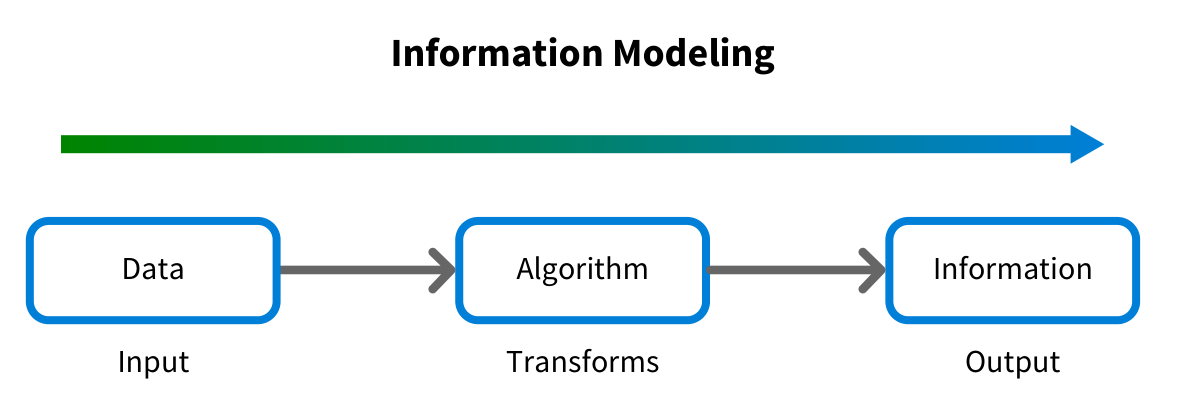
\includegraphics[width=0.95\textwidth,height=0.75\textheight,keepaspectratio]{../textbookForPractice/Figures/Ch_06/ILLUSTRATION 6.1.png}
    \end{figure}
\end{frame}

\begin{frame}{ILLUSTRATION 6.2}

    \begin{figure}[h]
        \centering
        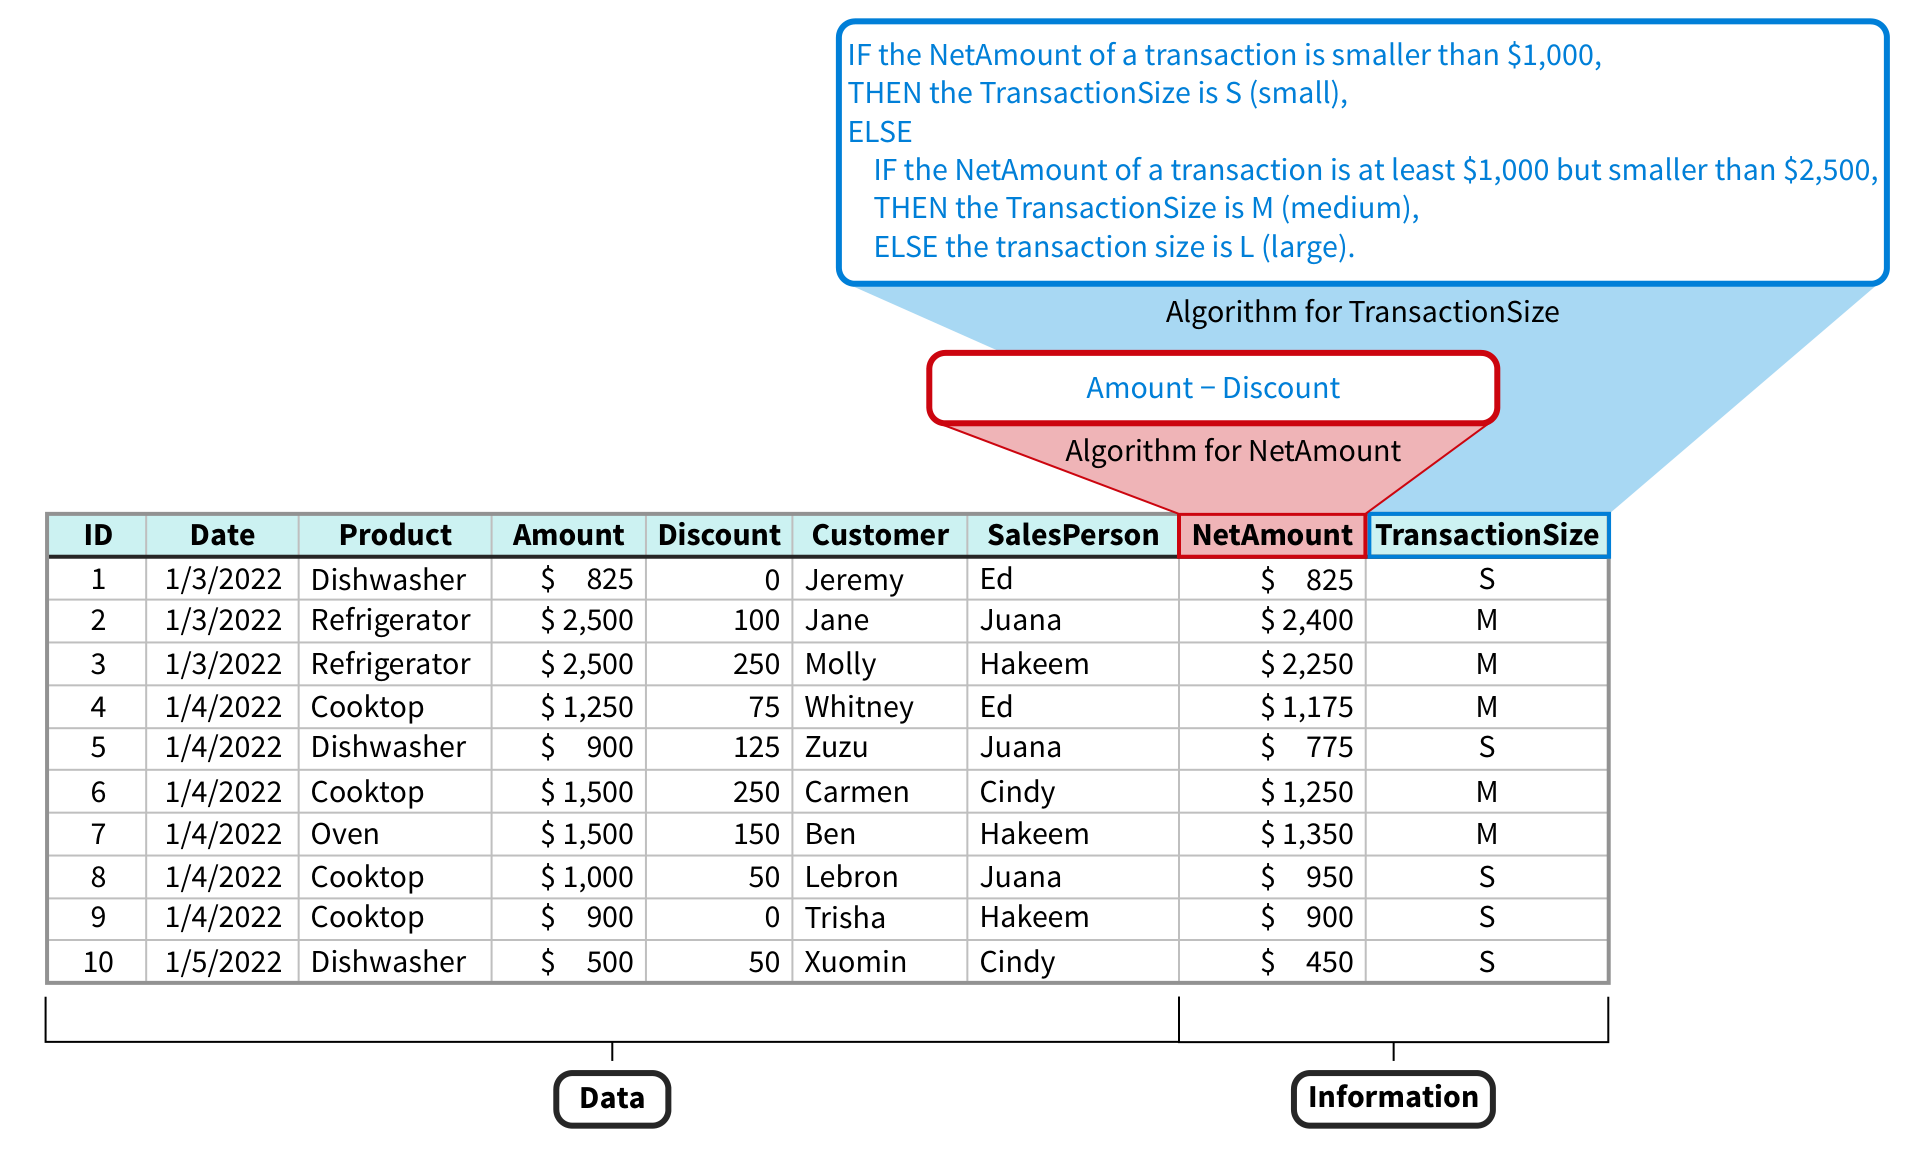
\includegraphics[width=0.95\textwidth,height=0.75\textheight,keepaspectratio]{../textbookForPractice/Figures/Ch_06/ILLUSTRATION 6.2.png}
    \end{figure}
\end{frame}

\begin{frame}{ILLUSTRATION 6.3}

    \begin{figure}[h]
        \centering
        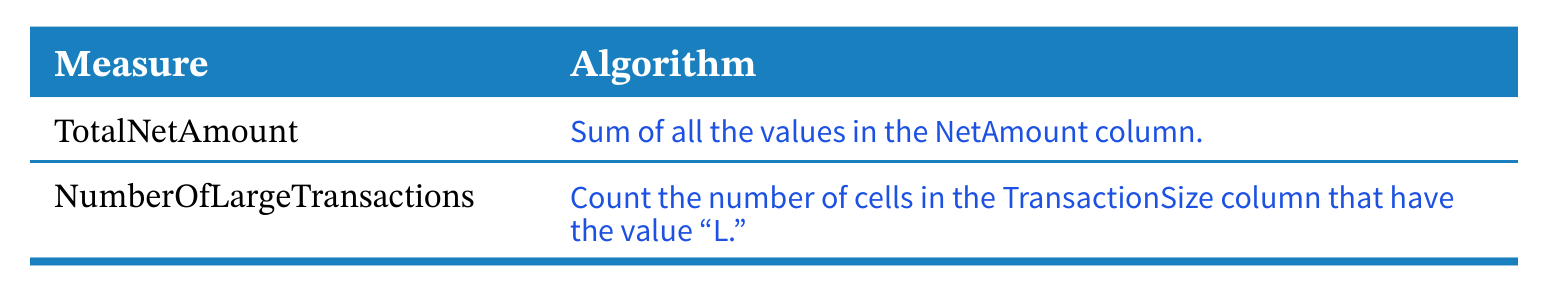
\includegraphics[width=0.95\textwidth,height=0.75\textheight,keepaspectratio]{../textbookForPractice/Figures/Ch_06/ILLUSTRATION 6.3.png}
    \end{figure}
\end{frame}

\begin{frame}{ILLUSTRATION 6.4}

    \begin{figure}[h]
        \centering
        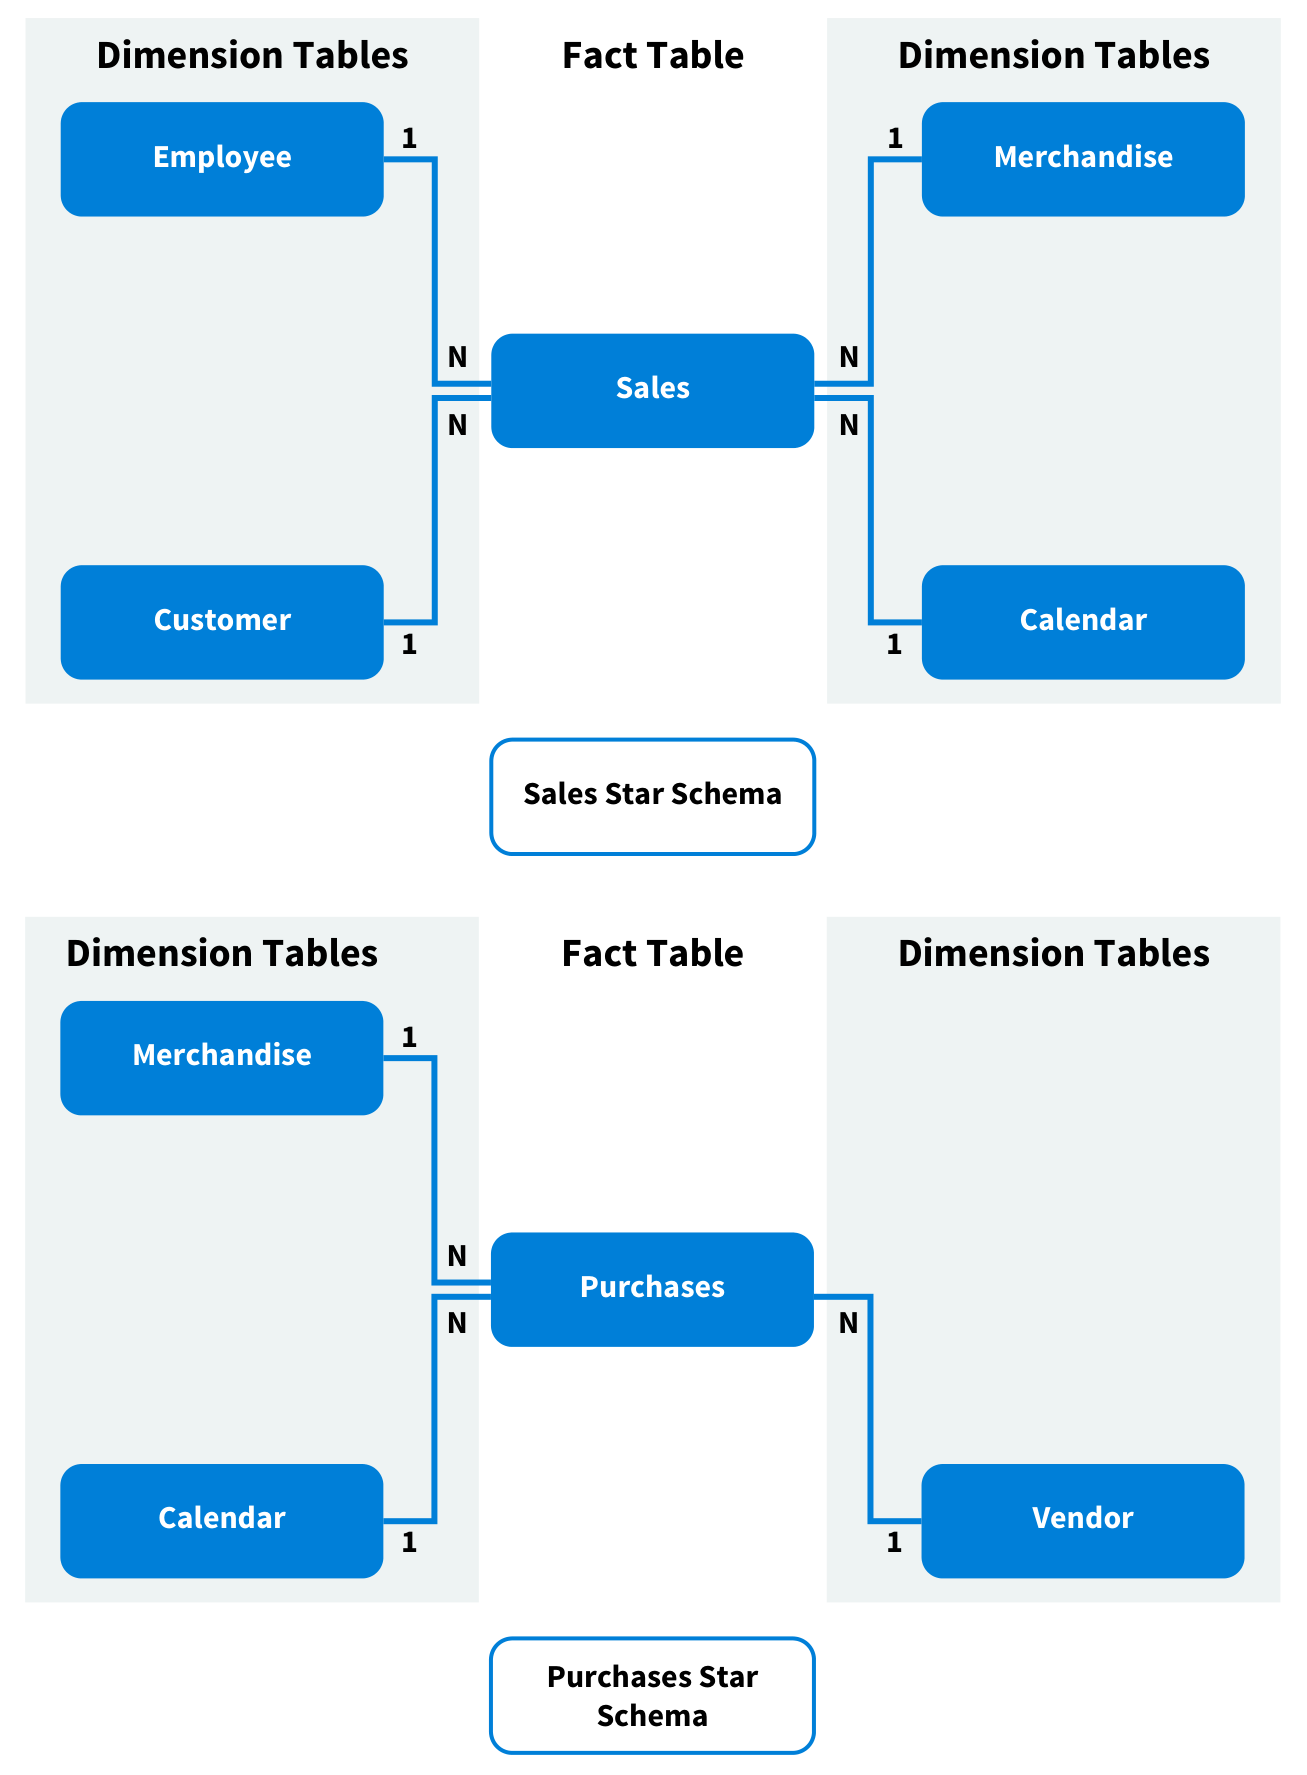
\includegraphics[width=0.95\textwidth,height=0.75\textheight,keepaspectratio]{../textbookForPractice/Figures/Ch_06/ILLUSTRATION 6.4.png}
    \end{figure}
\end{frame}

\begin{frame}{ILLUSTRATION 6.5}

    \begin{figure}[h]
        \centering
        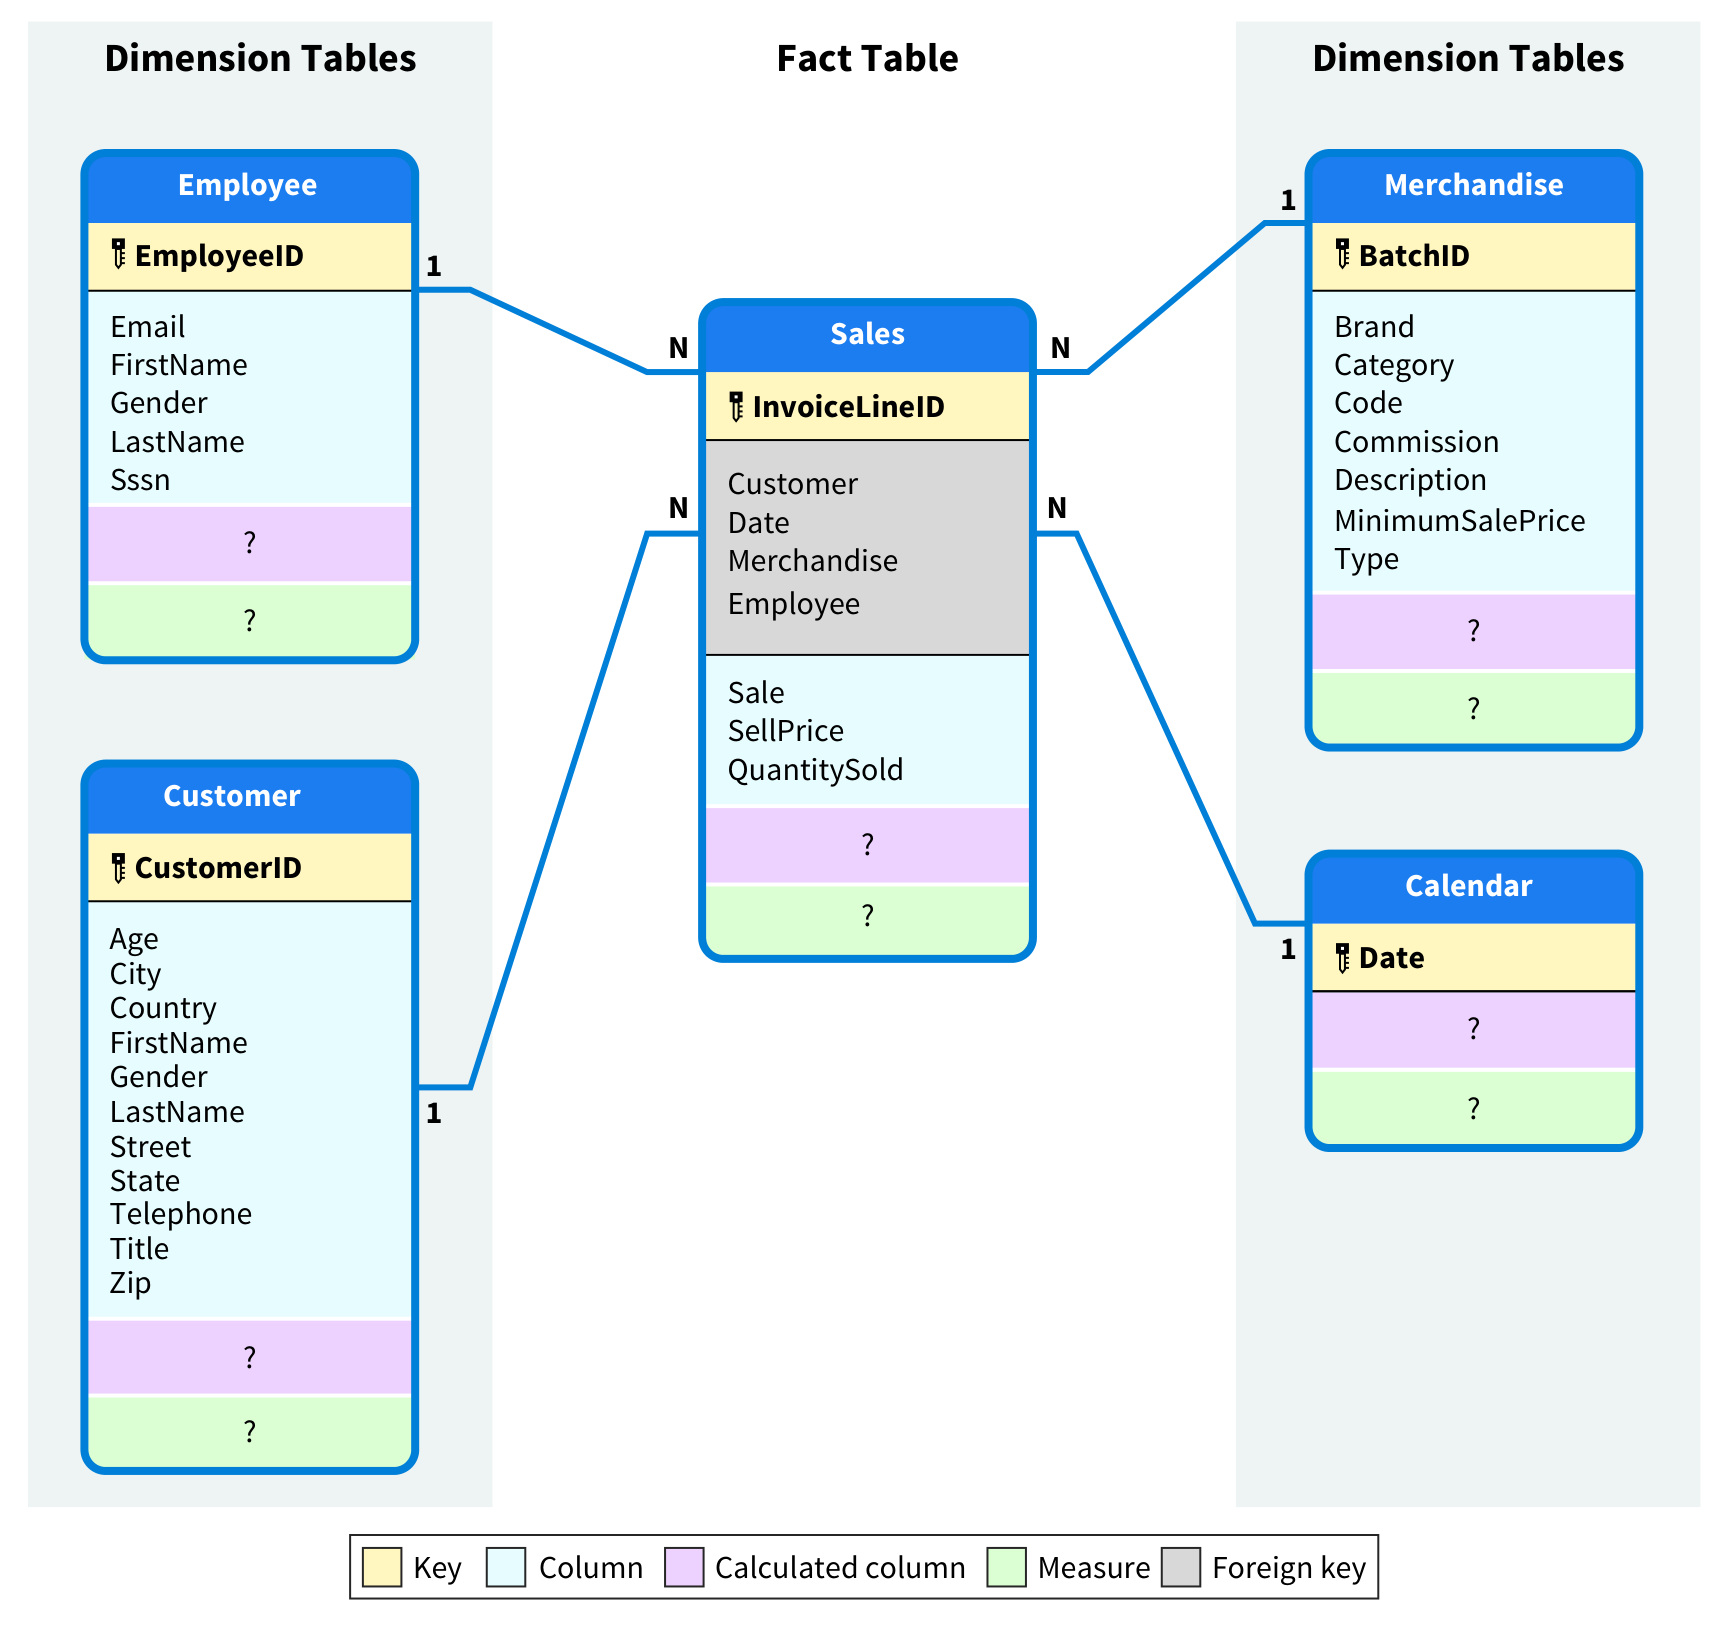
\includegraphics[width=0.95\textwidth,height=0.75\textheight,keepaspectratio]{../textbookForPractice/Figures/Ch_06/ILLUSTRATION 6.5.png}
    \end{figure}
\end{frame}

\begin{frame}{ILLUSTRATION 6.6}

    \begin{figure}[h]
        \centering
        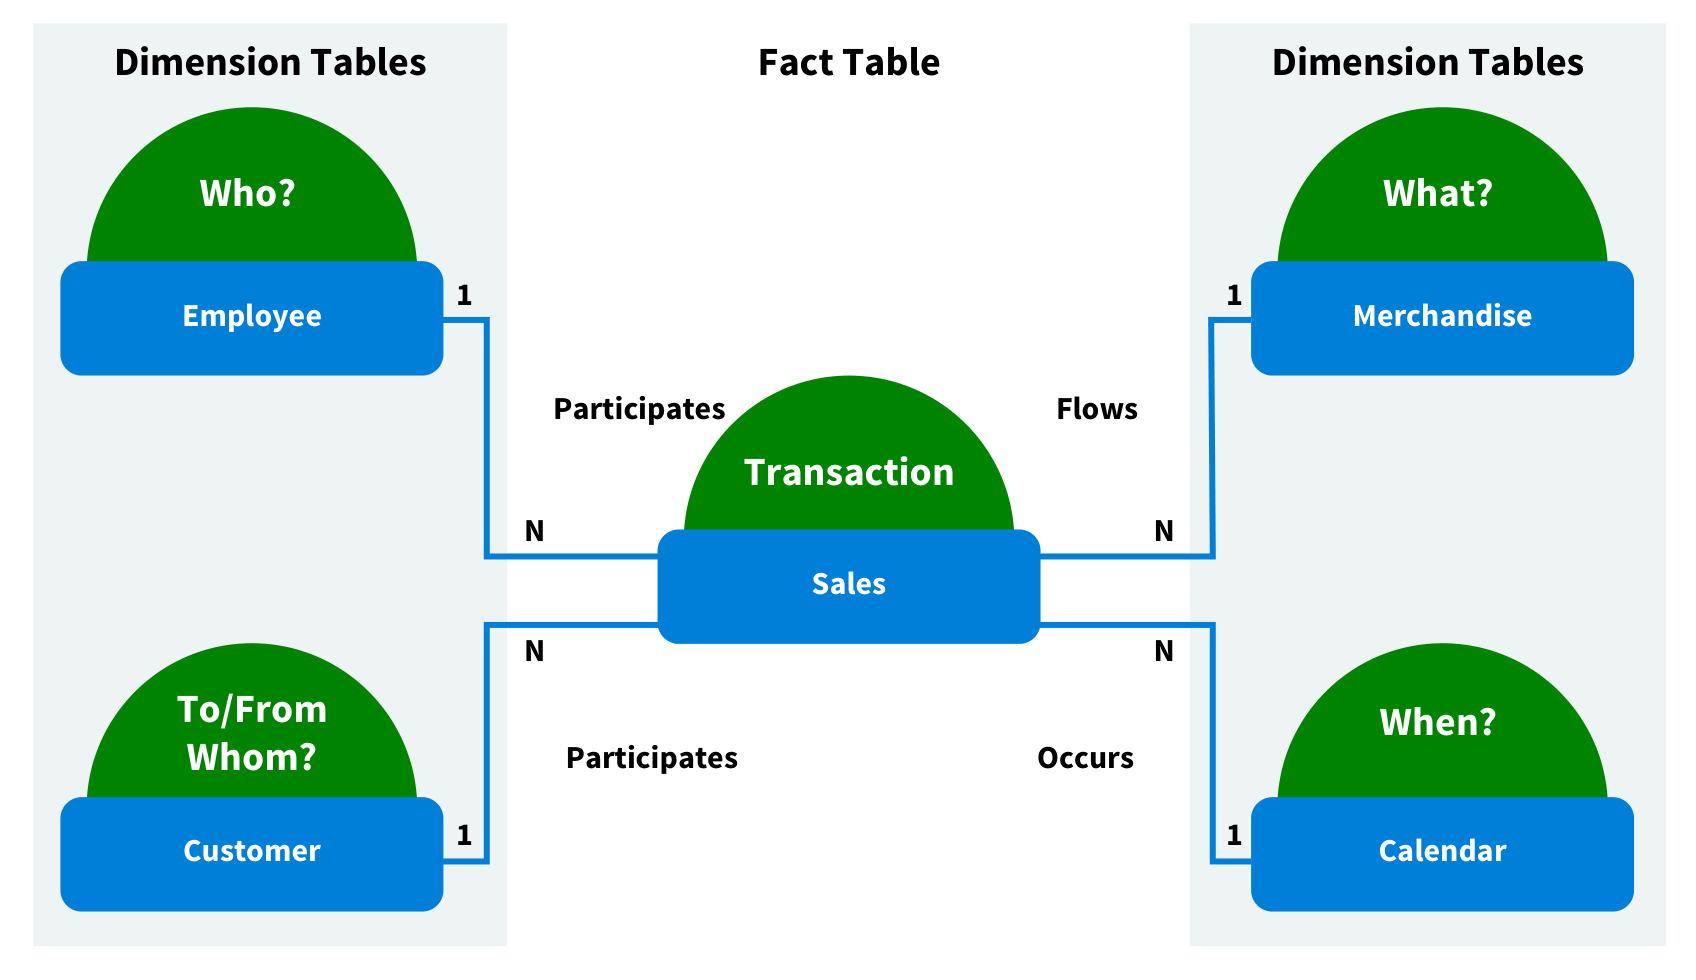
\includegraphics[width=0.95\textwidth,height=0.75\textheight,keepaspectratio]{../textbookForPractice/Figures/Ch_06/ILLUSTRATION 6.6.png}
    \end{figure}
\end{frame}

\begin{frame}{ILLUSTRATION 6.7}

    \begin{figure}[h]
        \centering
        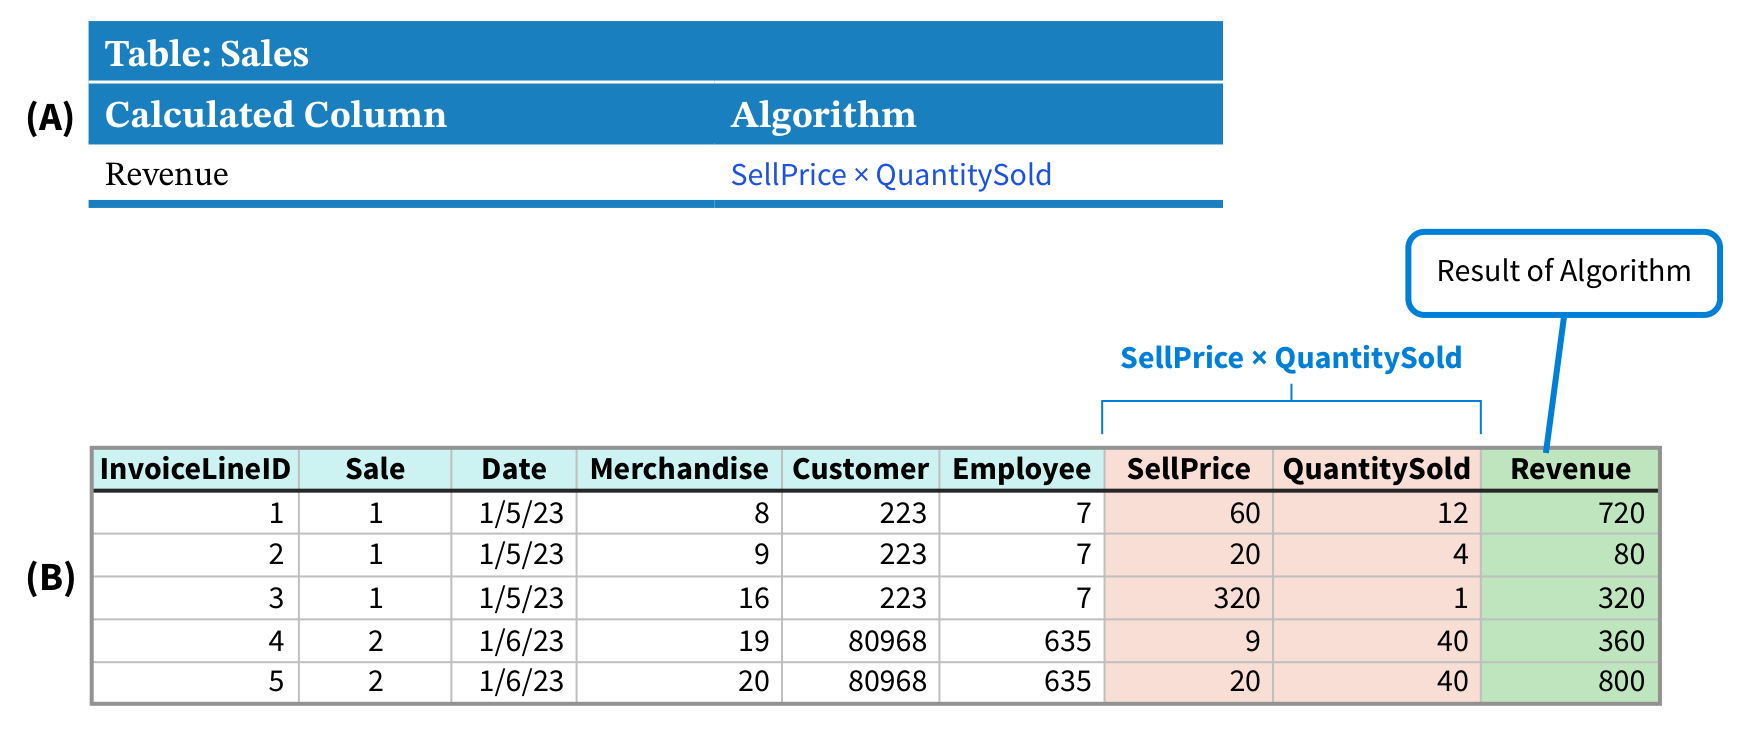
\includegraphics[width=0.95\textwidth,height=0.75\textheight,keepaspectratio]{../textbookForPractice/Figures/Ch_06/ILLUSTRATION 6.7.png}
    \end{figure}
\end{frame}

\begin{frame}{ILLUSTRATION 6.8}

    \begin{figure}[h]
        \centering
        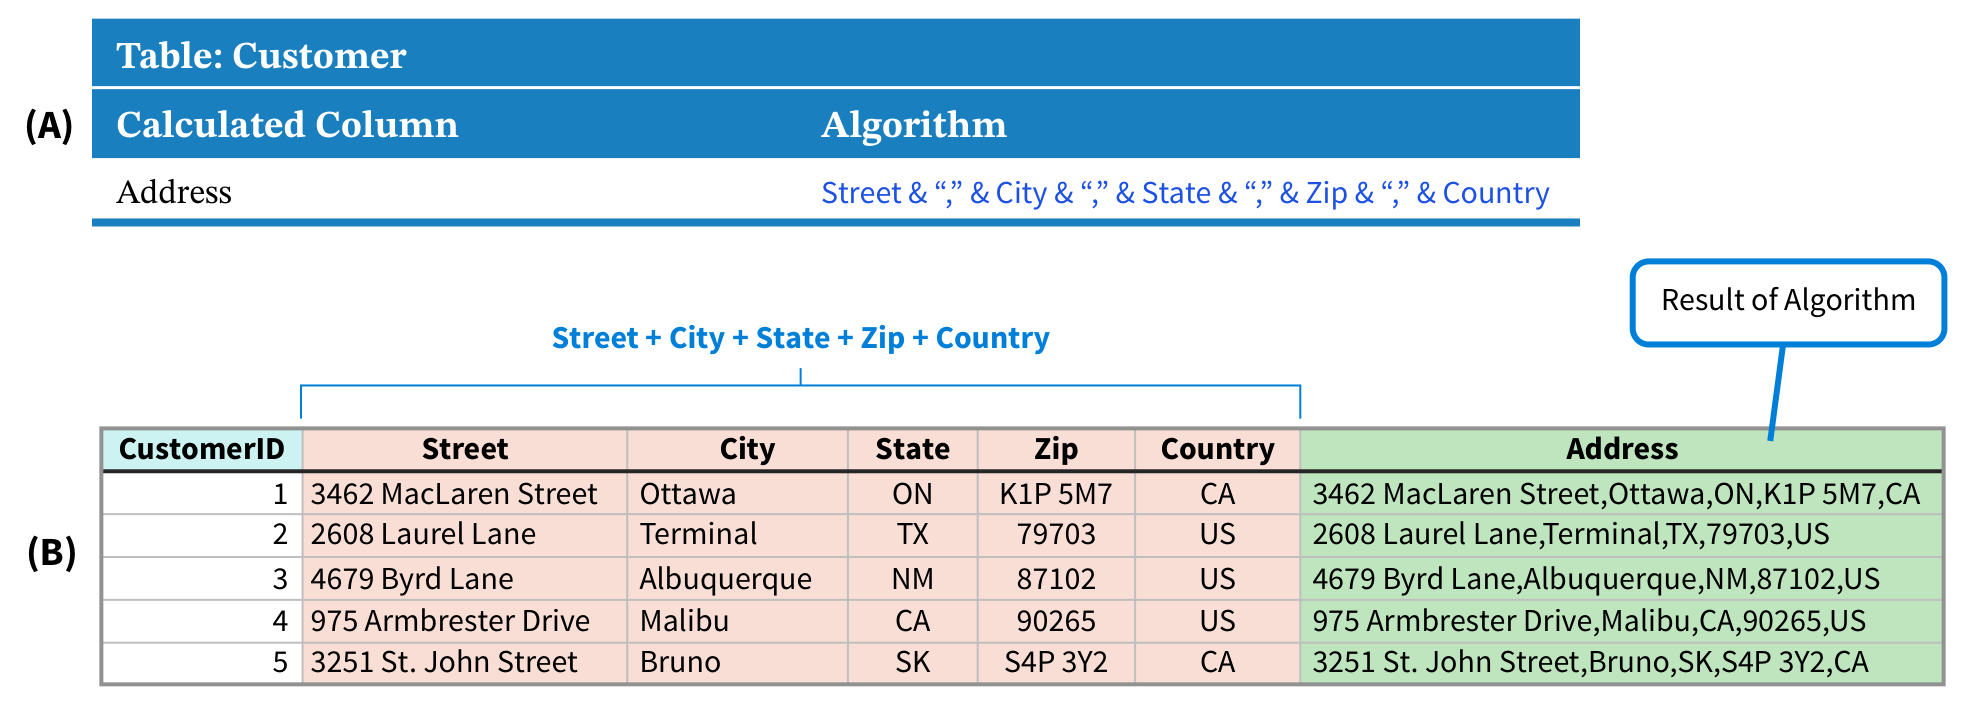
\includegraphics[width=0.95\textwidth,height=0.75\textheight,keepaspectratio]{../textbookForPractice/Figures/Ch_06/ILLUSTRATION 6.8.png}
    \end{figure}
\end{frame}

\begin{frame}{ILLUSTRATION 6.9}

    \begin{figure}[h]
        \centering
        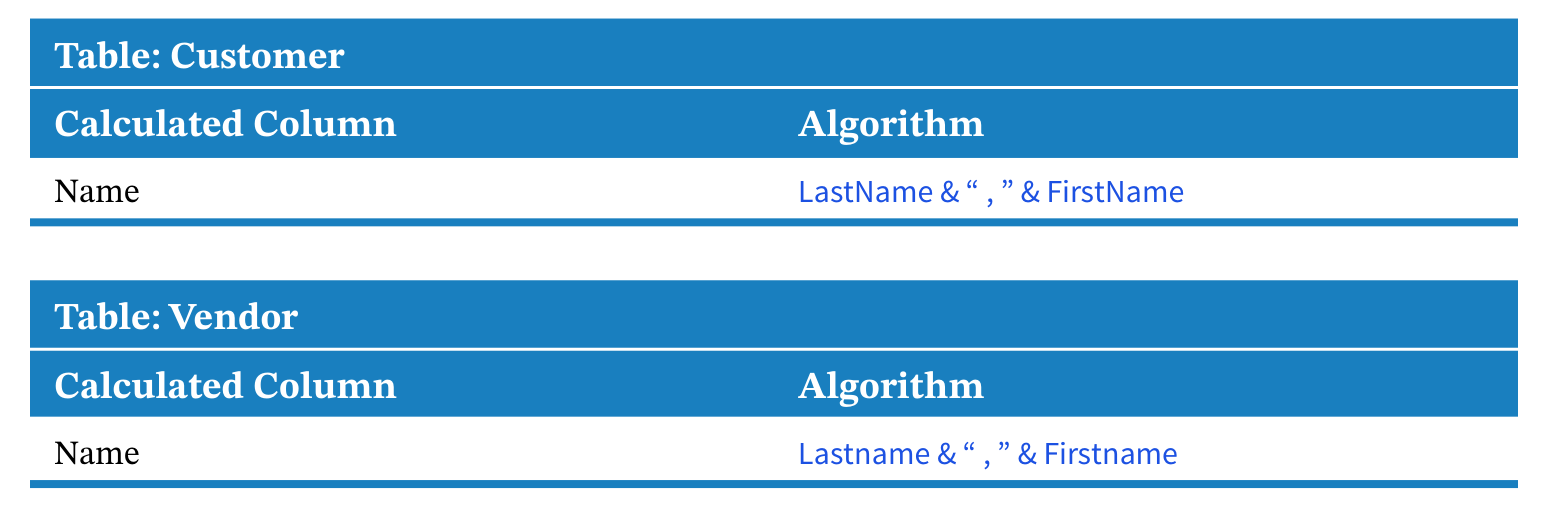
\includegraphics[width=0.95\textwidth,height=0.75\textheight,keepaspectratio]{../textbookForPractice/Figures/Ch_06/ILLUSTRATION 6.9.png}
    \end{figure}
\end{frame}

\begin{frame}{ILLUSTRATION 6.10}

    \begin{figure}[h]
        \centering
        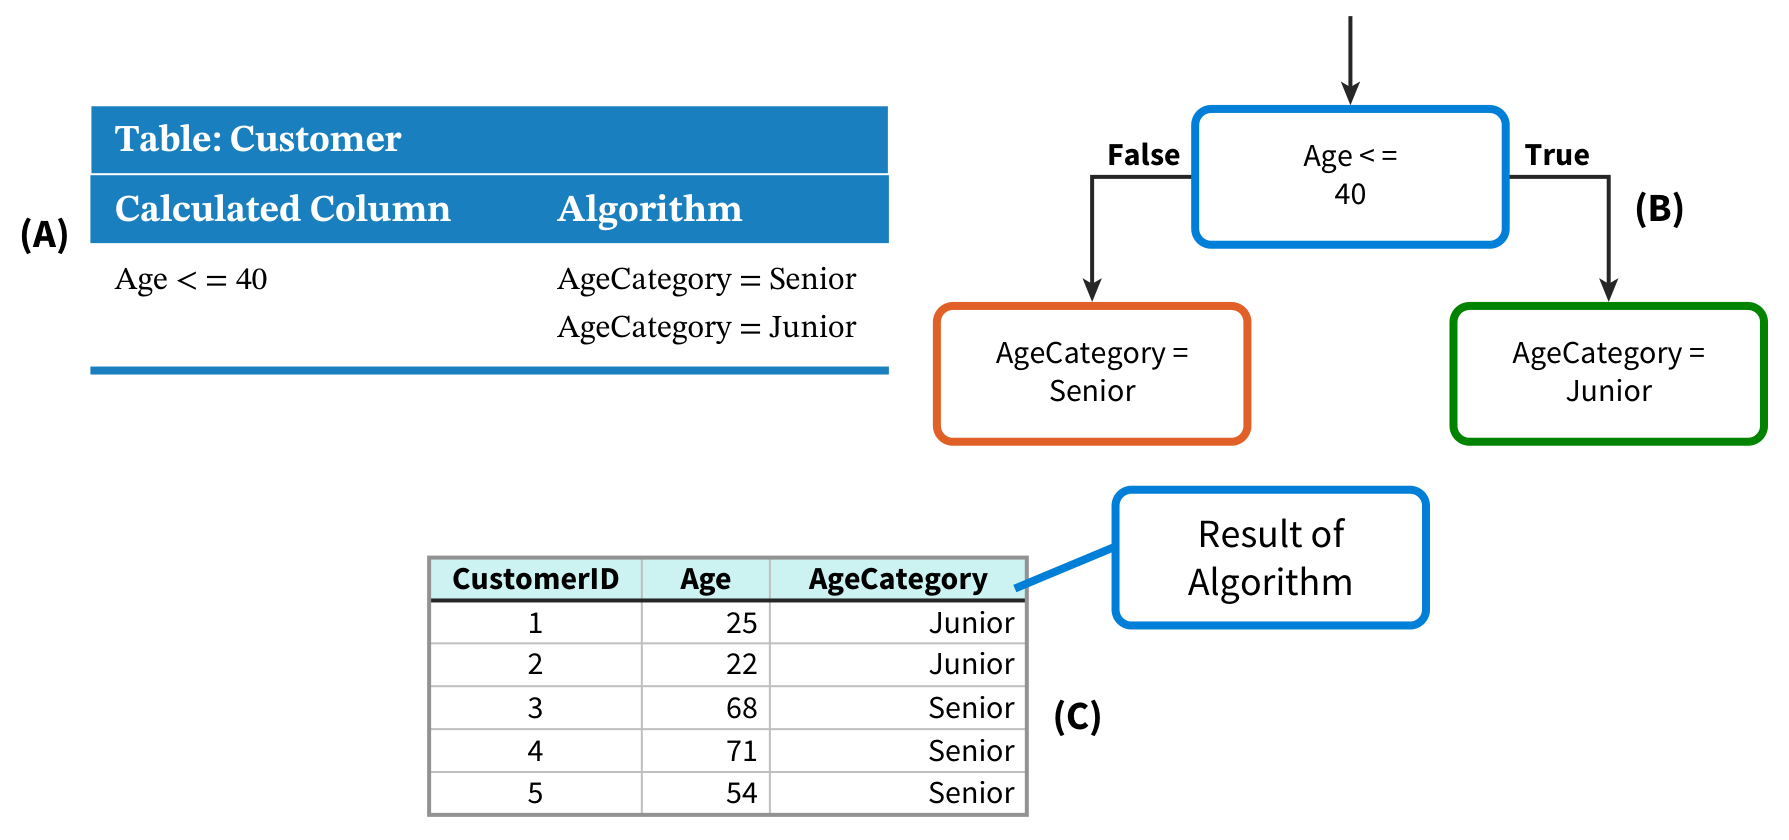
\includegraphics[width=0.95\textwidth,height=0.75\textheight,keepaspectratio]{../textbookForPractice/Figures/Ch_06/ILLUSTRATION 6.10.png}
    \end{figure}
\end{frame}

\begin{frame}{ILLUSTRATION 6.11}

    \begin{figure}[h]
        \centering
        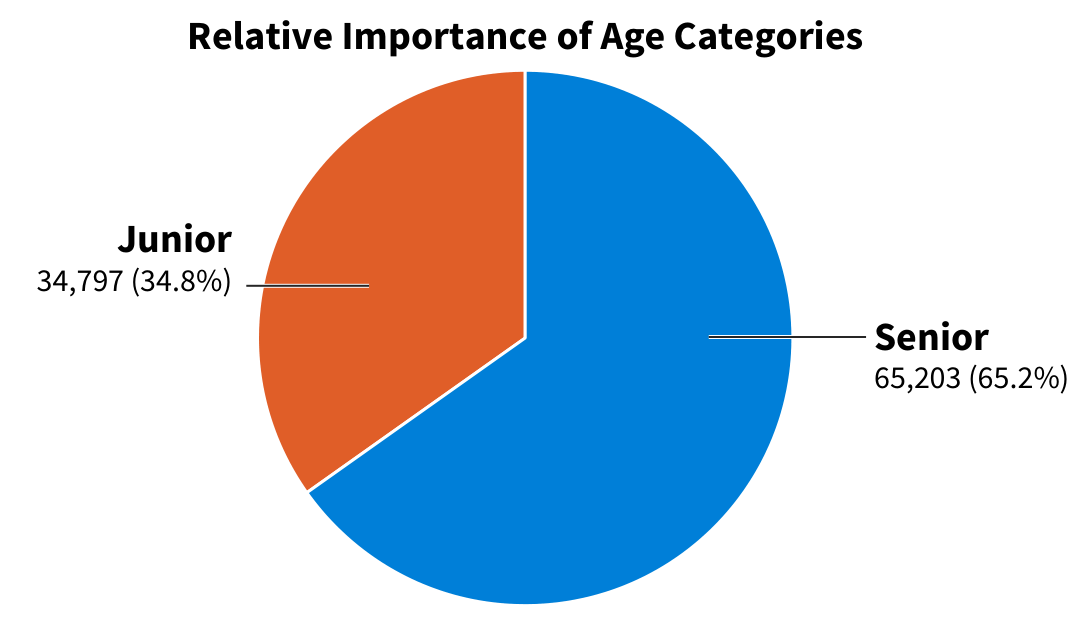
\includegraphics[width=0.95\textwidth,height=0.75\textheight,keepaspectratio]{../textbookForPractice/Figures/Ch_06/ILLUSTRATION 6.11.png}
    \end{figure}
\end{frame}

\begin{frame}{Thuật toán và Phương pháp tiếp cận}
\begin{itemize}
    \item \textbf{Thuật toán (Algorithms):} Là tập hợp các quy tắc tính toán (ví dụ: Tính biên lợi nhuận = Doanh thu - Giá vốn).
    \item \textbf{Phương pháp tiếp cận có cấu trúc (Structured Approach):} 
    \begin{itemize}
        \item Hiểu rõ yêu cầu đầu ra (Output).
        \item Xác định dữ liệu đầu vào (Input).
        \item Xây dựng các bước xử lý logic (Processing).
    \end{itemize}
\end{itemize}
\end{frame}

\begin{frame}{ILLUSTRATION 6.12}

    \begin{figure}[h]
        \centering
        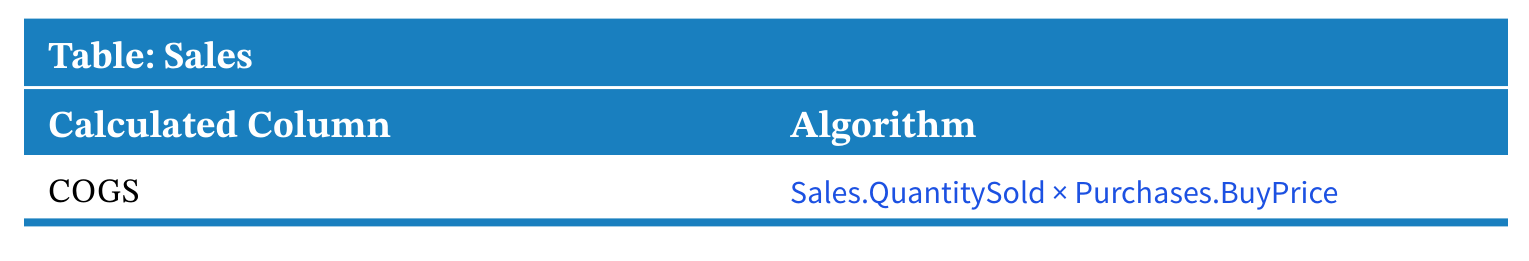
\includegraphics[width=0.95\textwidth,height=0.75\textheight,keepaspectratio]{../textbookForPractice/Figures/Ch_06/ILLUSTRATION 6.12.png}
    \end{figure}
\end{frame}

\begin{frame}{ILLUSTRATION 6.13}

    \begin{figure}[h]
        \centering
        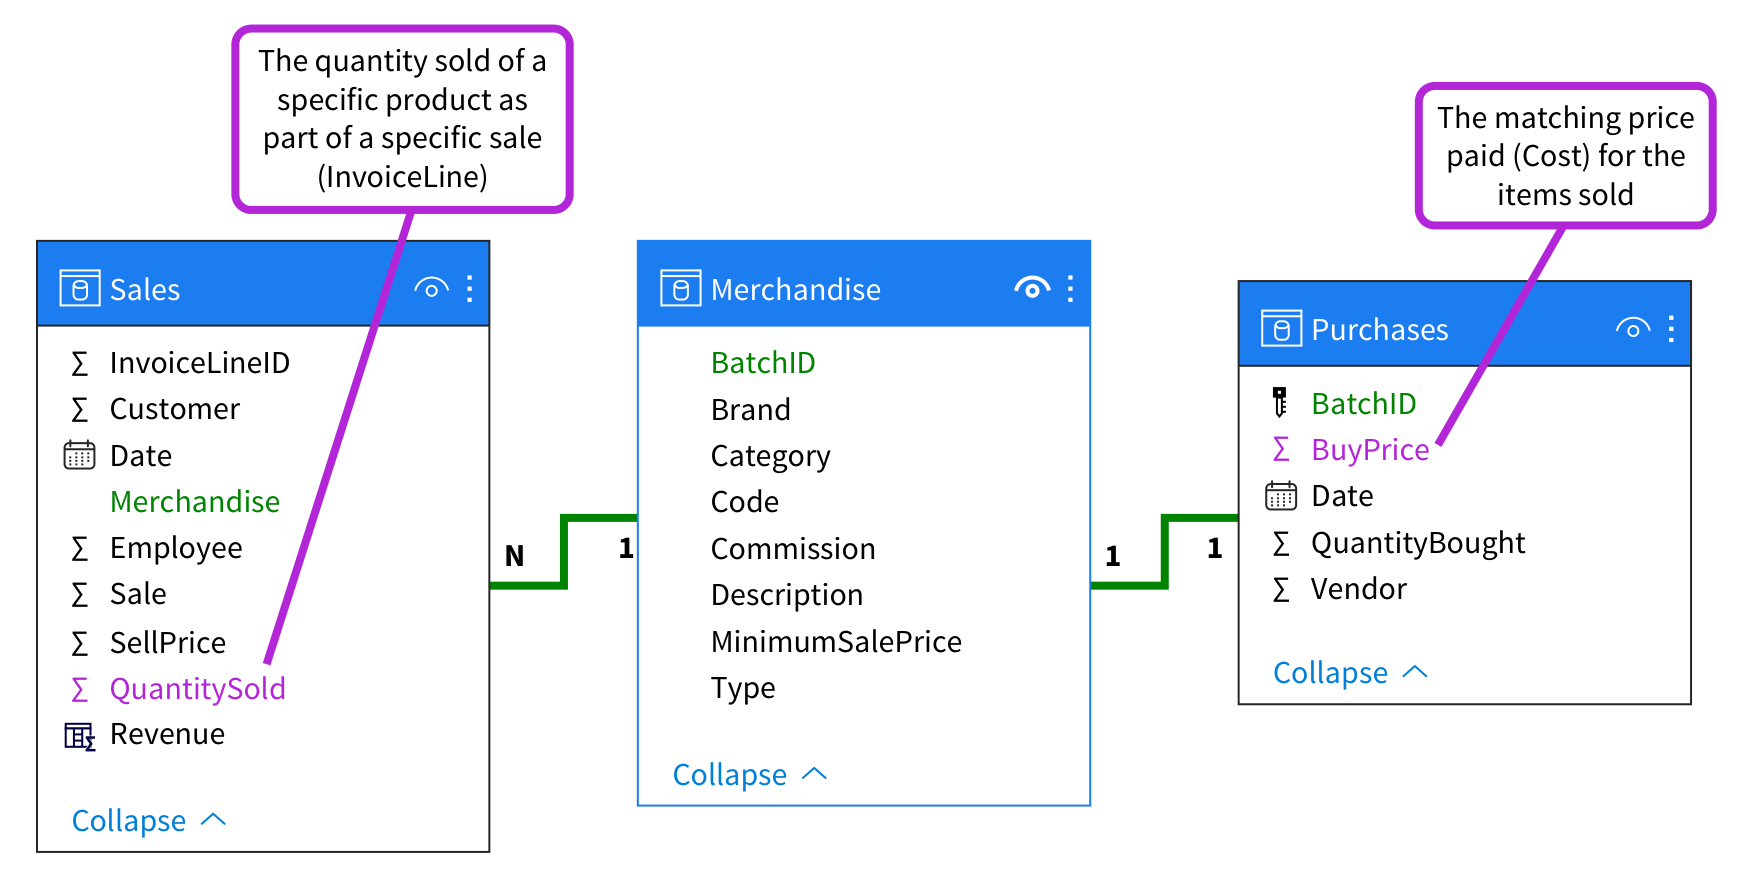
\includegraphics[width=0.95\textwidth,height=0.75\textheight,keepaspectratio]{../textbookForPractice/Figures/Ch_06/ILLUSTRATION 6.13.png}
    \end{figure}
\end{frame}

\begin{frame}{ILLUSTRATION 6.14}

    \begin{figure}[h]
        \centering
        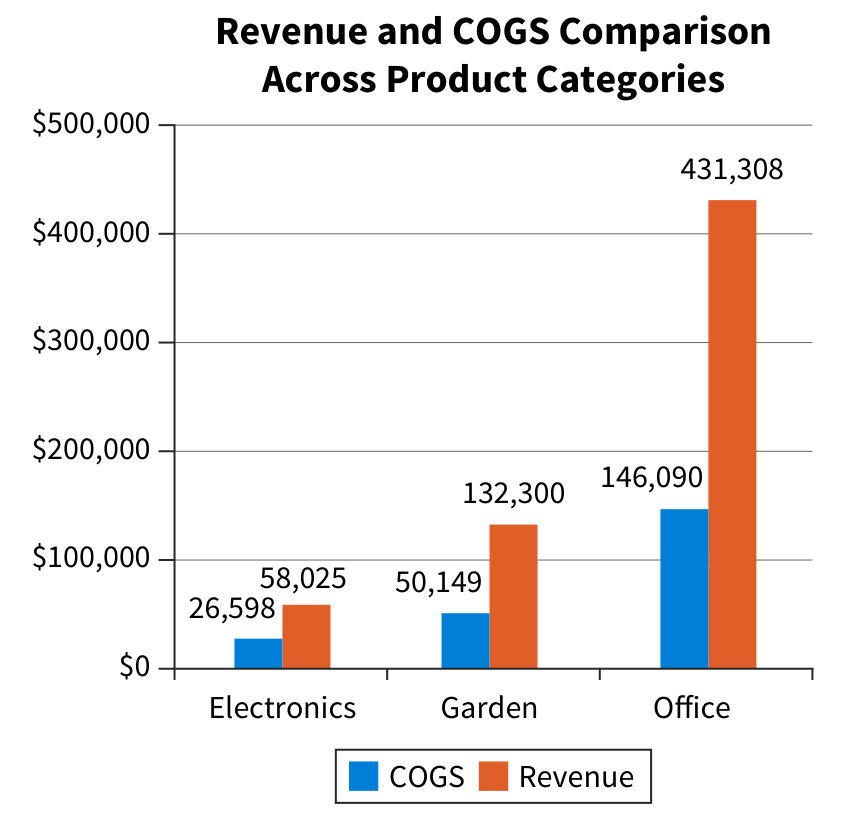
\includegraphics[width=0.95\textwidth,height=0.75\textheight,keepaspectratio]{../textbookForPractice/Figures/Ch_06/ILLUSTRATION 6.14.png}
    \end{figure}
\end{frame}

\begin{frame}{ILLUSTRATION 6.15}

    \begin{figure}[h]
        \centering
        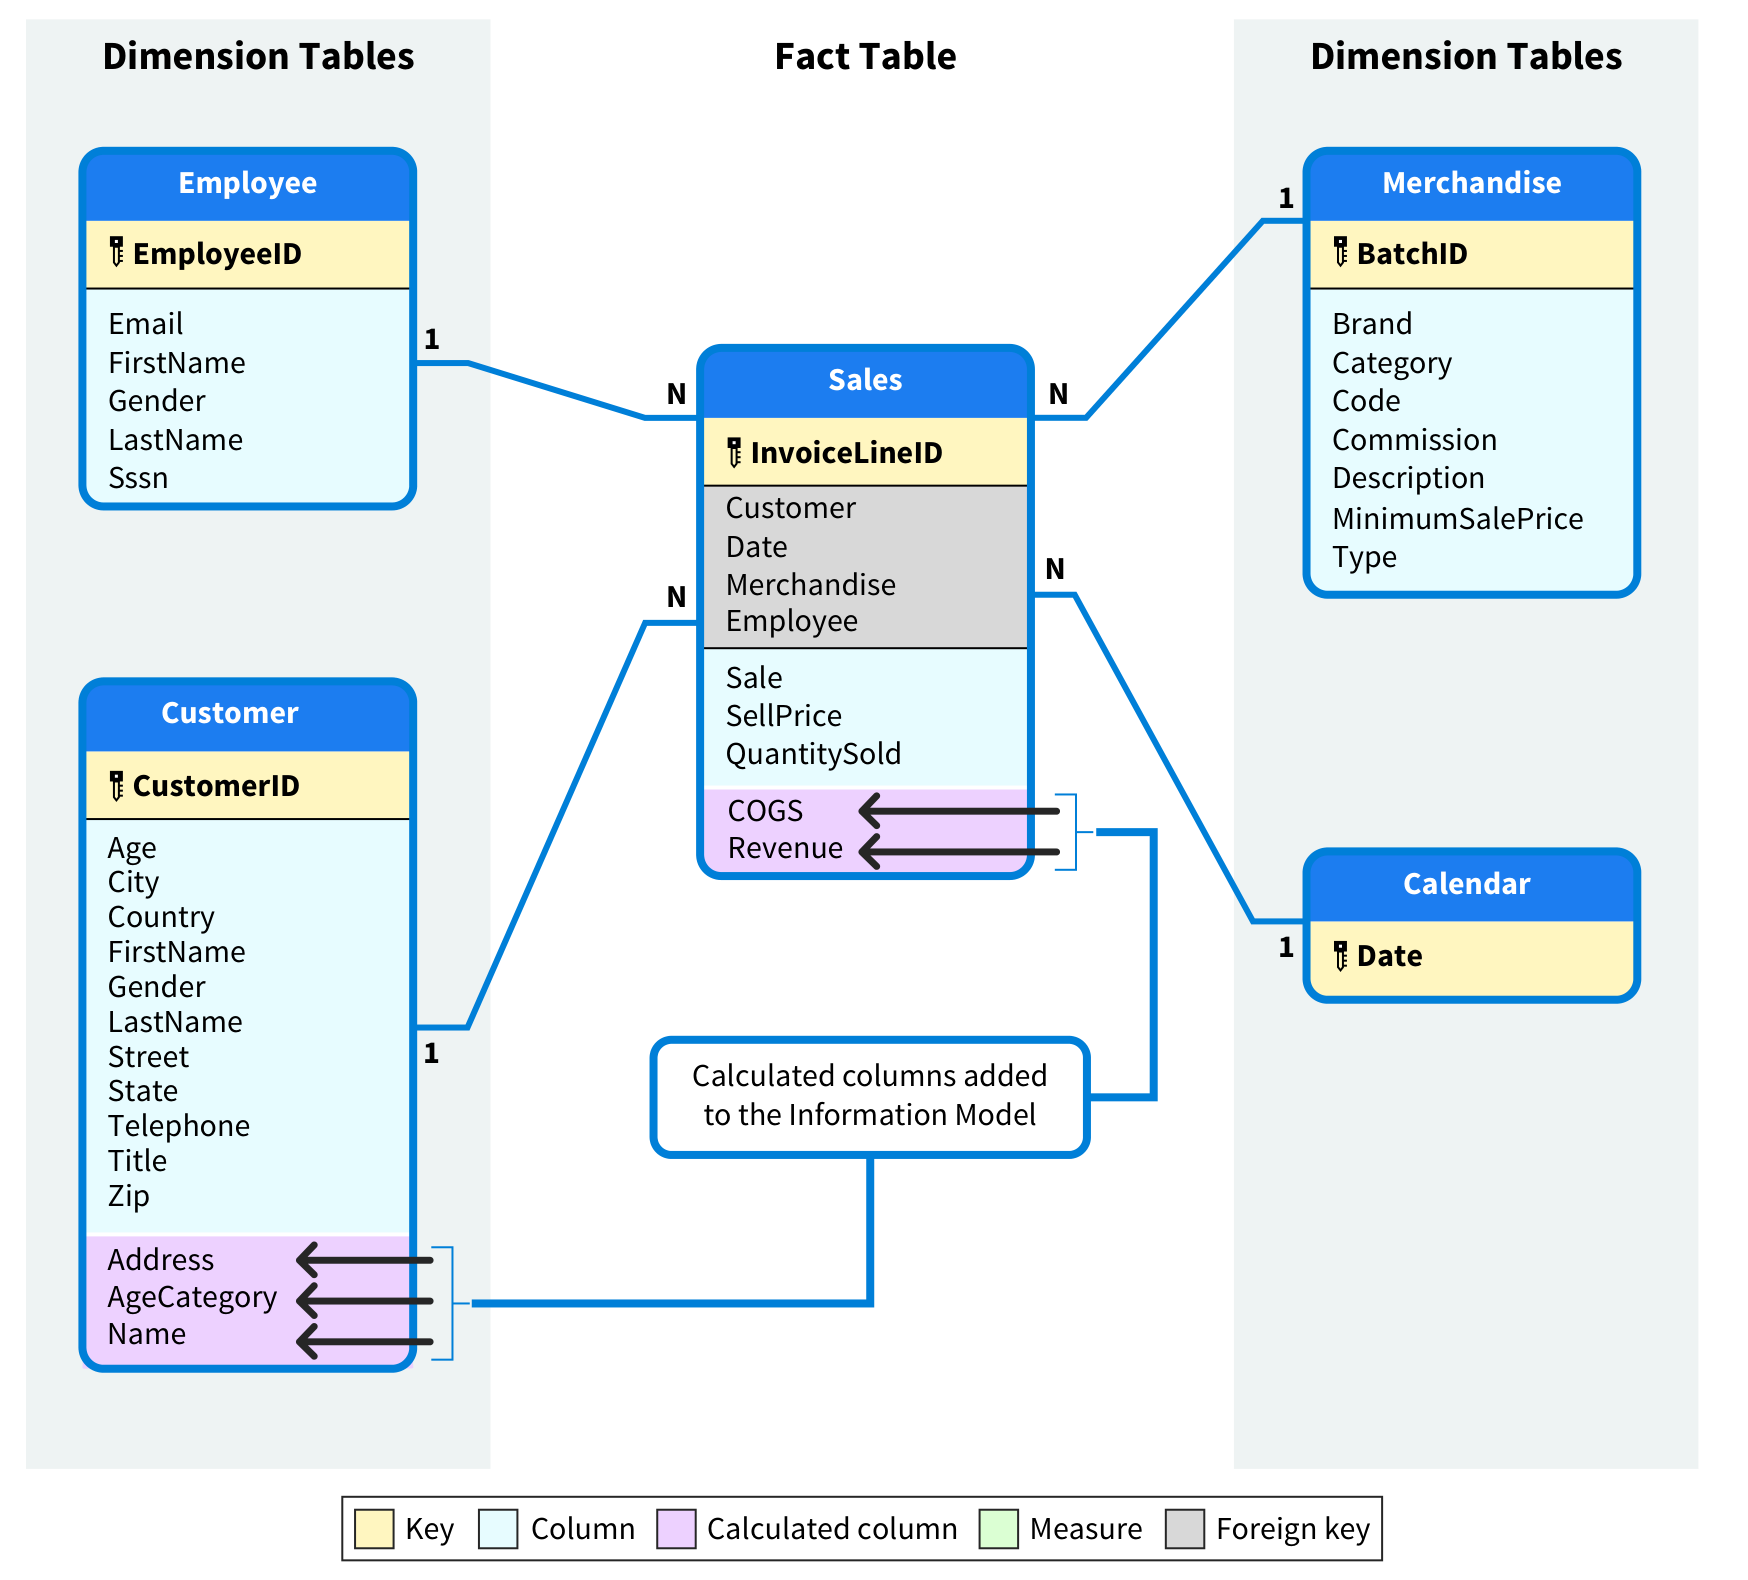
\includegraphics[width=0.95\textwidth,height=0.75\textheight,keepaspectratio]{../textbookForPractice/Figures/Ch_06/ILLUSTRATION 6.15.png}
    \end{figure}
\end{frame}

\begin{frame}{ILLUSTRATION 6.16}

    \begin{figure}[h]
        \centering
        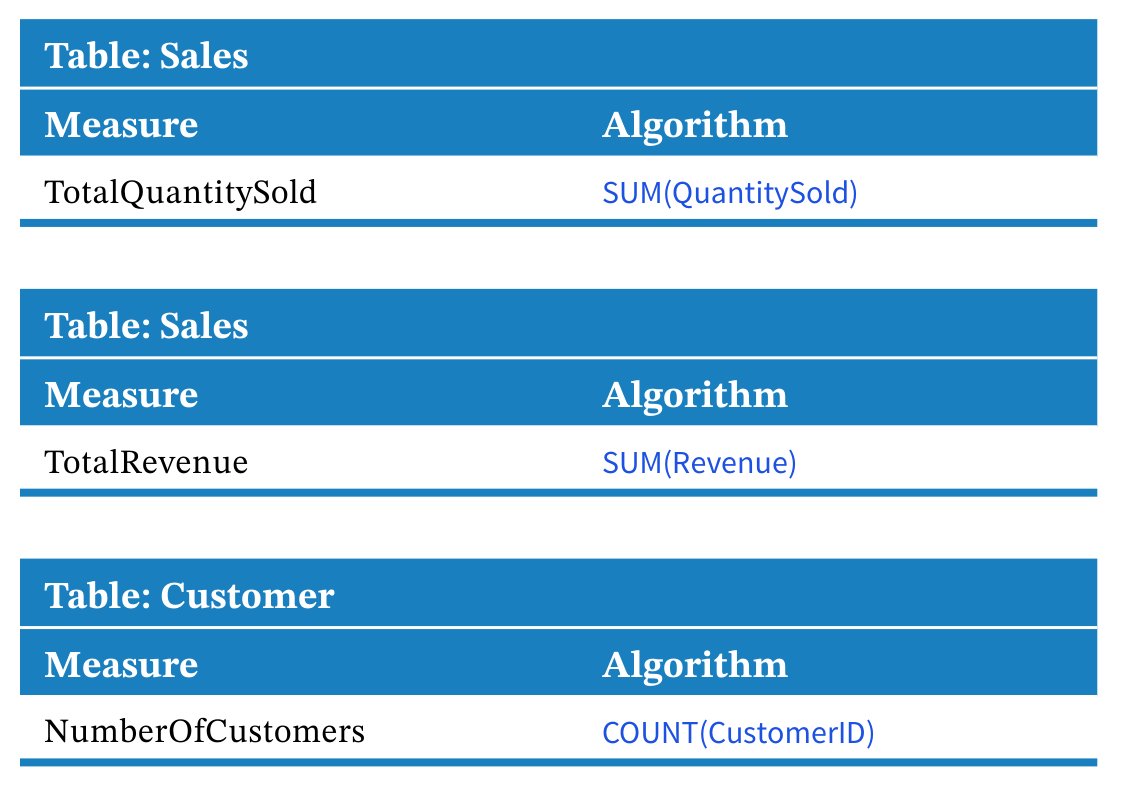
\includegraphics[width=0.95\textwidth,height=0.75\textheight,keepaspectratio]{../textbookForPractice/Figures/Ch_06/ILLUSTRATION 6.16.png}
    \end{figure}
\end{frame}

\begin{frame}{ILLUSTRATION 6.17}

    \begin{figure}[h]
        \centering
        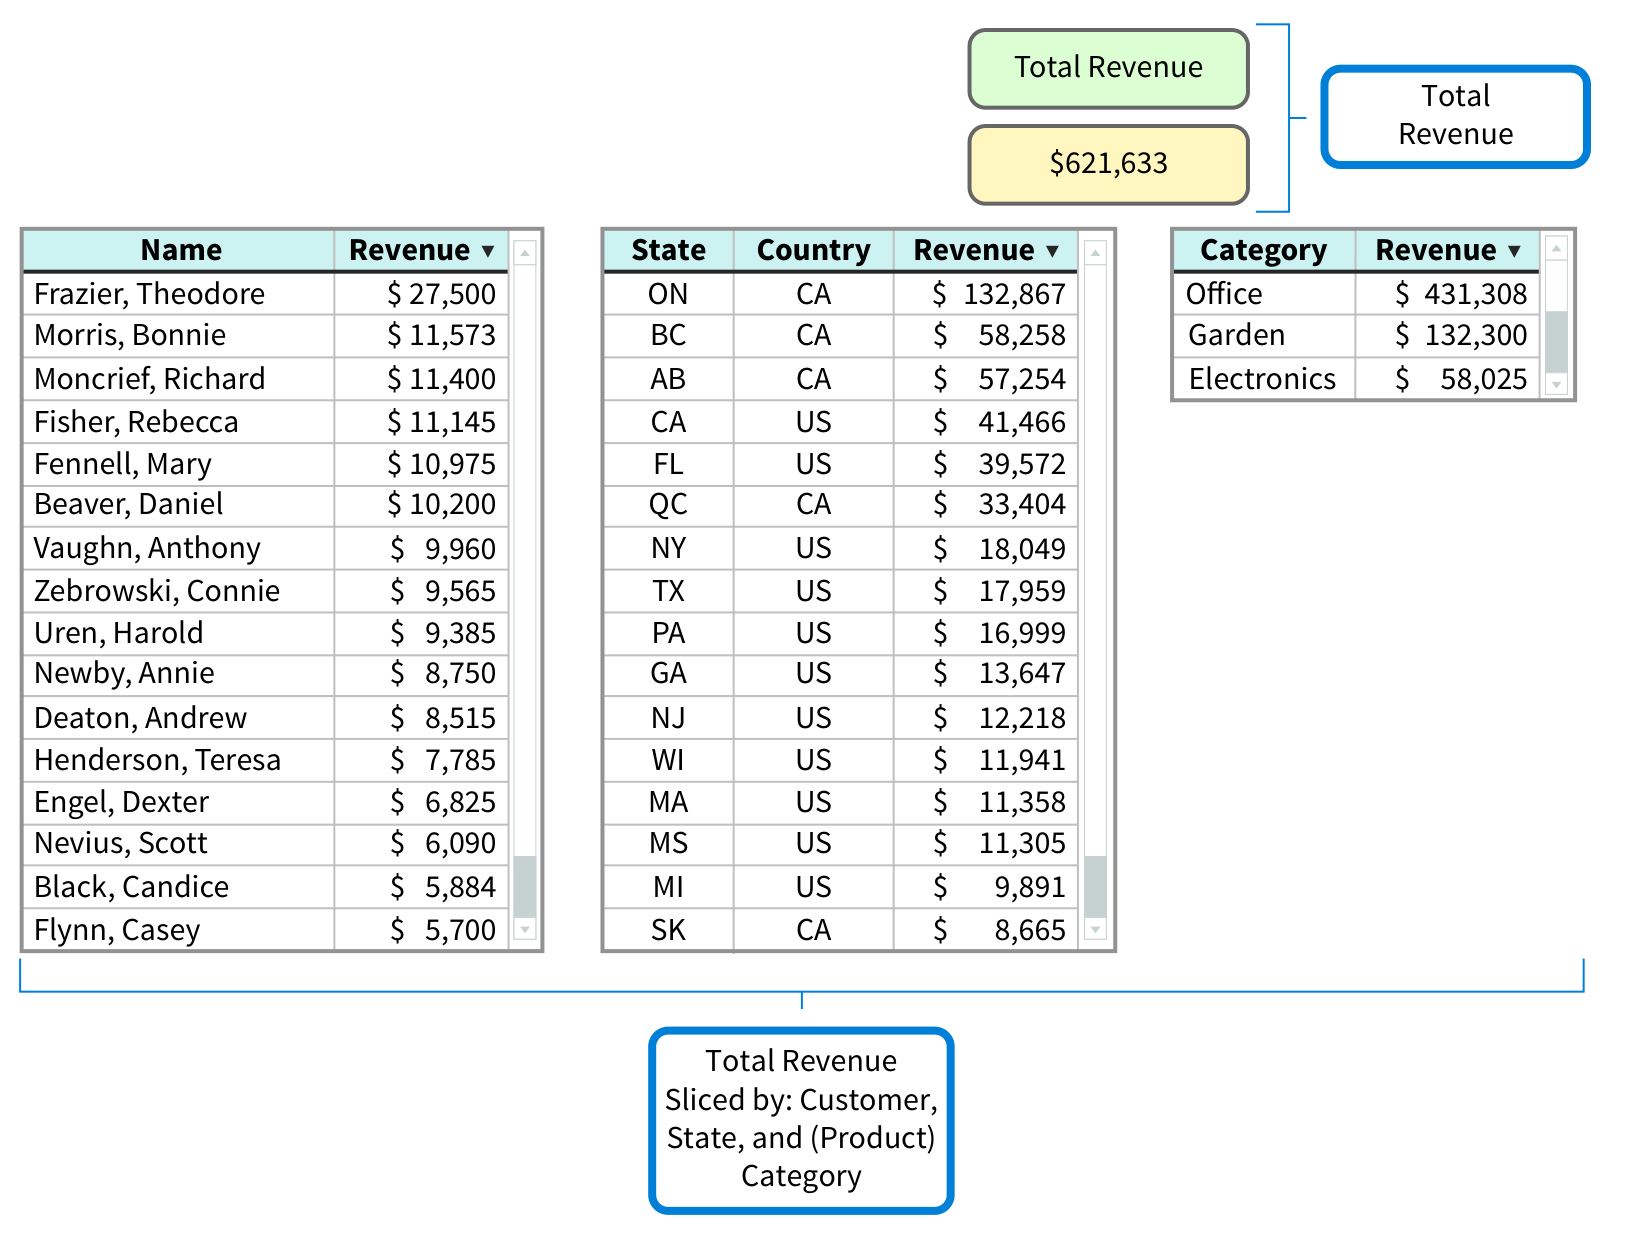
\includegraphics[width=0.95\textwidth,height=0.75\textheight,keepaspectratio]{../textbookForPractice/Figures/Ch_06/ILLUSTRATION 6.17.png}
    \end{figure}
\end{frame}

\begin{frame}{ILLUSTRATION 6.18}

    \begin{figure}[h]
        \centering
        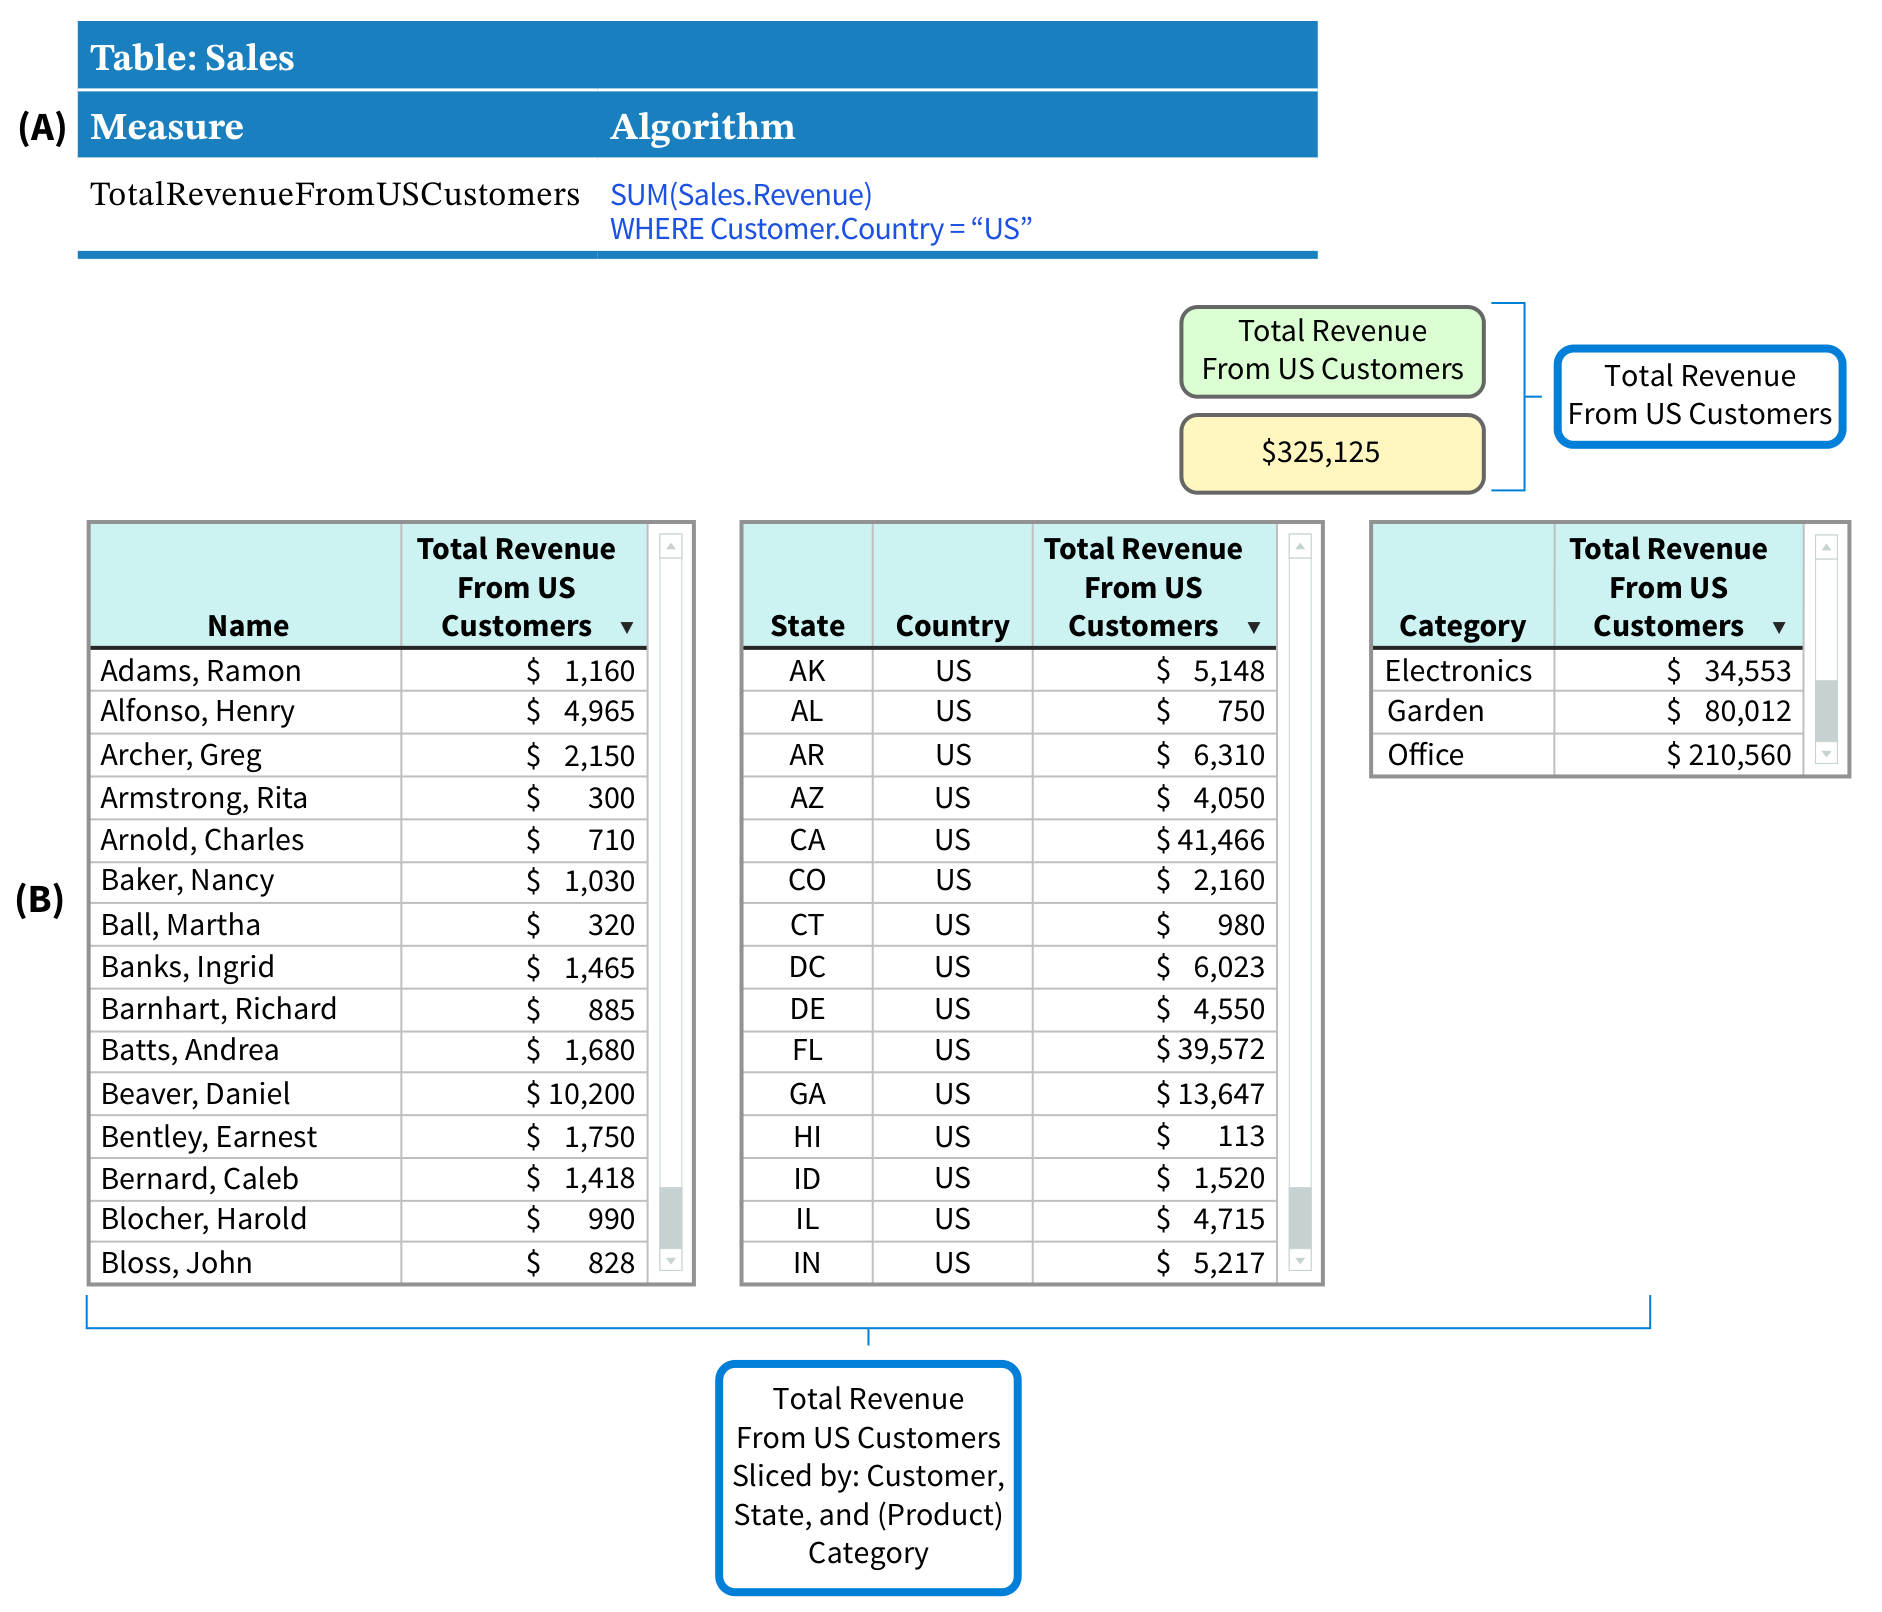
\includegraphics[width=0.95\textwidth,height=0.75\textheight,keepaspectratio]{../textbookForPractice/Figures/Ch_06/ILLUSTRATION 6.18.png}
    \end{figure}
\end{frame}

\begin{frame}{ILLUSTRATION 6.19}

    \begin{figure}[h]
        \centering
        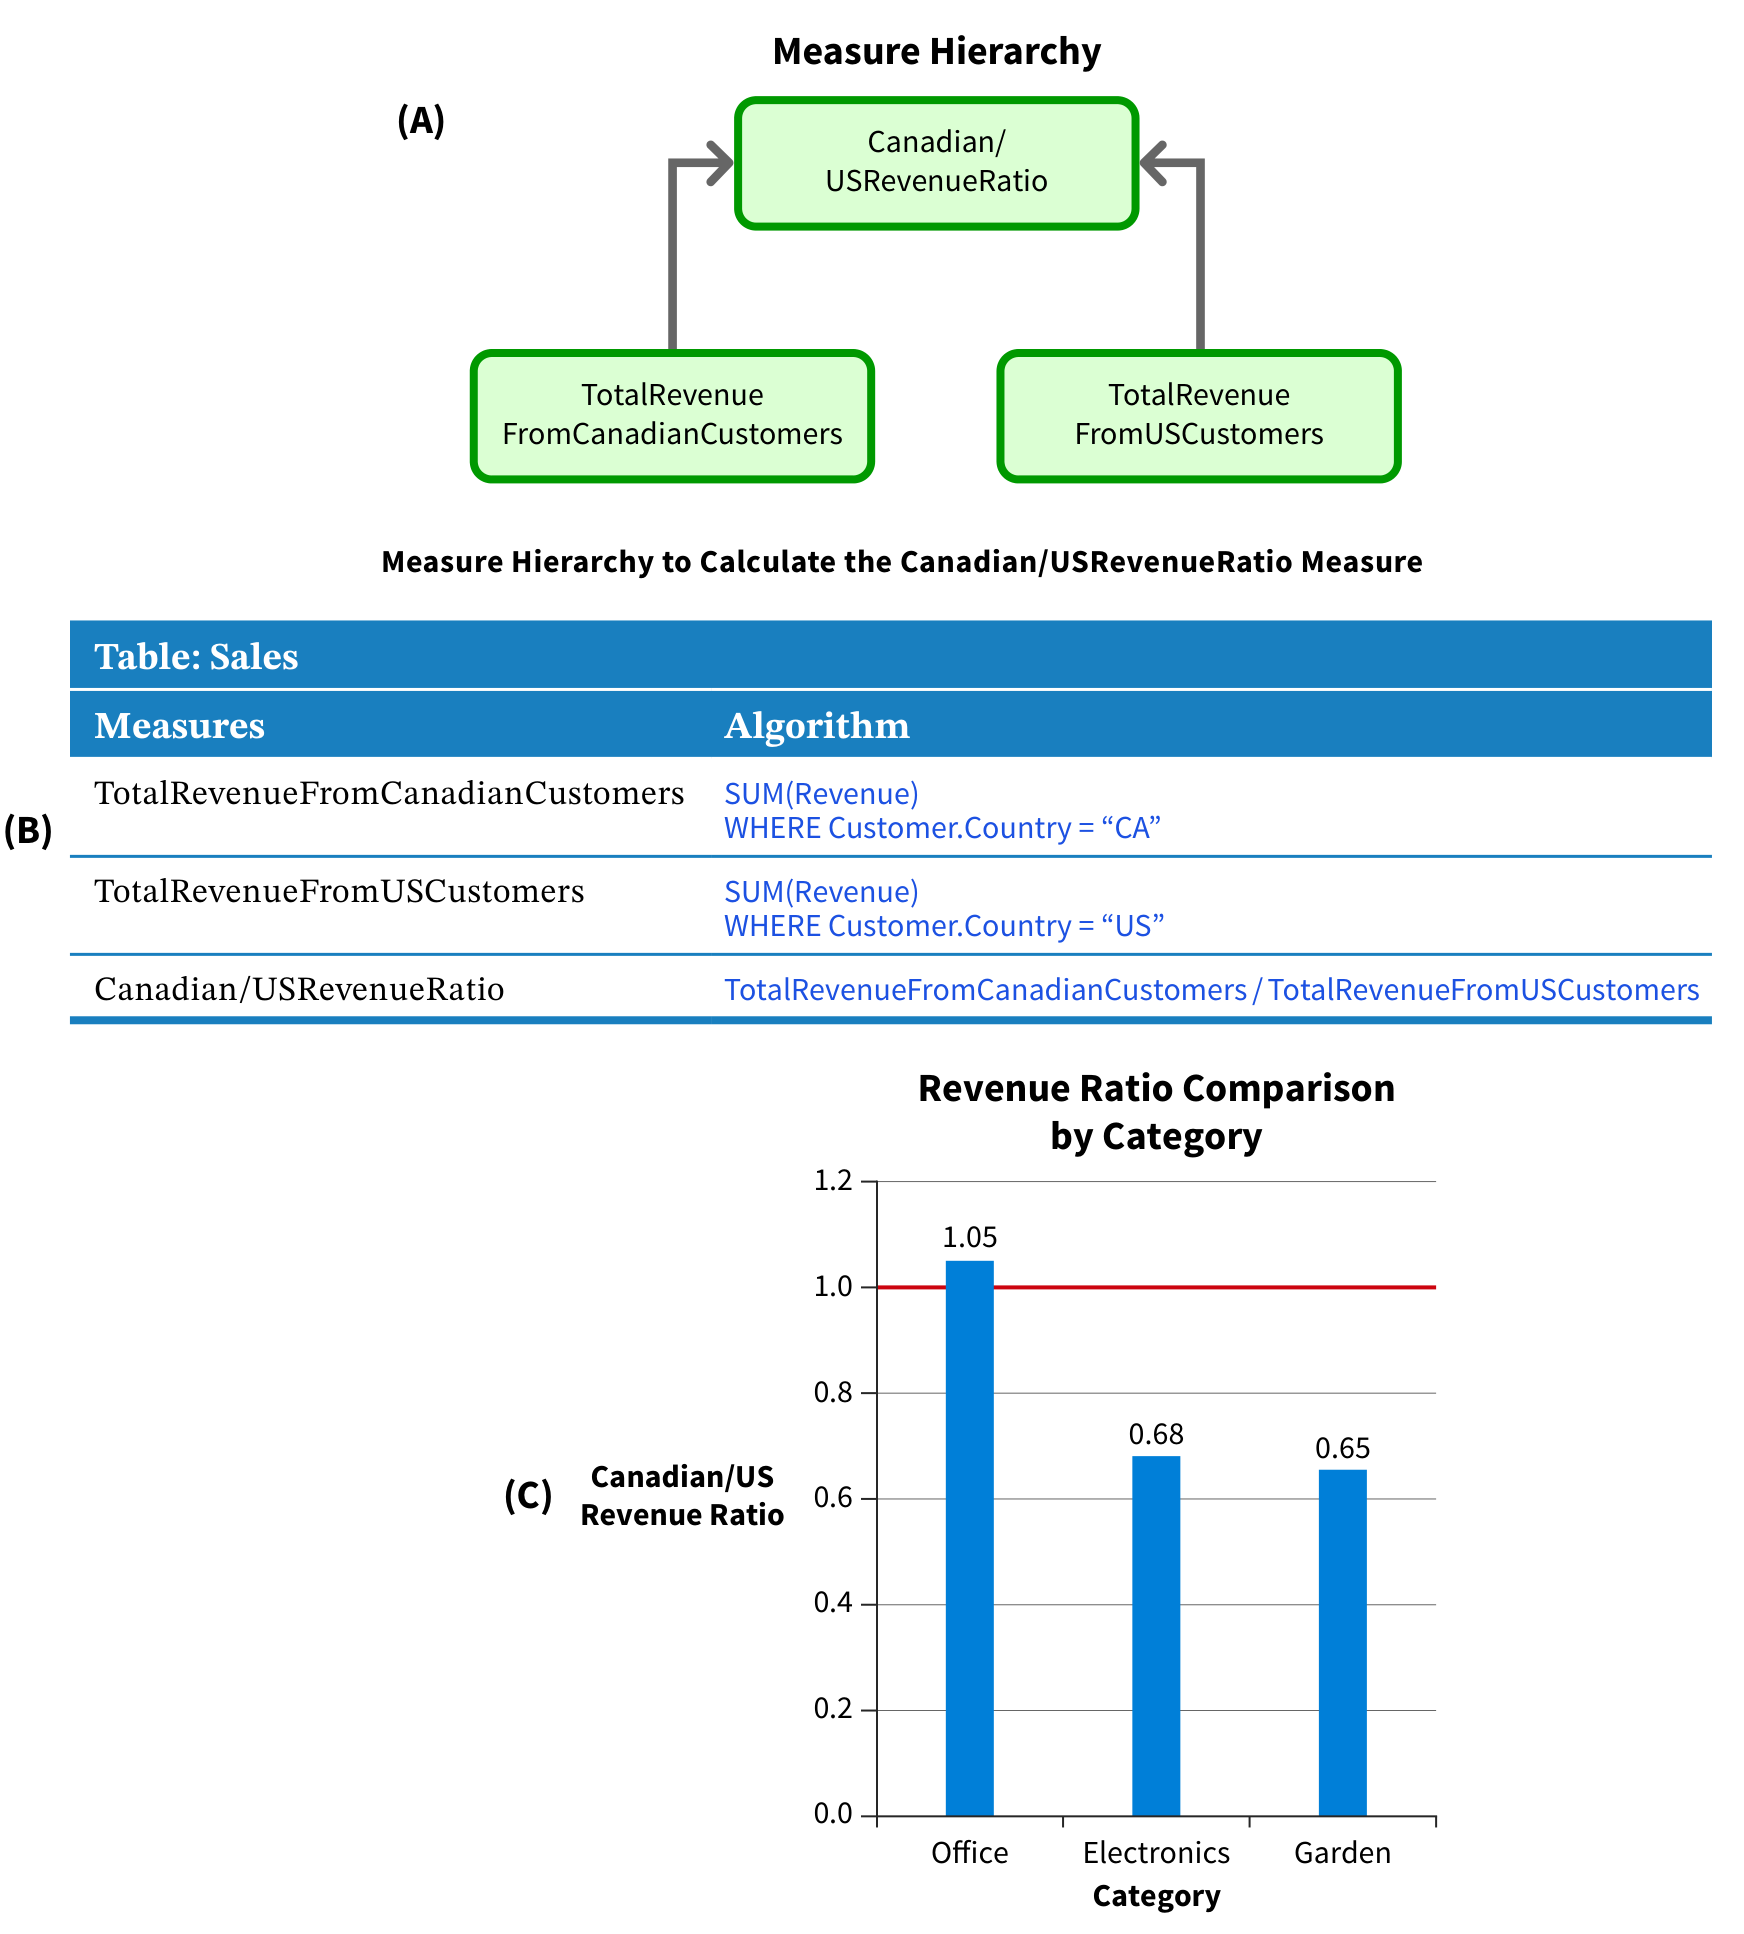
\includegraphics[width=0.95\textwidth,height=0.75\textheight,keepaspectratio]{../textbookForPractice/Figures/Ch_06/ILLUSTRATION 6.19.png}
    \end{figure}
\end{frame}

\begin{frame}{ILLUSTRATION 6.20}

    \begin{figure}[h]
        \centering
        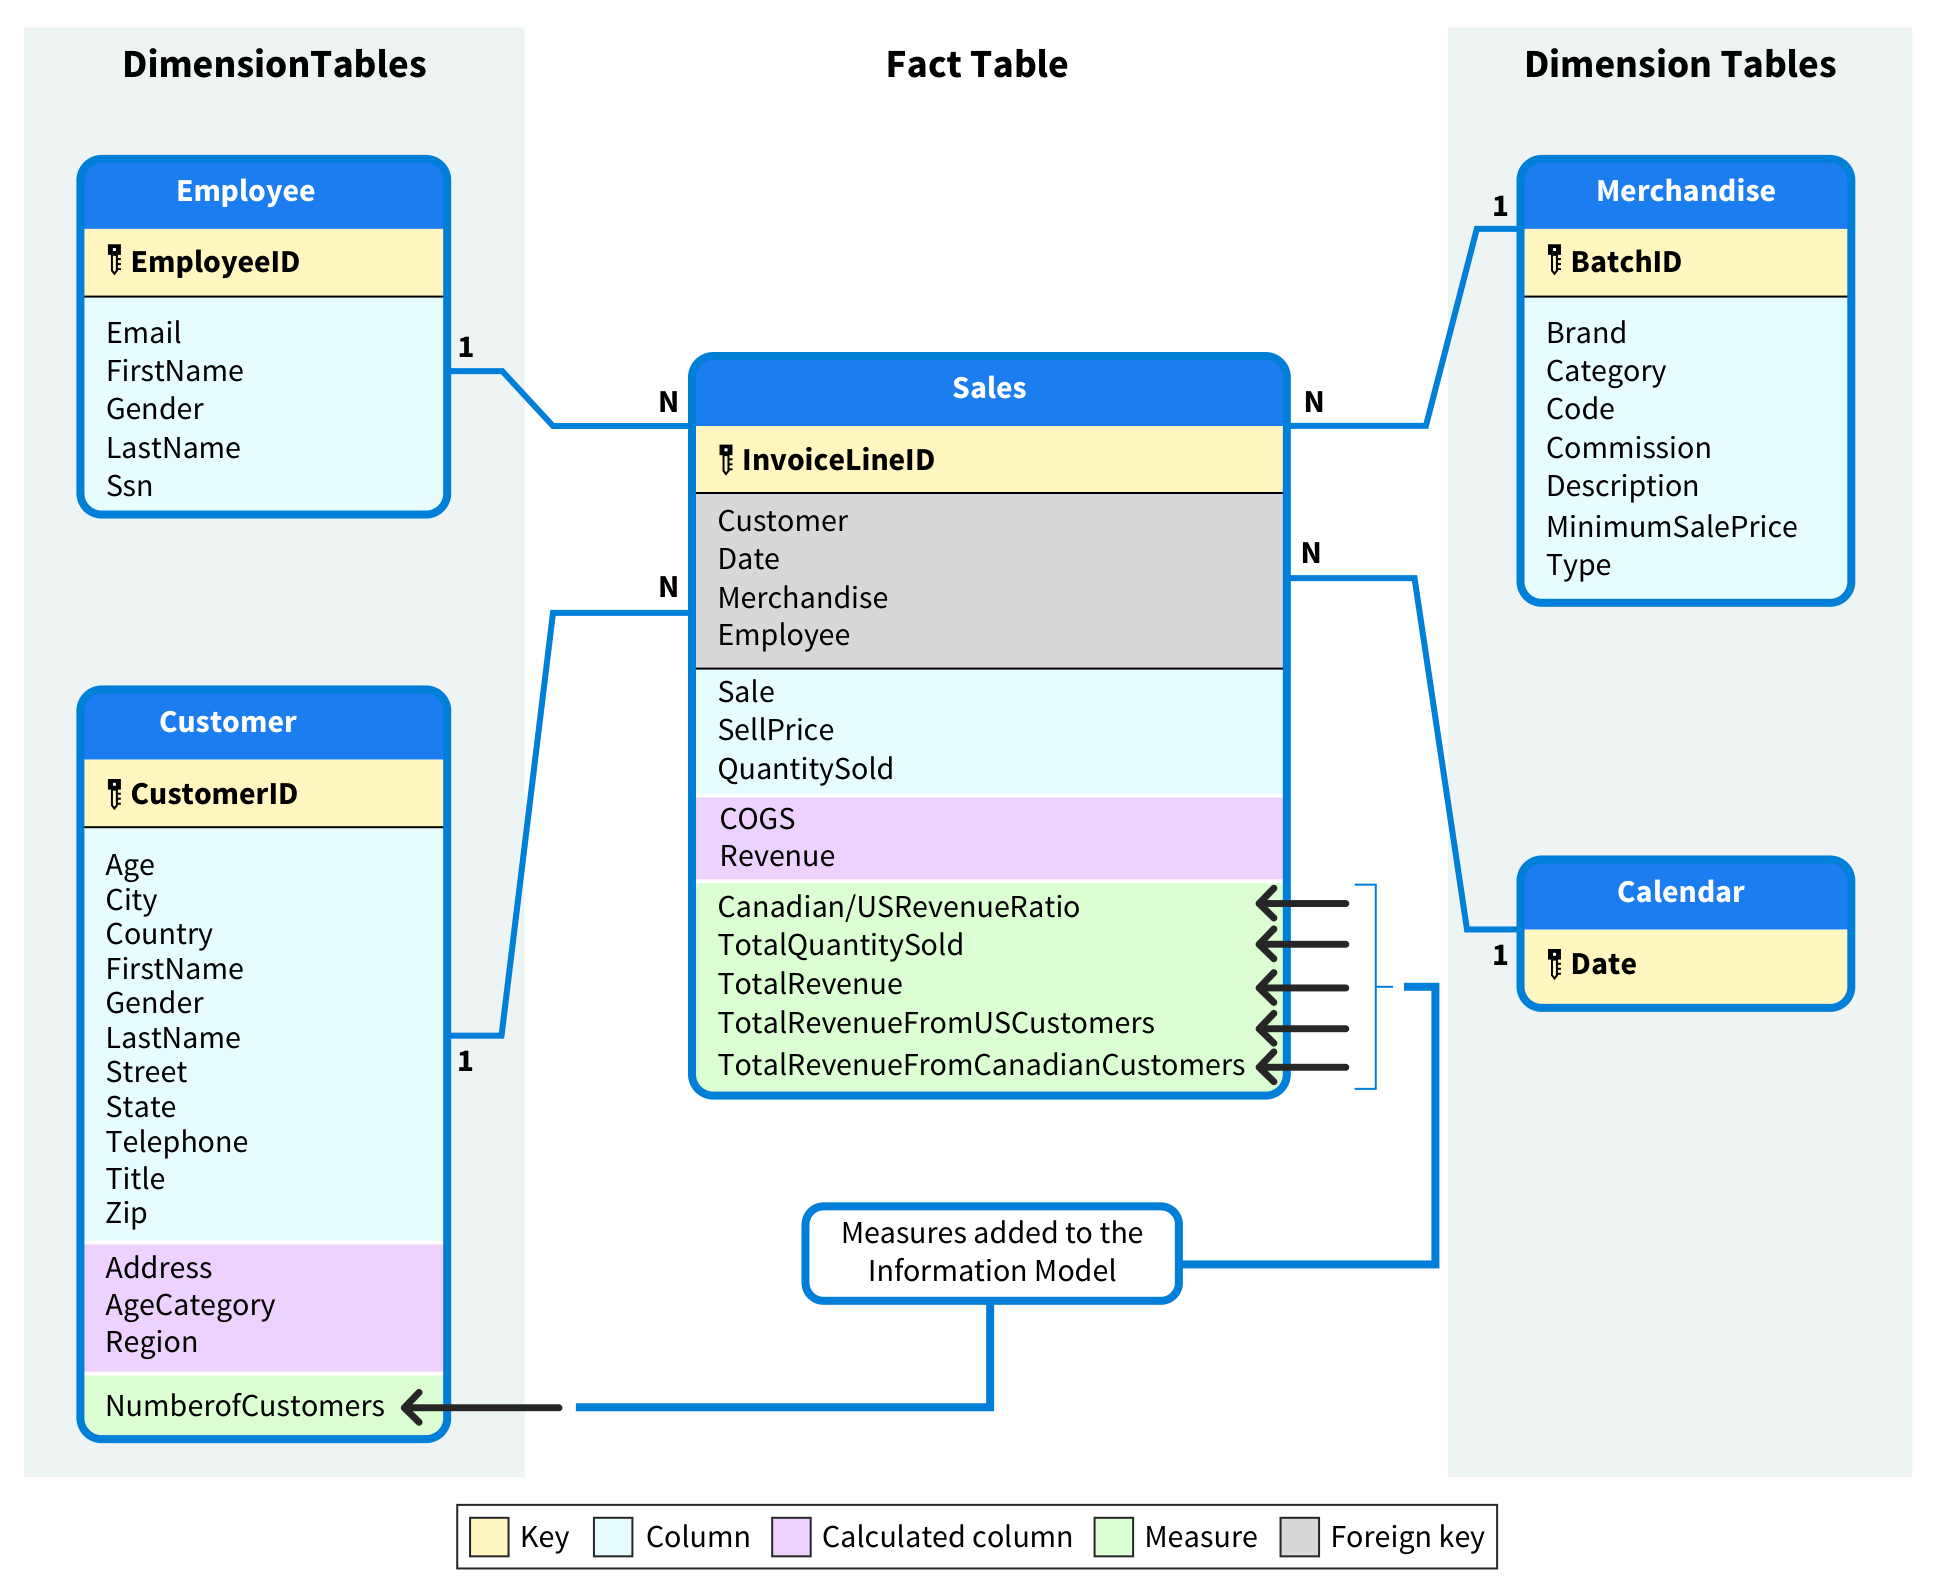
\includegraphics[width=0.95\textwidth,height=0.75\textheight,keepaspectratio]{../textbookForPractice/Figures/Ch_06/ILLUSTRATION 6.20.png}
    \end{figure}
\end{frame}

\begin{frame}{ILLUSTRATION 6.21}

    \begin{figure}[h]
        \centering
        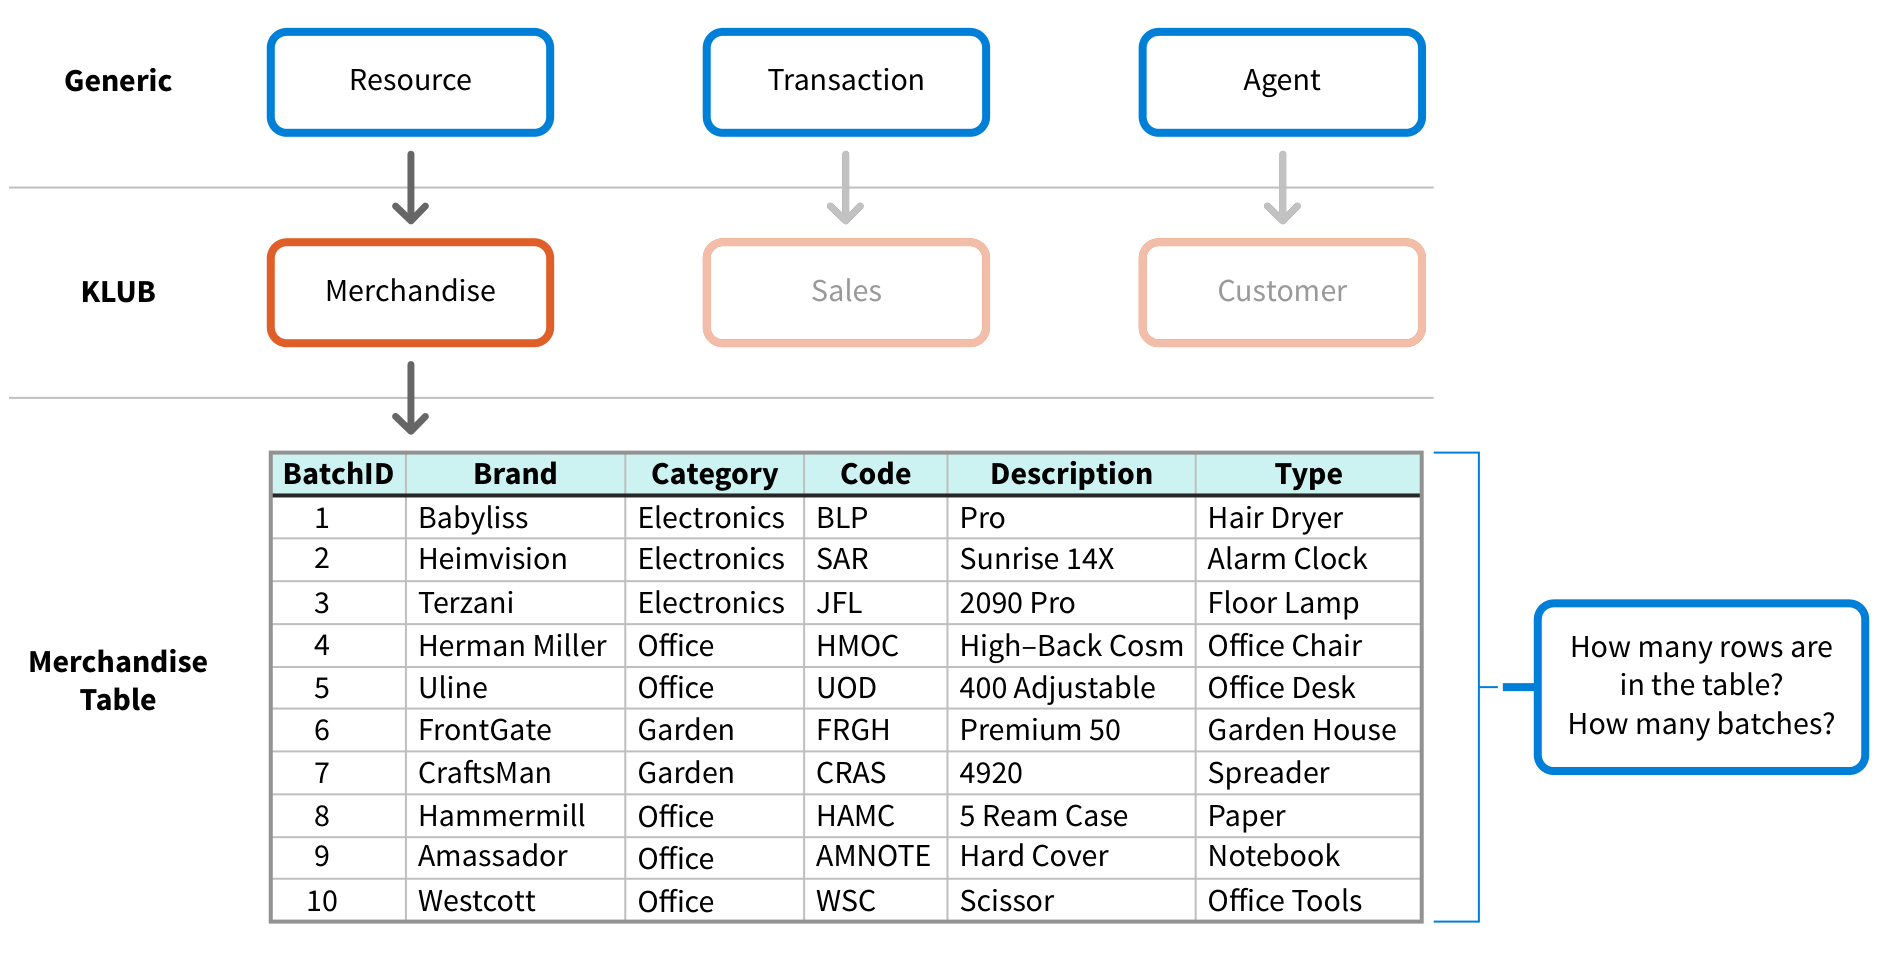
\includegraphics[width=0.95\textwidth,height=0.75\textheight,keepaspectratio]{../textbookForPractice/Figures/Ch_06/ILLUSTRATION 6.21.png}
    \end{figure}
\end{frame}

\begin{frame}{ILLUSTRATION 6.22}

    \begin{figure}[h]
        \centering
        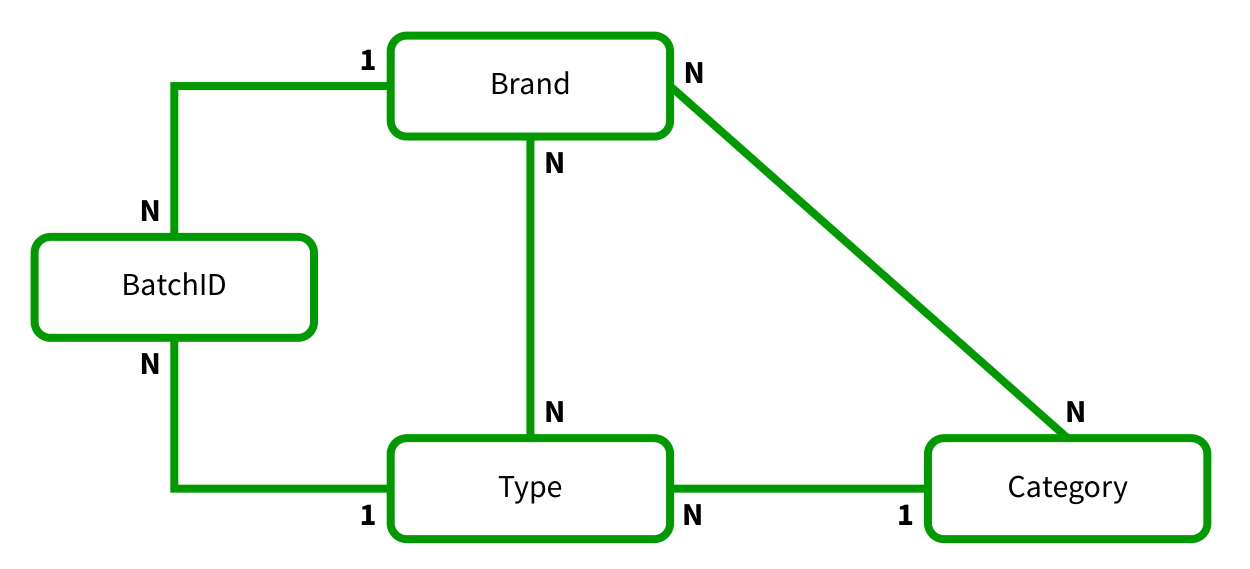
\includegraphics[width=0.95\textwidth,height=0.75\textheight,keepaspectratio]{../textbookForPractice/Figures/Ch_06/ILLUSTRATION 6.22.png}
    \end{figure}
\end{frame}

\begin{frame}{6.2 Bảy Mẫu Thuật toán Mô hình hóa Thông tin}
\begin{itemize}
    \item \textbf{Mẫu 1 - Tính toán Cơ bản:} Cộng, trừ, nhân, chia (ví dụ: Tổng Doanh thu).
    \item \textbf{Mẫu 2 - Logic và Điều kiện (Logic/Conditional):} Hàm IF, CASE WHEN (ví dụ: Phân loại Nợ xấu nếu quá hạn 90 ngày).
    \item \textbf{Mẫu 3 - Xử lý Văn bản (Text):} Nối chuỗi, tách chuỗi, làm sạch văn bản (ví dụ: Tách Mã Vùng từ Số Điện thoại).
\end{itemize}
\end{frame}

\begin{frame}{ILLUSTRATION 6.23}

    \begin{figure}[h]
        \centering
        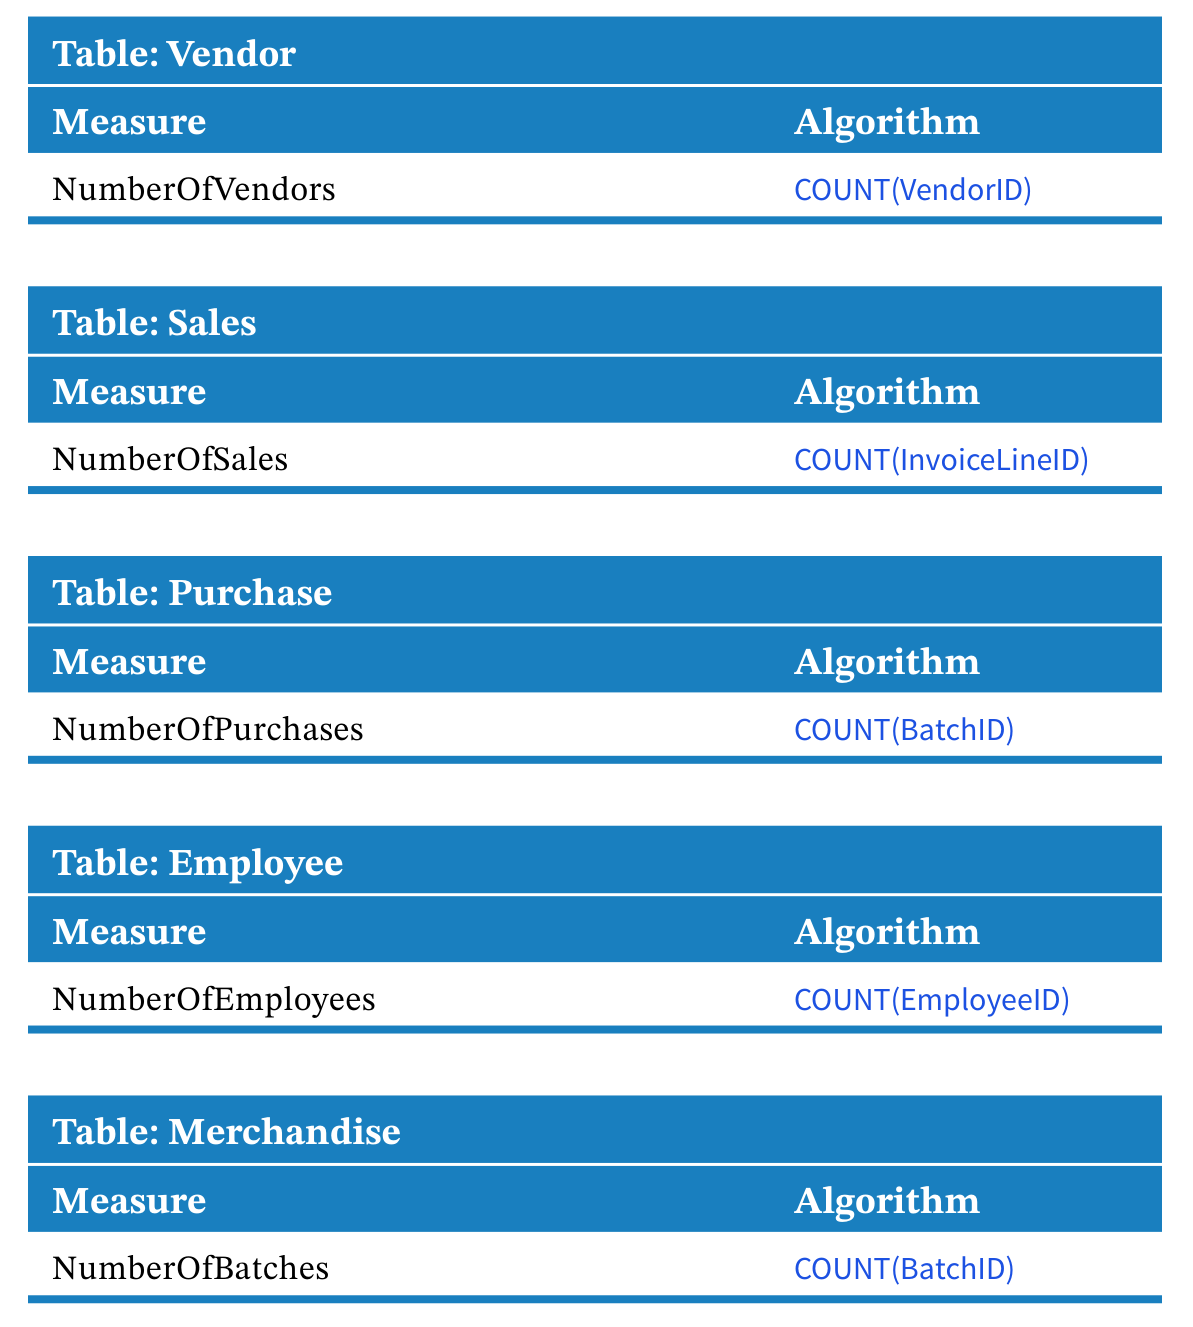
\includegraphics[width=0.95\textwidth,height=0.75\textheight,keepaspectratio]{../textbookForPractice/Figures/Ch_06/ILLUSTRATION 6.23.png}
    \end{figure}
\end{frame}

\begin{frame}{ILLUSTRATION 6.24}

    \begin{figure}[h]
        \centering
        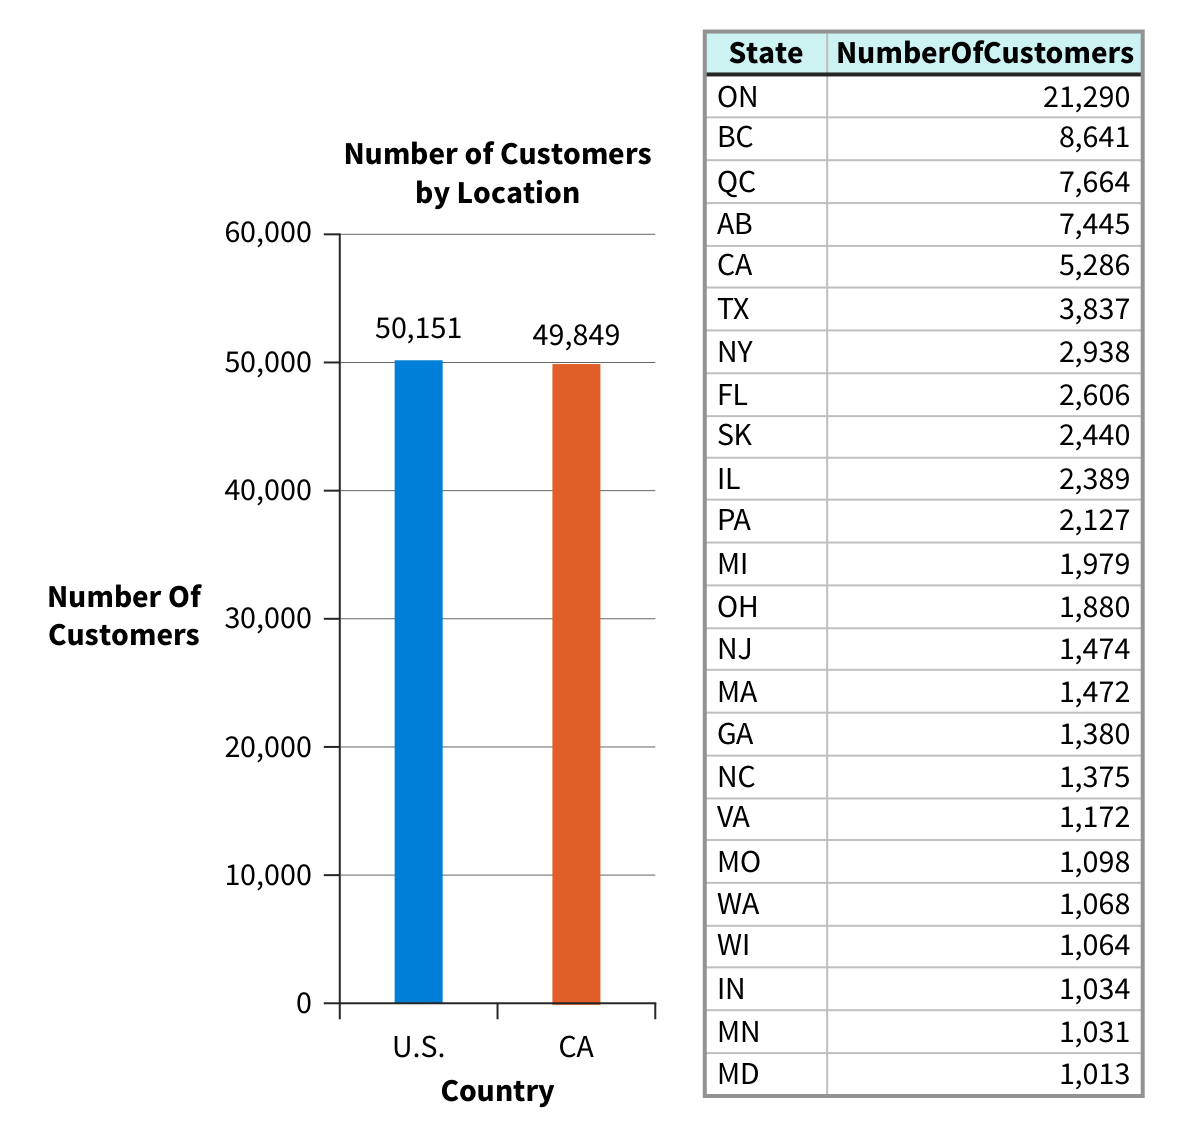
\includegraphics[width=0.95\textwidth,height=0.75\textheight,keepaspectratio]{../textbookForPractice/Figures/Ch_06/ILLUSTRATION 6.24.png}
    \end{figure}
\end{frame}

\begin{frame}{ILLUSTRATION 6.25}

    \begin{figure}[h]
        \centering
        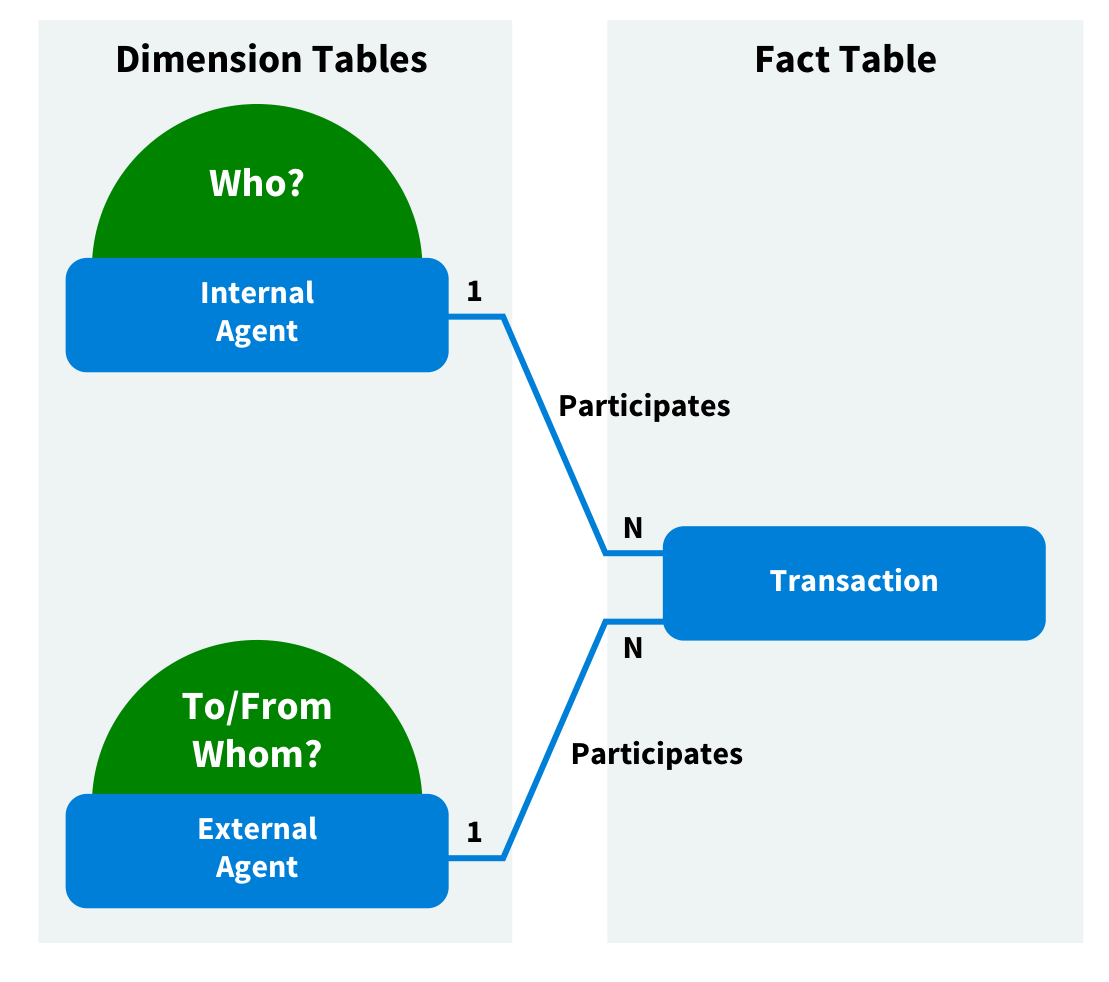
\includegraphics[width=0.95\textwidth,height=0.75\textheight,keepaspectratio]{../textbookForPractice/Figures/Ch_06/ILLUSTRATION 6.25.png}
    \end{figure}
\end{frame}

\begin{frame}{ILLUSTRATION 6.26}

    \begin{figure}[h]
        \centering
        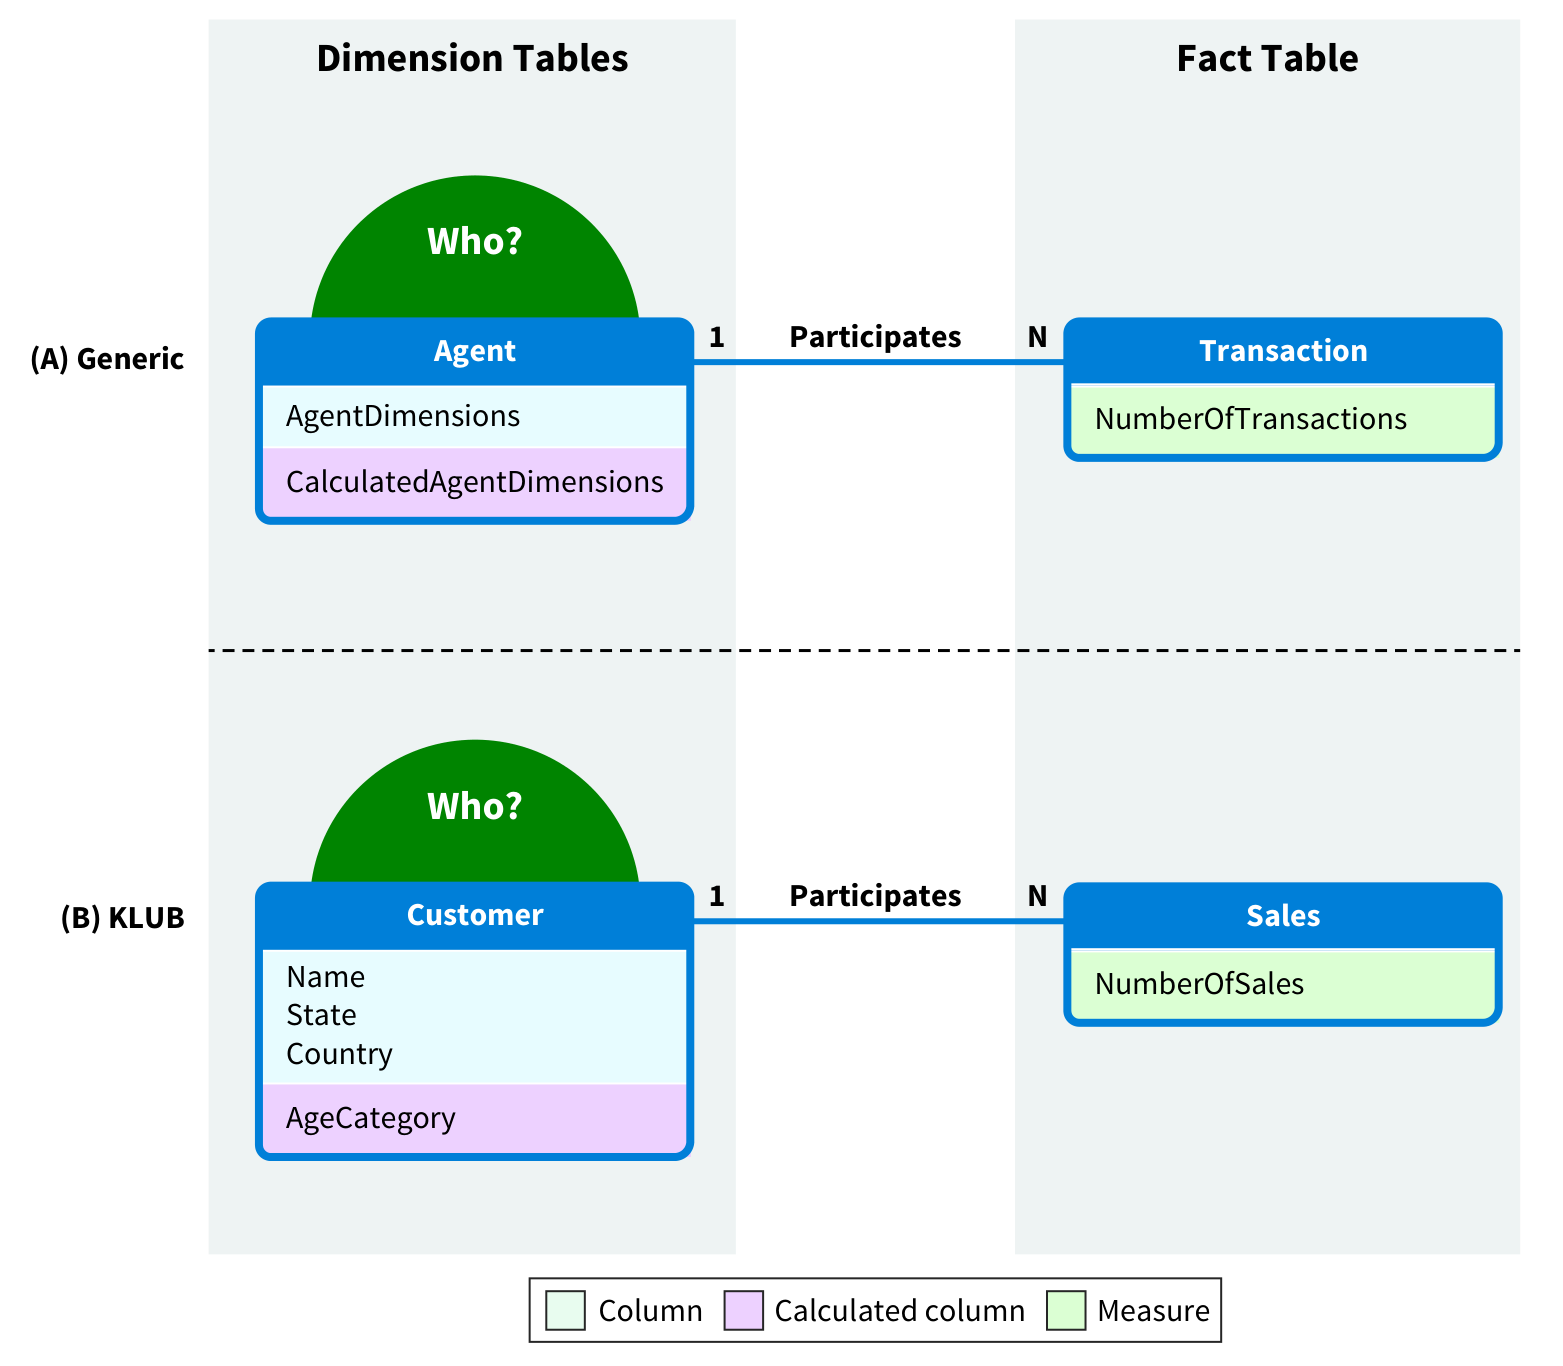
\includegraphics[width=0.95\textwidth,height=0.75\textheight,keepaspectratio]{../textbookForPractice/Figures/Ch_06/ILLUSTRATION 6.26.png}
    \end{figure}
\end{frame}

\begin{frame}{ILLUSTRATION 6.27}

    \begin{figure}[h]
        \centering
        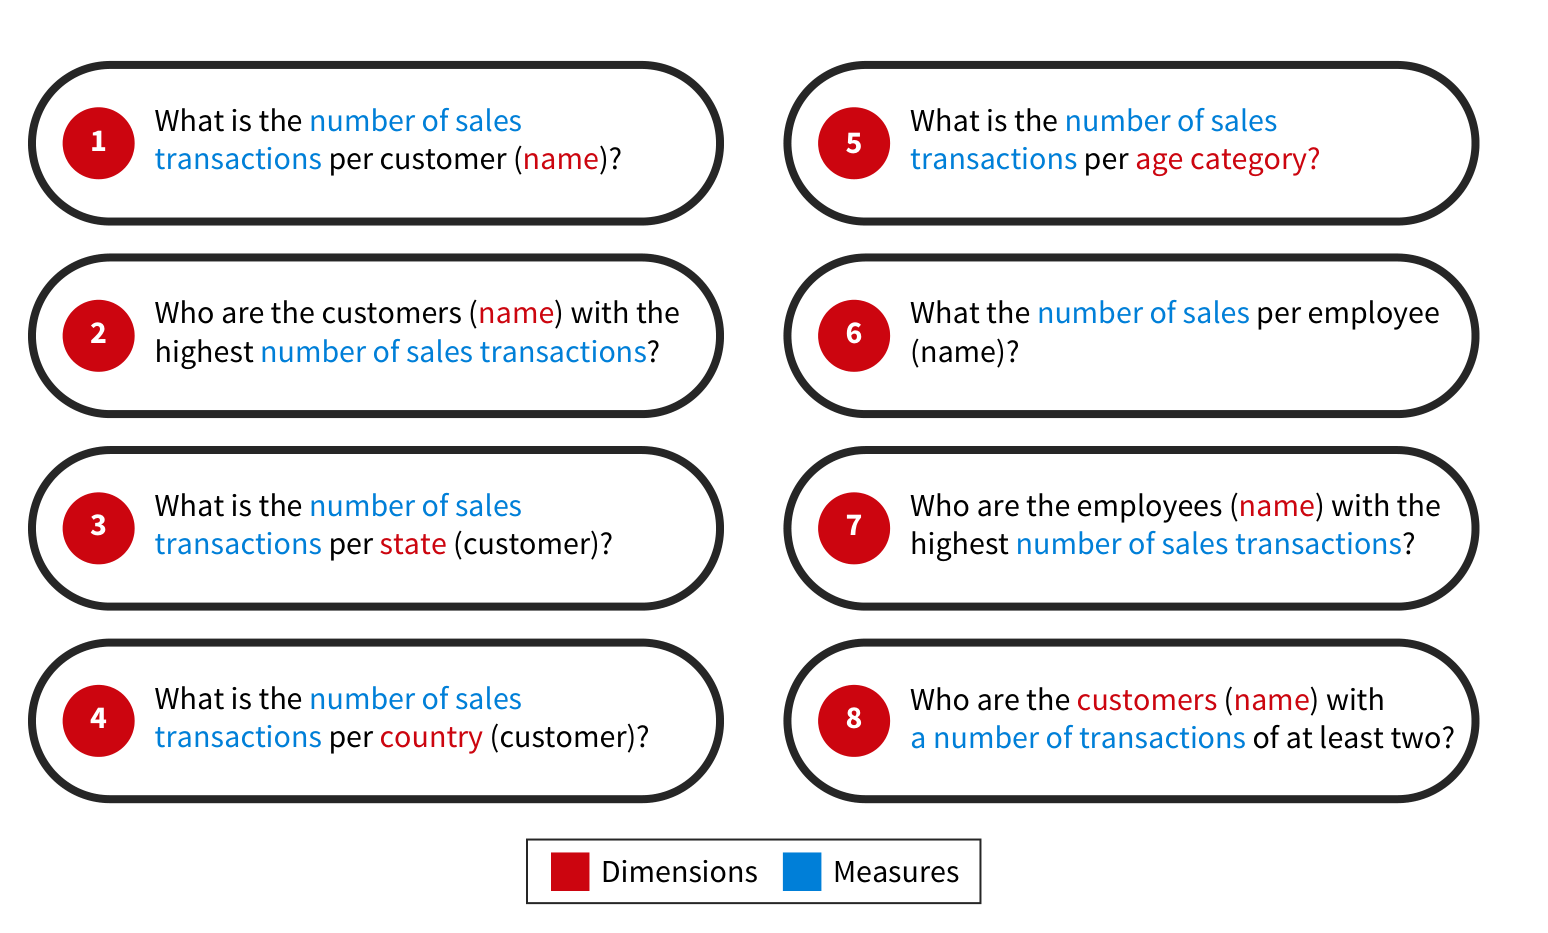
\includegraphics[width=0.95\textwidth,height=0.75\textheight,keepaspectratio]{../textbookForPractice/Figures/Ch_06/ILLUSTRATION 6.27.png}
    \end{figure}
\end{frame}

\begin{frame}{ILLUSTRATION 6.28}

    \begin{figure}[h]
        \centering
        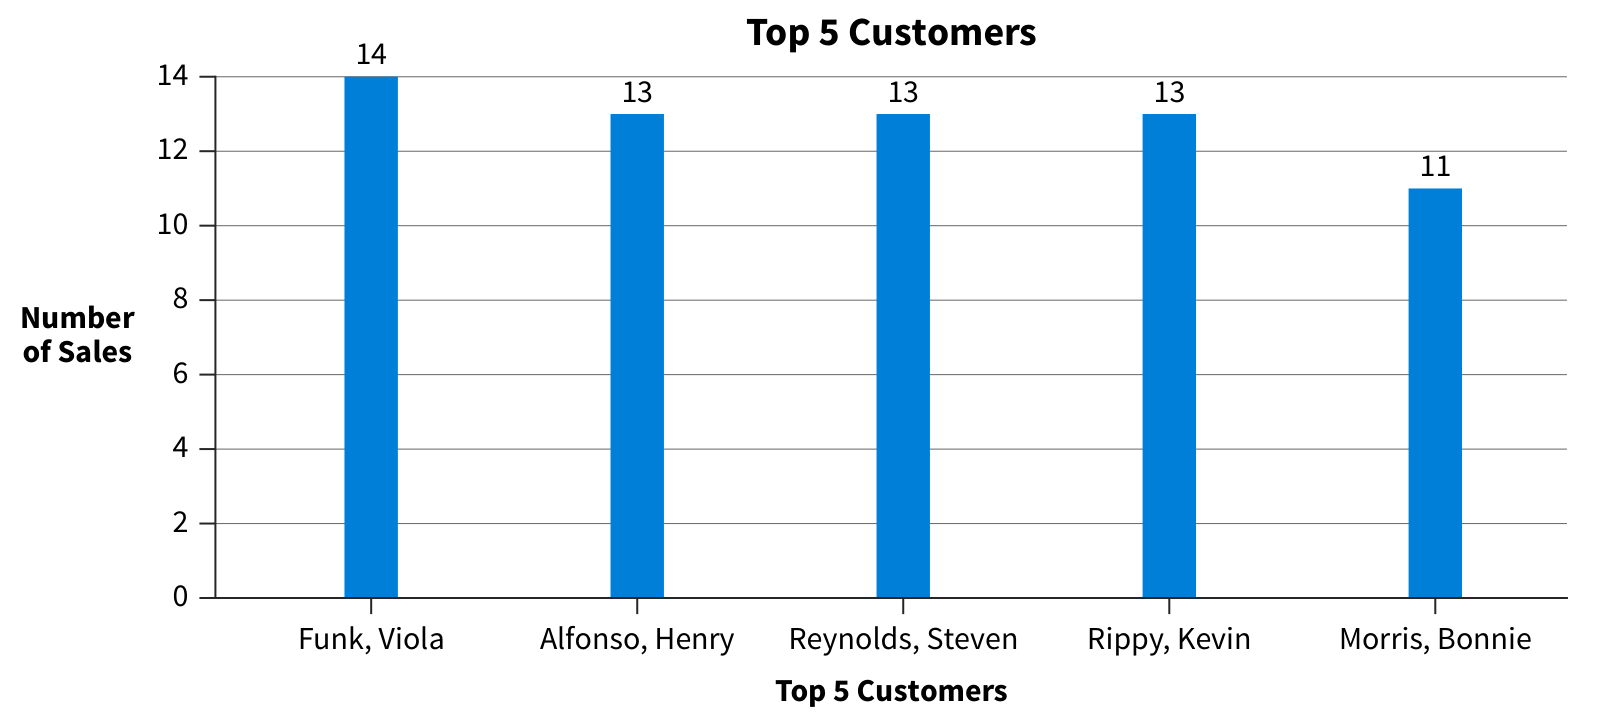
\includegraphics[width=0.95\textwidth,height=0.75\textheight,keepaspectratio]{../textbookForPractice/Figures/Ch_06/ILLUSTRATION 6.28.png}
    \end{figure}
\end{frame}

\begin{frame}{ILLUSTRATION 6.29}

    \begin{figure}[h]
        \centering
        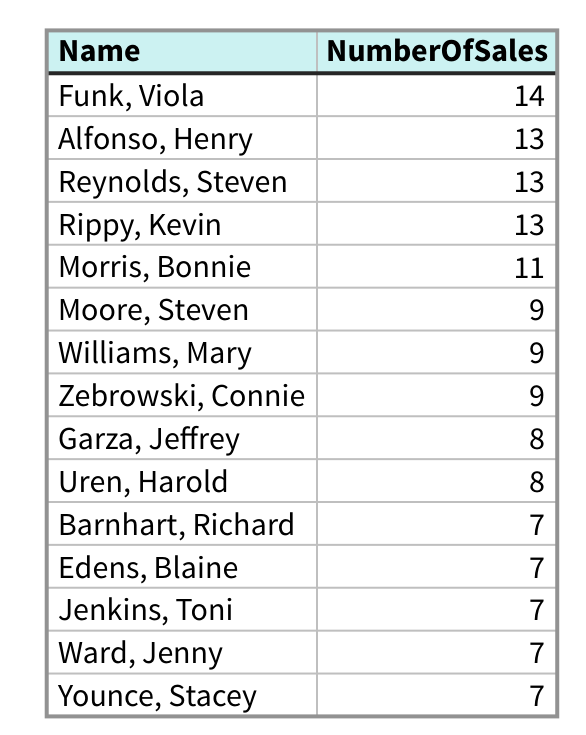
\includegraphics[width=0.95\textwidth,height=0.75\textheight,keepaspectratio]{../textbookForPractice/Figures/Ch_06/ILLUSTRATION 6.29.png}
    \end{figure}
\end{frame}

\begin{frame}{ILLUSTRATION 6.30}

    \begin{figure}[h]
        \centering
        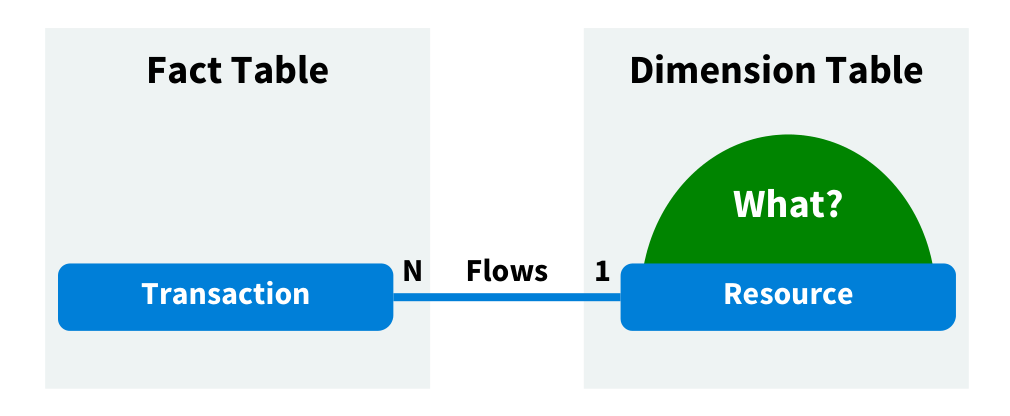
\includegraphics[width=0.95\textwidth,height=0.75\textheight,keepaspectratio]{../textbookForPractice/Figures/Ch_06/ILLUSTRATION 6.30.png}
    \end{figure}
\end{frame}

\begin{frame}{ILLUSTRATION 6.31}

    \begin{figure}[h]
        \centering
        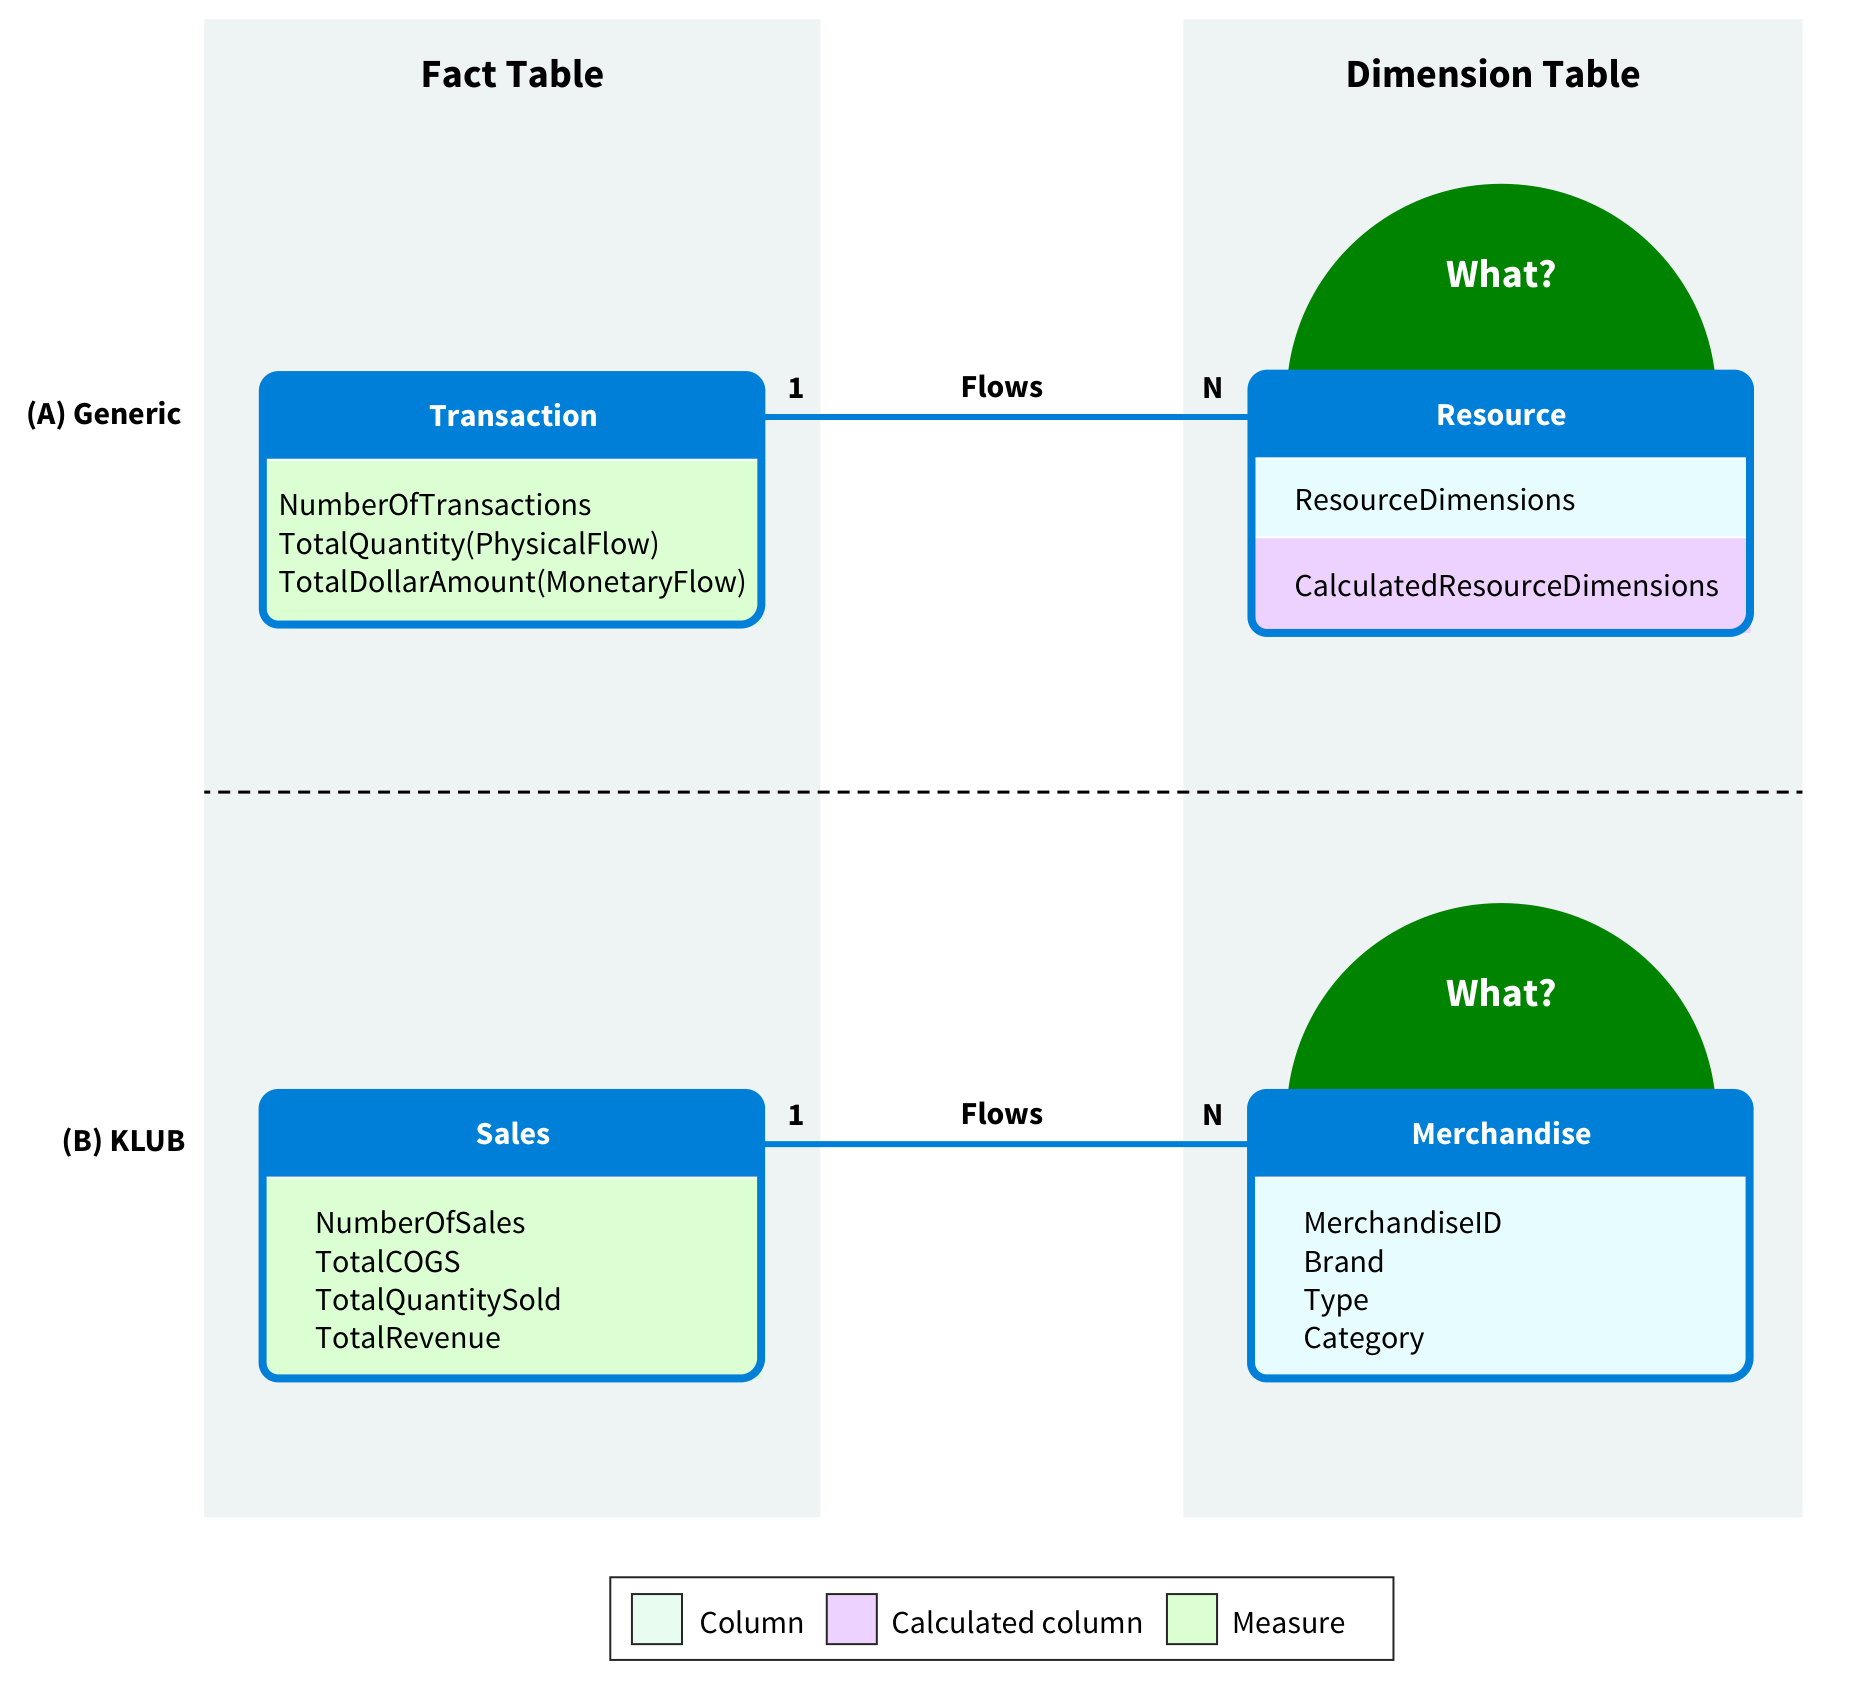
\includegraphics[width=0.95\textwidth,height=0.75\textheight,keepaspectratio]{../textbookForPractice/Figures/Ch_06/ILLUSTRATION 6.31.png}
    \end{figure}
\end{frame}

\begin{frame}{ILLUSTRATION 6.32}

    \begin{figure}[h]
        \centering
        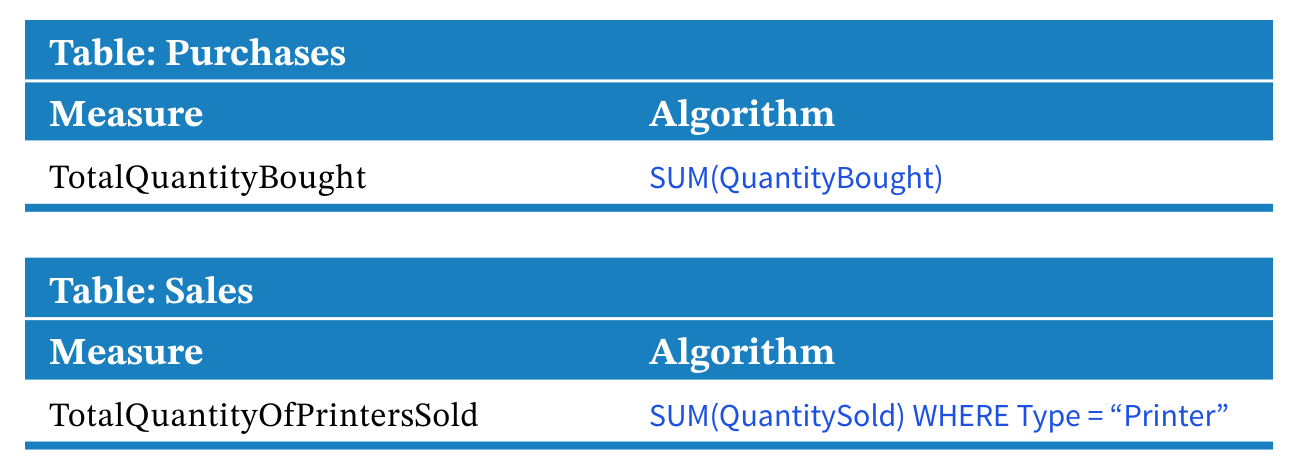
\includegraphics[width=0.95\textwidth,height=0.75\textheight,keepaspectratio]{../textbookForPractice/Figures/Ch_06/ILLUSTRATION 6.32.png}
    \end{figure}
\end{frame}

\begin{frame}{ILLUSTRATION 6.33}

    \begin{figure}[h]
        \centering
        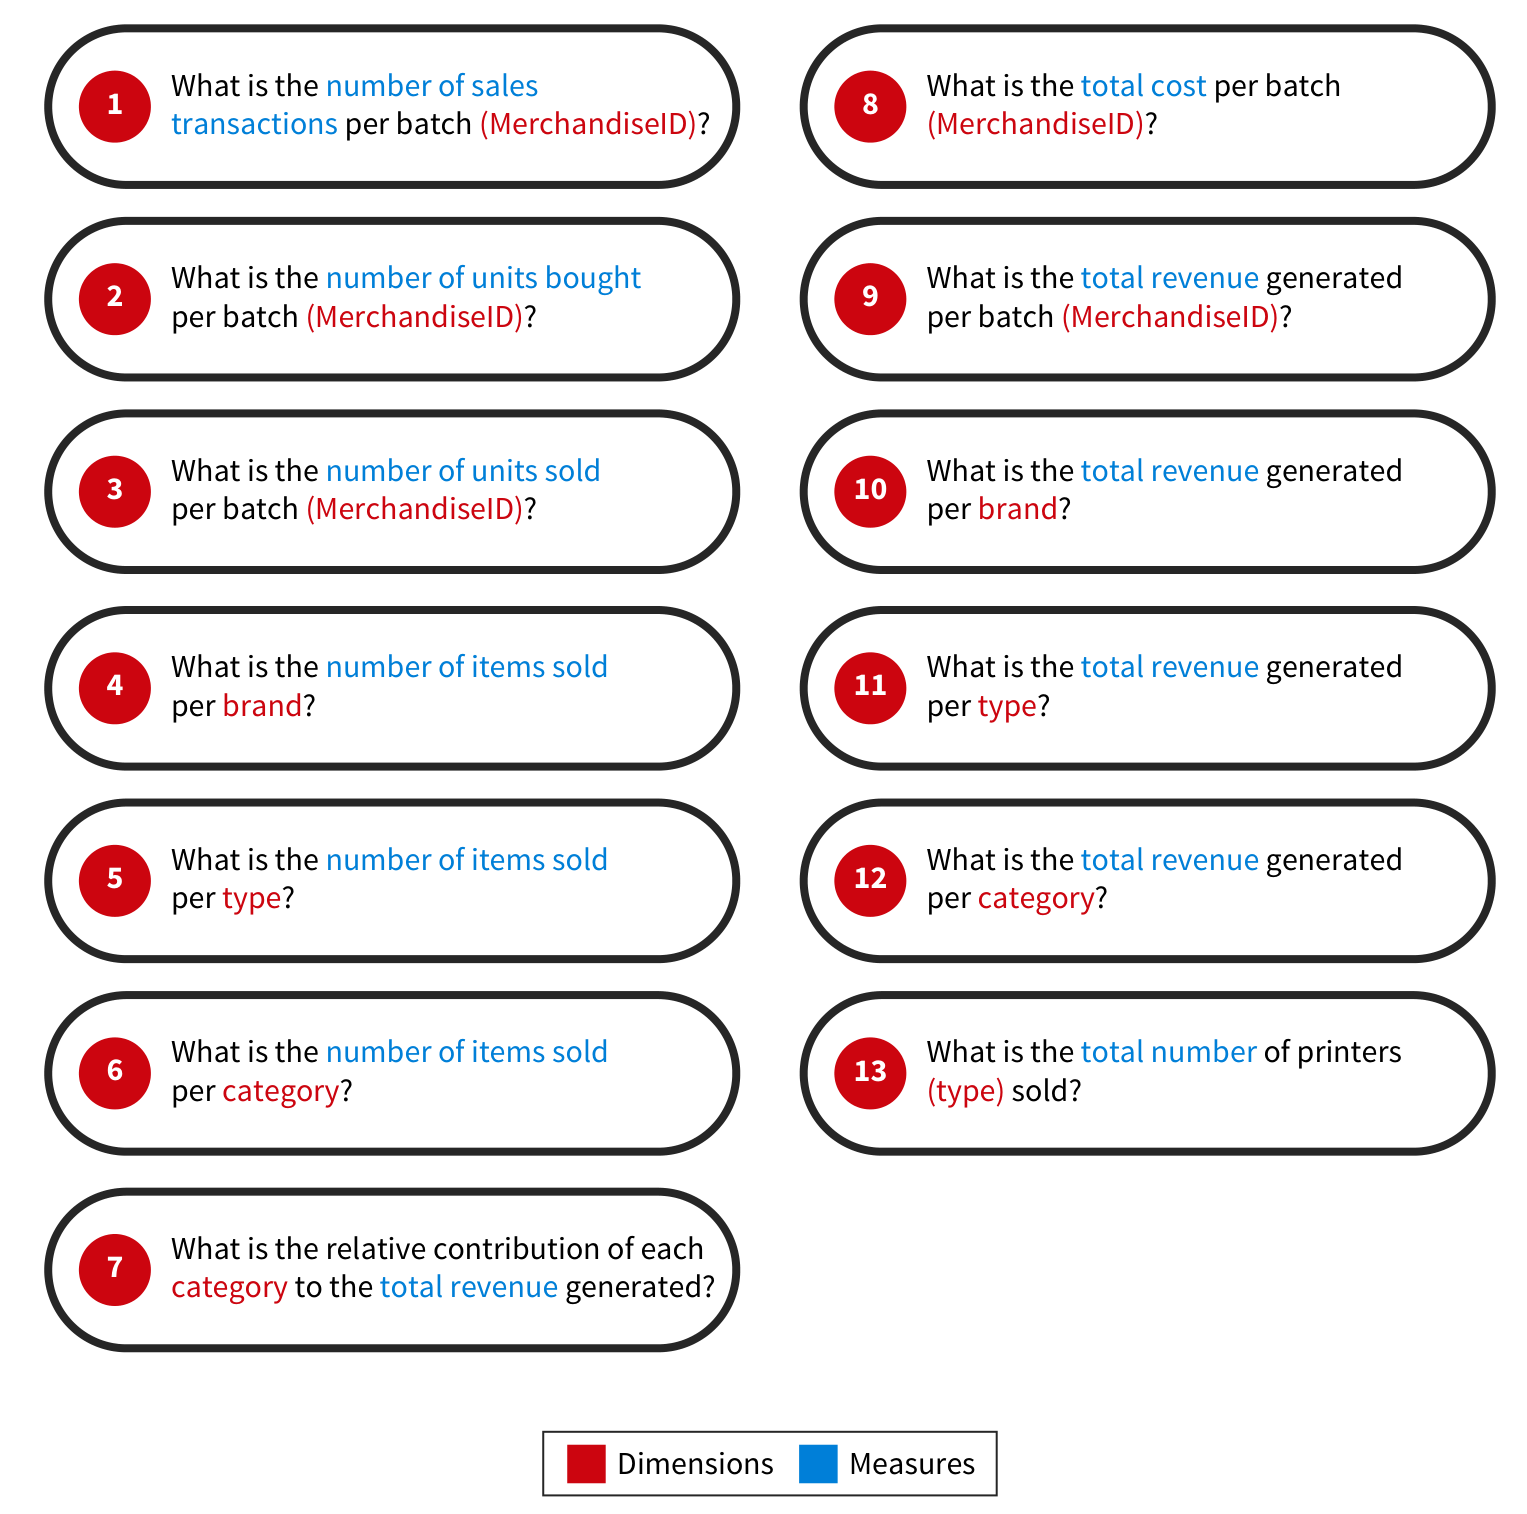
\includegraphics[width=0.95\textwidth,height=0.75\textheight,keepaspectratio]{../textbookForPractice/Figures/Ch_06/ILLUSTRATION 6.33.png}
    \end{figure}
\end{frame}

\begin{frame}{Các Mẫu Thuật toán tiếp theo}
\begin{itemize}
    \item \textbf{Mẫu 4 - Thời gian (Date/Time):} Trích xuất Tháng, Năm, Quý (ví dụ: Doanh thu theo Quý).
    \item \textbf{Mẫu 5 - Hàm Tài chính (Financial):} Tính PV, FV, NPV, IRR.
    \item \textbf{Mẫu 6 - Tỷ suất (Ratios):} Tính ROA, ROE, Current Ratio.
    \item \textbf{Mẫu 7 - Hàm Phức hợp (Complex/Nested):} Kết hợp nhiều hàm với nhau.
\end{itemize}
\end{frame}

\begin{frame}{ILLUSTRATION 6.34}

    \begin{figure}[h]
        \centering
        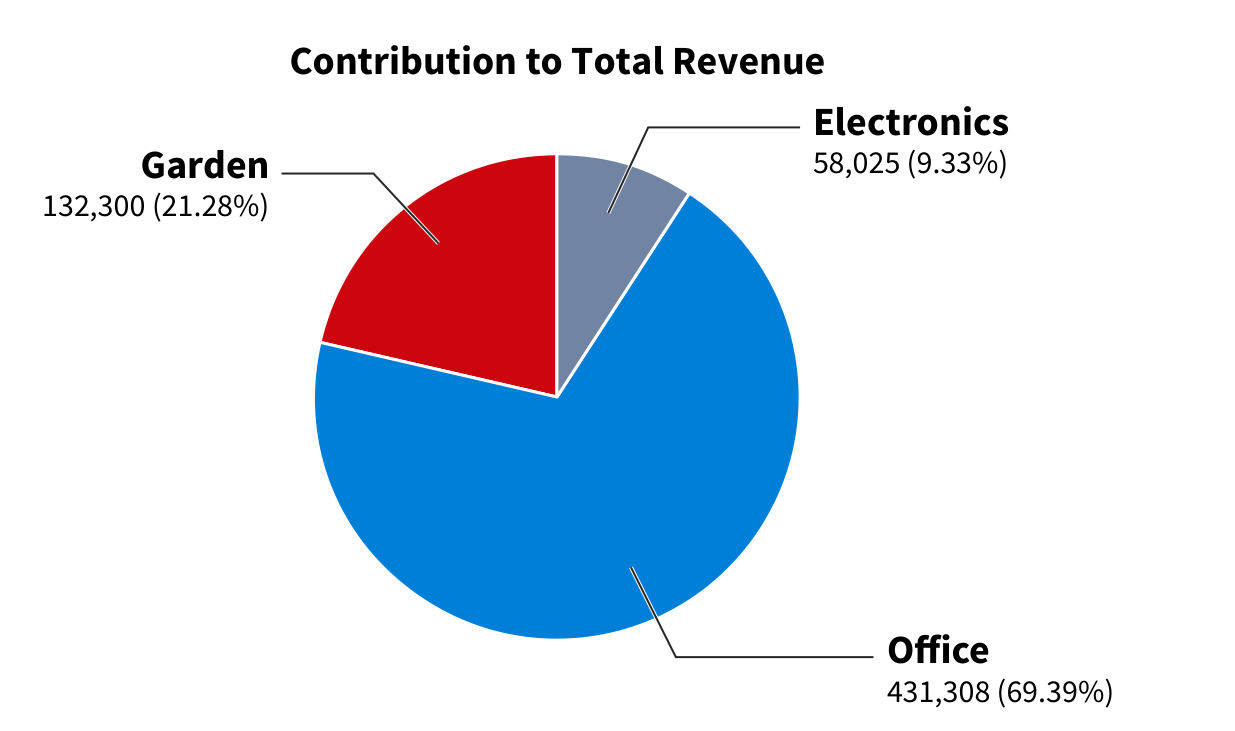
\includegraphics[width=0.95\textwidth,height=0.75\textheight,keepaspectratio]{../textbookForPractice/Figures/Ch_06/ILLUSTRATION 6.34.png}
    \end{figure}
\end{frame}

\begin{frame}{ILLUSTRATION 6.35}

    \begin{figure}[h]
        \centering
        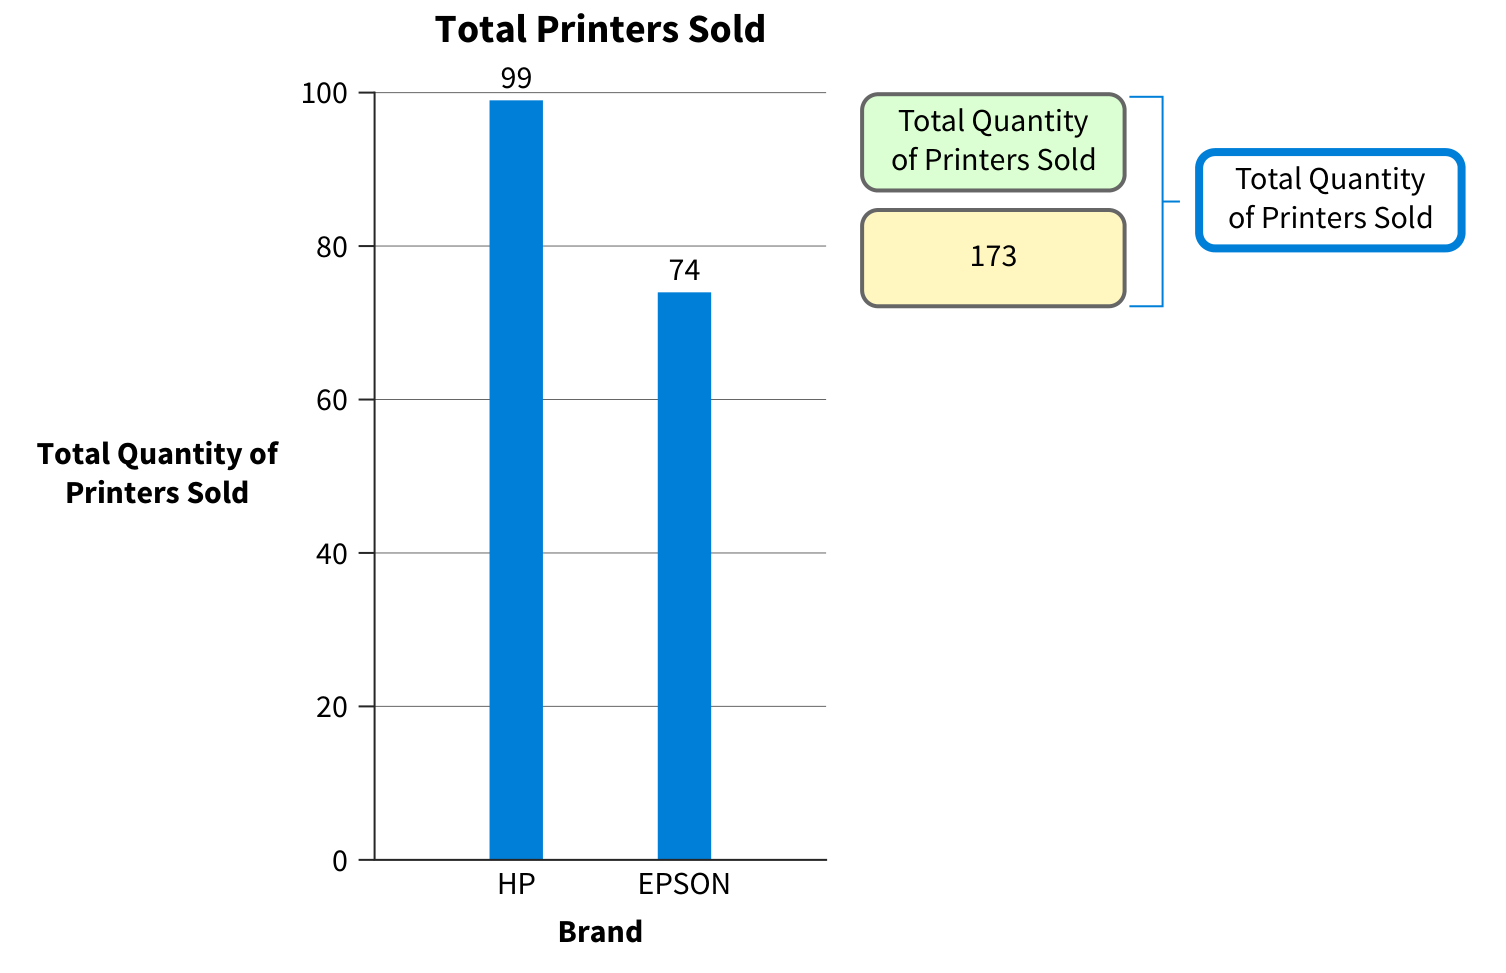
\includegraphics[width=0.95\textwidth,height=0.75\textheight,keepaspectratio]{../textbookForPractice/Figures/Ch_06/ILLUSTRATION 6.35.png}
    \end{figure}
\end{frame}

\begin{frame}{ILLUSTRATION 6.36}

    \begin{figure}[h]
        \centering
        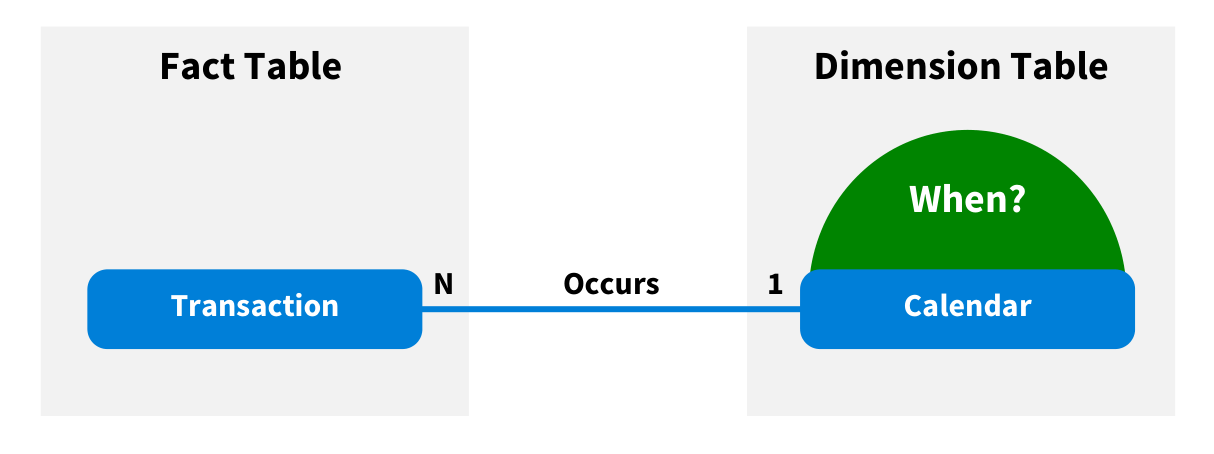
\includegraphics[width=0.95\textwidth,height=0.75\textheight,keepaspectratio]{../textbookForPractice/Figures/Ch_06/ILLUSTRATION 6.36.png}
    \end{figure}
\end{frame}

\begin{frame}{ILLUSTRATION 6.37}

    \begin{figure}[h]
        \centering
        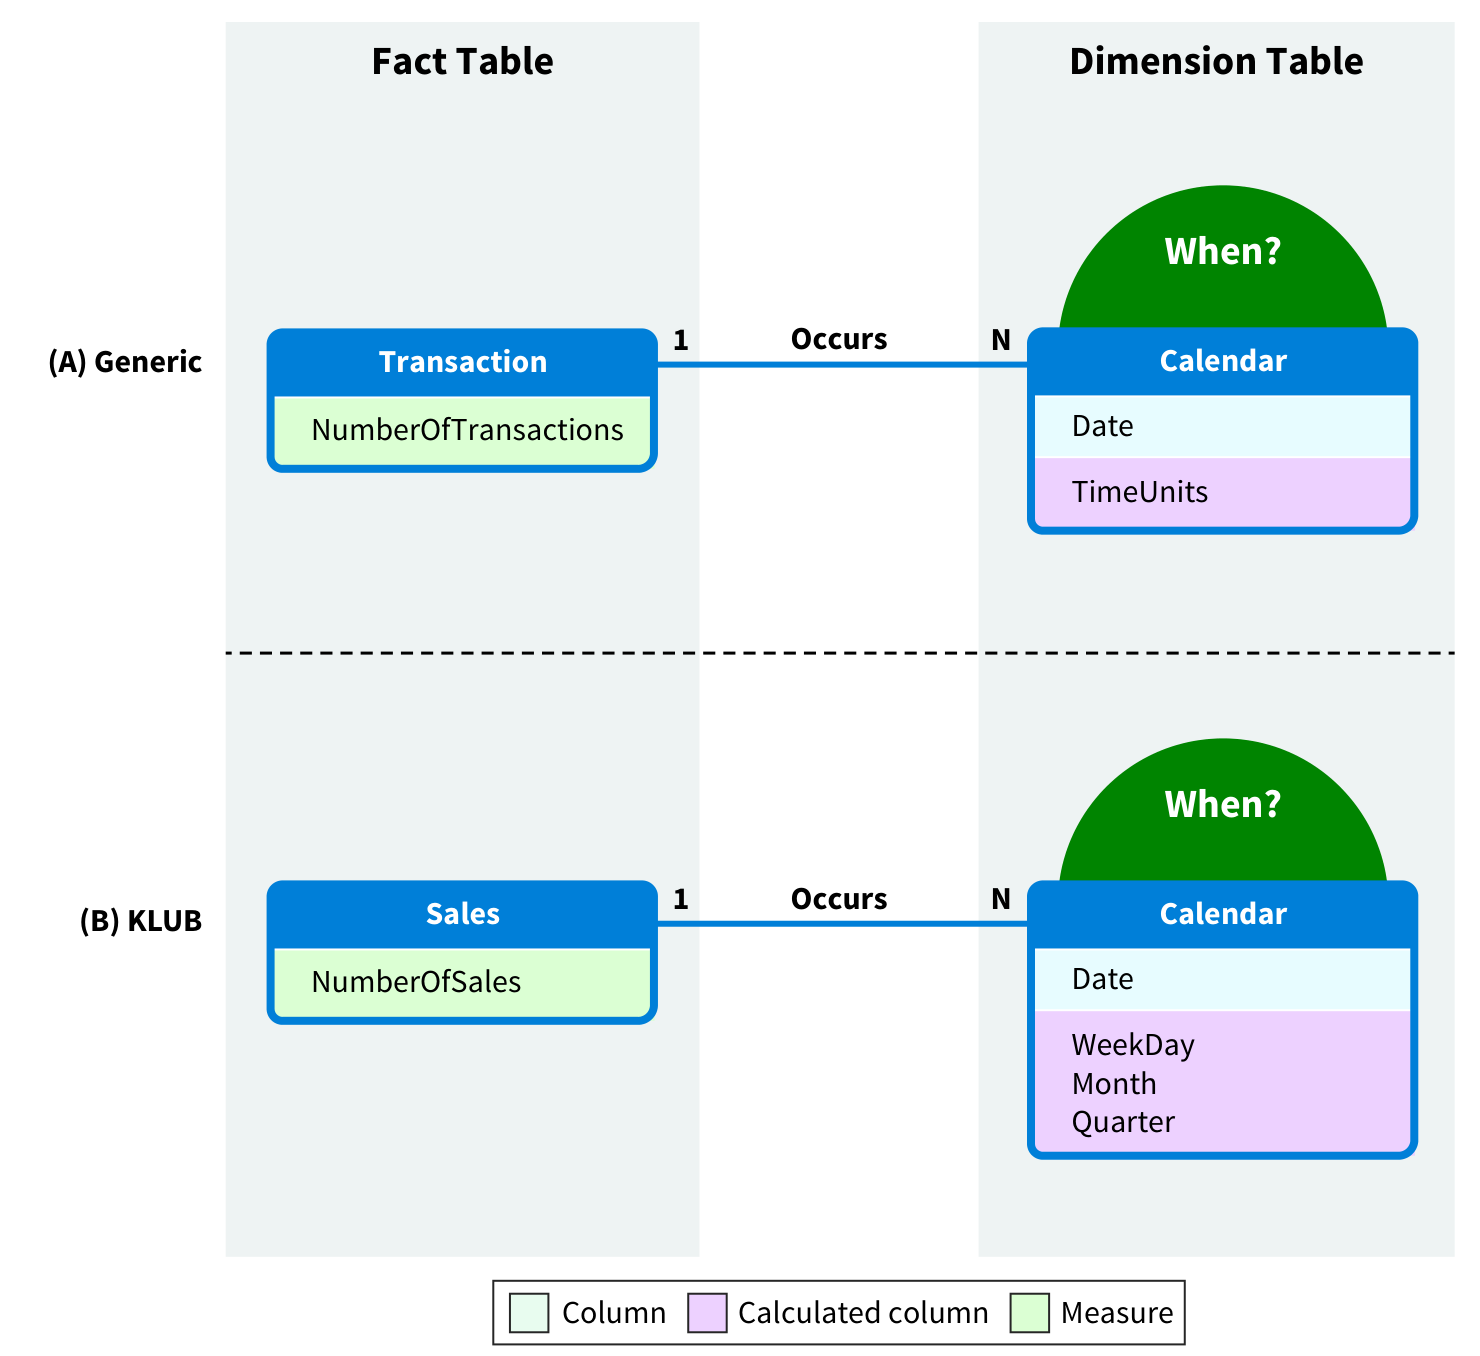
\includegraphics[width=0.95\textwidth,height=0.75\textheight,keepaspectratio]{../textbookForPractice/Figures/Ch_06/ILLUSTRATION 6.37.png}
    \end{figure}
\end{frame}

\begin{frame}{ILLUSTRATION 6.38}

    \begin{figure}[h]
        \centering
        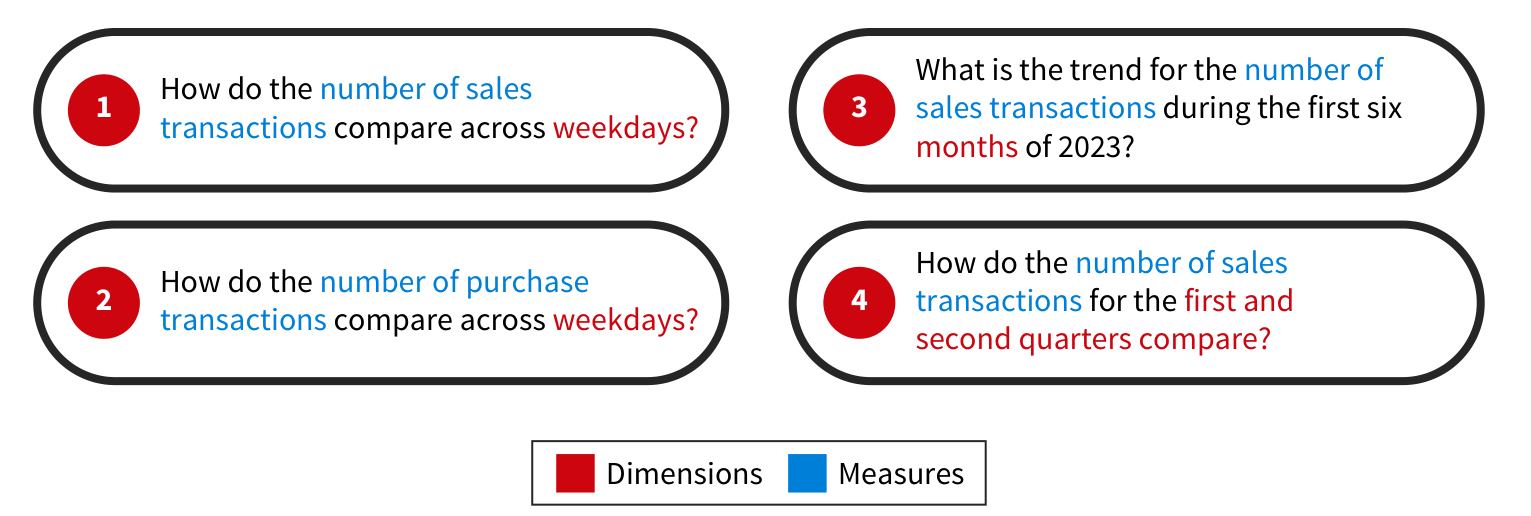
\includegraphics[width=0.95\textwidth,height=0.75\textheight,keepaspectratio]{../textbookForPractice/Figures/Ch_06/ILLUSTRATION 6.38.png}
    \end{figure}
\end{frame}

\begin{frame}{ILLUSTRATION 6.39}

    \begin{figure}[h]
        \centering
        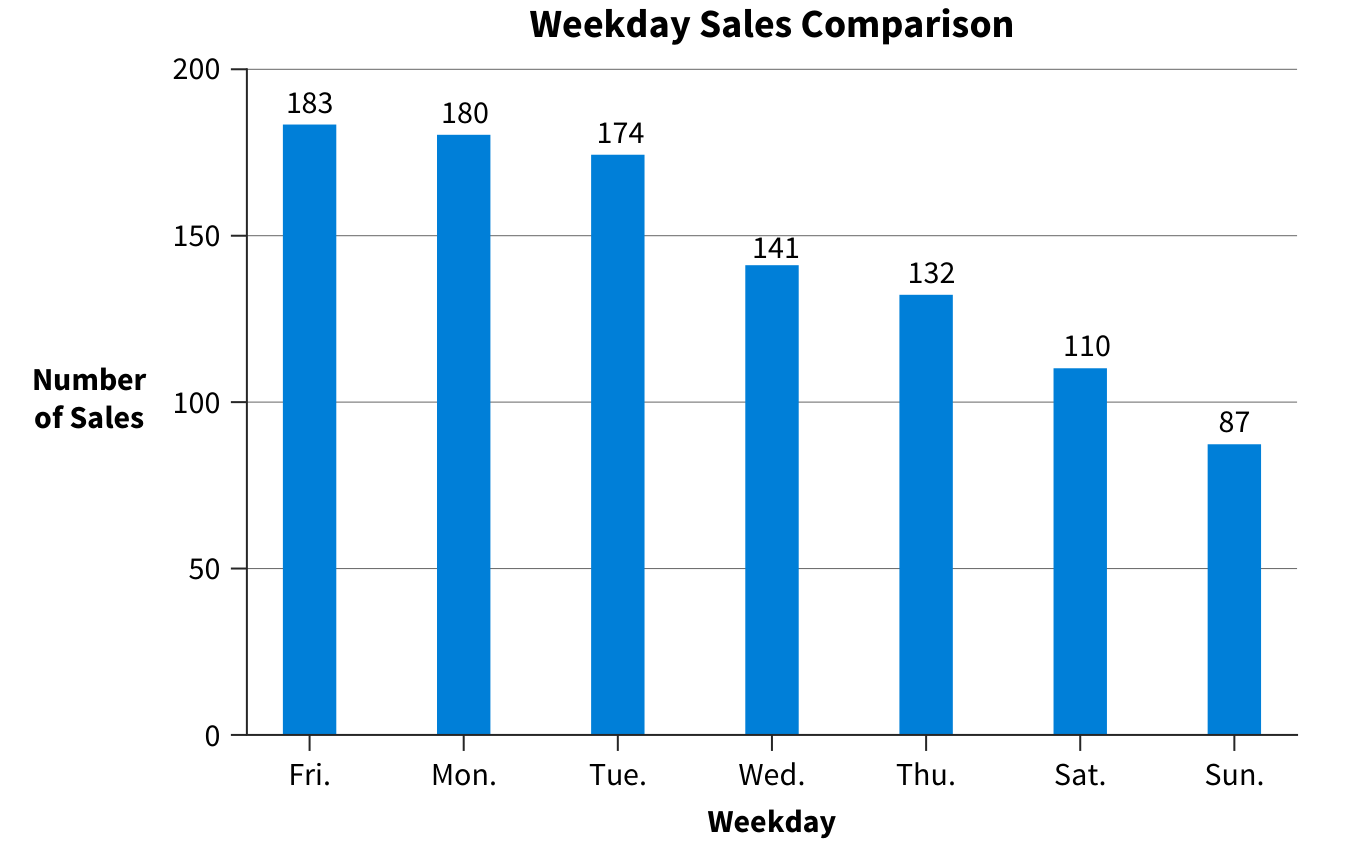
\includegraphics[width=0.95\textwidth,height=0.75\textheight,keepaspectratio]{../textbookForPractice/Figures/Ch_06/ILLUSTRATION 6.39.png}
    \end{figure}
\end{frame}

\begin{frame}{ILLUSTRATION 6.40}

    \begin{figure}[h]
        \centering
        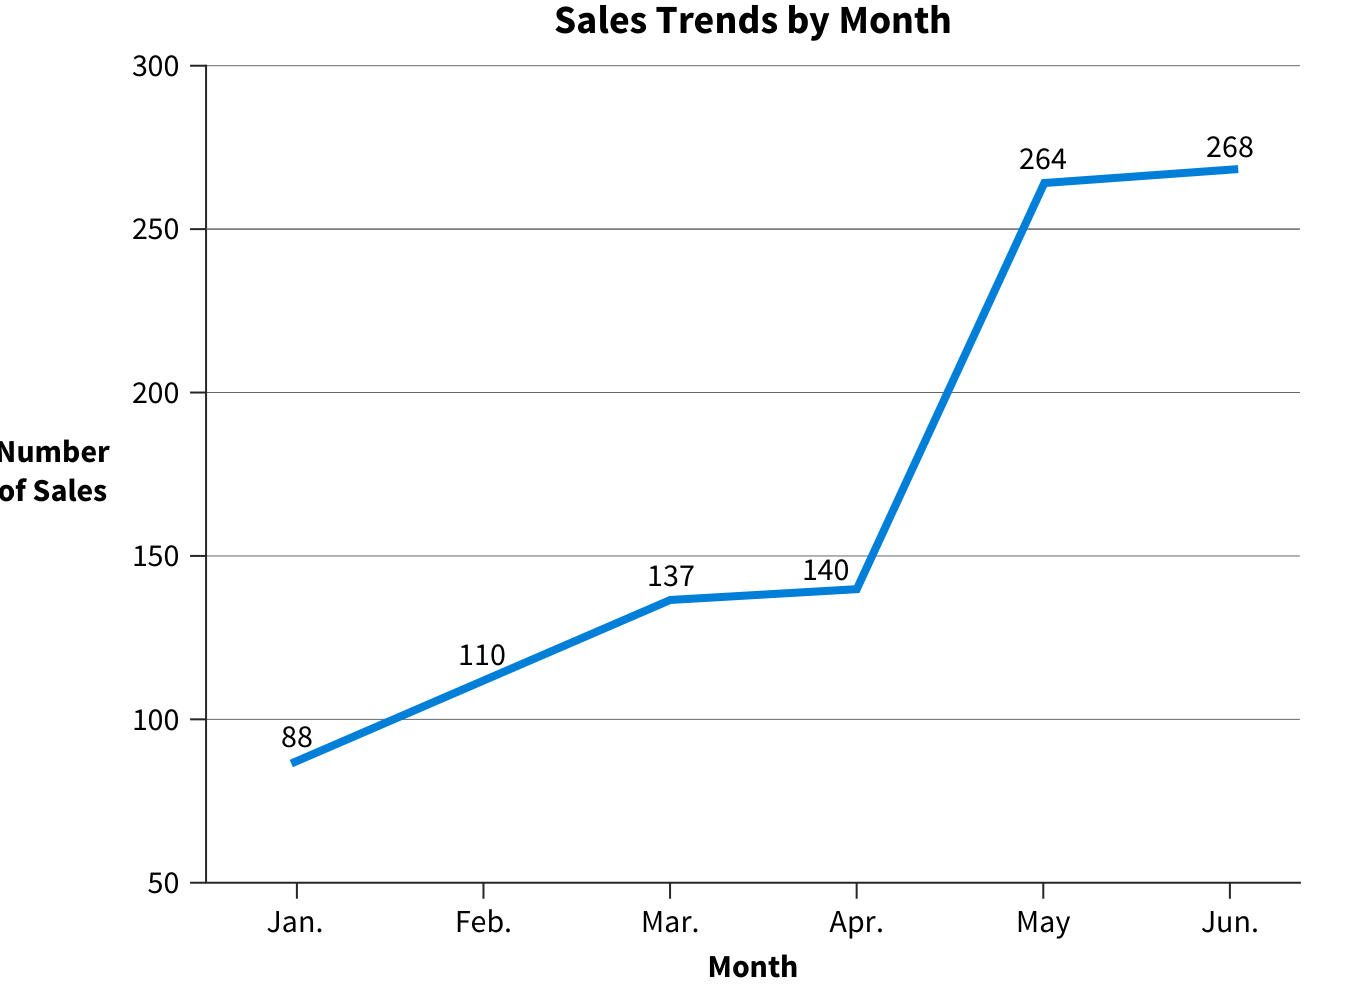
\includegraphics[width=0.95\textwidth,height=0.75\textheight,keepaspectratio]{../textbookForPractice/Figures/Ch_06/ILLUSTRATION 6.40.png}
    \end{figure}
\end{frame}

\begin{frame}{ILLUSTRATION 6.41}

    \begin{figure}[h]
        \centering
        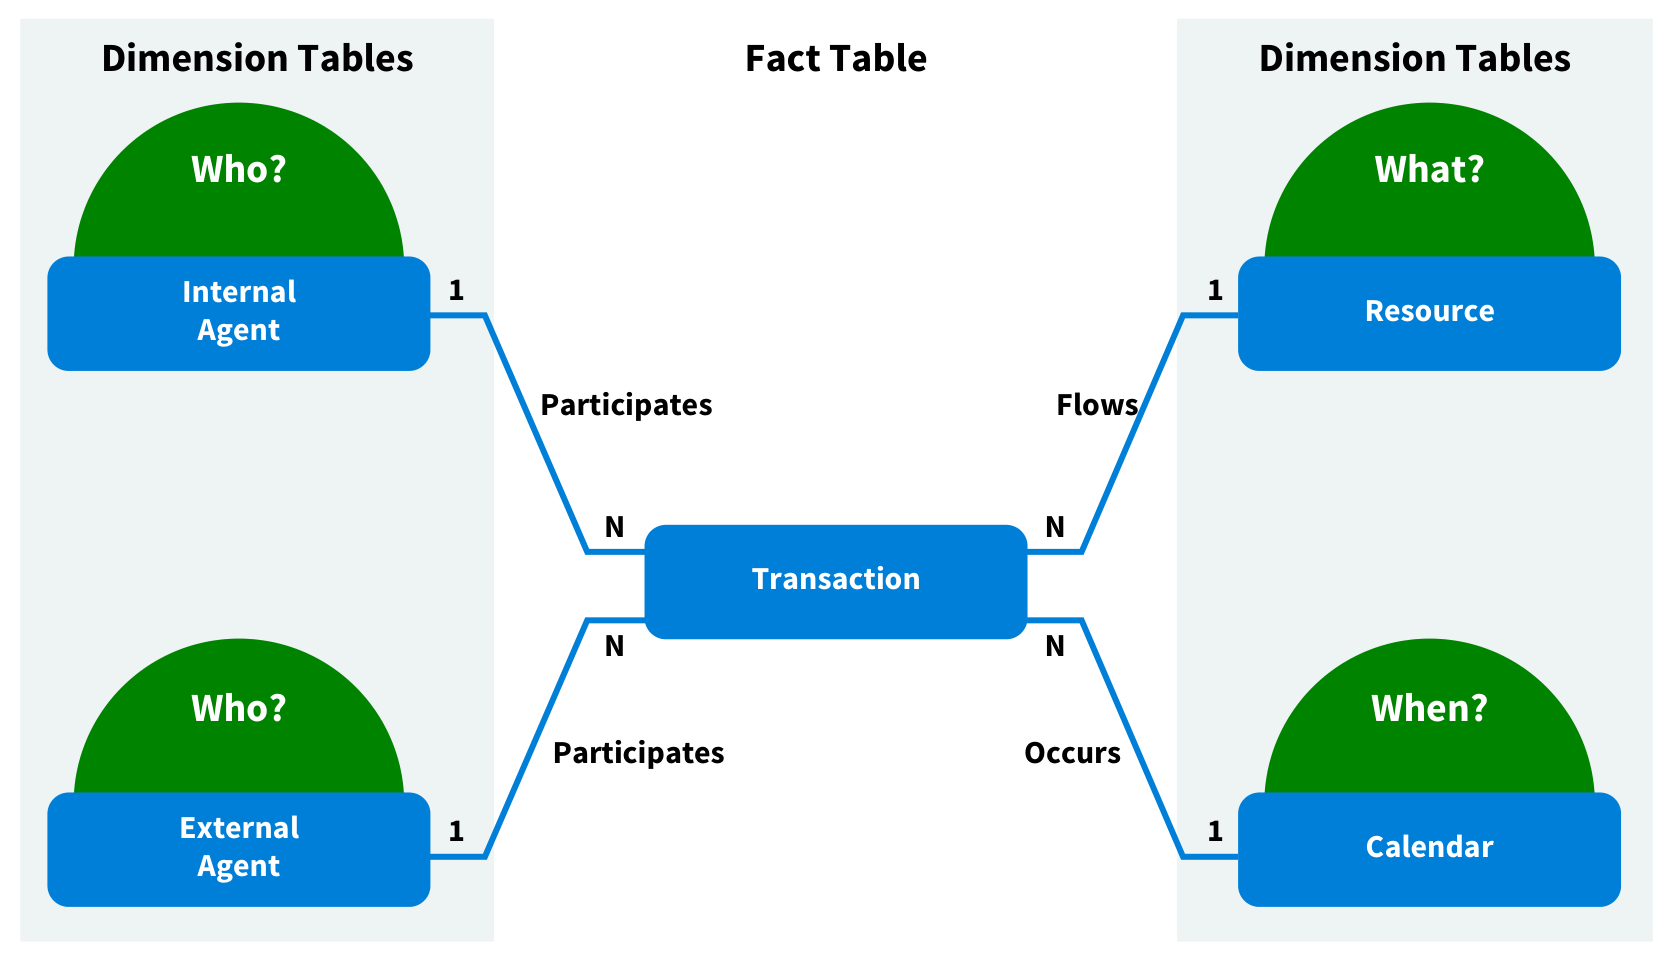
\includegraphics[width=0.95\textwidth,height=0.75\textheight,keepaspectratio]{../textbookForPractice/Figures/Ch_06/ILLUSTRATION 6.41.png}
    \end{figure}
\end{frame}

\begin{frame}{ILLUSTRATION 6.42}

    \begin{figure}[h]
        \centering
        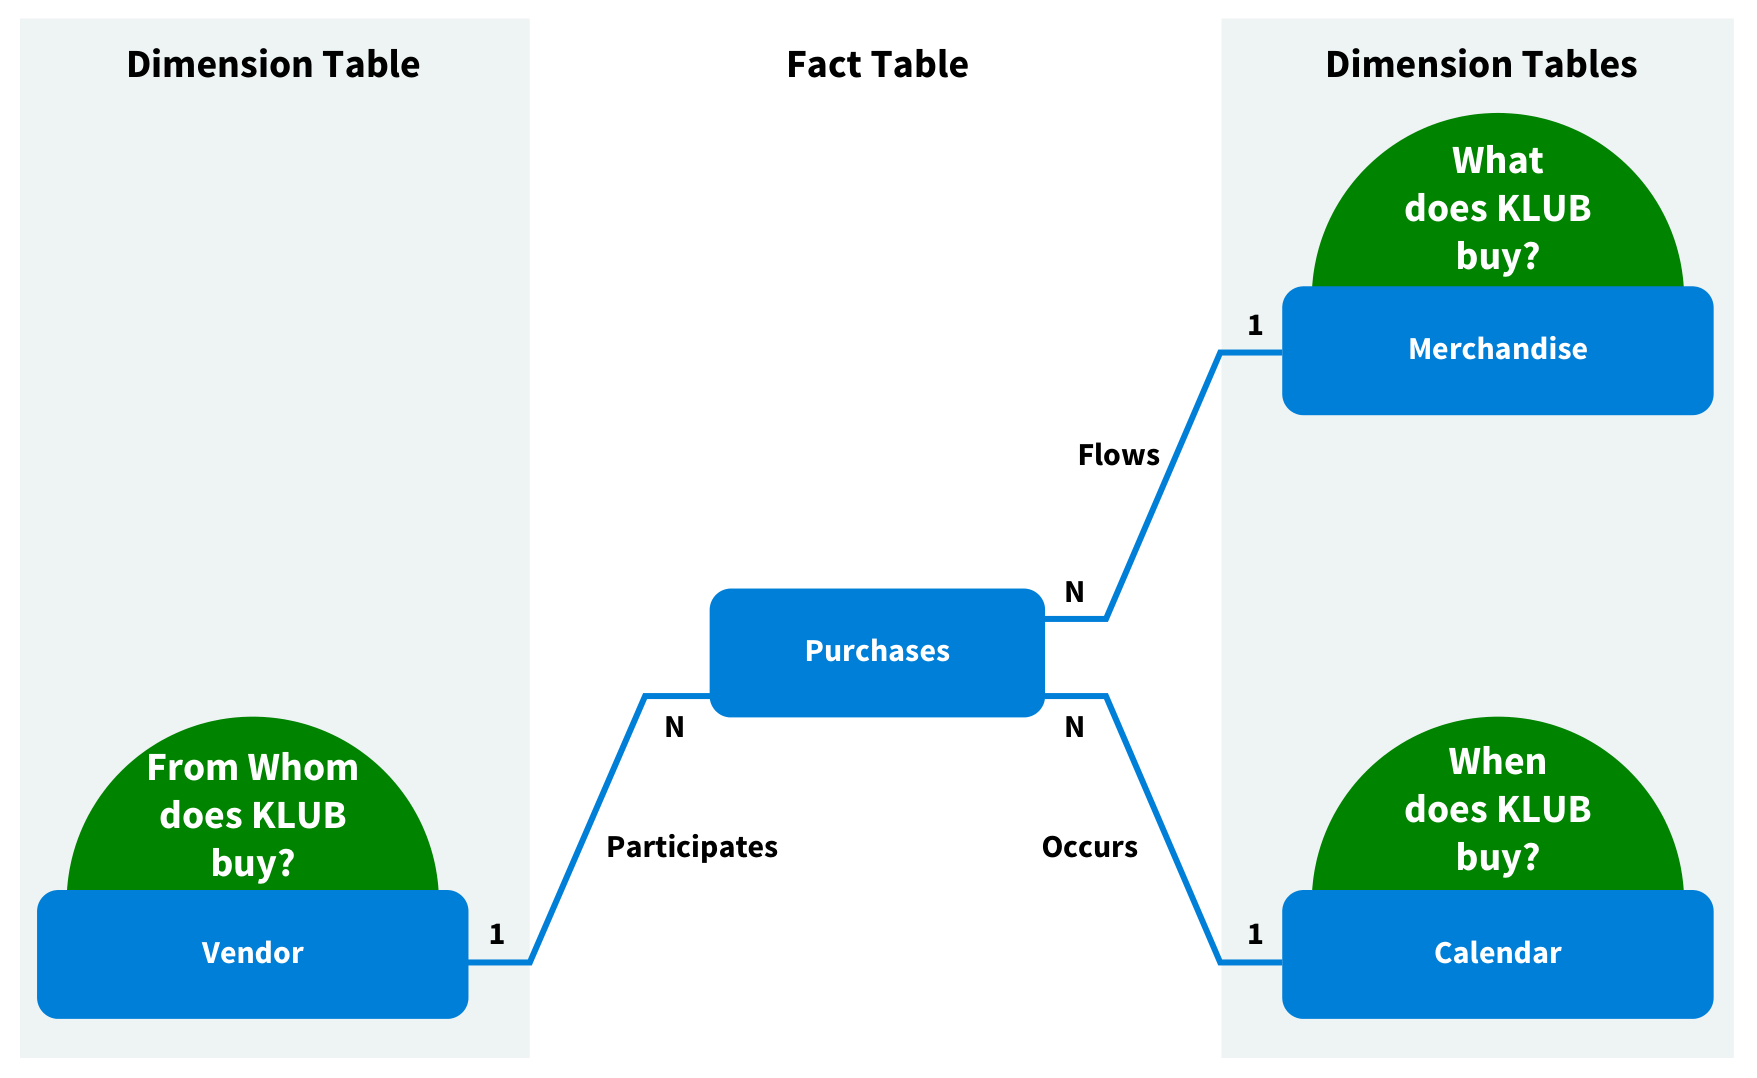
\includegraphics[width=0.95\textwidth,height=0.75\textheight,keepaspectratio]{../textbookForPractice/Figures/Ch_06/ILLUSTRATION 6.42.png}
    \end{figure}
\end{frame}

\begin{frame}{ILLUSTRATION 6.43}

    \begin{figure}[h]
        \centering
        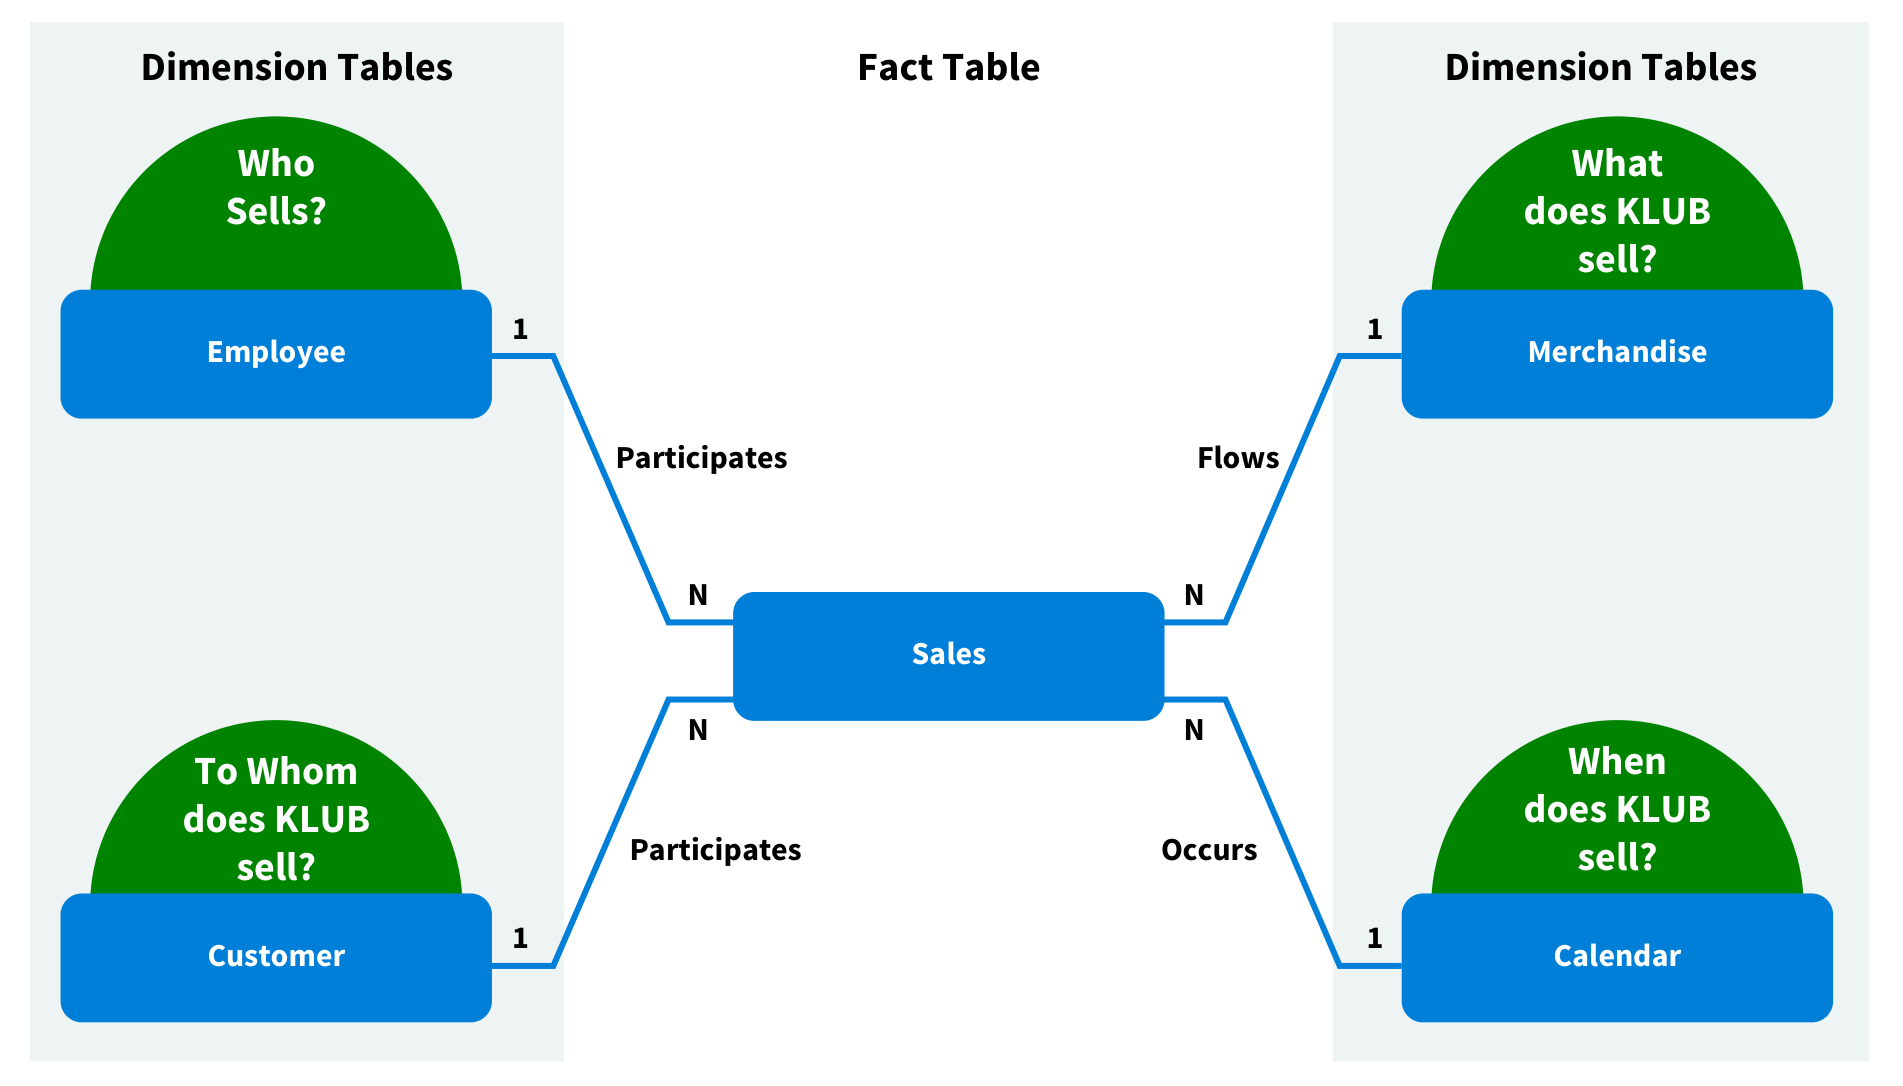
\includegraphics[width=0.95\textwidth,height=0.75\textheight,keepaspectratio]{../textbookForPractice/Figures/Ch_06/ILLUSTRATION 6.43.png}
    \end{figure}
\end{frame}

\begin{frame}{ILLUSTRATION 6.44}

    \begin{figure}[h]
        \centering
        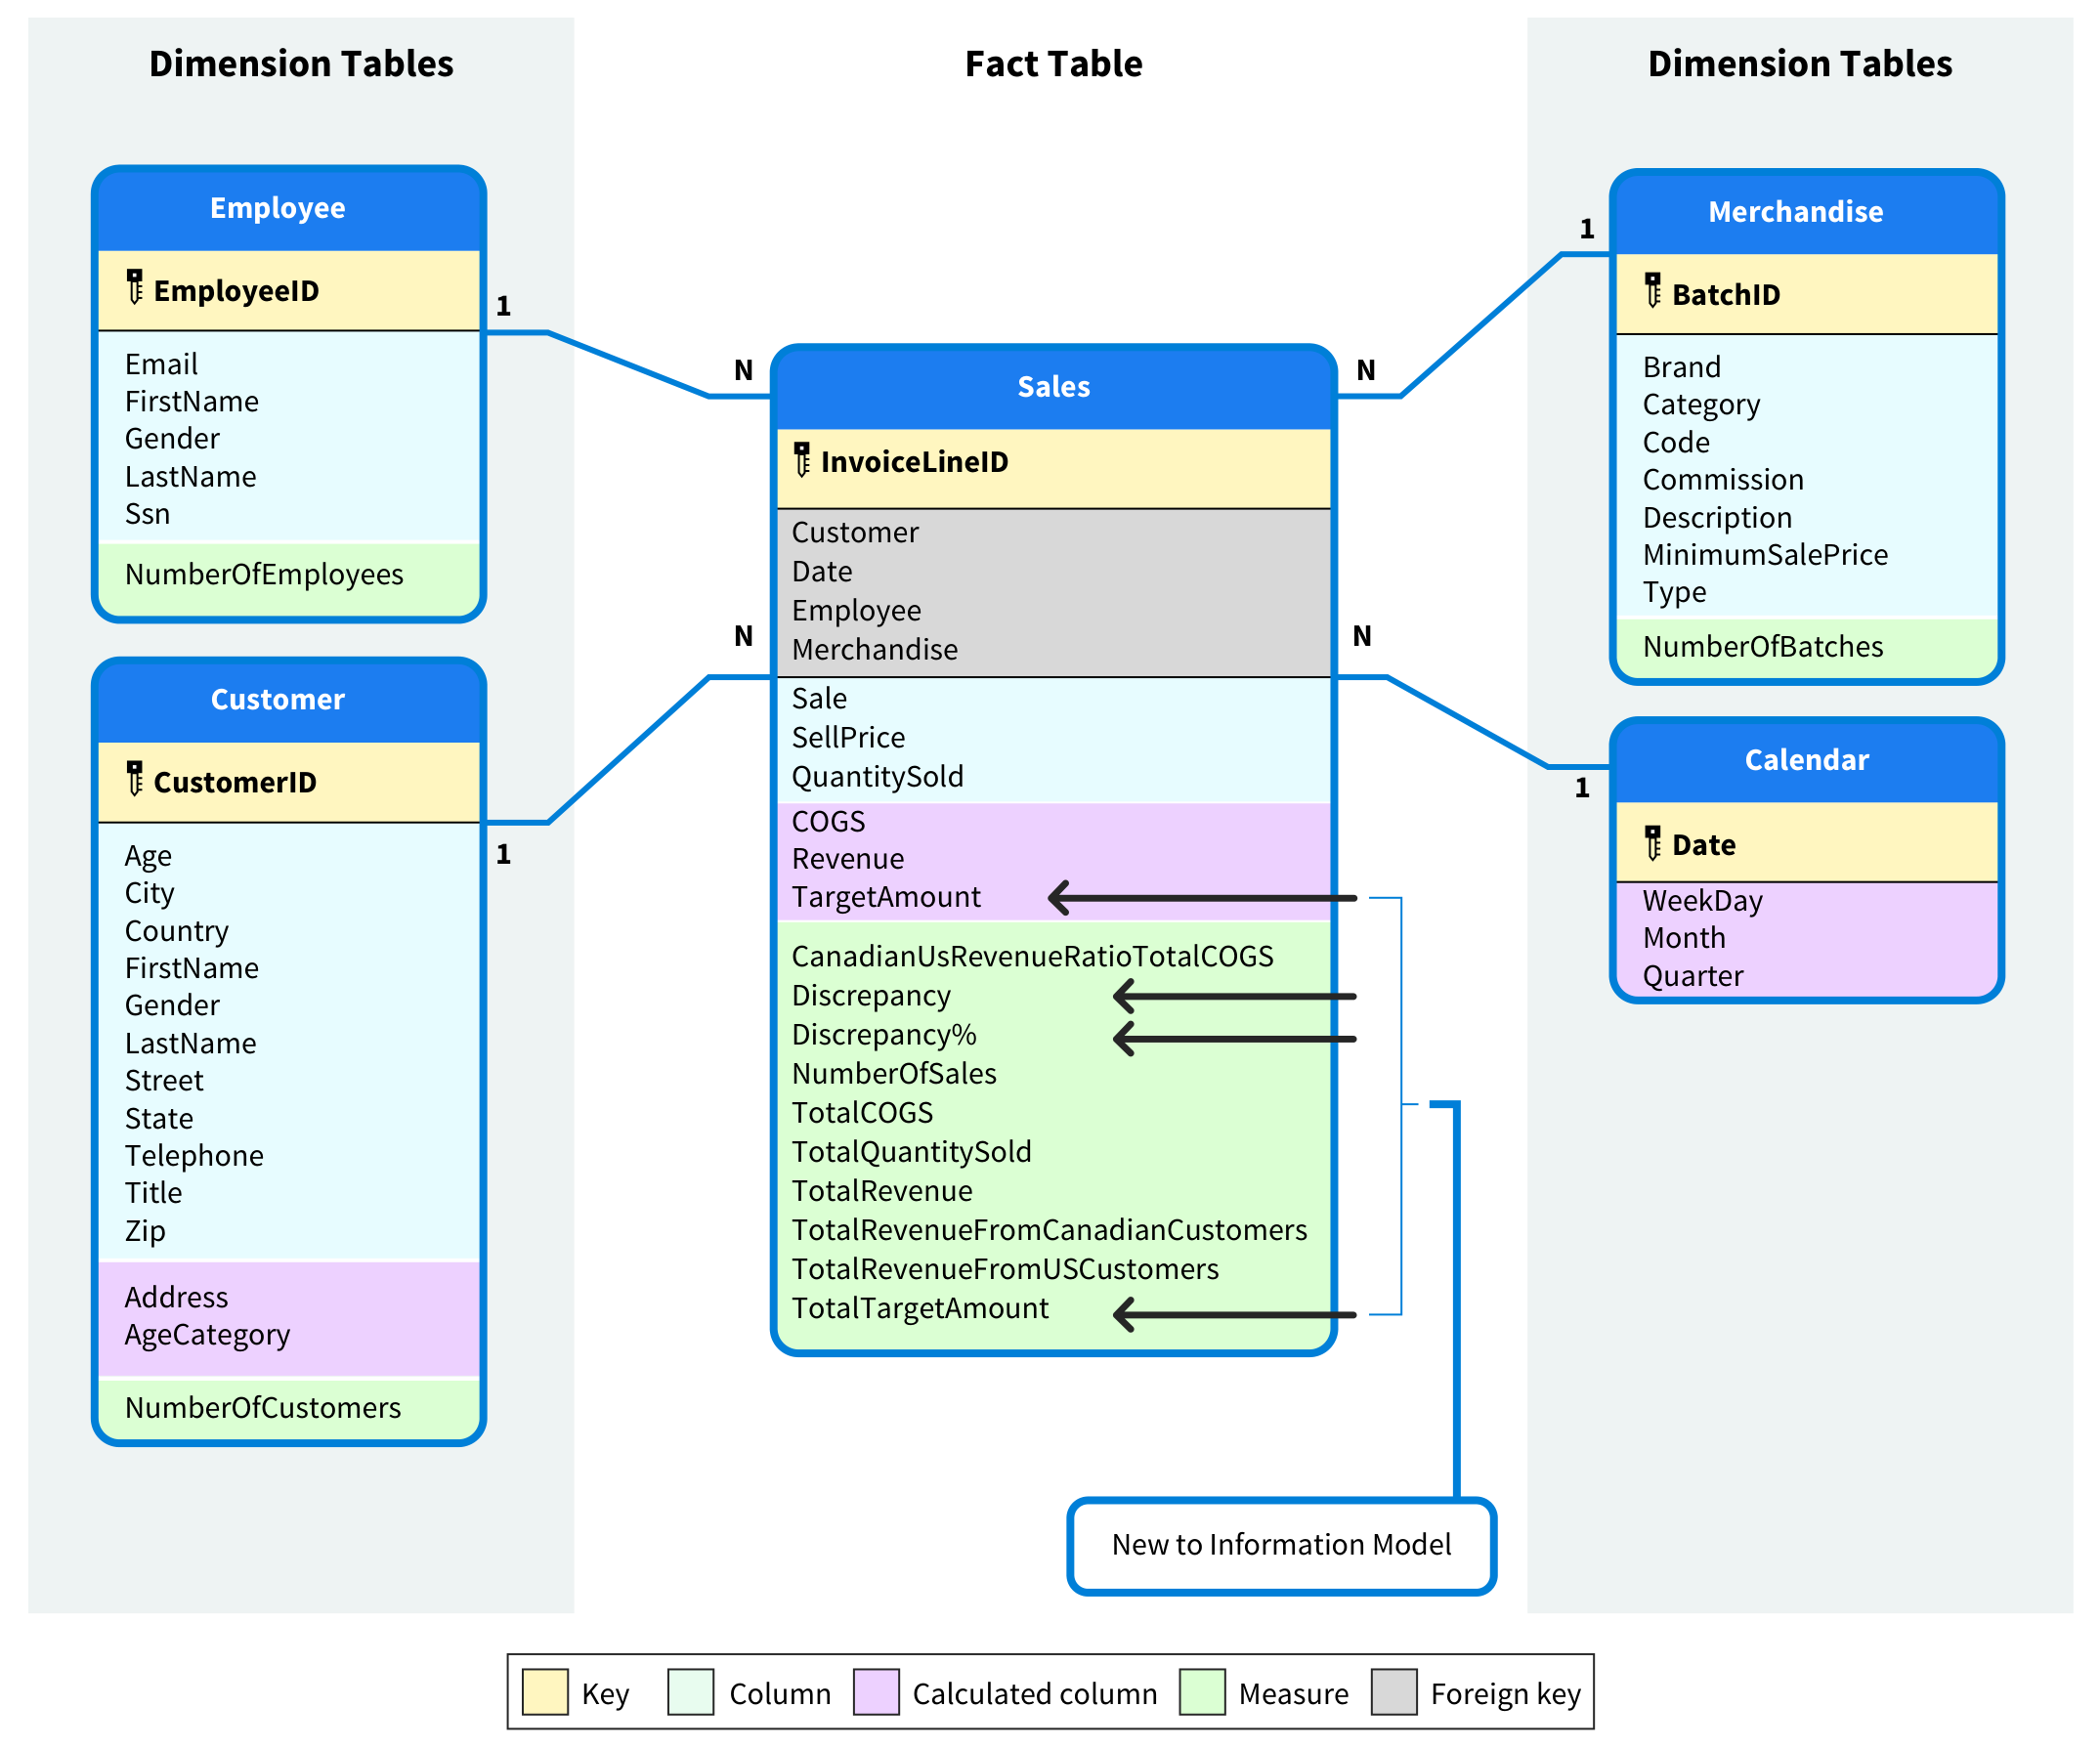
\includegraphics[width=0.95\textwidth,height=0.75\textheight,keepaspectratio]{../textbookForPractice/Figures/Ch_06/ILLUSTRATION 6.44.png}
    \end{figure}
\end{frame}

\begin{frame}{6.3 Sáu Mẫu Cấu trúc Dữ liệu Kế toán}
\begin{itemize}
    \item \textbf{Mẫu 1 - Hệ thống Tài khoản (Chart of Accounts):} Bảng danh mục cốt lõi của mọi hệ thống kế toán.
    \item \textbf{Mẫu 2 - Dữ liệu Giao dịch (Transactions):} Bảng Fact chứa các bút toán nhật ký (Sổ cái).
    \item \textbf{Mẫu 3 - Danh mục Thực thể (Entity/Master Data):} Khách hàng, Nhà cung cấp, Sản phẩm, Nhân viên.
\end{itemize}
\end{frame}

\begin{frame}{ILLUSTRATION 6.45}

    \begin{figure}[h]
        \centering
        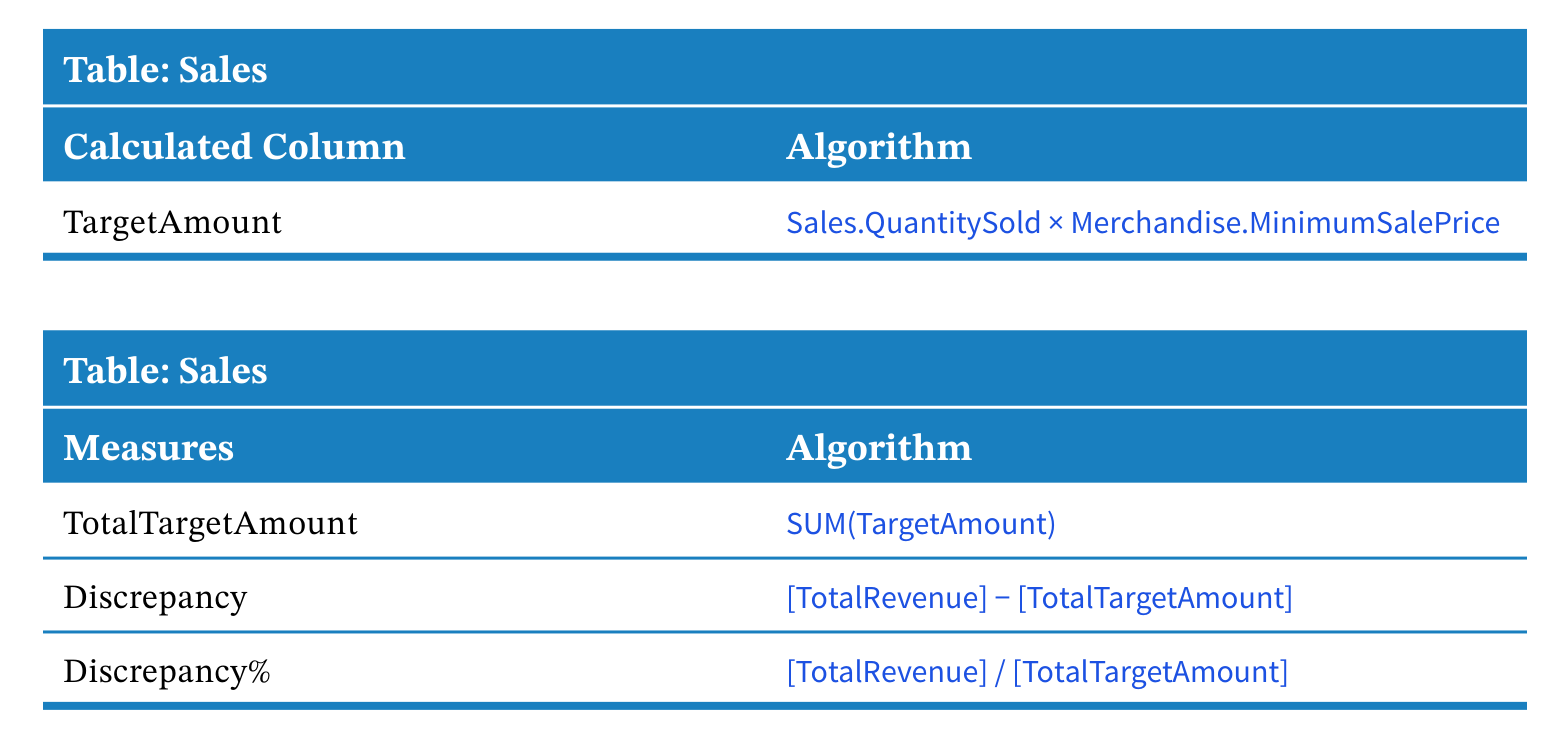
\includegraphics[width=0.95\textwidth,height=0.75\textheight,keepaspectratio]{../textbookForPractice/Figures/Ch_06/ILLUSTRATION 6.45.png}
    \end{figure}
\end{frame}

\begin{frame}{ILLUSTRATION 6.46}

    \begin{figure}[h]
        \centering
        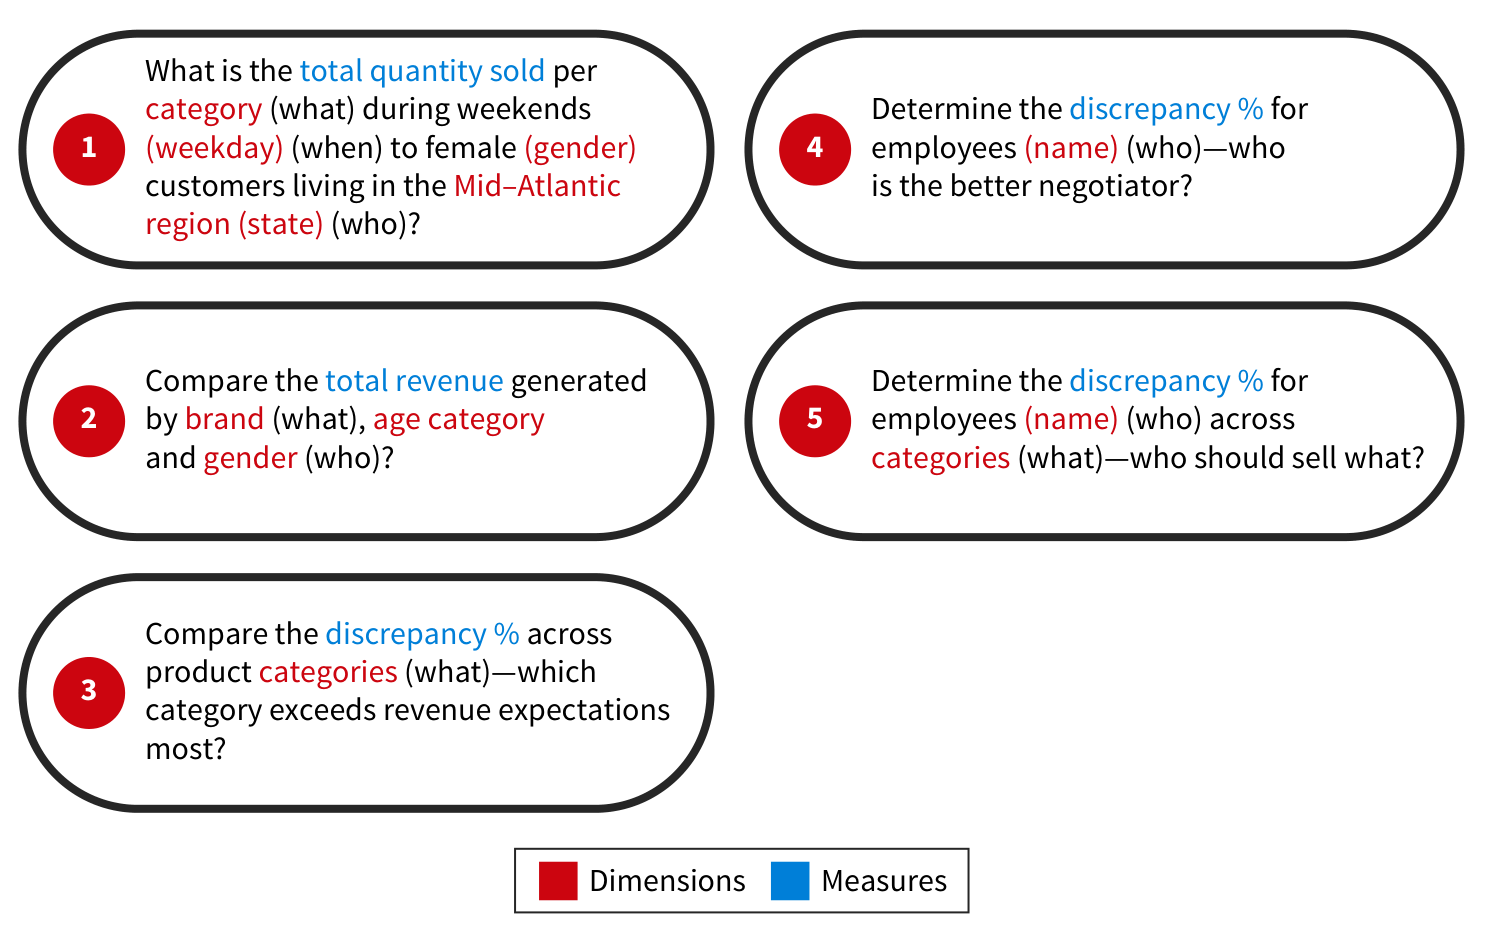
\includegraphics[width=0.95\textwidth,height=0.75\textheight,keepaspectratio]{../textbookForPractice/Figures/Ch_06/ILLUSTRATION 6.46.png}
    \end{figure}
\end{frame}

\begin{frame}{ILLUSTRATION 6.47}

    \begin{figure}[h]
        \centering
        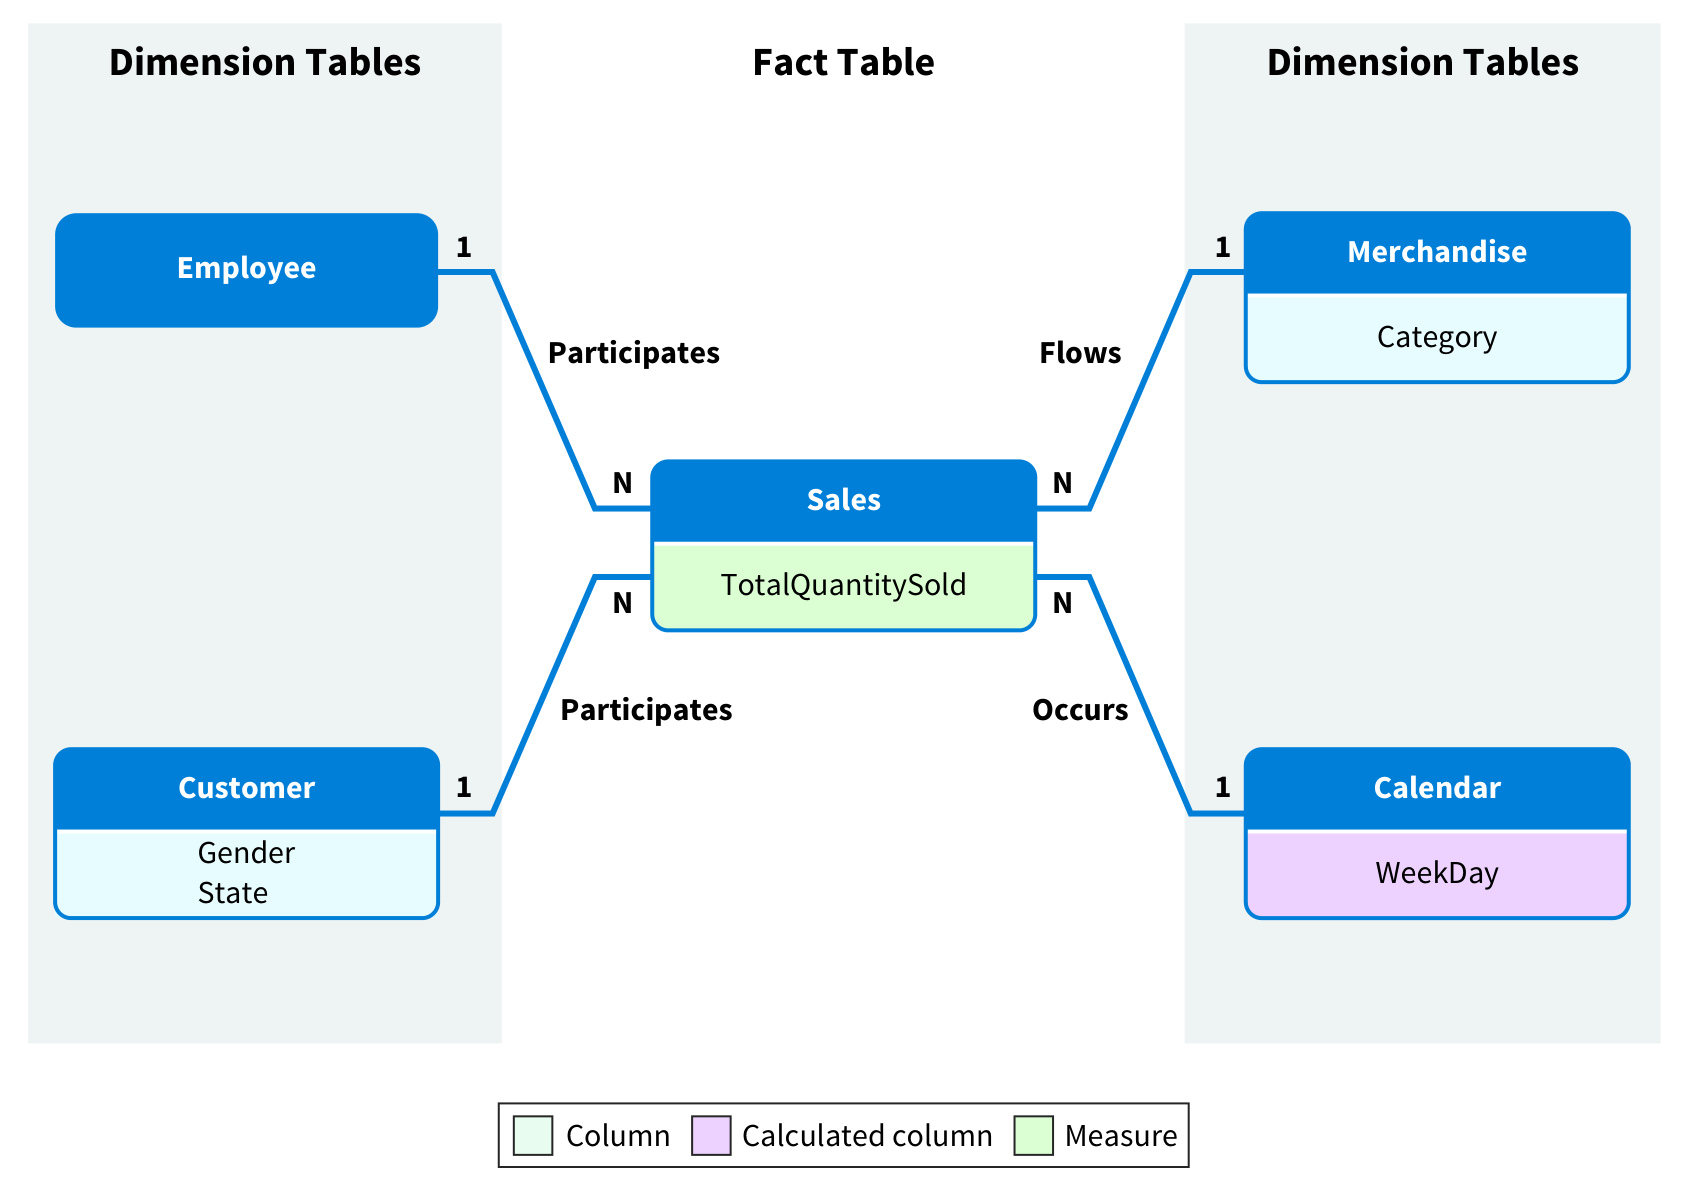
\includegraphics[width=0.95\textwidth,height=0.75\textheight,keepaspectratio]{../textbookForPractice/Figures/Ch_06/ILLUSTRATION 6.47.png}
    \end{figure}
\end{frame}

\begin{frame}{ILLUSTRATION 6.48}

    \begin{figure}[h]
        \centering
        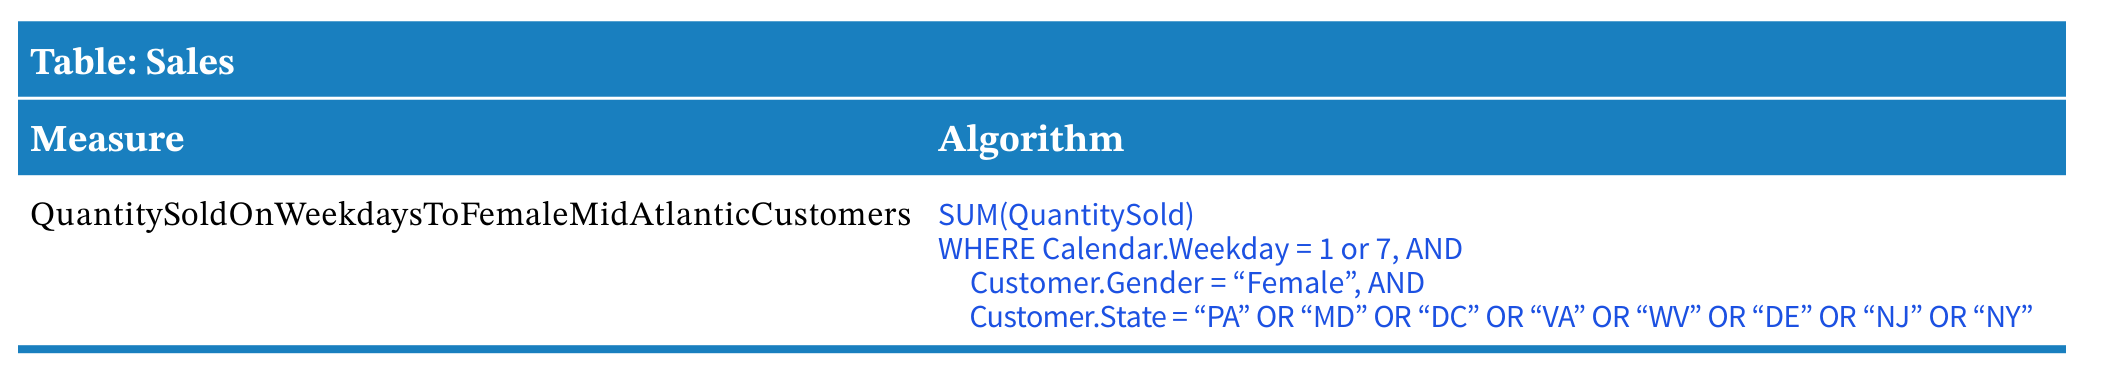
\includegraphics[width=0.95\textwidth,height=0.75\textheight,keepaspectratio]{../textbookForPractice/Figures/Ch_06/ILLUSTRATION 6.48.png}
    \end{figure}
\end{frame}

\begin{frame}{ILLUSTRATION 6.49}

    \begin{figure}[h]
        \centering
        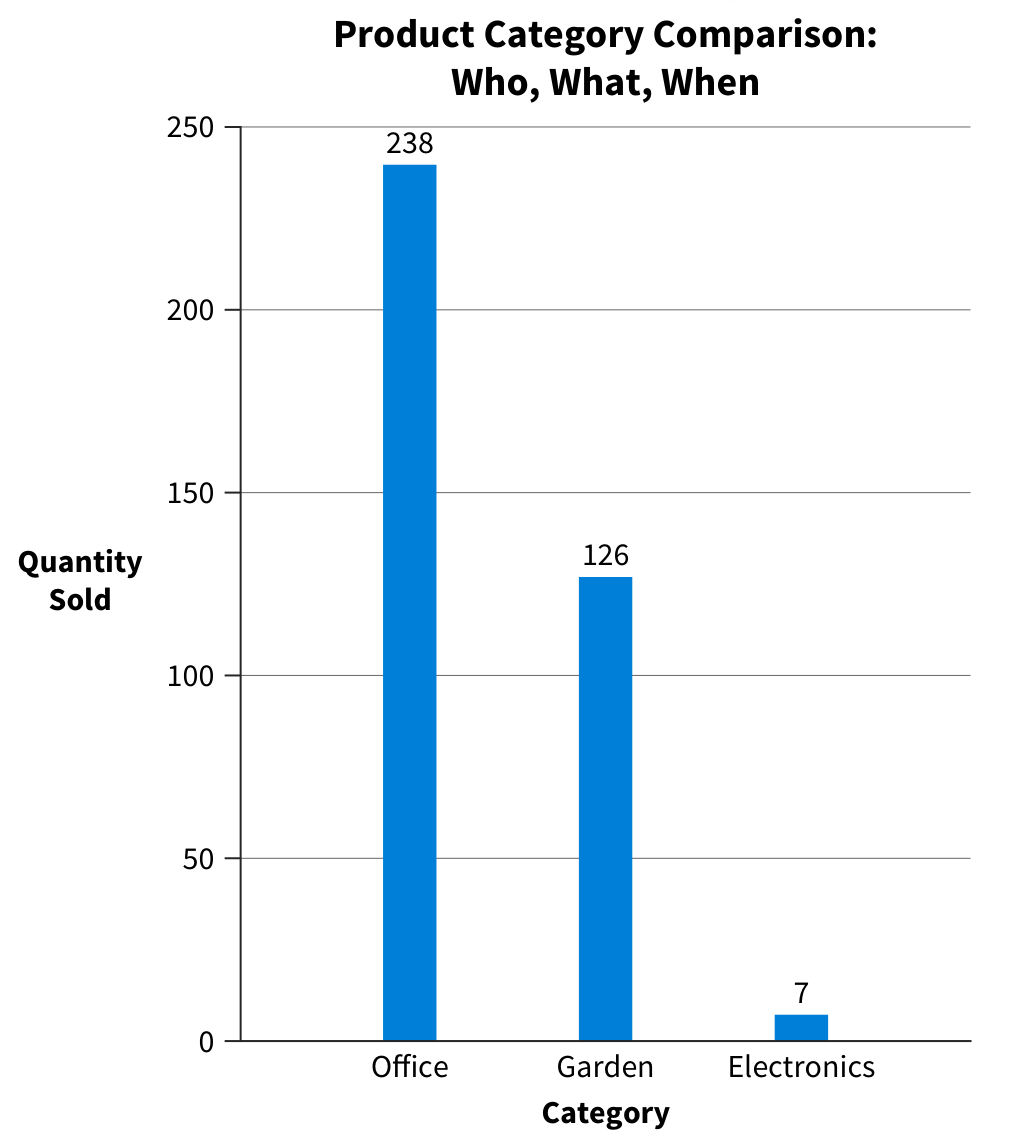
\includegraphics[width=0.95\textwidth,height=0.75\textheight,keepaspectratio]{../textbookForPractice/Figures/Ch_06/ILLUSTRATION 6.49.png}
    \end{figure}
\end{frame}

\begin{frame}{ILLUSTRATION 6.50}

    \begin{figure}[h]
        \centering
        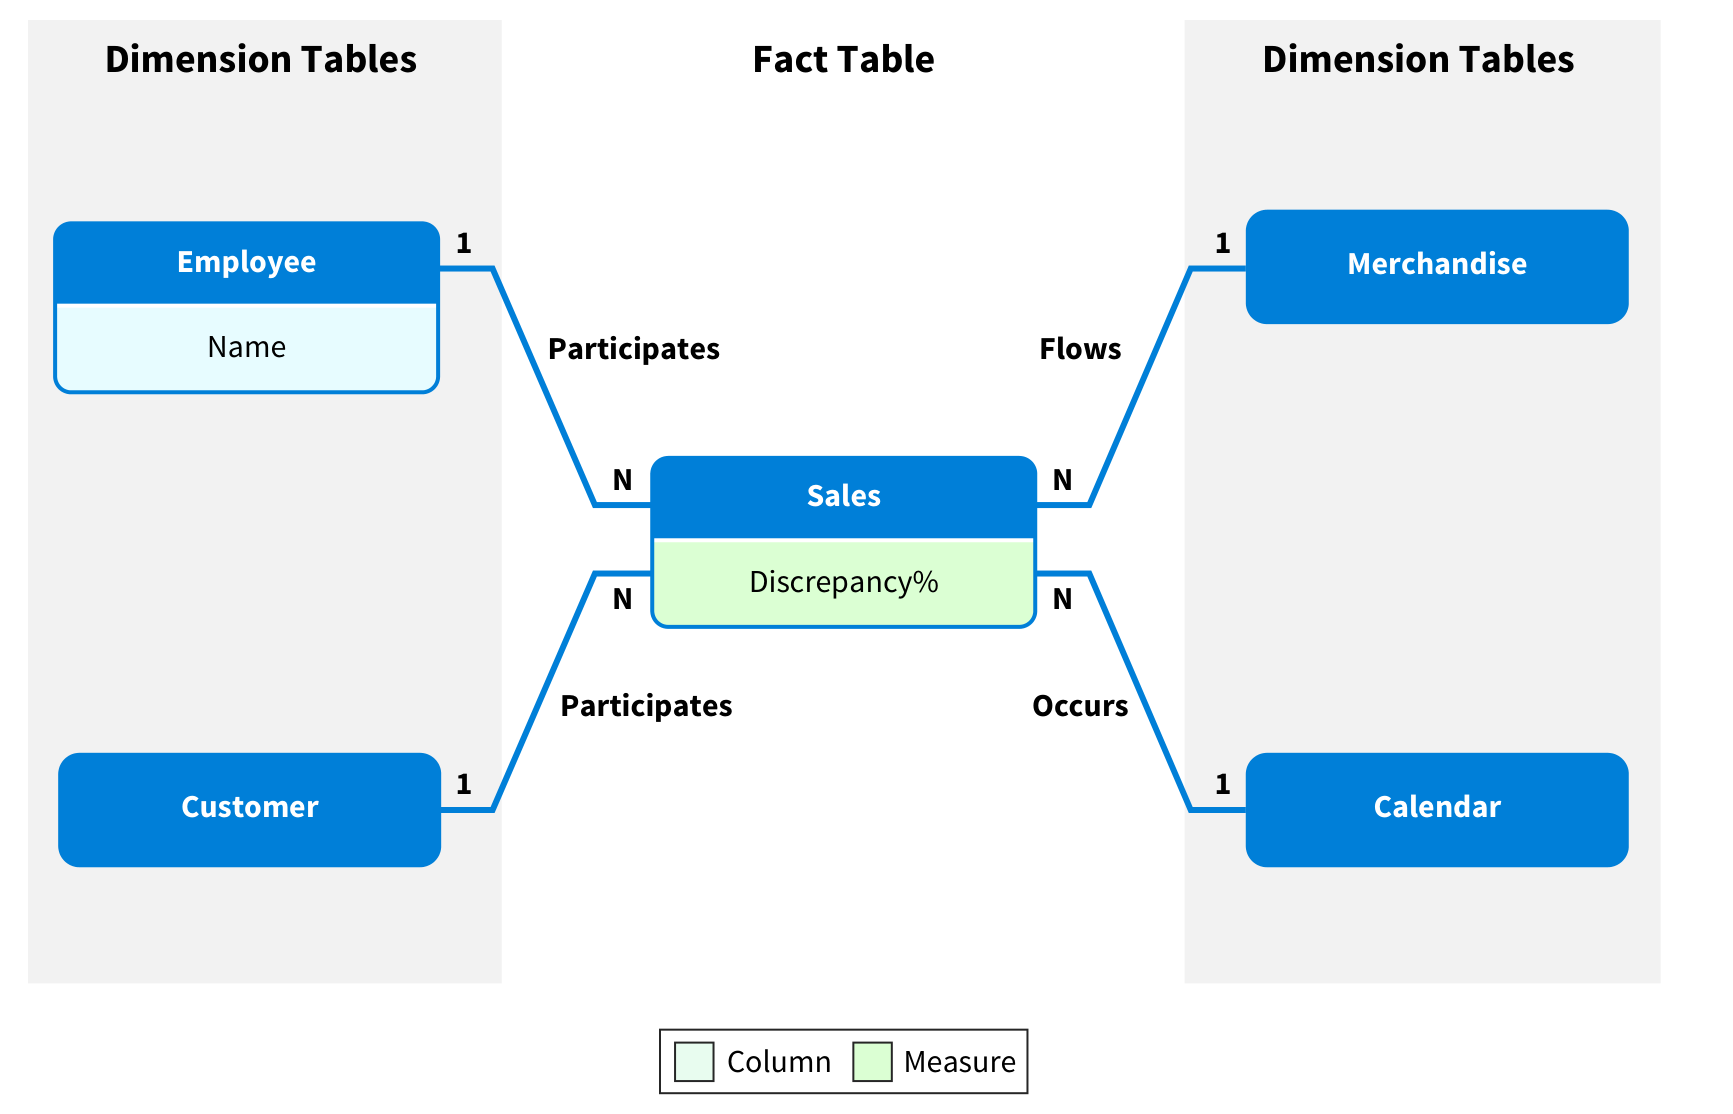
\includegraphics[width=0.95\textwidth,height=0.75\textheight,keepaspectratio]{../textbookForPractice/Figures/Ch_06/ILLUSTRATION 6.50.png}
    \end{figure}
\end{frame}

\begin{frame}{ILLUSTRATION 6.51}

    \begin{figure}[h]
        \centering
        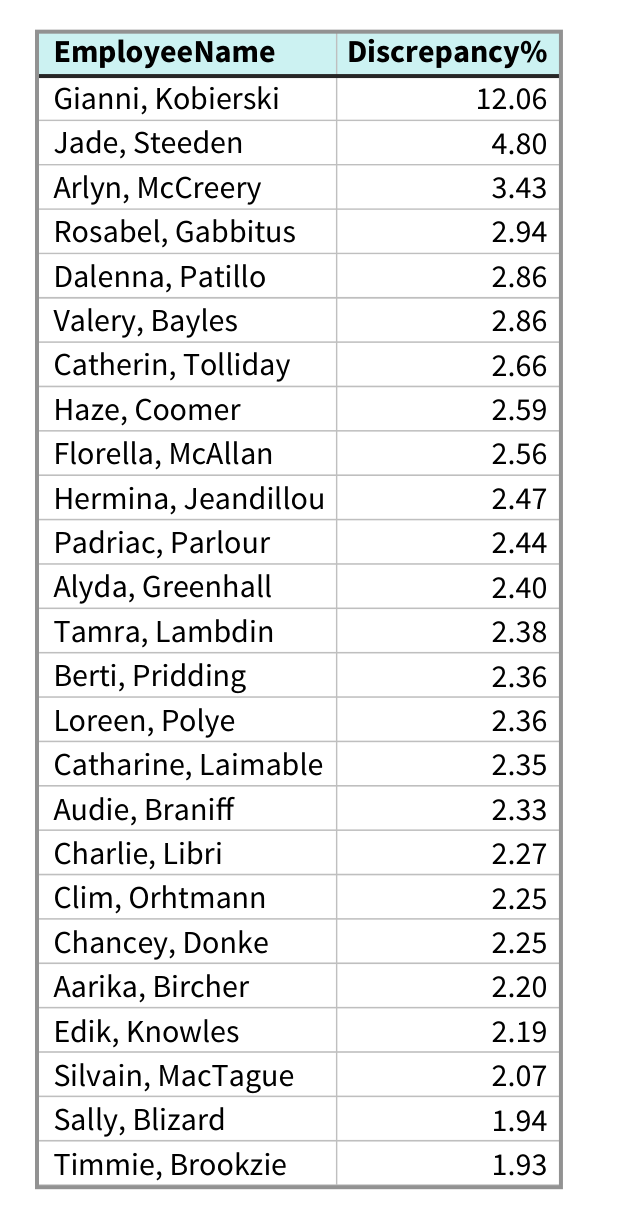
\includegraphics[width=0.95\textwidth,height=0.75\textheight,keepaspectratio]{../textbookForPractice/Figures/Ch_06/ILLUSTRATION 6.51.png}
    \end{figure}
\end{frame}

\begin{frame}{ILLUSTRATION 6.52}

    \begin{figure}[h]
        \centering
        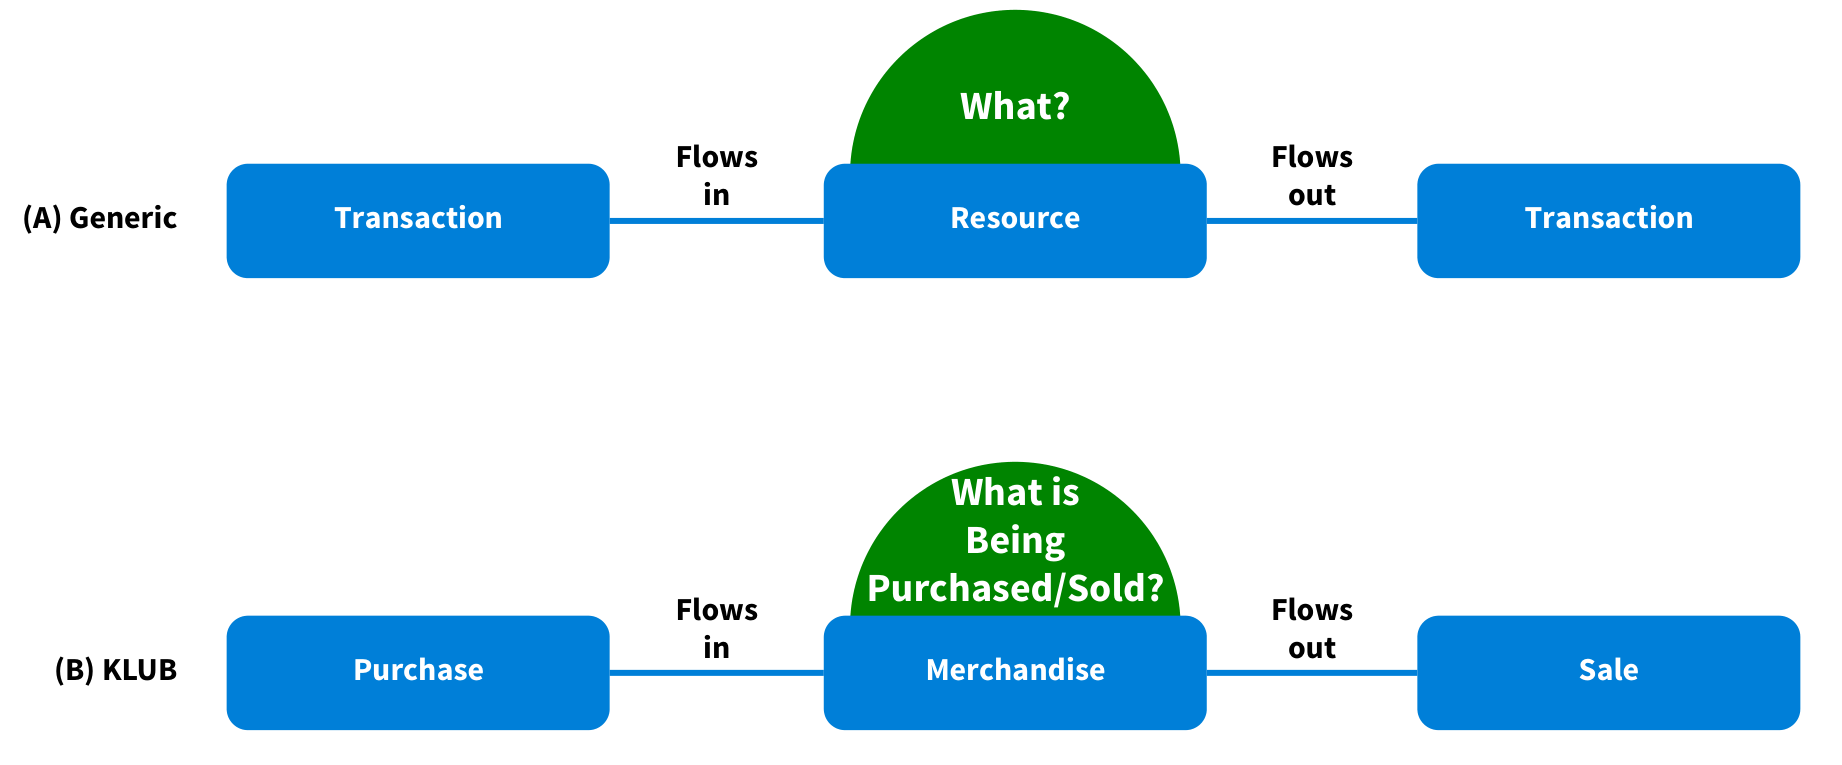
\includegraphics[width=0.95\textwidth,height=0.75\textheight,keepaspectratio]{../textbookForPractice/Figures/Ch_06/ILLUSTRATION 6.52.png}
    \end{figure}
\end{frame}

\begin{frame}{ILLUSTRATION 6.53}

    \begin{figure}[h]
        \centering
        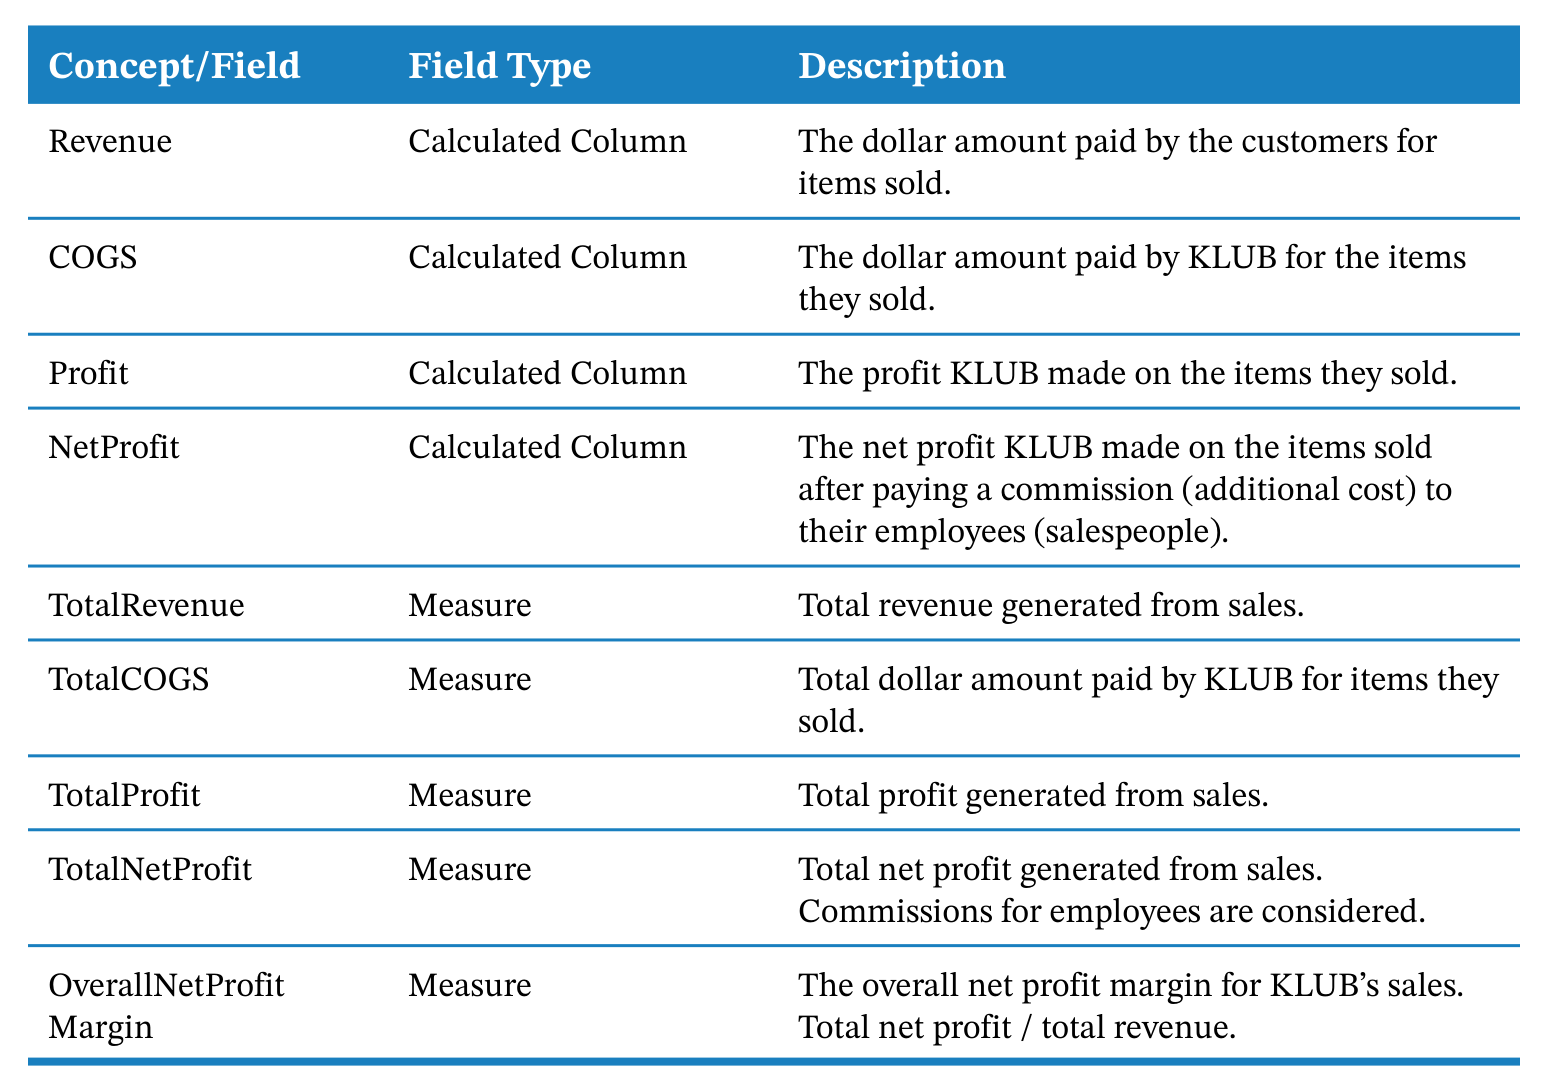
\includegraphics[width=0.95\textwidth,height=0.75\textheight,keepaspectratio]{../textbookForPractice/Figures/Ch_06/ILLUSTRATION 6.53.png}
    \end{figure}
\end{frame}

\begin{frame}{ILLUSTRATION 6.54}

    \begin{figure}[h]
        \centering
        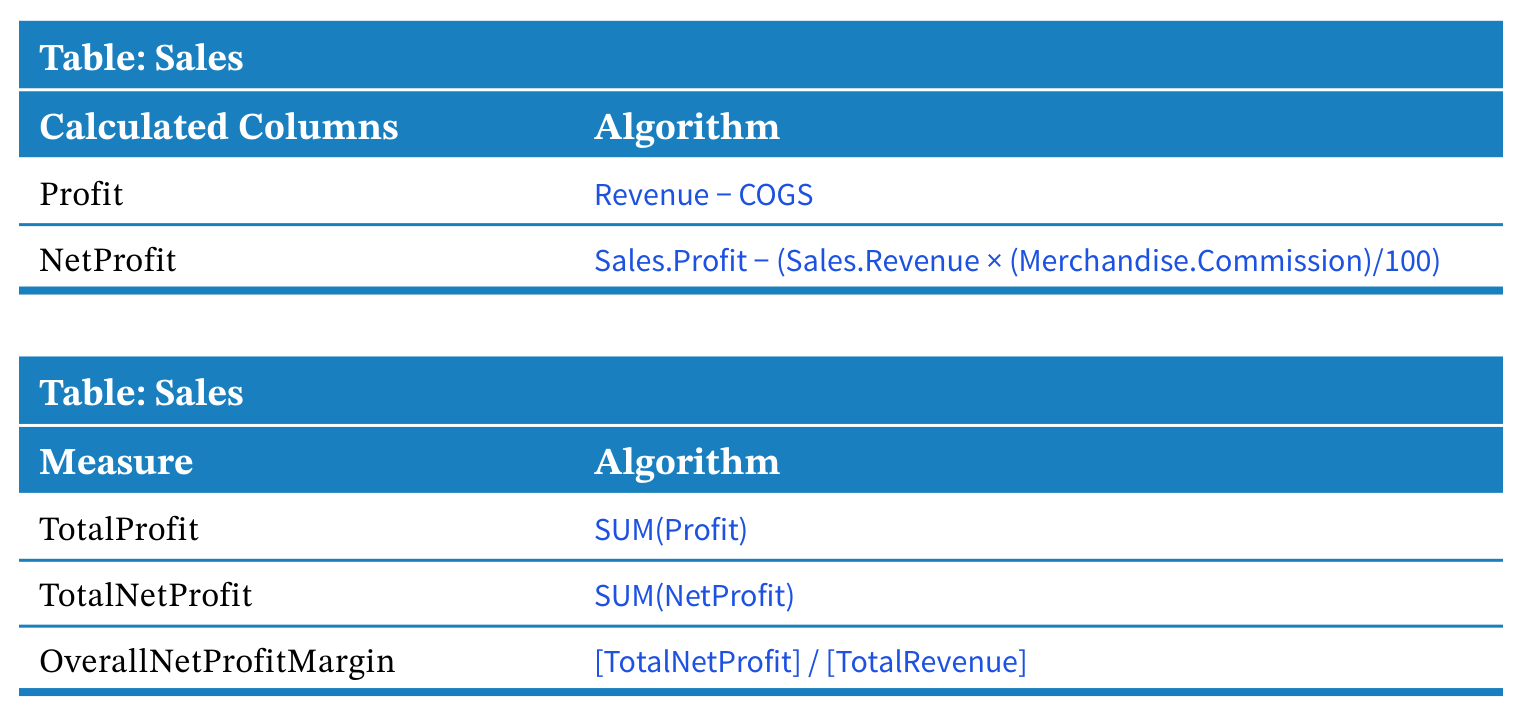
\includegraphics[width=0.95\textwidth,height=0.75\textheight,keepaspectratio]{../textbookForPractice/Figures/Ch_06/ILLUSTRATION 6.54.png}
    \end{figure}
\end{frame}

\begin{frame}{ILLUSTRATION 6.55}

    \begin{figure}[h]
        \centering
        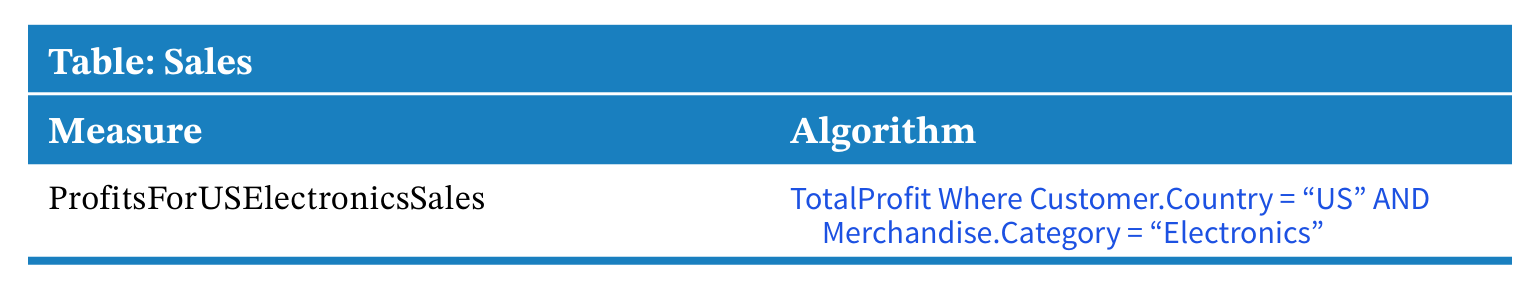
\includegraphics[width=0.95\textwidth,height=0.75\textheight,keepaspectratio]{../textbookForPractice/Figures/Ch_06/ILLUSTRATION 6.55.png}
    \end{figure}
\end{frame}

\begin{frame}{Cấu trúc Dữ liệu (Tiếp theo)}
\begin{itemize}
    \item \textbf{Mẫu 4 - Ngân sách so với Thực tế (Budget vs Actual):} Kết nối bảng kế hoạch và bảng thực tế để phân tích chênh lệch (Variance Analysis).
    \item \textbf{Mẫu 5 - Bảng Thời gian (Time Dimension):} Cực kỳ quan trọng để phân tích xu hướng (Time Intelligence) trong Power BI / Tableau.
    \item \textbf{Mẫu 6 - Sổ cái và Sổ chi tiết (General \& Subsidiary Ledgers):} Mối quan hệ 1-N (One-to-Many) giữa Sổ cái tổng hợp và các Sổ chi tiết (Phải thu, Phải trả, Hàng tồn kho).
\end{itemize}
\end{frame}

\begin{frame}{ILLUSTRATION 6.56}

    \begin{figure}[h]
        \centering
        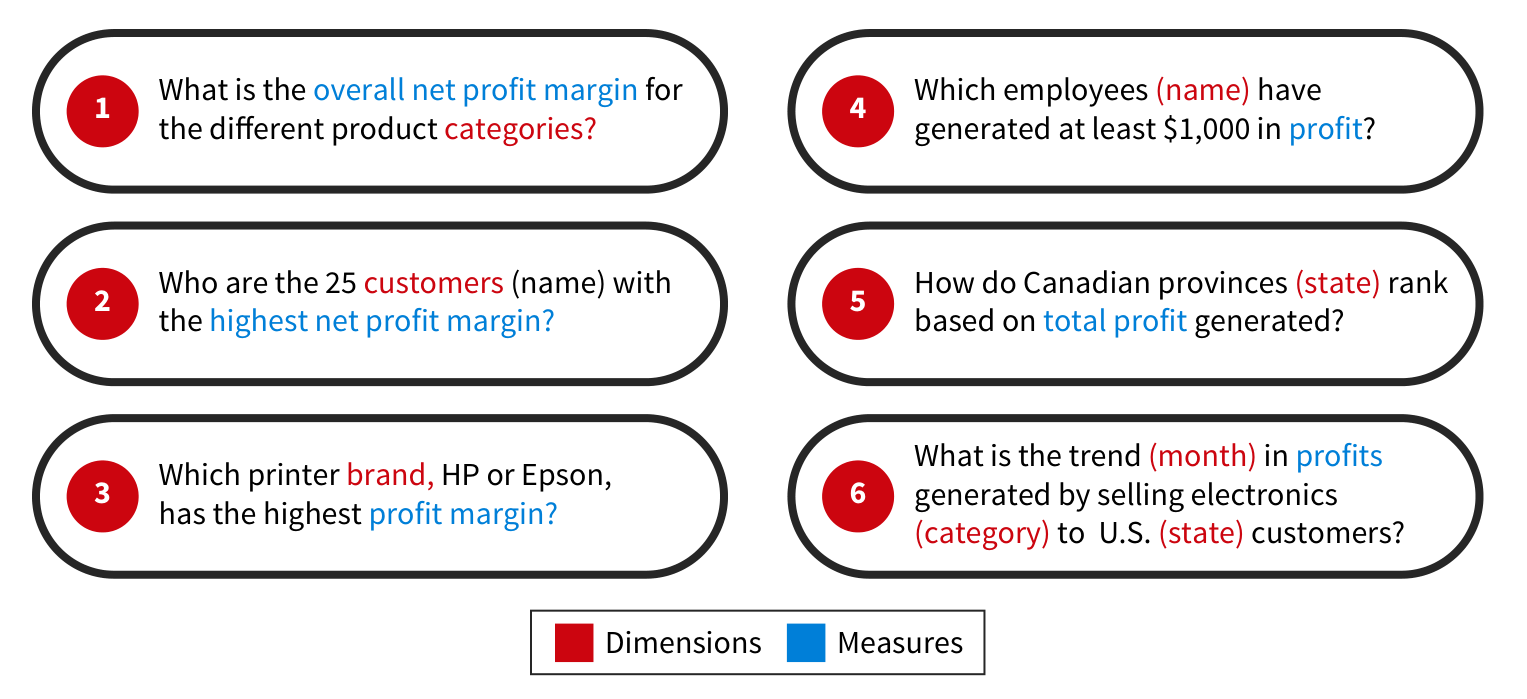
\includegraphics[width=0.95\textwidth,height=0.75\textheight,keepaspectratio]{../textbookForPractice/Figures/Ch_06/ILLUSTRATION 6.56.png}
    \end{figure}
\end{frame}

\begin{frame}{ILLUSTRATION 6.57}

    \begin{figure}[h]
        \centering
        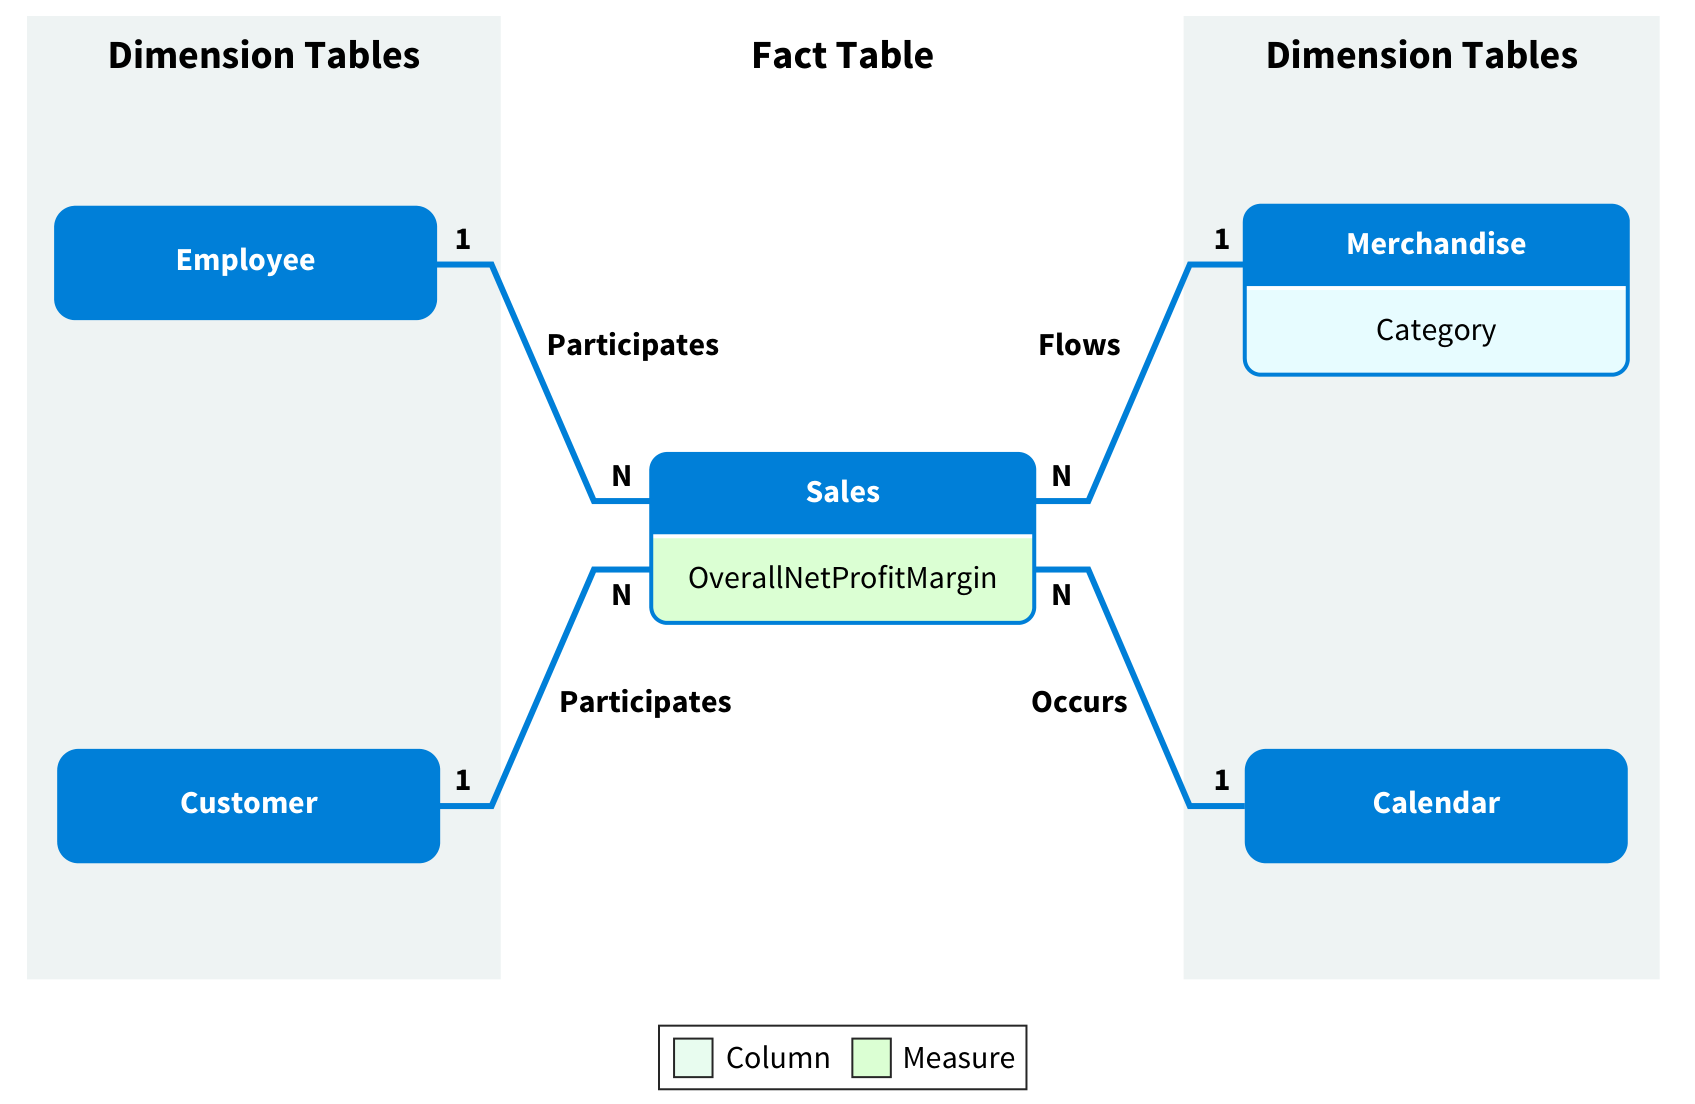
\includegraphics[width=0.95\textwidth,height=0.75\textheight,keepaspectratio]{../textbookForPractice/Figures/Ch_06/ILLUSTRATION 6.57.png}
    \end{figure}
\end{frame}

\begin{frame}{ILLUSTRATION 6.58}

    \begin{figure}[h]
        \centering
        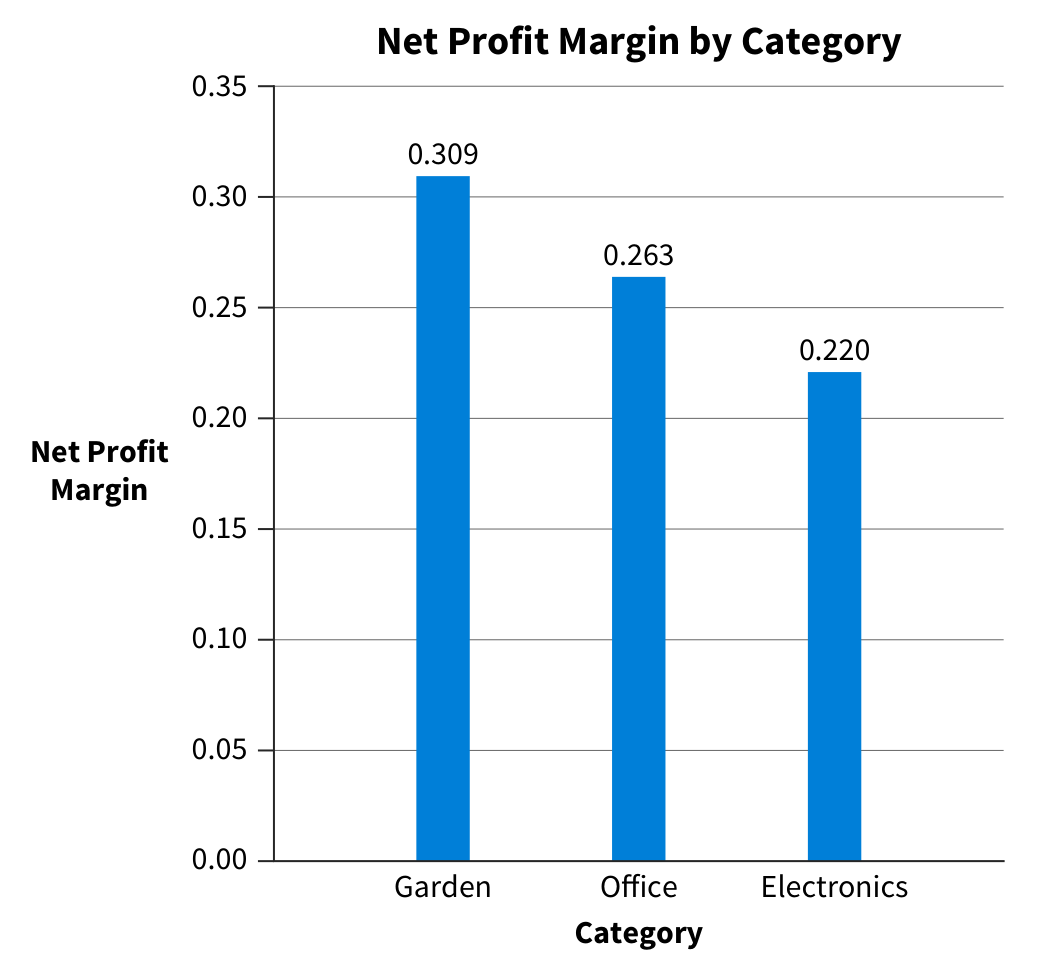
\includegraphics[width=0.95\textwidth,height=0.75\textheight,keepaspectratio]{../textbookForPractice/Figures/Ch_06/ILLUSTRATION 6.58.png}
    \end{figure}
\end{frame}

\begin{frame}{ILLUSTRATION 6.59}

    \begin{figure}[h]
        \centering
        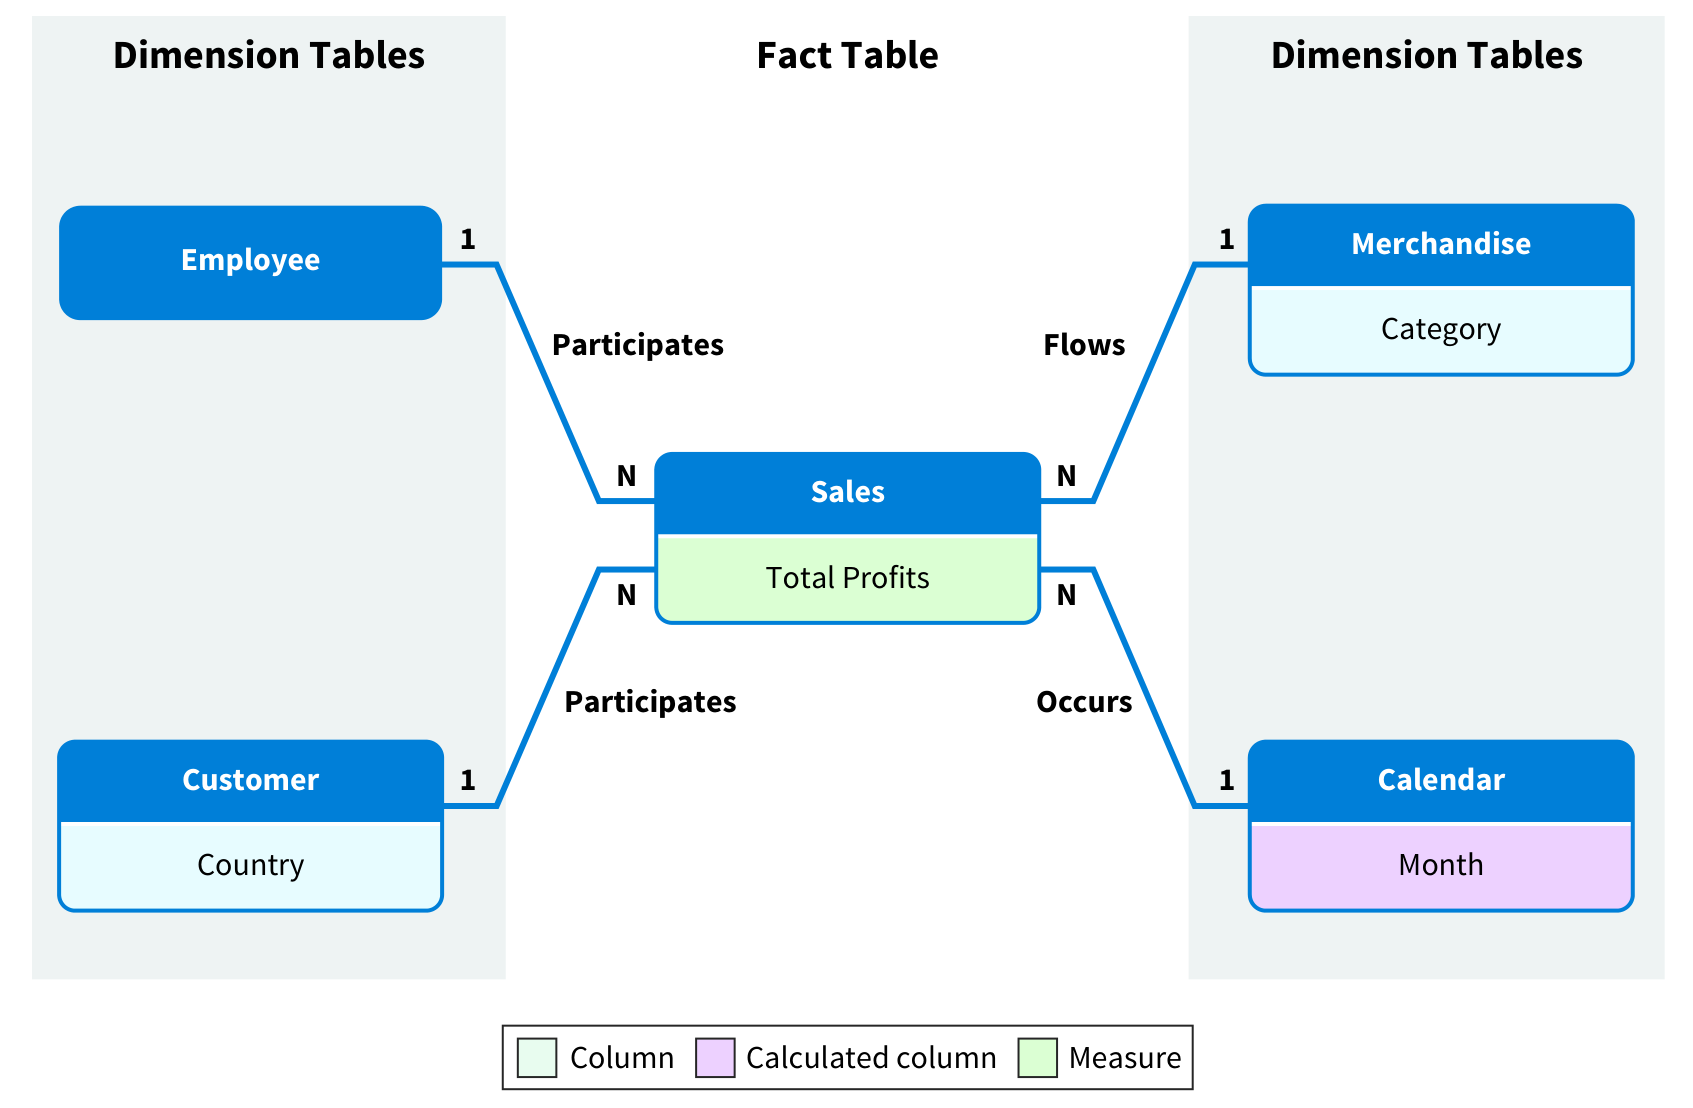
\includegraphics[width=0.95\textwidth,height=0.75\textheight,keepaspectratio]{../textbookForPractice/Figures/Ch_06/ILLUSTRATION 6.59.png}
    \end{figure}
\end{frame}

\begin{frame}{ILLUSTRATION 6.60}

    \begin{figure}[h]
        \centering
        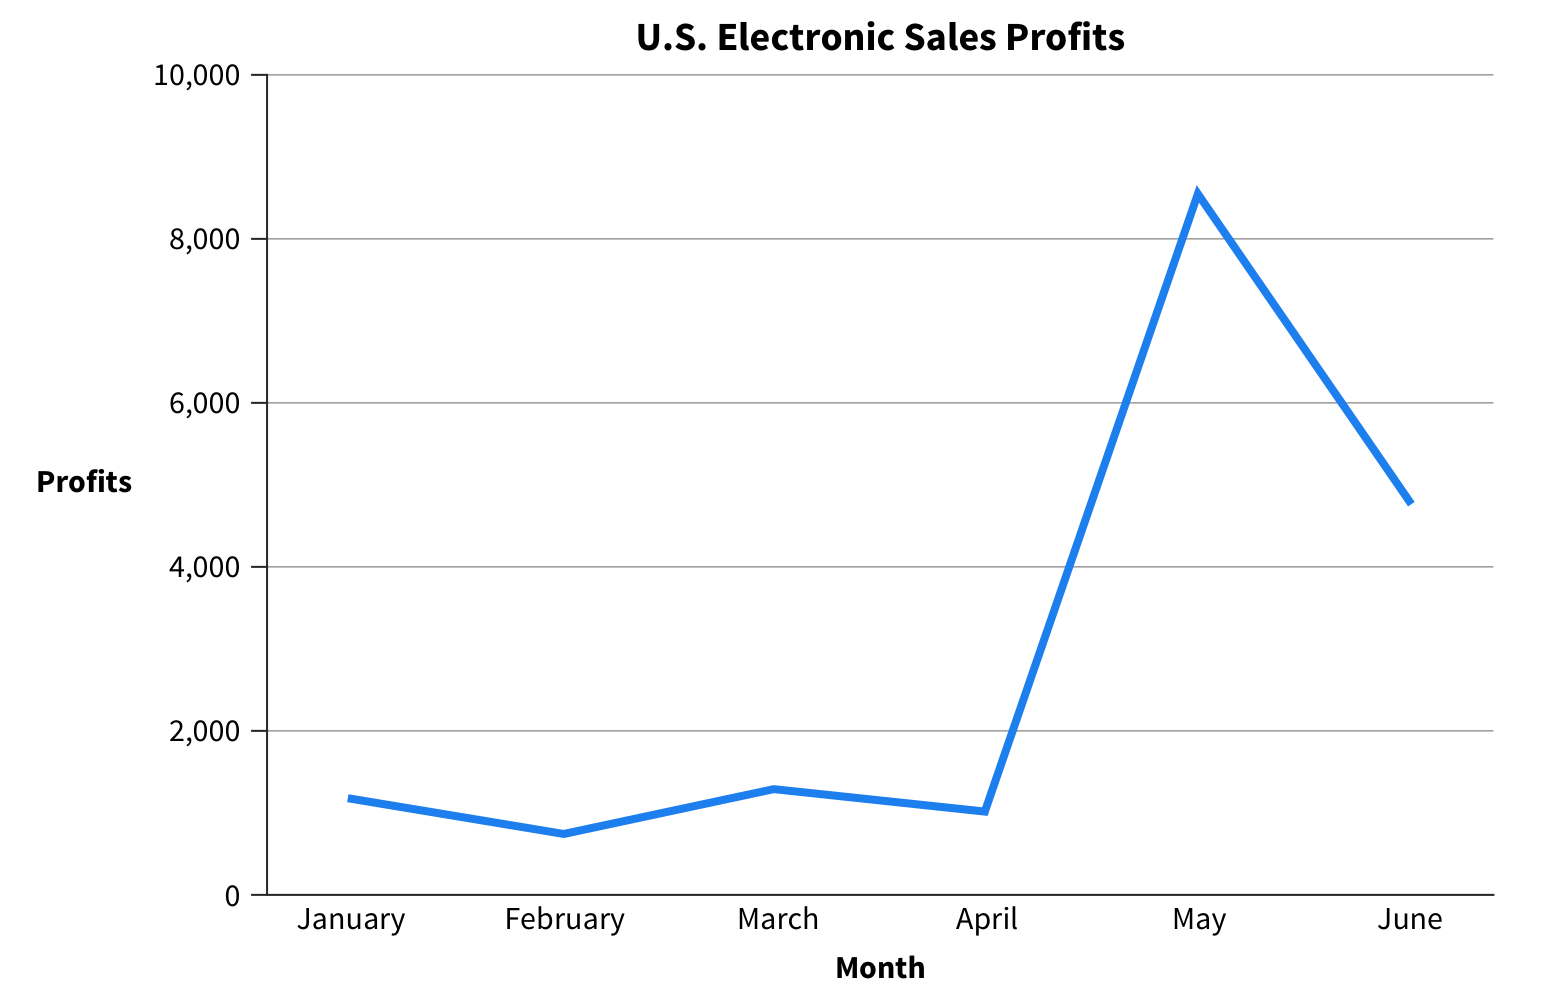
\includegraphics[width=0.95\textwidth,height=0.75\textheight,keepaspectratio]{../textbookForPractice/Figures/Ch_06/ILLUSTRATION 6.60.png}
    \end{figure}
\end{frame}

\begin{frame}{ILLUSTRATION 6.61A}

    \begin{figure}[h]
        \centering
        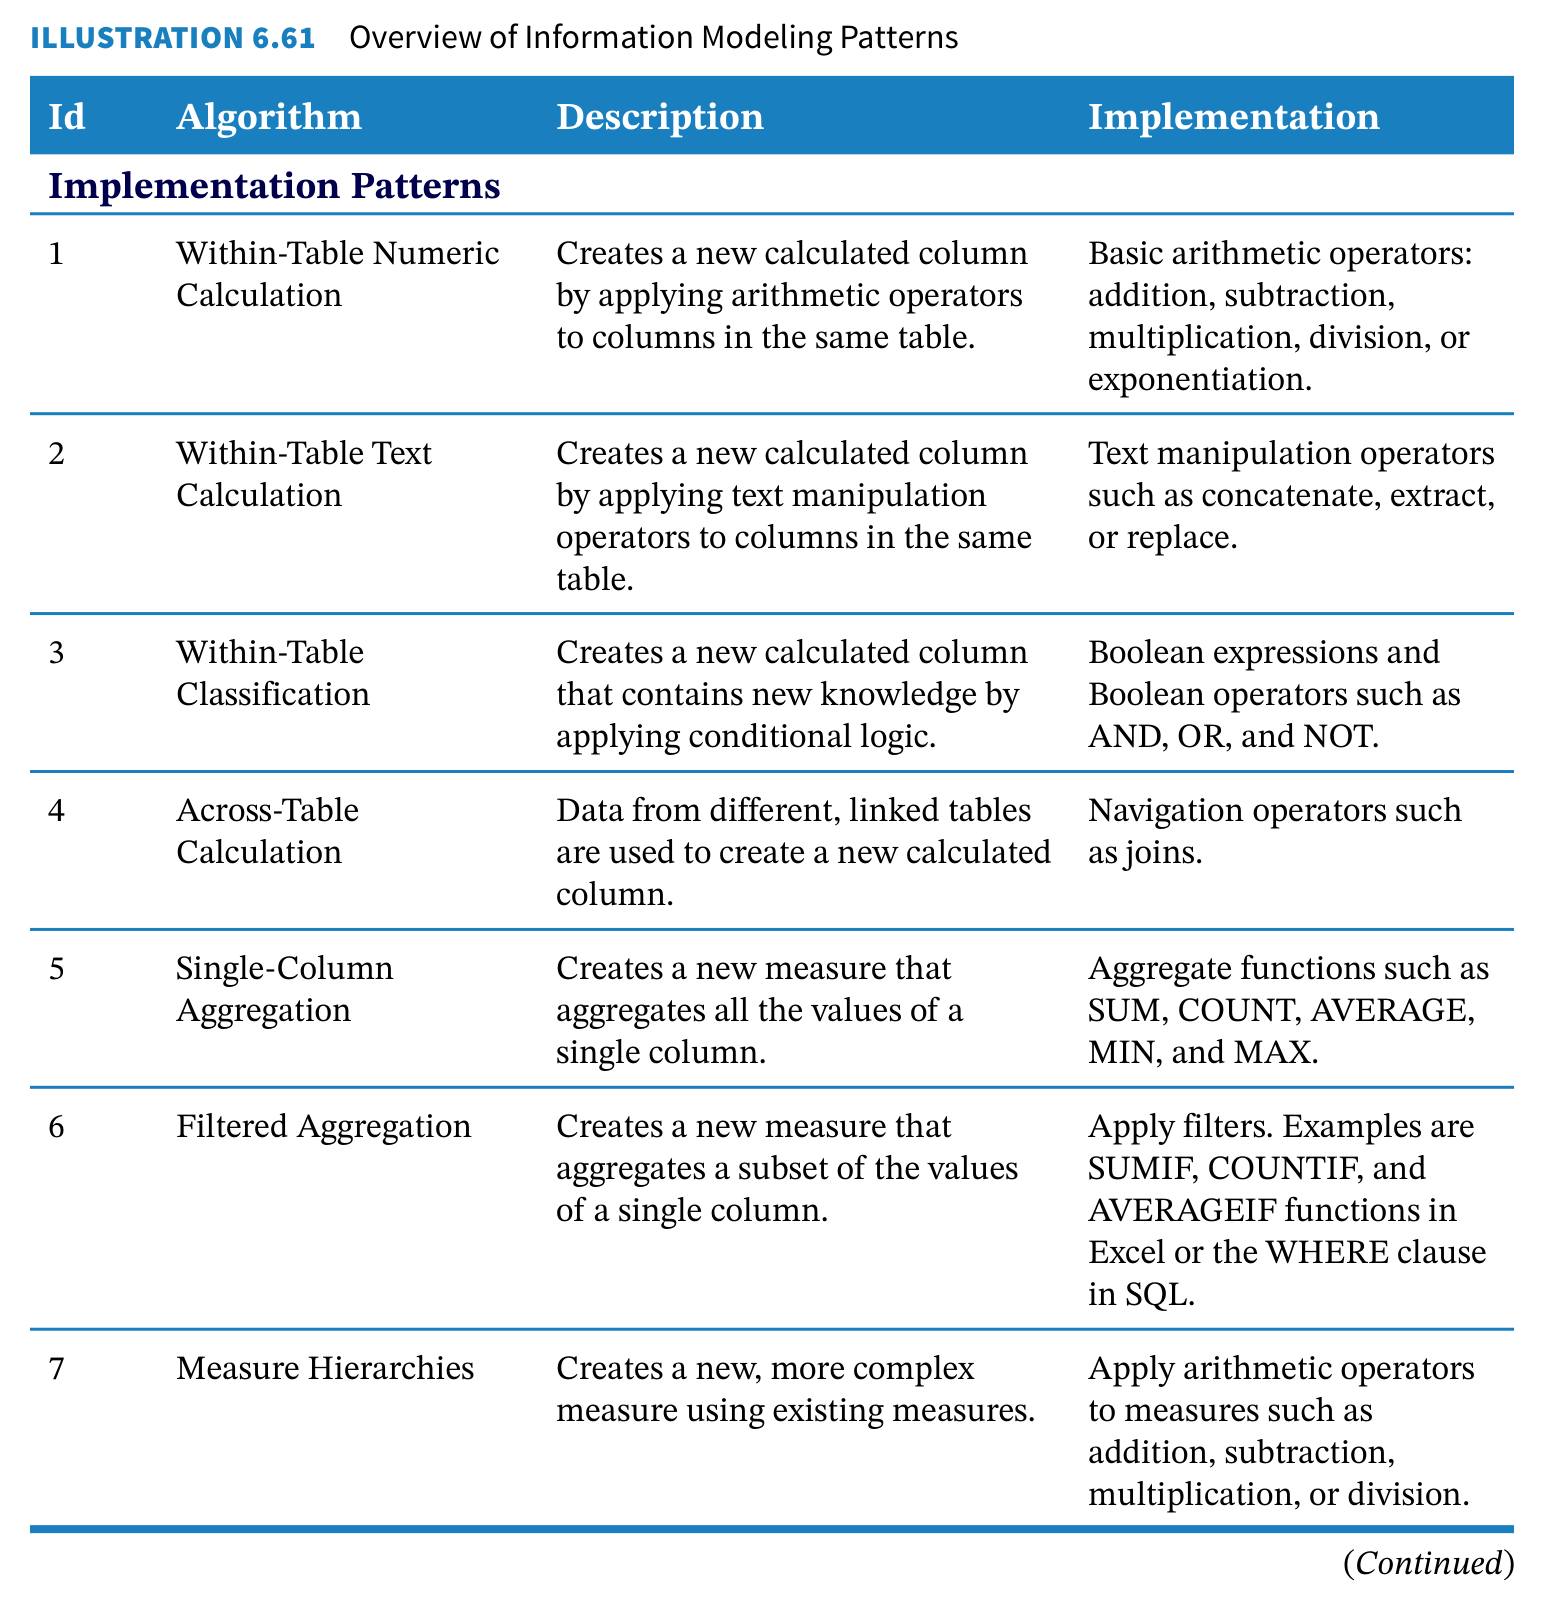
\includegraphics[width=0.95\textwidth,height=0.75\textheight,keepaspectratio]{../textbookForPractice/Figures/Ch_06/ILLUSTRATION 6.61A.png}
    \end{figure}
\end{frame}

\begin{frame}{ILLUSTRATION 6.61B}

    \begin{figure}[h]
        \centering
        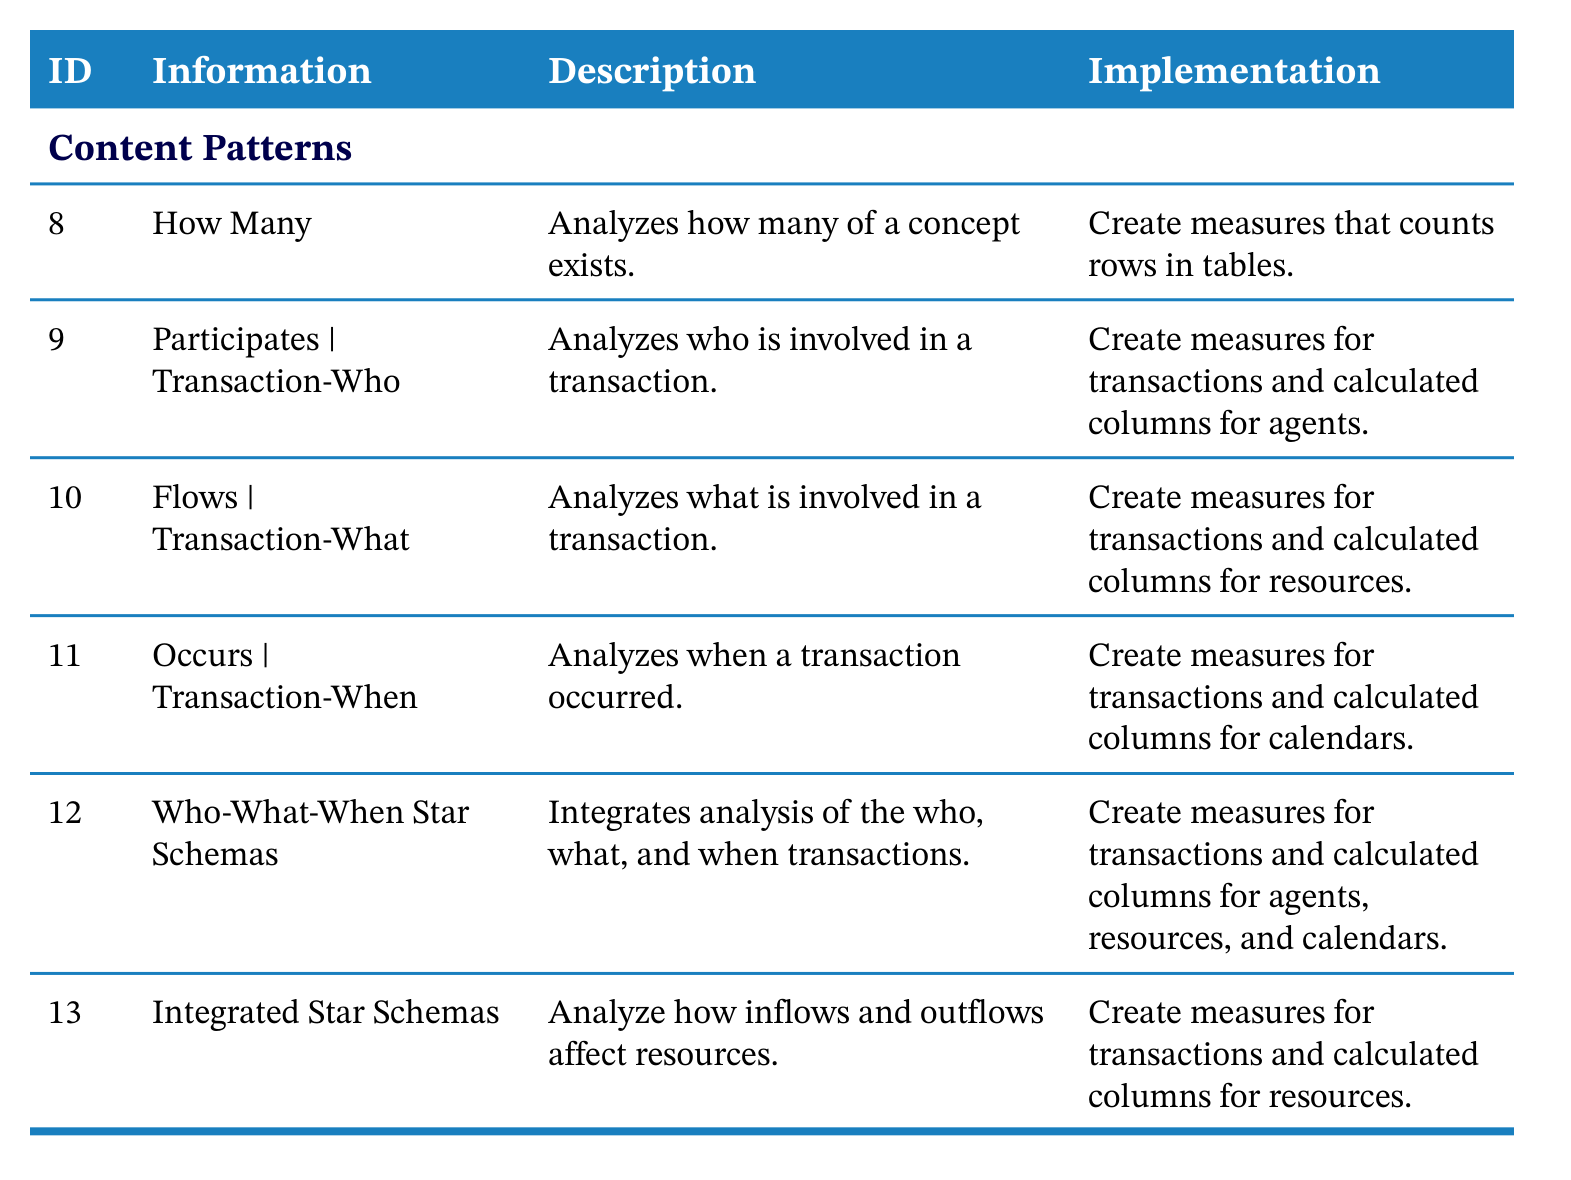
\includegraphics[width=0.95\textwidth,height=0.75\textheight,keepaspectratio]{../textbookForPractice/Figures/Ch_06/ILLUSTRATION 6.61B.png}
    \end{figure}
\end{frame}

\begin{frame}{ILLUSTRATION 6.62}

    \begin{figure}[h]
        \centering
        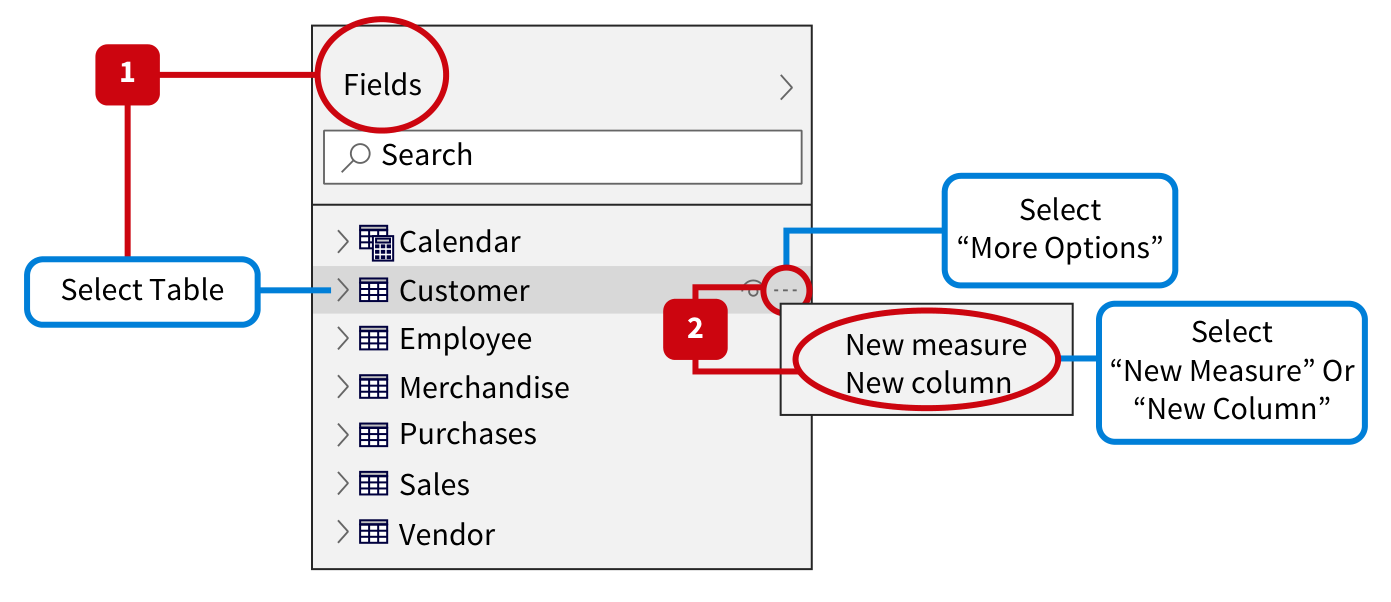
\includegraphics[width=0.95\textwidth,height=0.75\textheight,keepaspectratio]{../textbookForPractice/Figures/Ch_06/ILLUSTRATION 6.62.png}
    \end{figure}
\end{frame}

\begin{frame}{ILLUSTRATION 6.63}

    \begin{figure}[h]
        \centering
        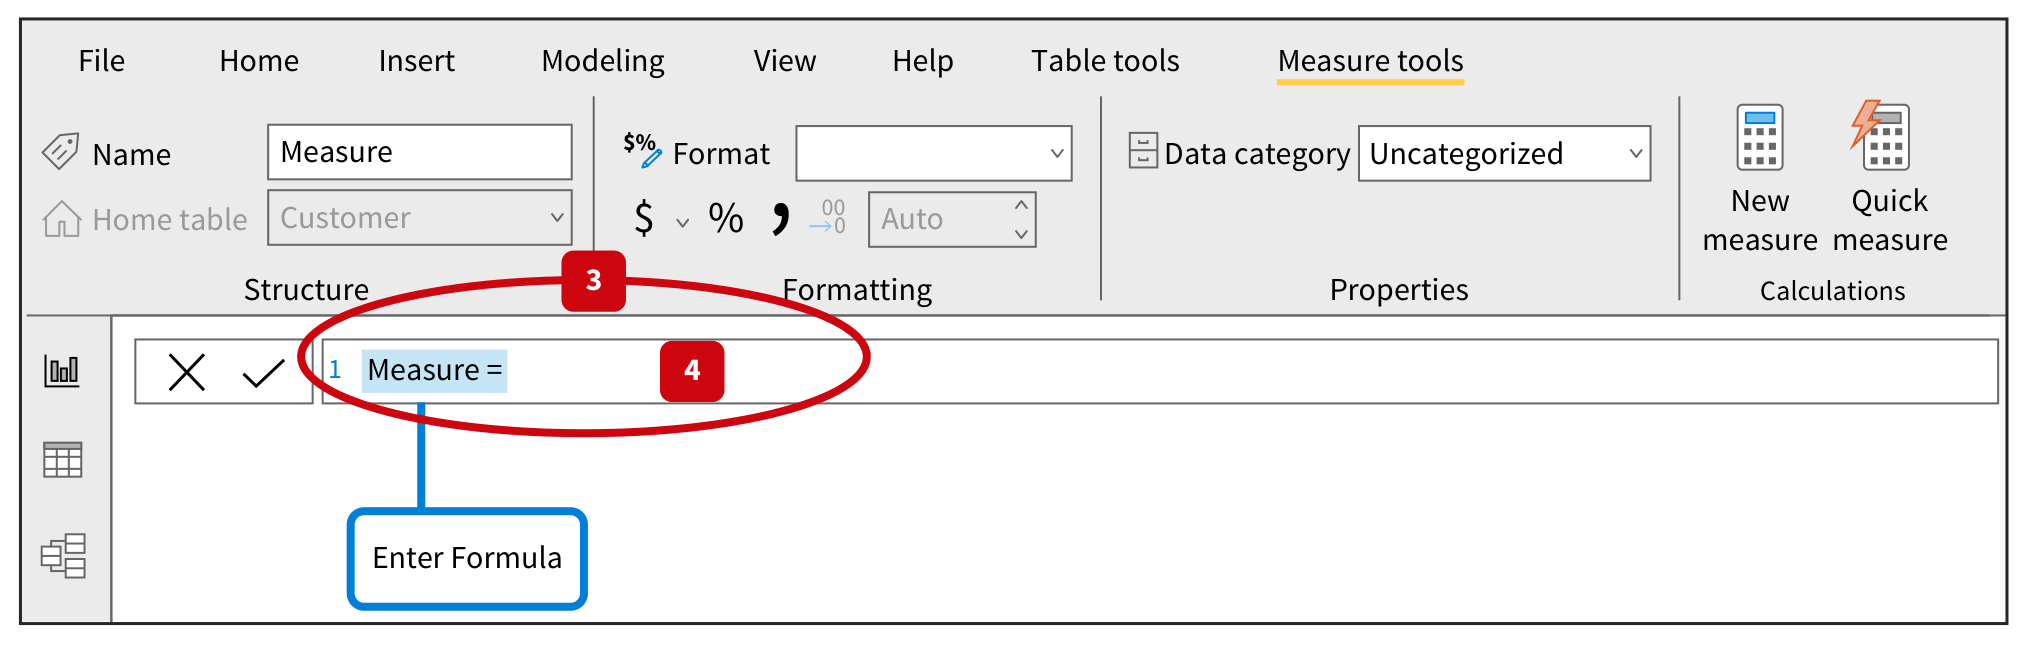
\includegraphics[width=0.95\textwidth,height=0.75\textheight,keepaspectratio]{../textbookForPractice/Figures/Ch_06/ILLUSTRATION 6.63.png}
    \end{figure}
\end{frame}

\begin{frame}{ILLUSTRATION 6.64}

    \begin{figure}[h]
        \centering
        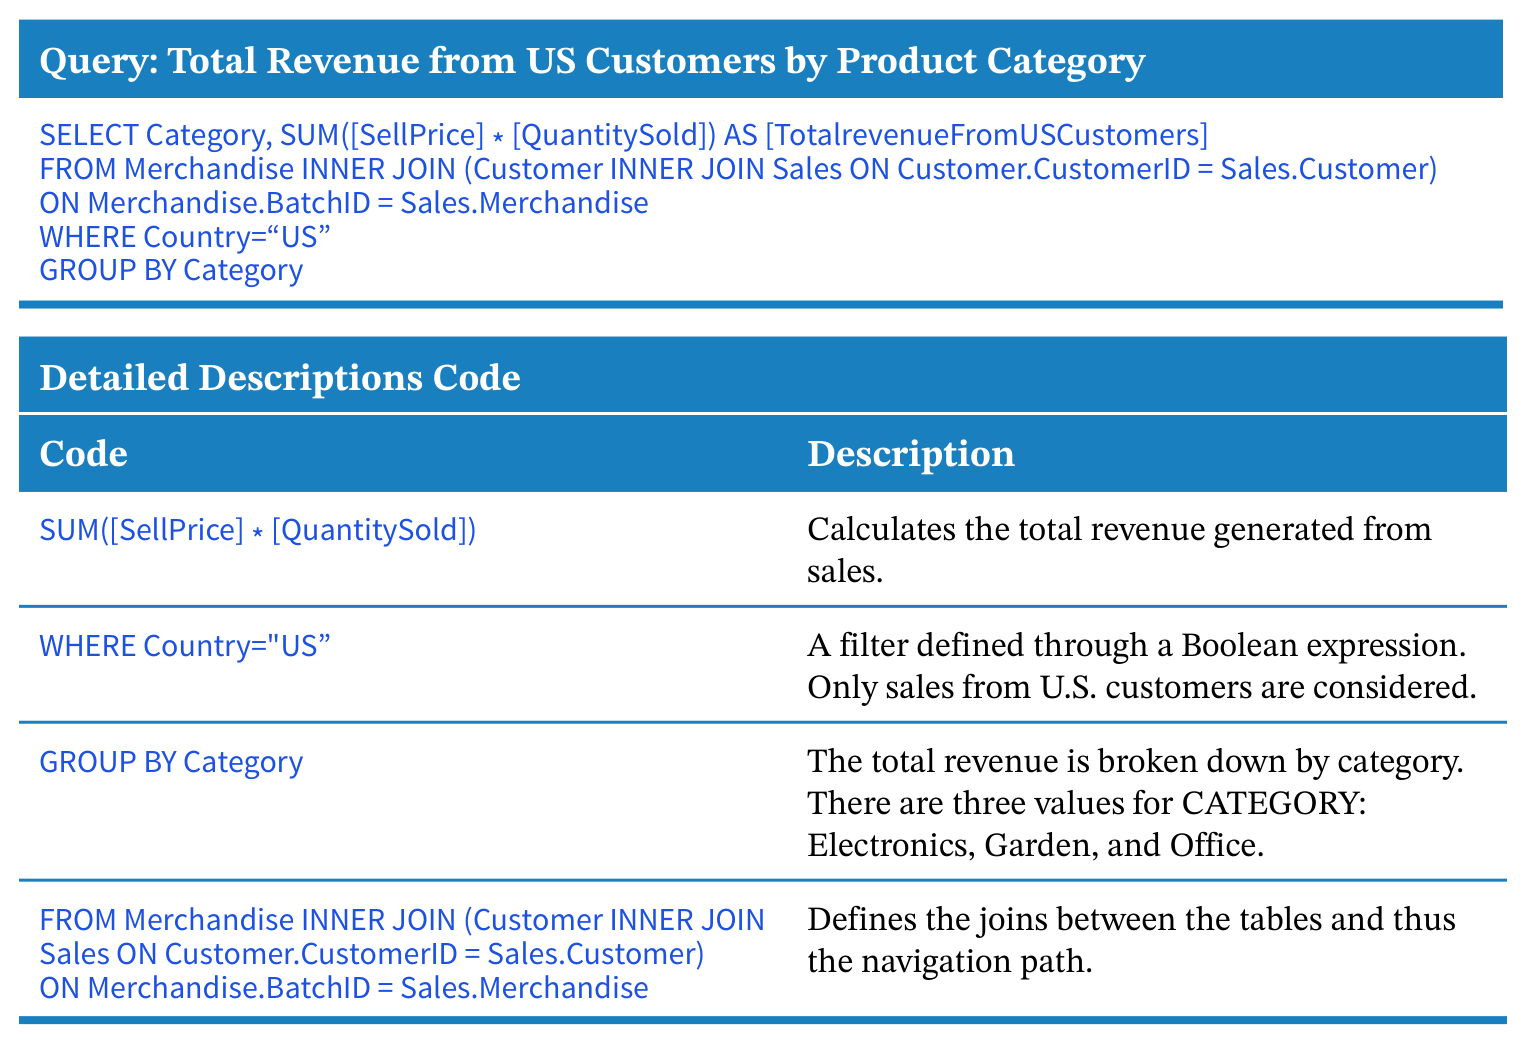
\includegraphics[width=0.95\textwidth,height=0.75\textheight,keepaspectratio]{../textbookForPractice/Figures/Ch_06/ILLUSTRATION 6.64.png}
    \end{figure}
\end{frame}

\begin{frame}{ILLUSTRATION 6.65}

    \begin{figure}[h]
        \centering
        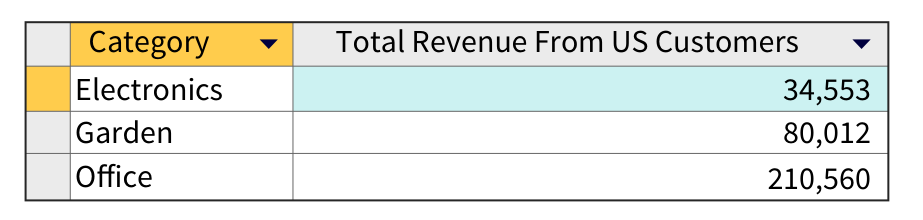
\includegraphics[width=0.95\textwidth,height=0.75\textheight,keepaspectratio]{../textbookForPractice/Figures/Ch_06/ILLUSTRATION 6.65.png}
    \end{figure}
\end{frame}

\begin{frame}{Bài tập Ngắn (Brief Exercises)}
\begin{center}
    \Huge \textbf{Phần Bài tập Ngắn} \\
    \vspace{0.5cm}
    \Large Brief Exercises (BE)
\end{center}
\end{frame}

\begin{frame}{BE 6.5 \& BE 6.11}
    \begin{columns}
        \begin{column}{0.5\textwidth}
            \begin{figure}[h]
                \centering
                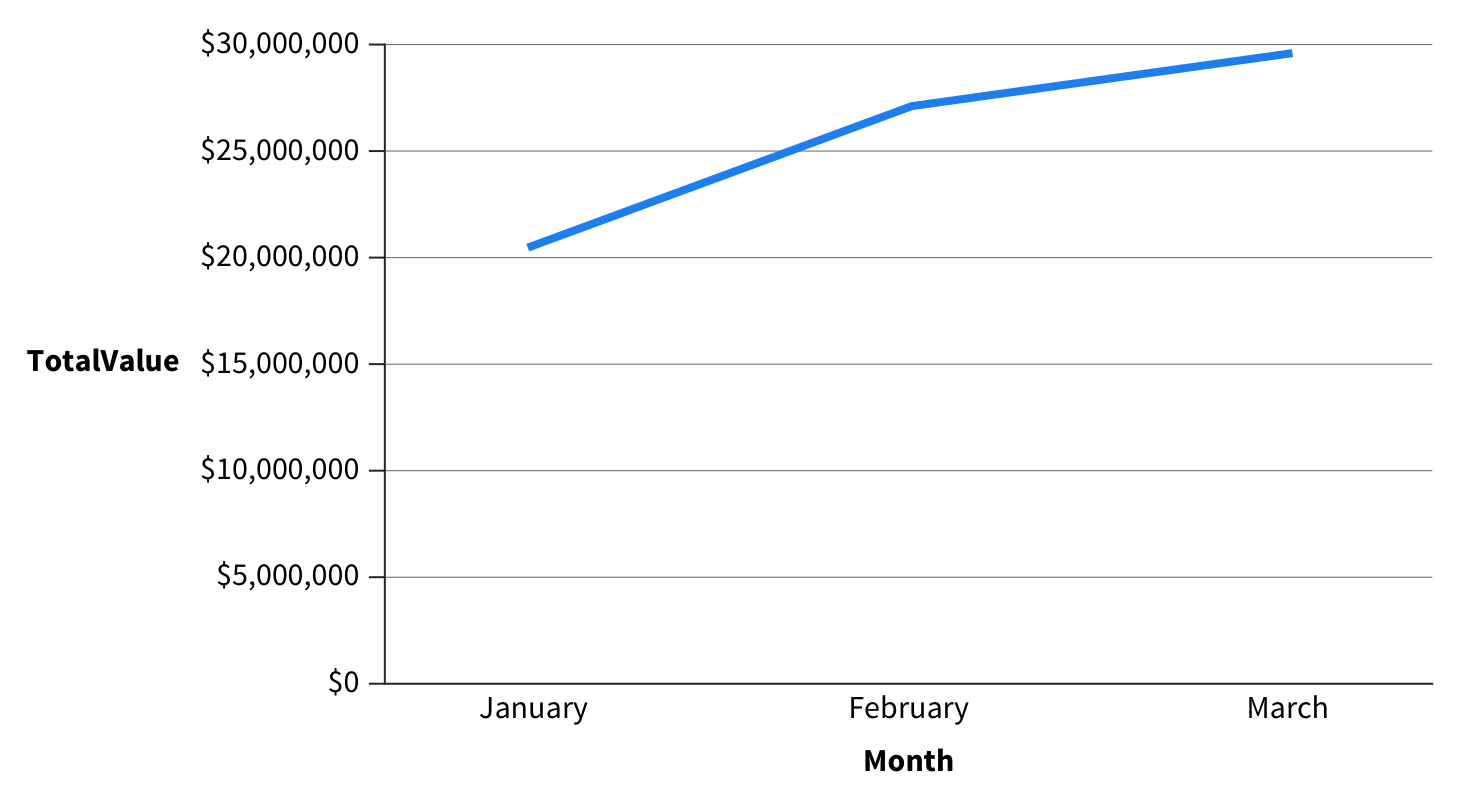
\includegraphics[width=\textwidth,height=0.7\textheight,keepaspectratio]{../textbookForPractice/Figures/Ch_06/BE 6.5.png}
            \end{figure}
        \end{column}
        \begin{column}{0.5\textwidth}
            \begin{figure}[h]
                \centering
                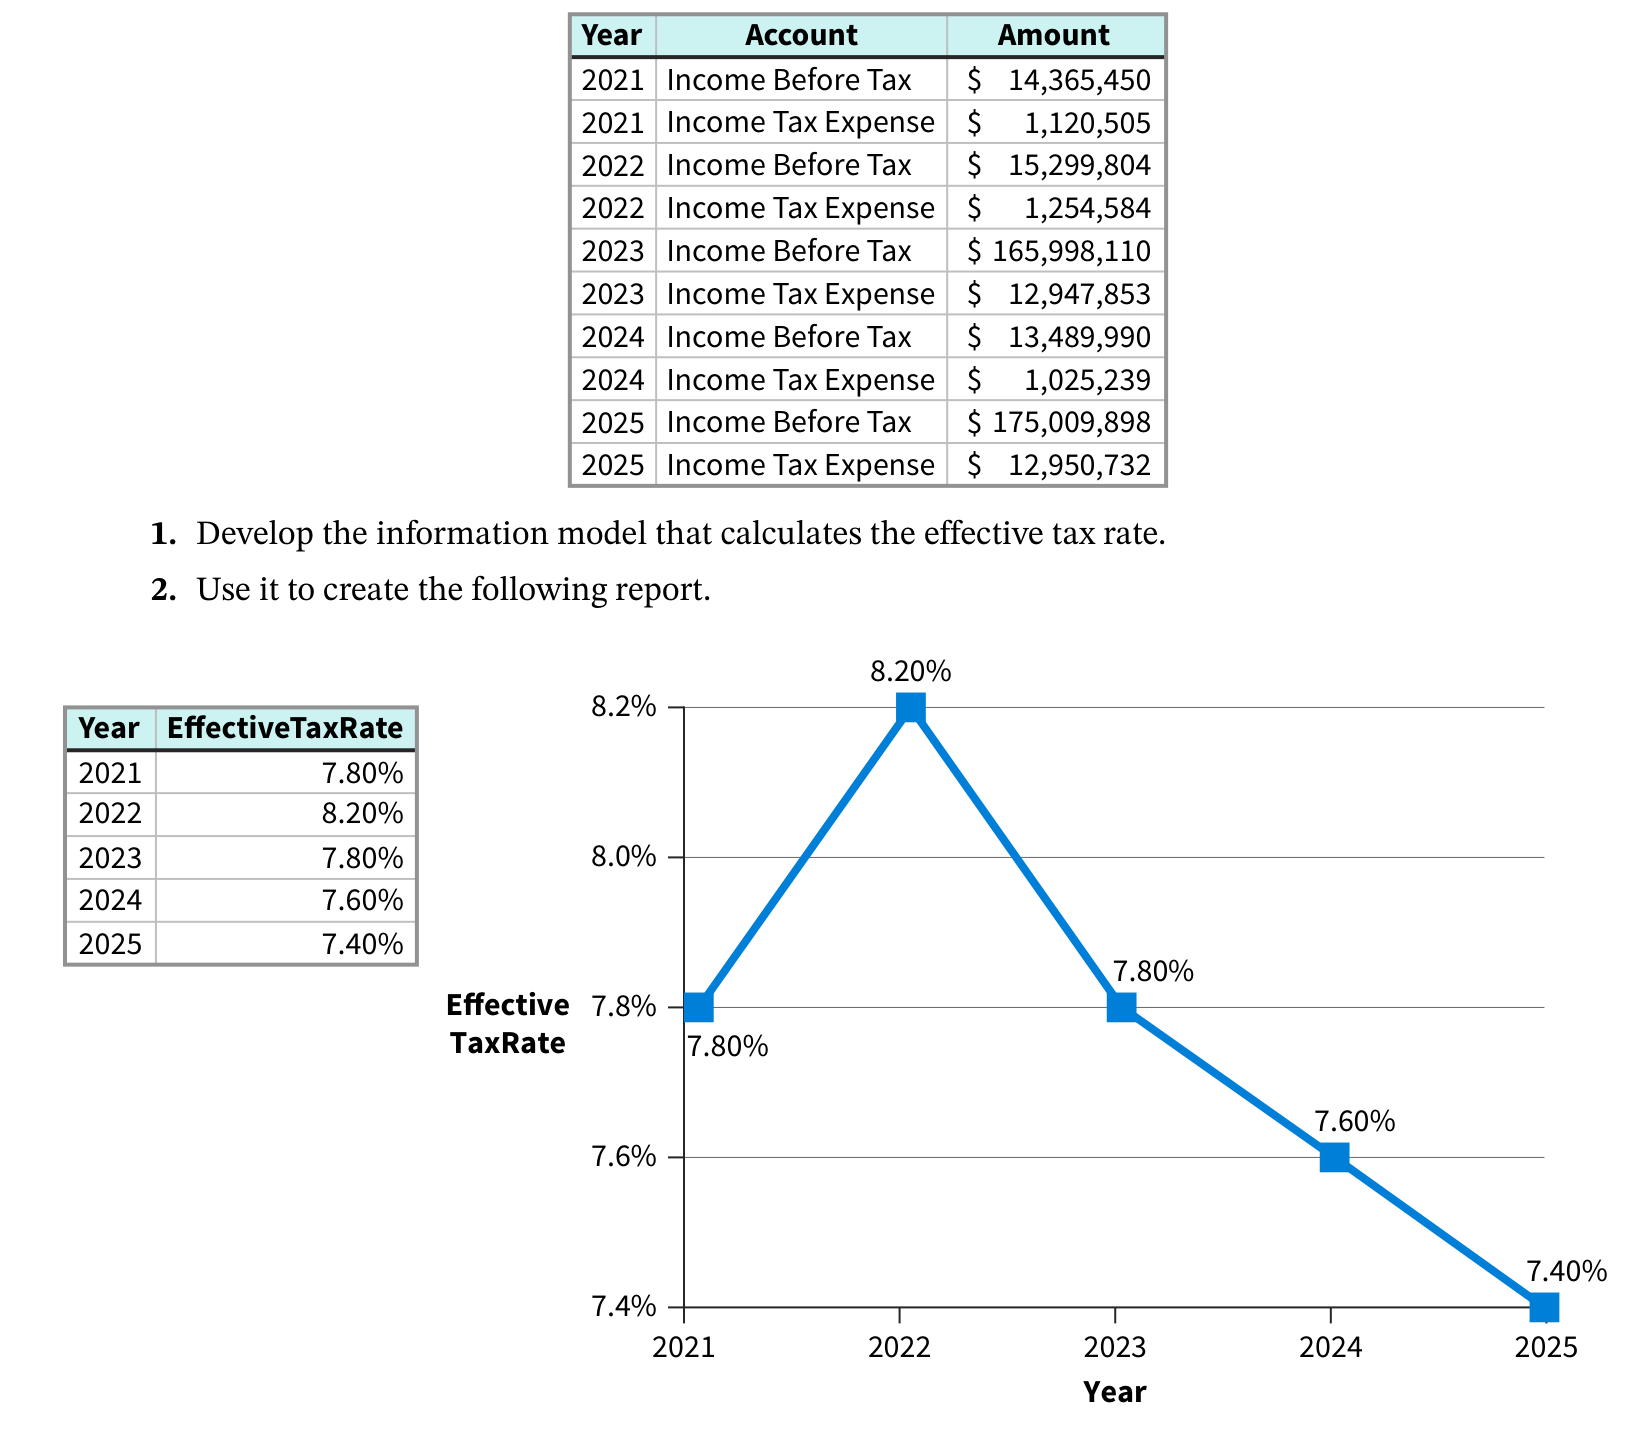
\includegraphics[width=\textwidth,height=0.7\textheight,keepaspectratio]{../textbookForPractice/Figures/Ch_06/BE 6.11.png}
            \end{figure}
        \end{column}
    \end{columns}
\end{frame}

\begin{frame}{BE 6.12 \& BE 6.14}
    \begin{columns}
        \begin{column}{0.5\textwidth}
            \begin{figure}[h]
                \centering
                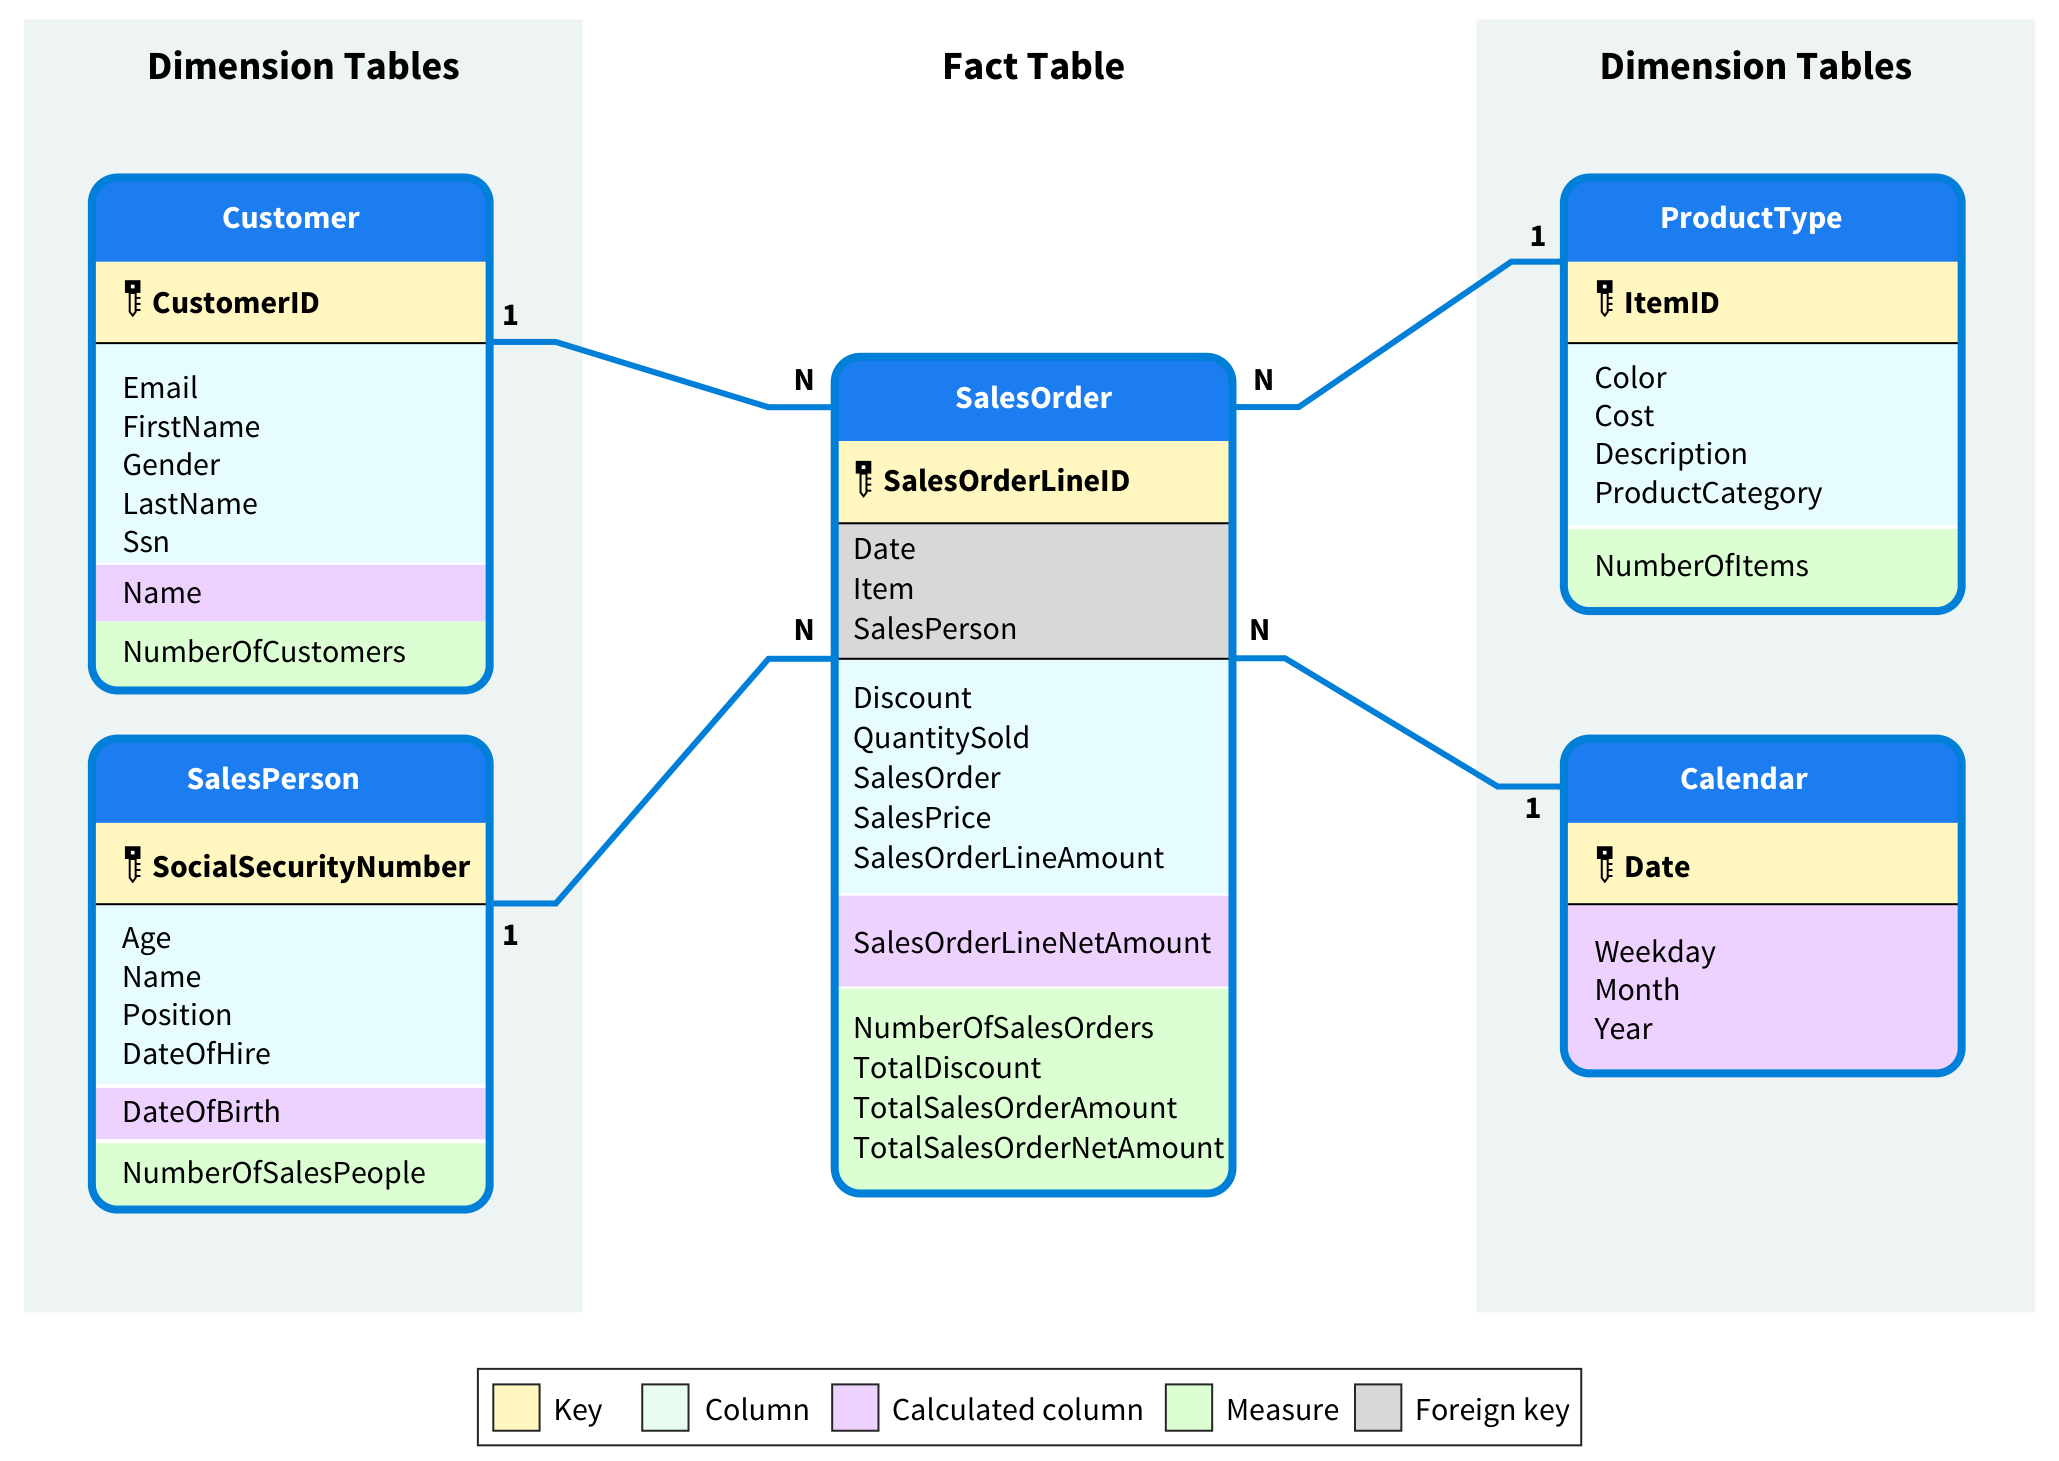
\includegraphics[width=\textwidth,height=0.7\textheight,keepaspectratio]{../textbookForPractice/Figures/Ch_06/BE 6.12.png}
            \end{figure}
        \end{column}
        \begin{column}{0.5\textwidth}
            \begin{figure}[h]
                \centering
                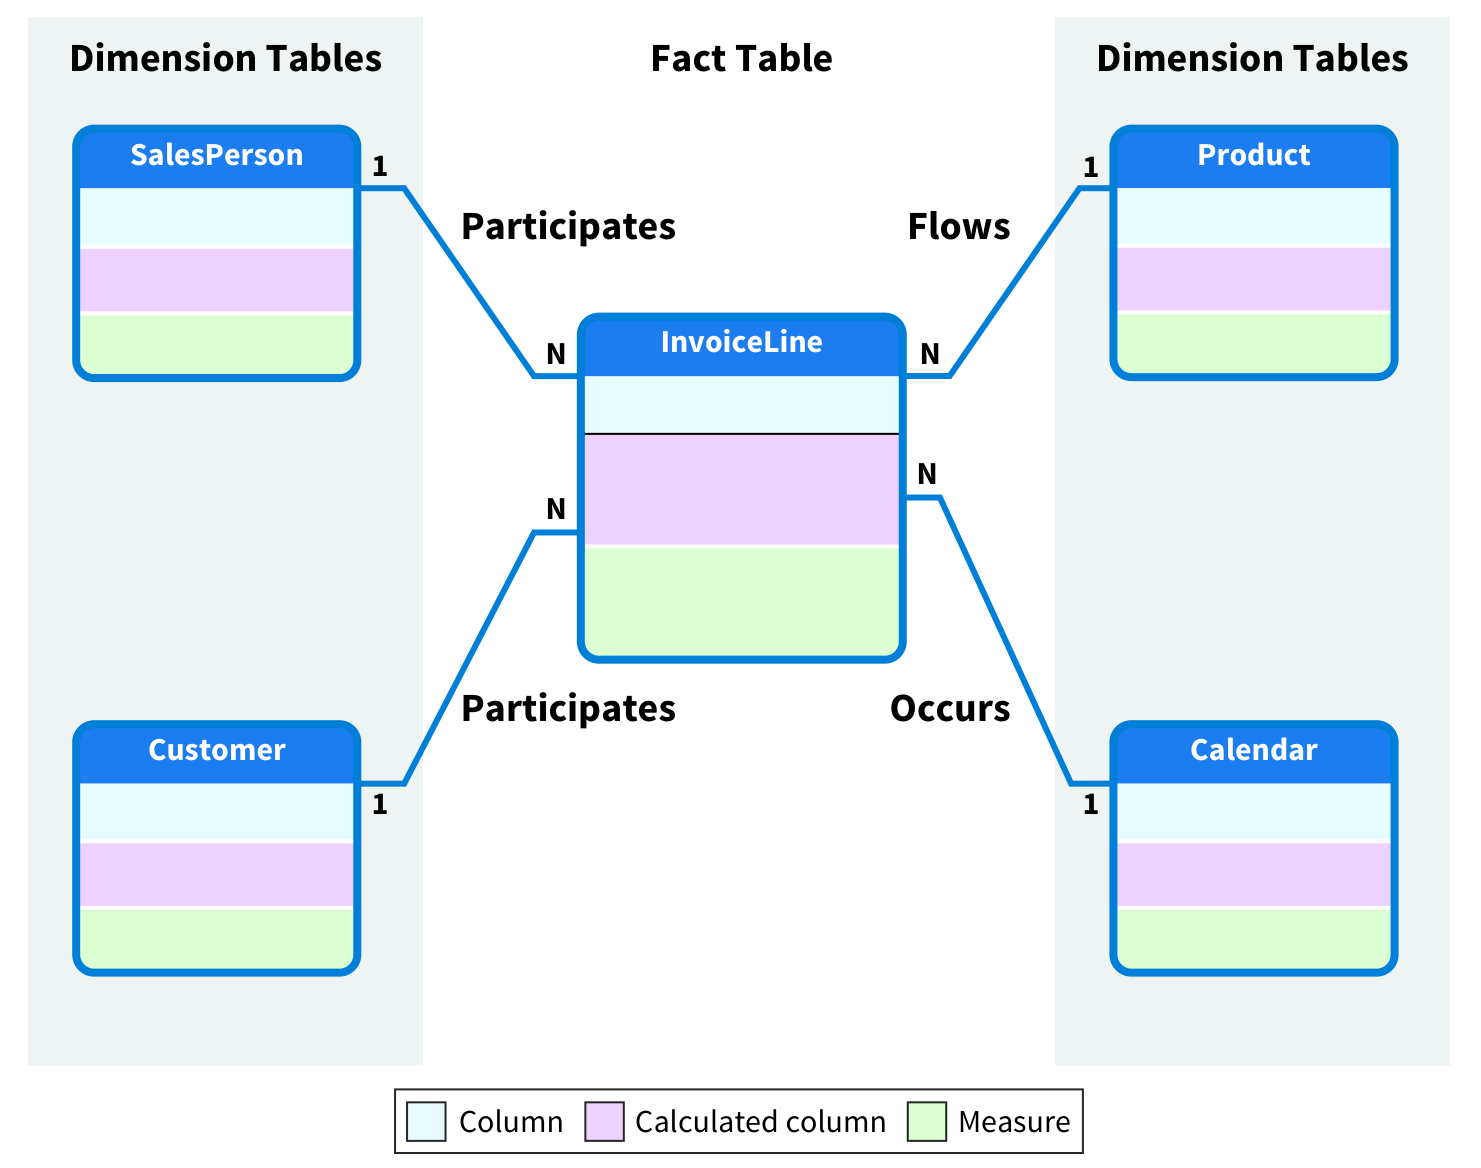
\includegraphics[width=\textwidth,height=0.7\textheight,keepaspectratio]{../textbookForPractice/Figures/Ch_06/BE 6.14.png}
            \end{figure}
        \end{column}
    \end{columns}
\end{frame}

\begin{frame}{BE 6.15}

    \begin{figure}[h]
        \centering
        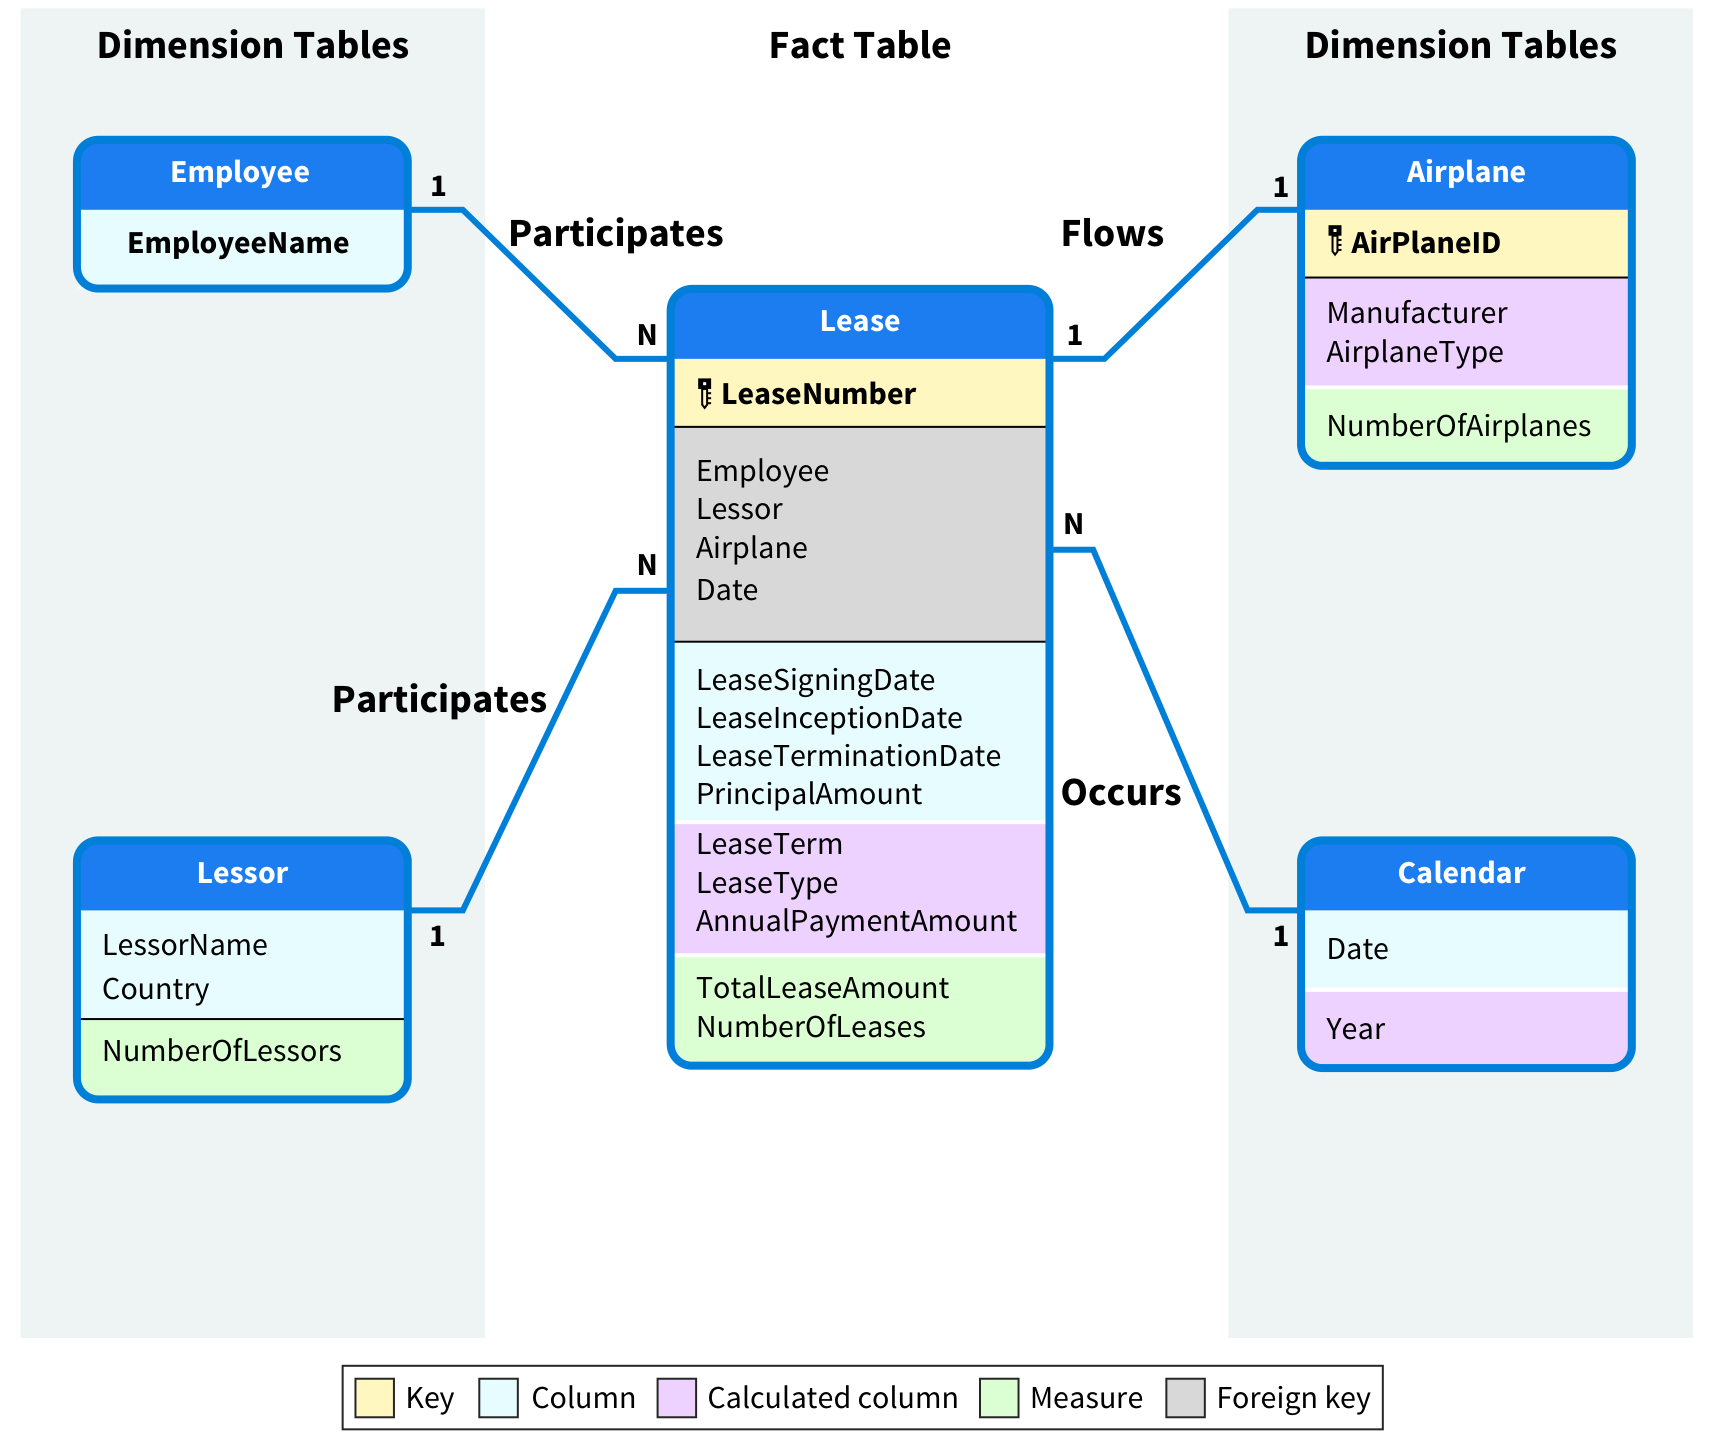
\includegraphics[width=0.95\textwidth,height=0.75\textheight,keepaspectratio]{../textbookForPractice/Figures/Ch_06/BE 6.15.png}
    \end{figure}
\end{frame}

\begin{frame}{Bài tập (Exercises)}
\begin{center}
    \Huge \textbf{Phần Bài tập} \\
    \vspace{0.5cm}
    \Large Exercises (EX)
\end{center}
\end{frame}

\begin{frame}{EX 6.2 \& EX 6.3}
    \begin{columns}
        \begin{column}{0.5\textwidth}
            \begin{figure}[h]
                \centering
                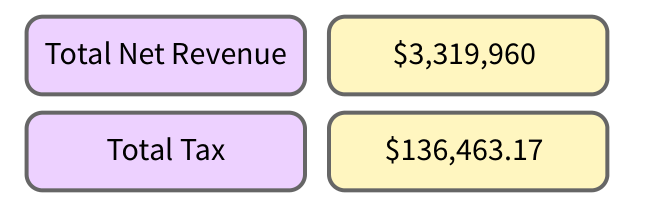
\includegraphics[width=\textwidth,height=0.7\textheight,keepaspectratio]{../textbookForPractice/Figures/Ch_06/EX 6.2.png}
            \end{figure}
        \end{column}
        \begin{column}{0.5\textwidth}
            \begin{figure}[h]
                \centering
                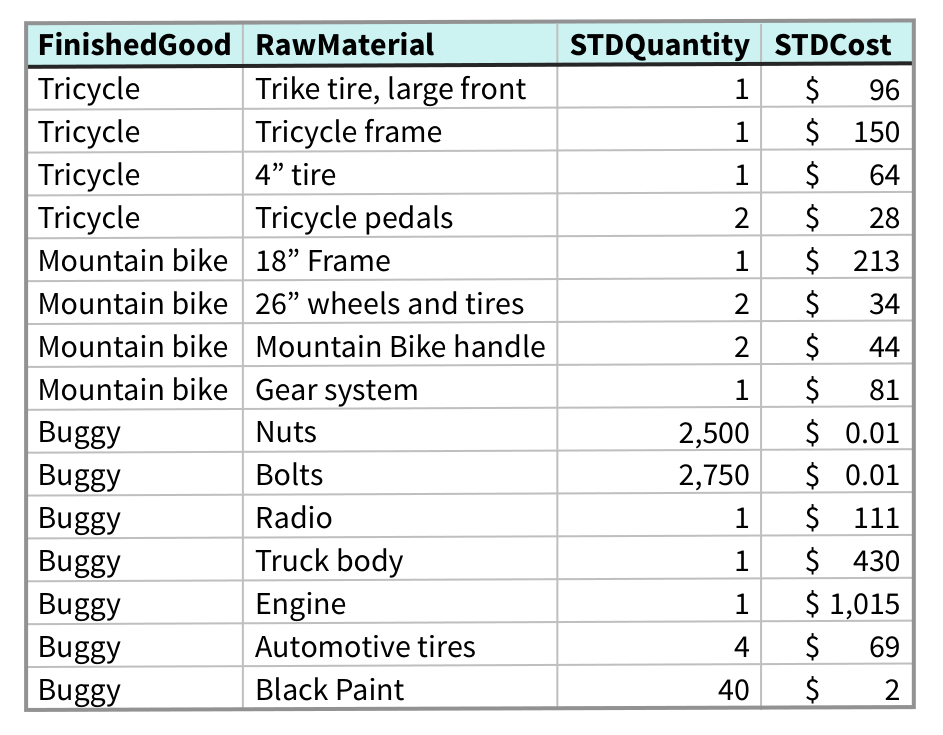
\includegraphics[width=\textwidth,height=0.7\textheight,keepaspectratio]{../textbookForPractice/Figures/Ch_06/EX 6.3.png}
            \end{figure}
        \end{column}
    \end{columns}
\end{frame}

\begin{frame}{EX 6.4A \& EX 6.4B}
    \begin{columns}
        \begin{column}{0.5\textwidth}
            \begin{figure}[h]
                \centering
                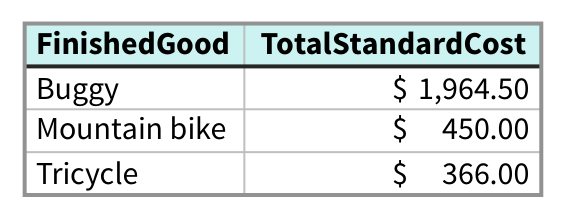
\includegraphics[width=\textwidth,height=0.7\textheight,keepaspectratio]{../textbookForPractice/Figures/Ch_06/EX 6.4A.png}
            \end{figure}
        \end{column}
        \begin{column}{0.5\textwidth}
            \begin{figure}[h]
                \centering
                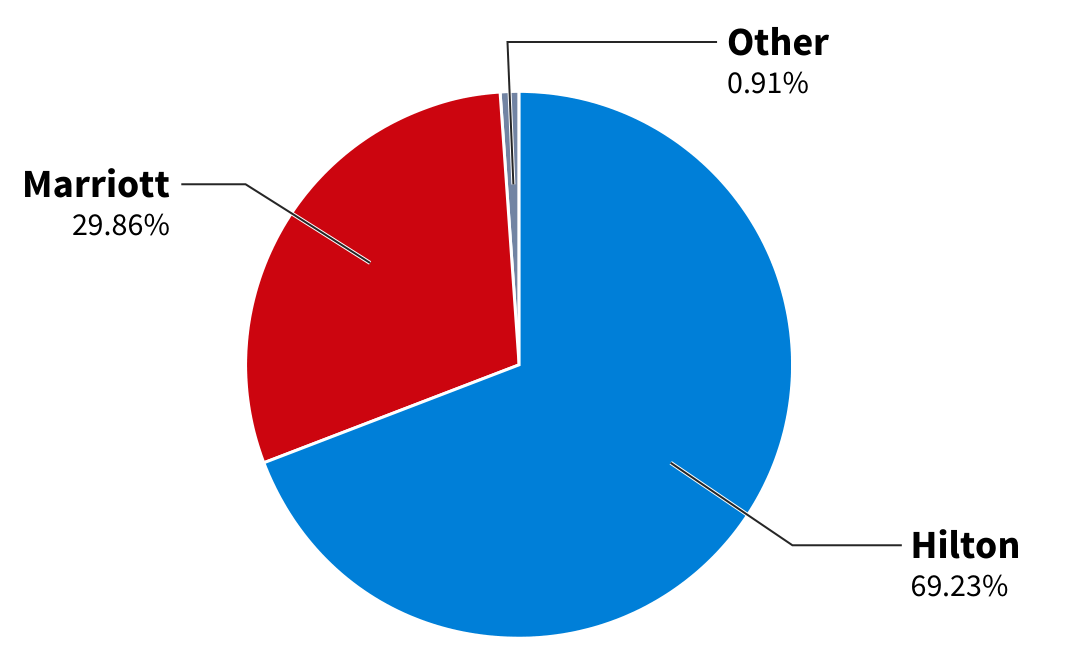
\includegraphics[width=\textwidth,height=0.7\textheight,keepaspectratio]{../textbookForPractice/Figures/Ch_06/EX 6.4B.png}
            \end{figure}
        \end{column}
    \end{columns}
\end{frame}

\begin{frame}{EX 6.5 \& EX 6.5\_1}
    \begin{columns}
        \begin{column}{0.5\textwidth}
            \begin{figure}[h]
                \centering
                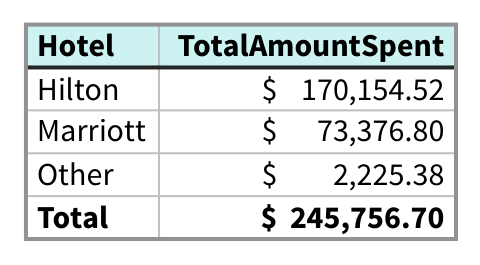
\includegraphics[width=\textwidth,height=0.7\textheight,keepaspectratio]{../textbookForPractice/Figures/Ch_06/EX 6.5.png}
            \end{figure}
        \end{column}
        \begin{column}{0.5\textwidth}
            \begin{figure}[h]
                \centering
                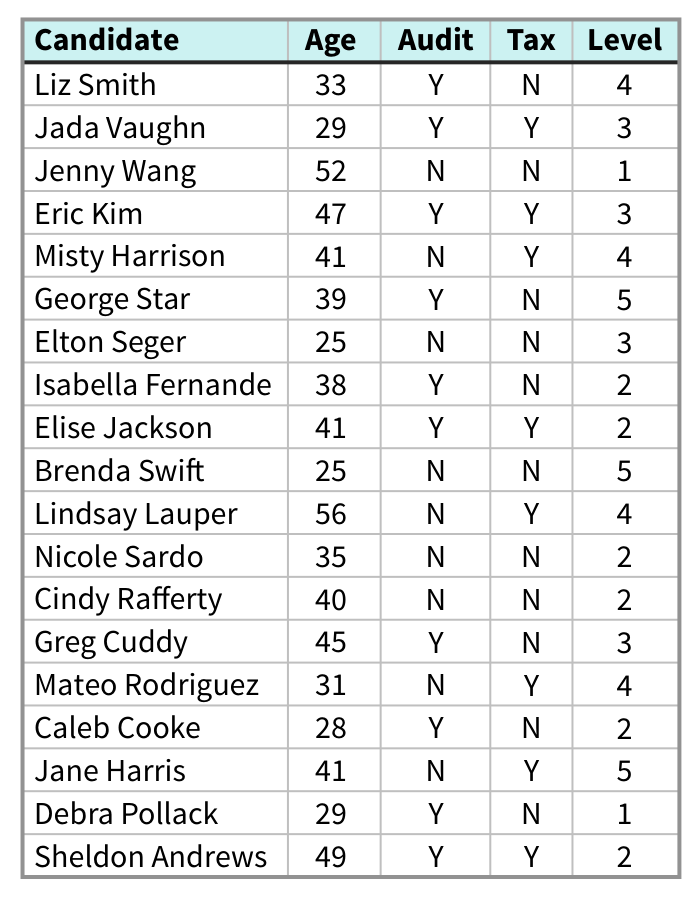
\includegraphics[width=\textwidth,height=0.7\textheight,keepaspectratio]{../textbookForPractice/Figures/Ch_06/EX 6.5_1.png}
            \end{figure}
        \end{column}
    \end{columns}
\end{frame}

\begin{frame}{EX 6.7A \& EX 6.7B}
    \begin{columns}
        \begin{column}{0.5\textwidth}
            \begin{figure}[h]
                \centering
                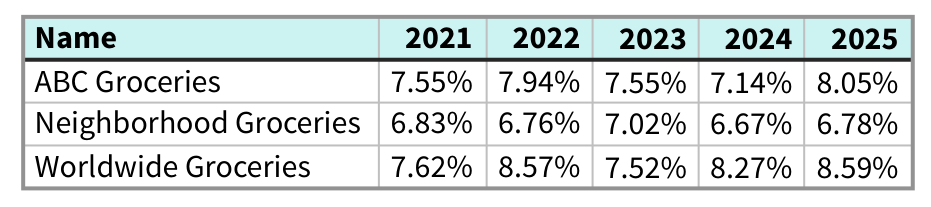
\includegraphics[width=\textwidth,height=0.7\textheight,keepaspectratio]{../textbookForPractice/Figures/Ch_06/EX 6.7A.png}
            \end{figure}
        \end{column}
        \begin{column}{0.5\textwidth}
            \begin{figure}[h]
                \centering
                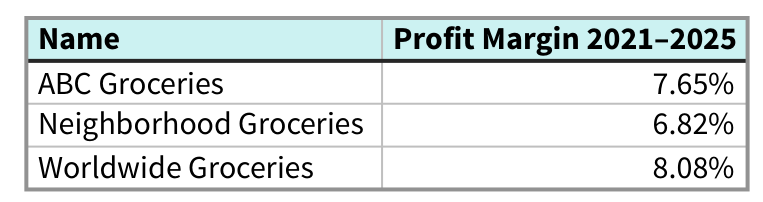
\includegraphics[width=\textwidth,height=0.7\textheight,keepaspectratio]{../textbookForPractice/Figures/Ch_06/EX 6.7B.png}
            \end{figure}
        \end{column}
    \end{columns}
\end{frame}

\begin{frame}{EX 6.9 \& EX 6.10}
    \begin{columns}
        \begin{column}{0.5\textwidth}
            \begin{figure}[h]
                \centering
                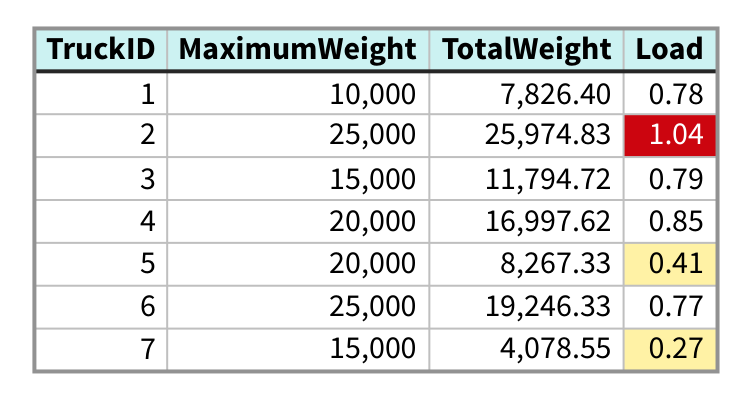
\includegraphics[width=\textwidth,height=0.7\textheight,keepaspectratio]{../textbookForPractice/Figures/Ch_06/EX 6.9.png}
            \end{figure}
        \end{column}
        \begin{column}{0.5\textwidth}
            \begin{figure}[h]
                \centering
                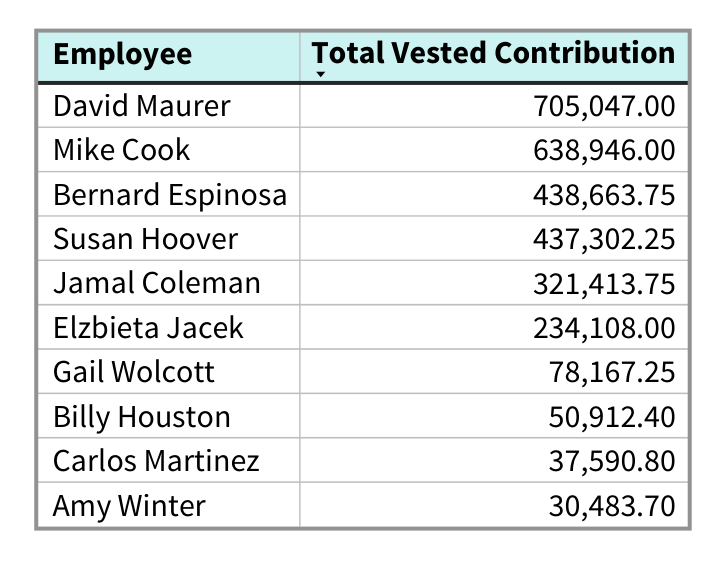
\includegraphics[width=\textwidth,height=0.7\textheight,keepaspectratio]{../textbookForPractice/Figures/Ch_06/EX 6.10.png}
            \end{figure}
        \end{column}
    \end{columns}
\end{frame}

\begin{frame}{EX 6.11A \& EX 6.11B}
    \begin{columns}
        \begin{column}{0.5\textwidth}
            \begin{figure}[h]
                \centering
                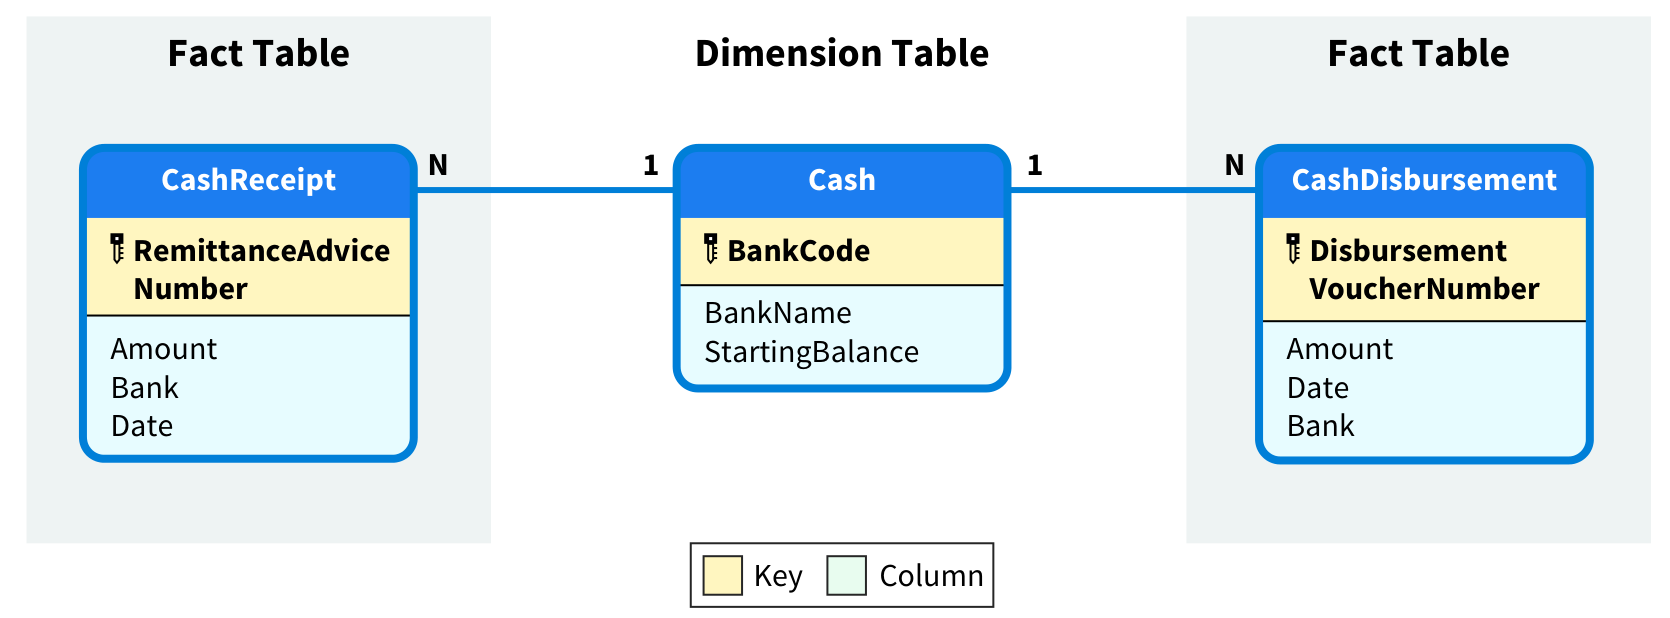
\includegraphics[width=\textwidth,height=0.7\textheight,keepaspectratio]{../textbookForPractice/Figures/Ch_06/EX 6.11A.png}
            \end{figure}
        \end{column}
        \begin{column}{0.5\textwidth}
            \begin{figure}[h]
                \centering
                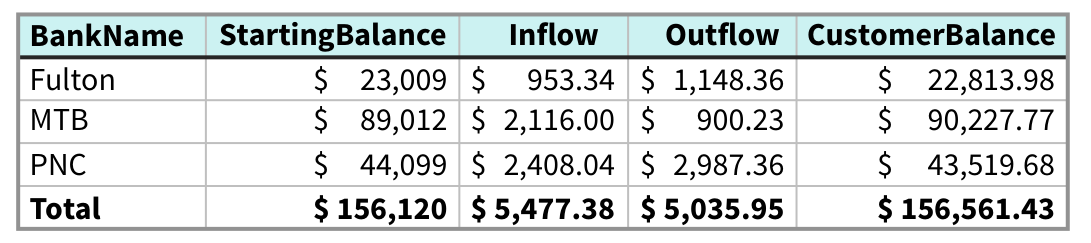
\includegraphics[width=\textwidth,height=0.7\textheight,keepaspectratio]{../textbookForPractice/Figures/Ch_06/EX 6.11B.png}
            \end{figure}
        \end{column}
    \end{columns}
\end{frame}

\begin{frame}{EX 6.12 \& EX 6.13A}
    \begin{columns}
        \begin{column}{0.5\textwidth}
            \begin{figure}[h]
                \centering
                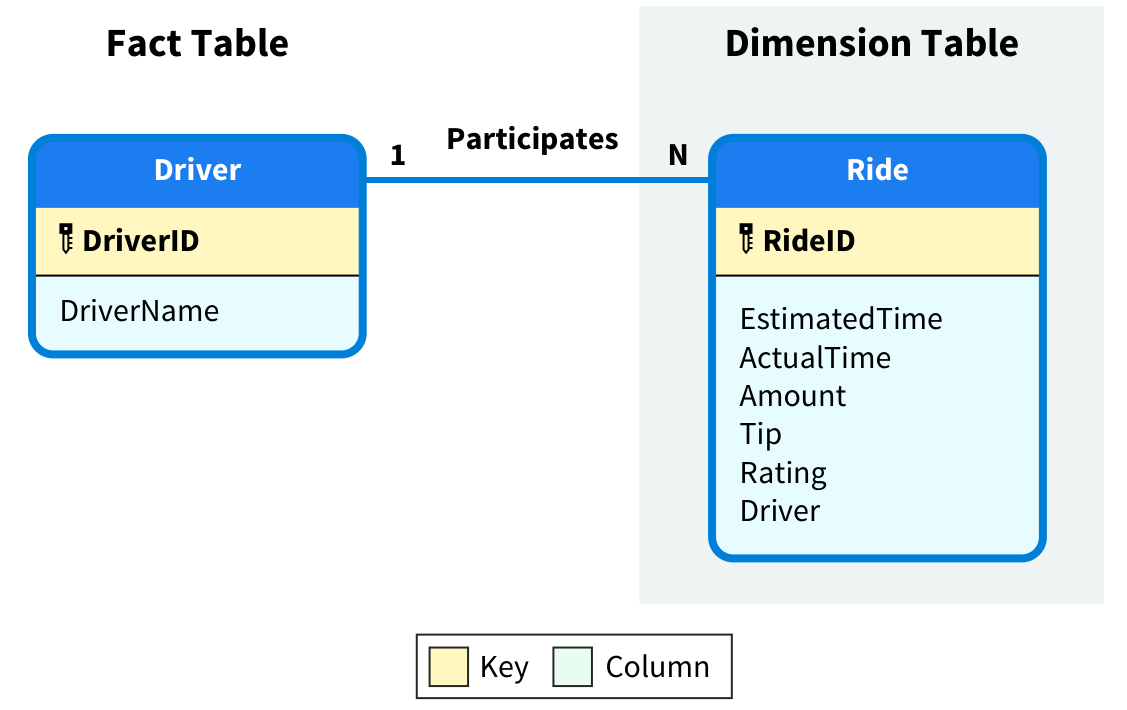
\includegraphics[width=\textwidth,height=0.7\textheight,keepaspectratio]{../textbookForPractice/Figures/Ch_06/EX 6.12.png}
            \end{figure}
        \end{column}
        \begin{column}{0.5\textwidth}
            \begin{figure}[h]
                \centering
                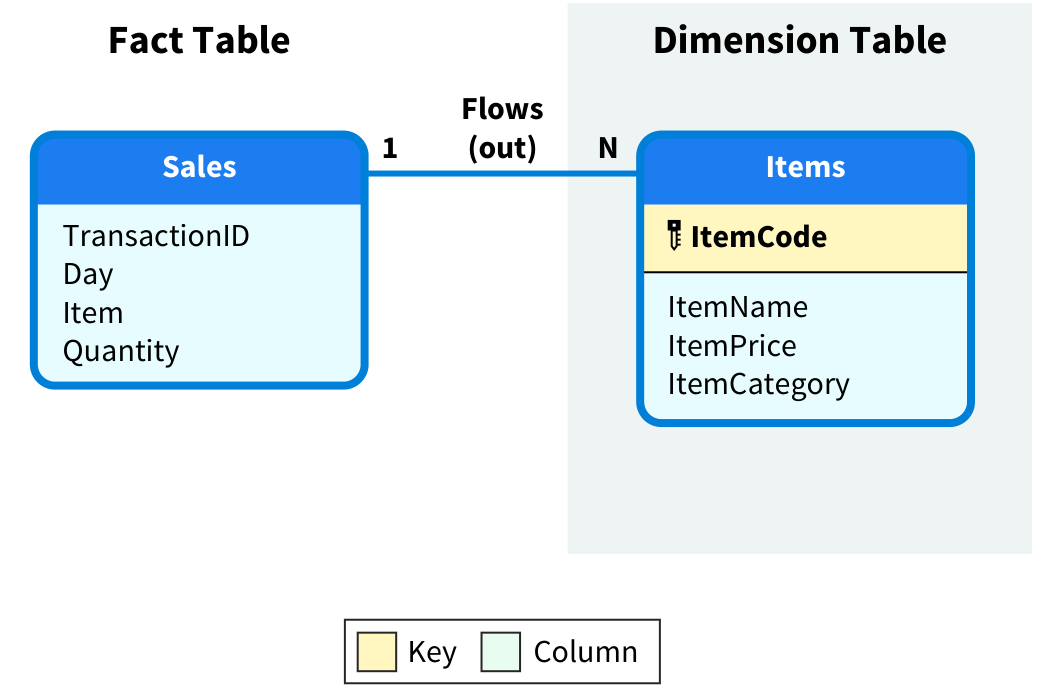
\includegraphics[width=\textwidth,height=0.7\textheight,keepaspectratio]{../textbookForPractice/Figures/Ch_06/EX 6.13A.png}
            \end{figure}
        \end{column}
    \end{columns}
\end{frame}

\begin{frame}{EX 6.13B}

    \begin{figure}[h]
        \centering
        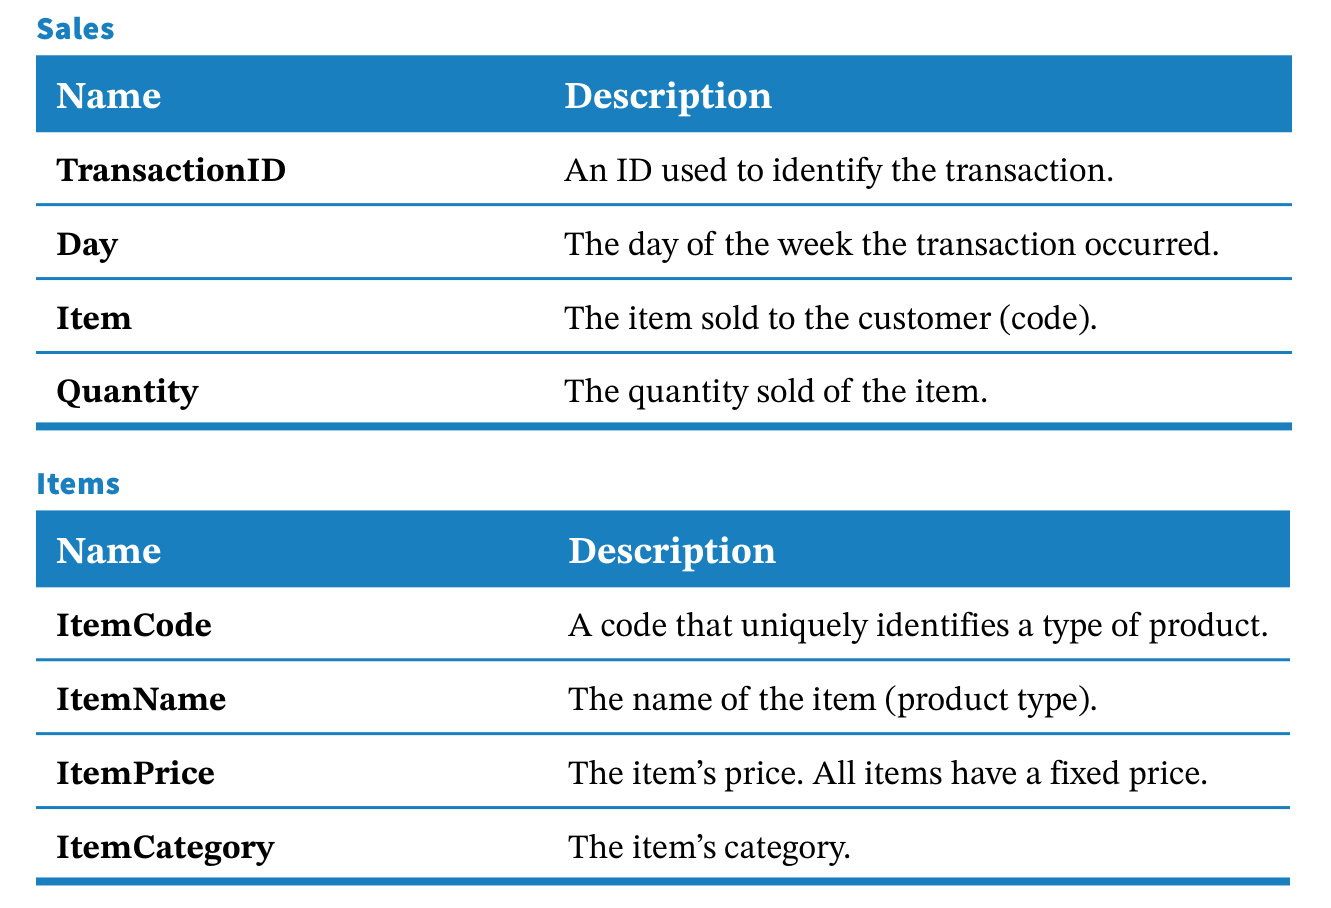
\includegraphics[width=0.95\textwidth,height=0.75\textheight,keepaspectratio]{../textbookForPractice/Figures/Ch_06/EX 6.13B.png}
    \end{figure}
\end{frame}

\begin{frame}{Tình huống Ứng dụng (PAC)}
\begin{center}
    \Huge \textbf{Tình huống Ứng dụng Chuyên môn} \\
    \vspace{0.5cm}
    \Large Professional Application Cases (PAC)
\end{center}
\end{frame}

\begin{frame}{PAC 6.1 \& PAC 6.4}
    \begin{columns}
        \begin{column}{0.5\textwidth}
            \begin{figure}[h]
                \centering
                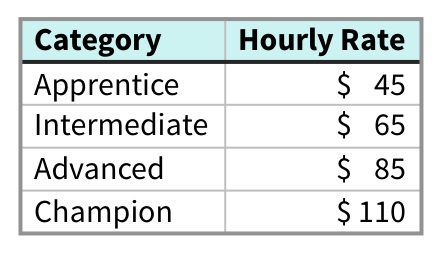
\includegraphics[width=\textwidth,height=0.7\textheight,keepaspectratio]{../textbookForPractice/Figures/Ch_06/PAC 6.1.png}
            \end{figure}
        \end{column}
        \begin{column}{0.5\textwidth}
            \begin{figure}[h]
                \centering
                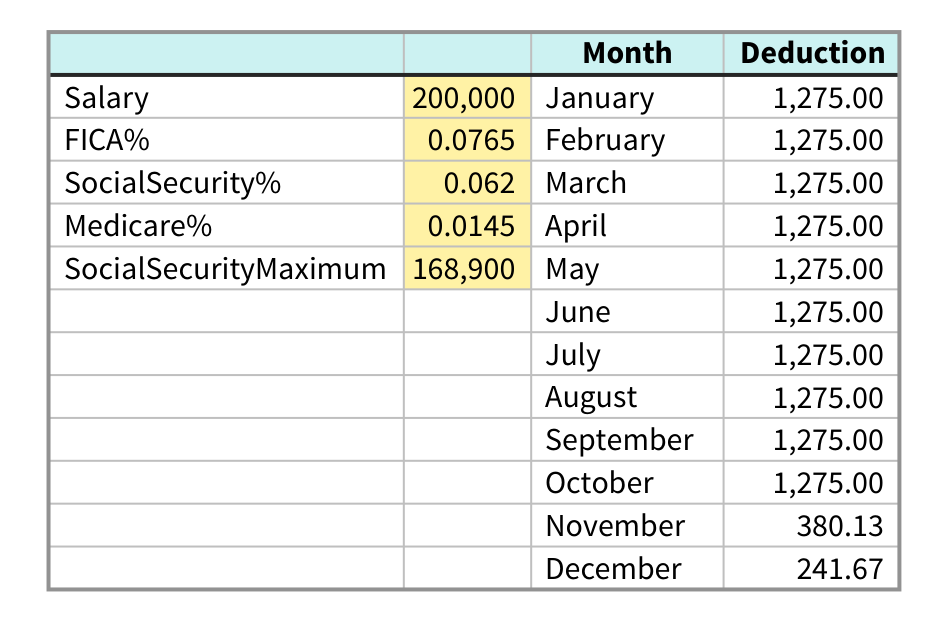
\includegraphics[width=\textwidth,height=0.7\textheight,keepaspectratio]{../textbookForPractice/Figures/Ch_06/PAC 6.4.png}
            \end{figure}
        \end{column}
    \end{columns}
\end{frame}

\begin{frame}{LO 1.4}

    \begin{figure}[h]
        \centering
        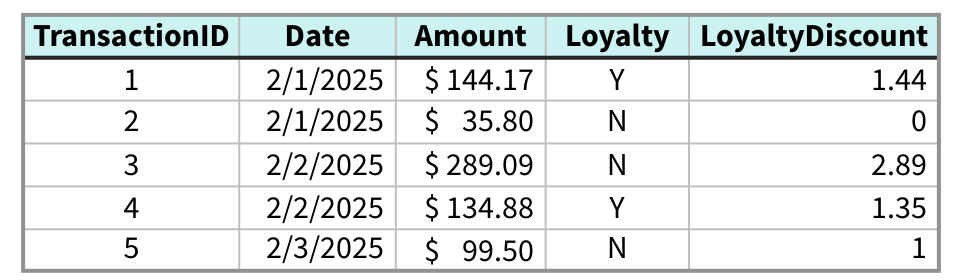
\includegraphics[width=0.95\textwidth,height=0.75\textheight,keepaspectratio]{../textbookForPractice/Figures/Ch_06/LO 1.4.png}
    \end{figure}
\end{frame}

\begin{frame}{LO 1.5}

    \begin{figure}[h]
        \centering
        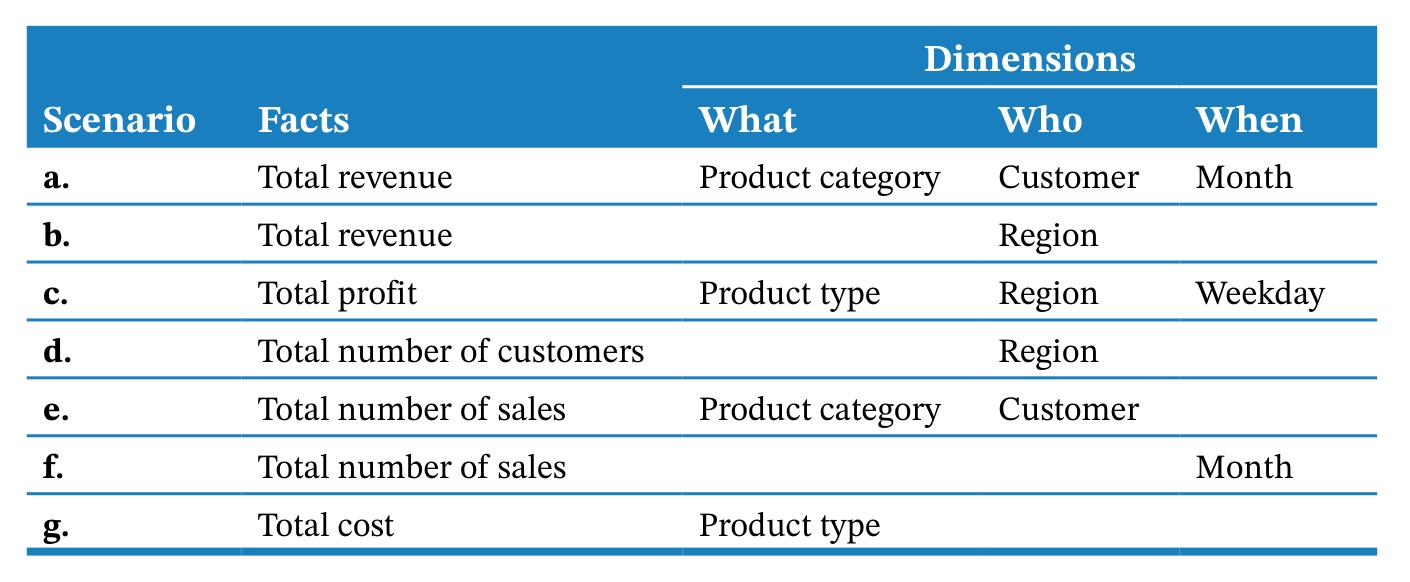
\includegraphics[width=0.95\textwidth,height=0.75\textheight,keepaspectratio]{../textbookForPractice/Figures/Ch_06/LO 1.5.png}
    \end{figure}
\end{frame}

\begin{frame}{LO 1.7}

    \begin{figure}[h]
        \centering
        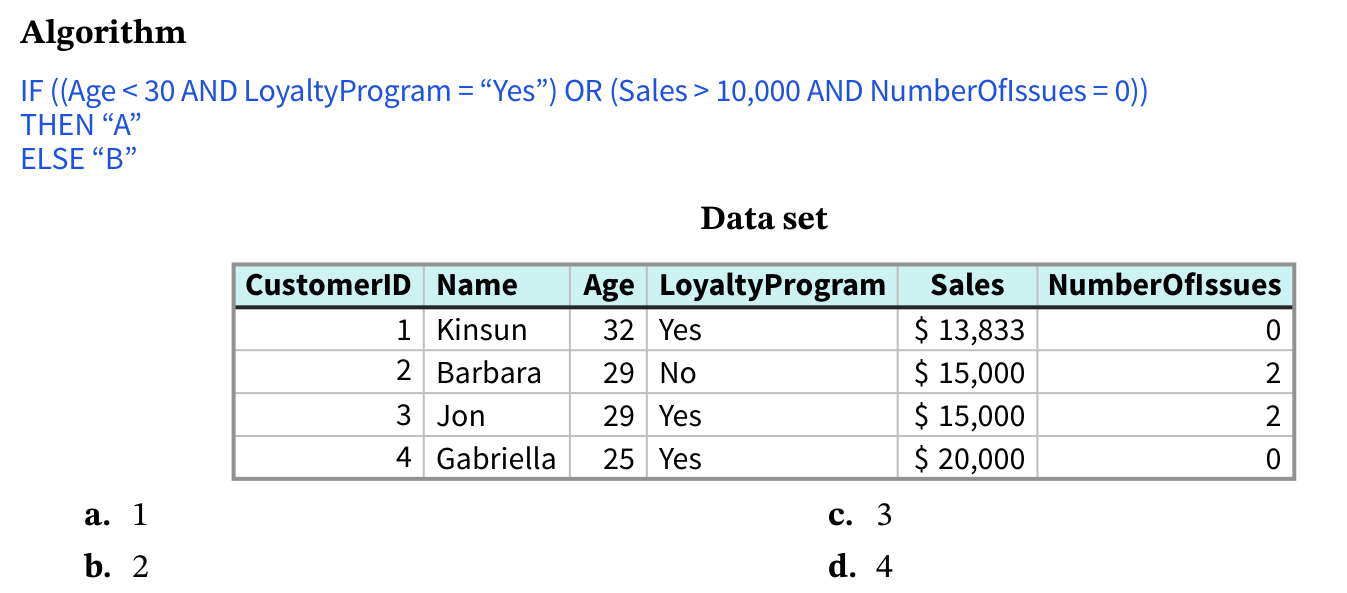
\includegraphics[width=0.95\textwidth,height=0.75\textheight,keepaspectratio]{../textbookForPractice/Figures/Ch_06/LO 1.7.png}
    \end{figure}
\end{frame}

\begin{frame}{LO 1.9}

    \begin{figure}[h]
        \centering
        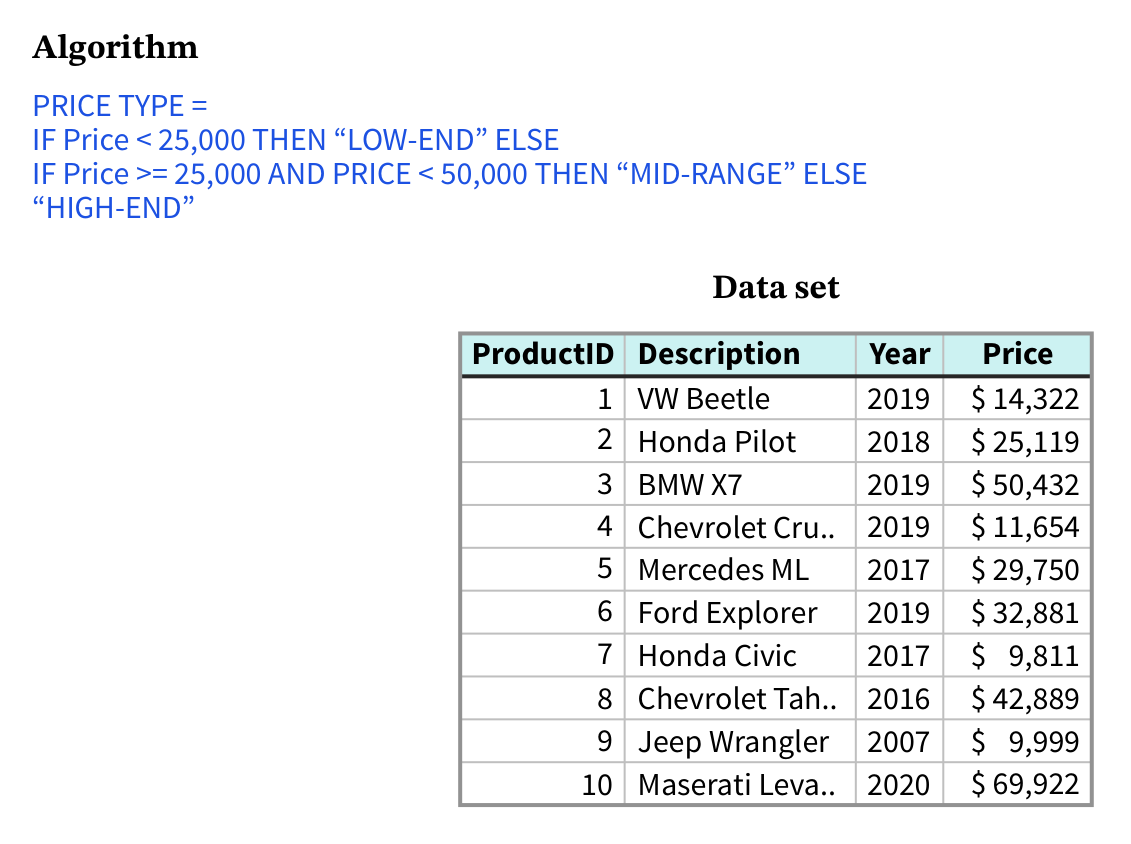
\includegraphics[width=0.95\textwidth,height=0.75\textheight,keepaspectratio]{../textbookForPractice/Figures/Ch_06/LO 1.9.png}
    \end{figure}
\end{frame}

\begin{frame}{LO 3.13}

    \begin{figure}[h]
        \centering
        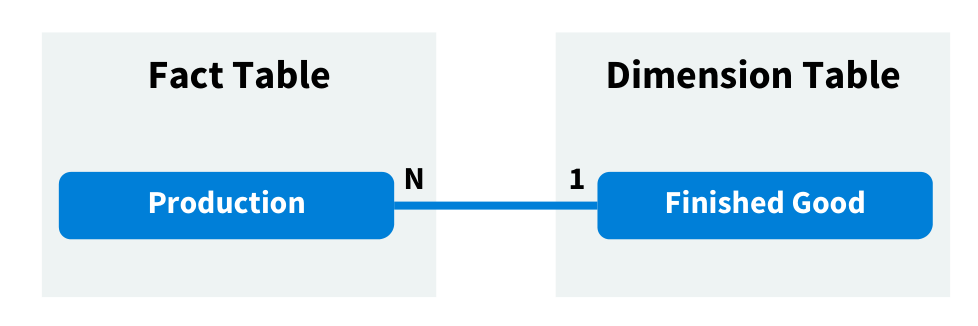
\includegraphics[width=0.95\textwidth,height=0.75\textheight,keepaspectratio]{../textbookForPractice/Figures/Ch_06/LO 3.13.png}
    \end{figure}
\end{frame}

\begin{frame}{LO 3.17}

    \begin{figure}[h]
        \centering
        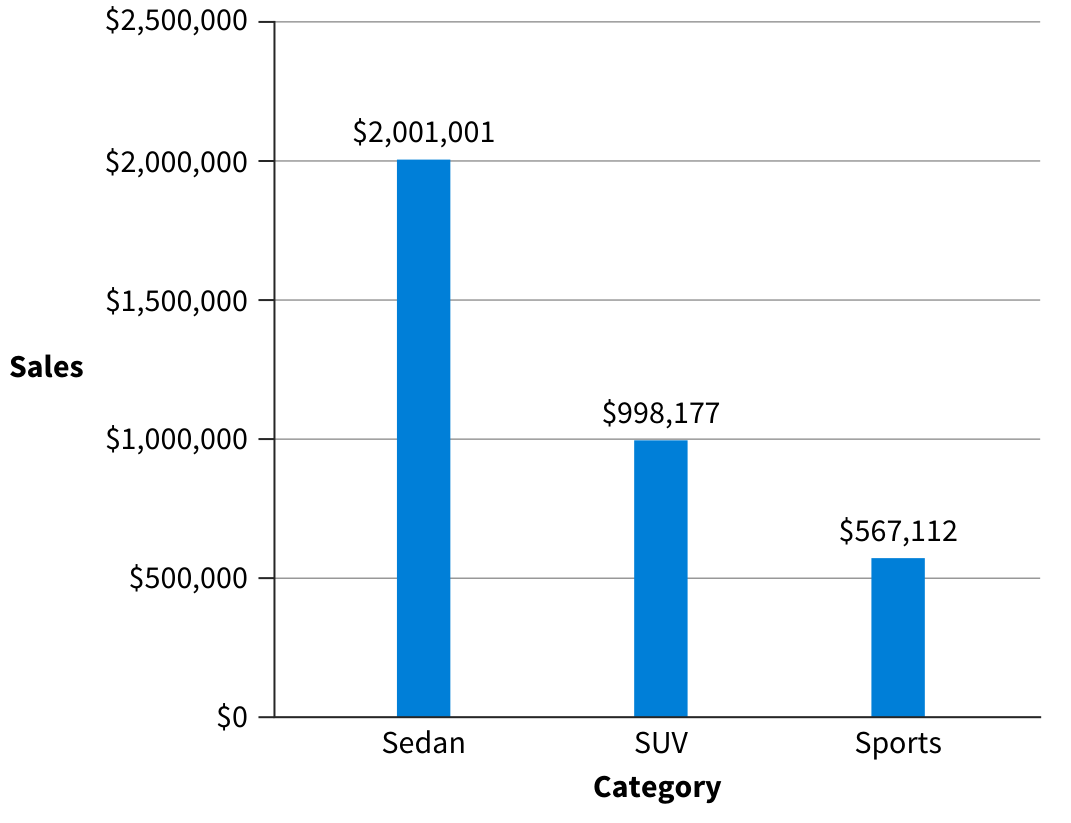
\includegraphics[width=0.95\textwidth,height=0.75\textheight,keepaspectratio]{../textbookForPractice/Figures/Ch_06/LO 3.17.png}
    \end{figure}
\end{frame}

\begin{frame}{LO 3.17\_1}

    \begin{figure}[h]
        \centering
        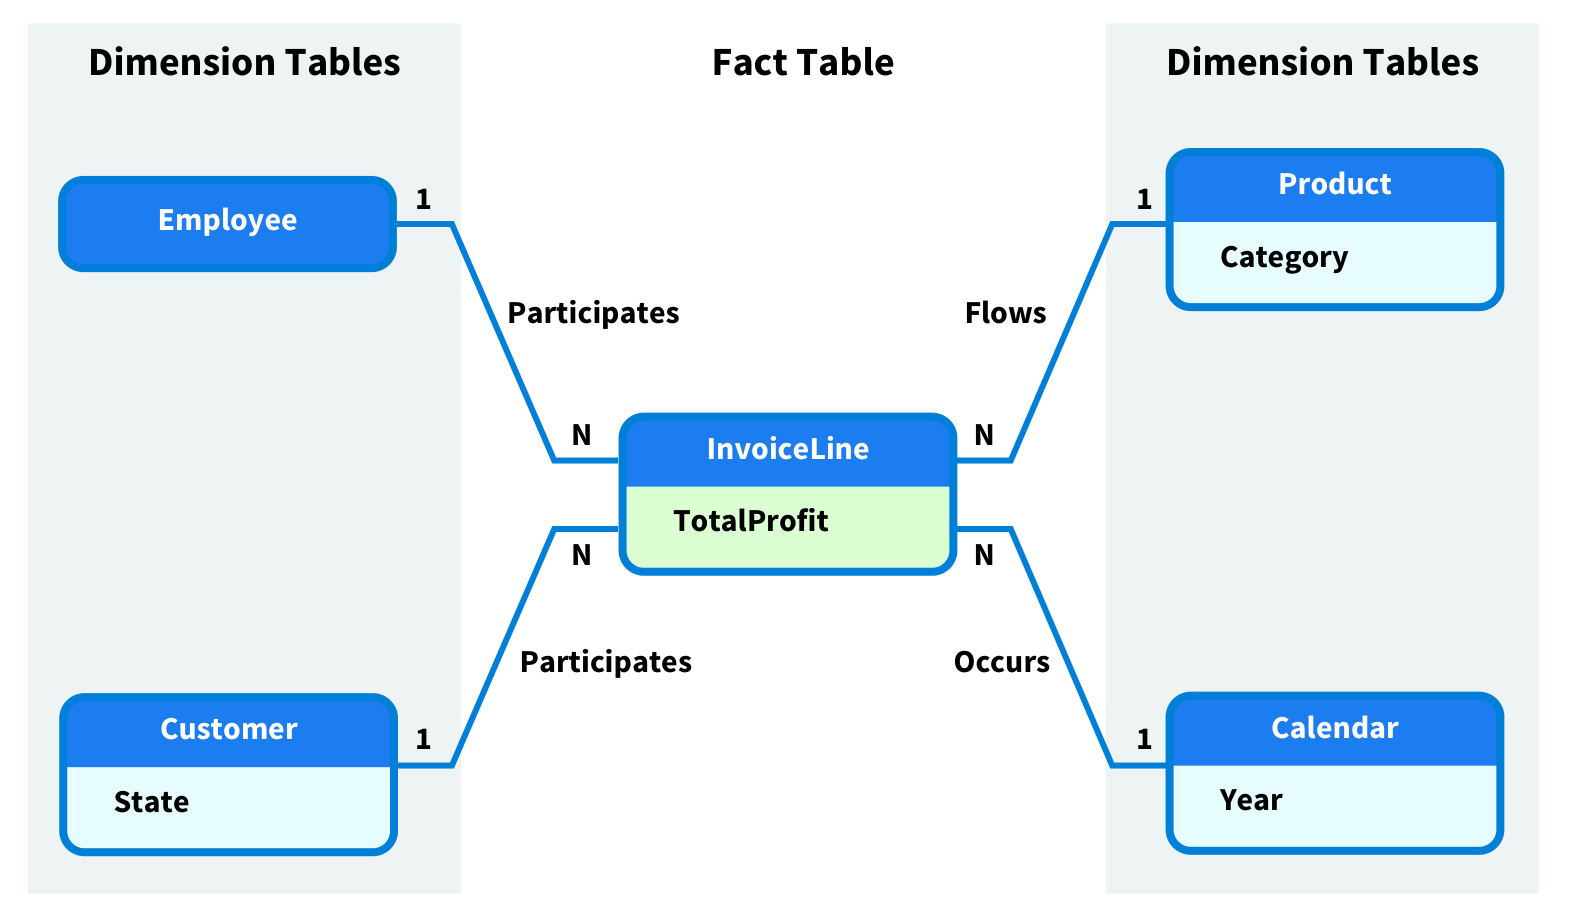
\includegraphics[width=0.95\textwidth,height=0.75\textheight,keepaspectratio]{../textbookForPractice/Figures/Ch_06/LO 3.17_1.png}
    \end{figure}
\end{frame}

\begin{frame}{LO 3.18}

    \begin{figure}[h]
        \centering
        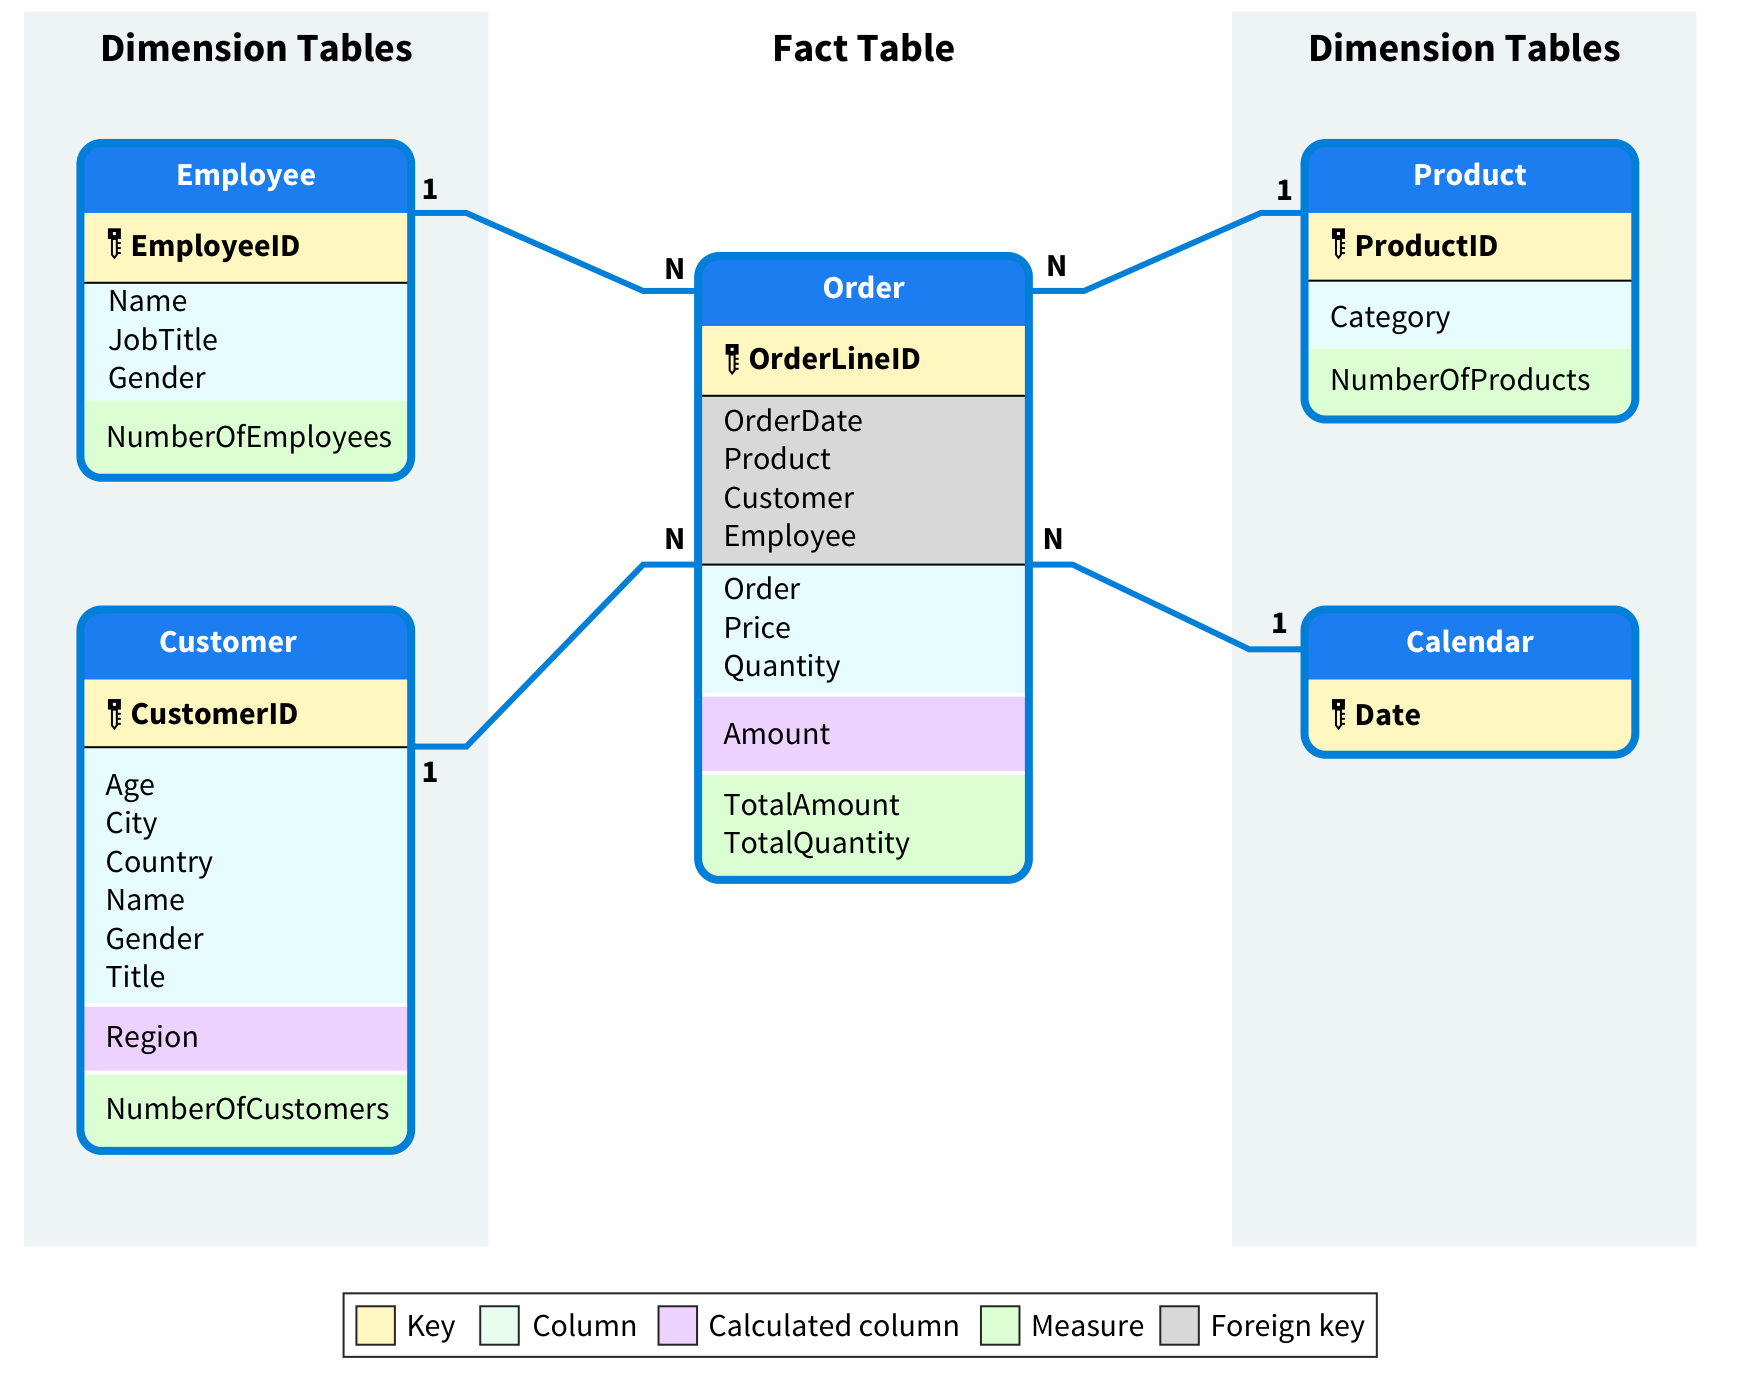
\includegraphics[width=0.95\textwidth,height=0.75\textheight,keepaspectratio]{../textbookForPractice/Figures/Ch_06/LO 3.18.png}
    \end{figure}
\end{frame}

\begin{frame}{LO 3.19}

    \begin{figure}[h]
        \centering
        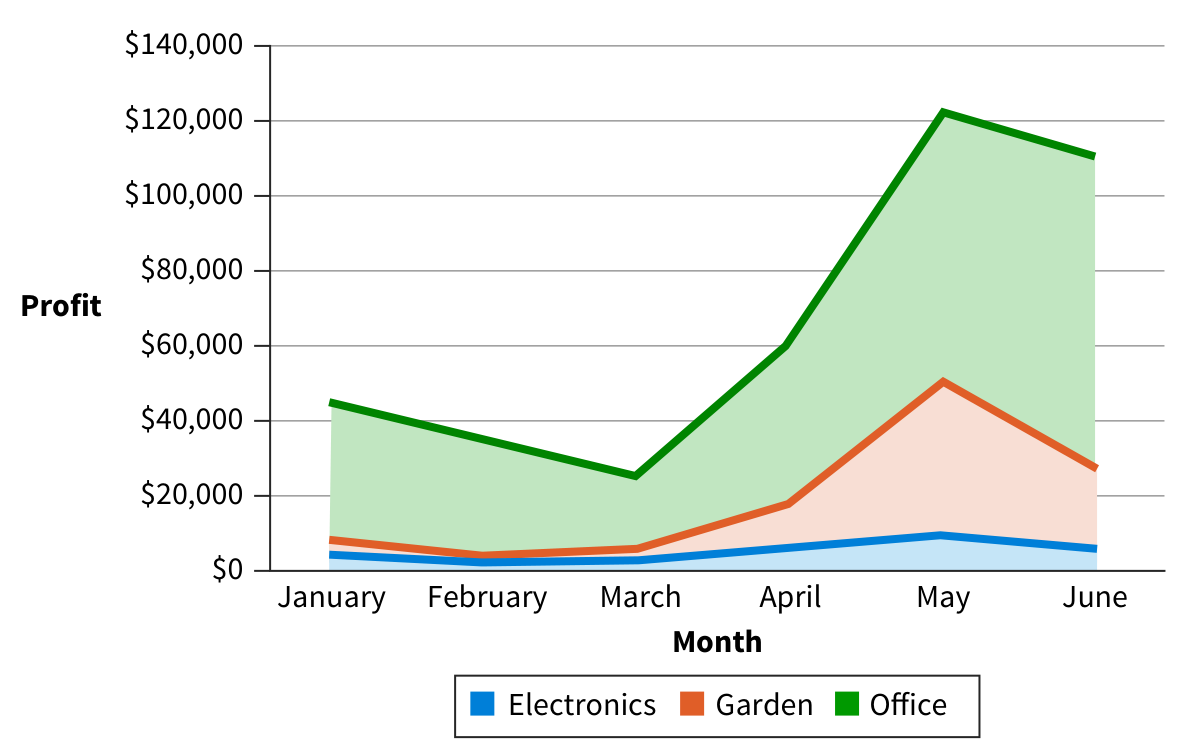
\includegraphics[width=0.95\textwidth,height=0.75\textheight,keepaspectratio]{../textbookForPractice/Figures/Ch_06/LO 3.19.png}
    \end{figure}
\end{frame}

\begin{frame}{LO 3.21}

    \begin{figure}[h]
        \centering
        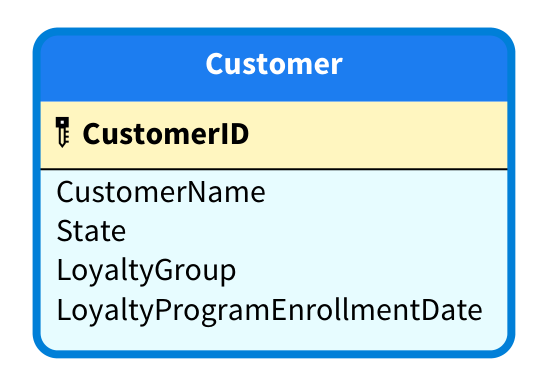
\includegraphics[width=0.95\textwidth,height=0.75\textheight,keepaspectratio]{../textbookForPractice/Figures/Ch_06/LO 3.21.png}
    \end{figure}
\end{frame}

\begin{frame}{DTunes data dictionary 6.0}

    \begin{figure}[h]
        \centering
        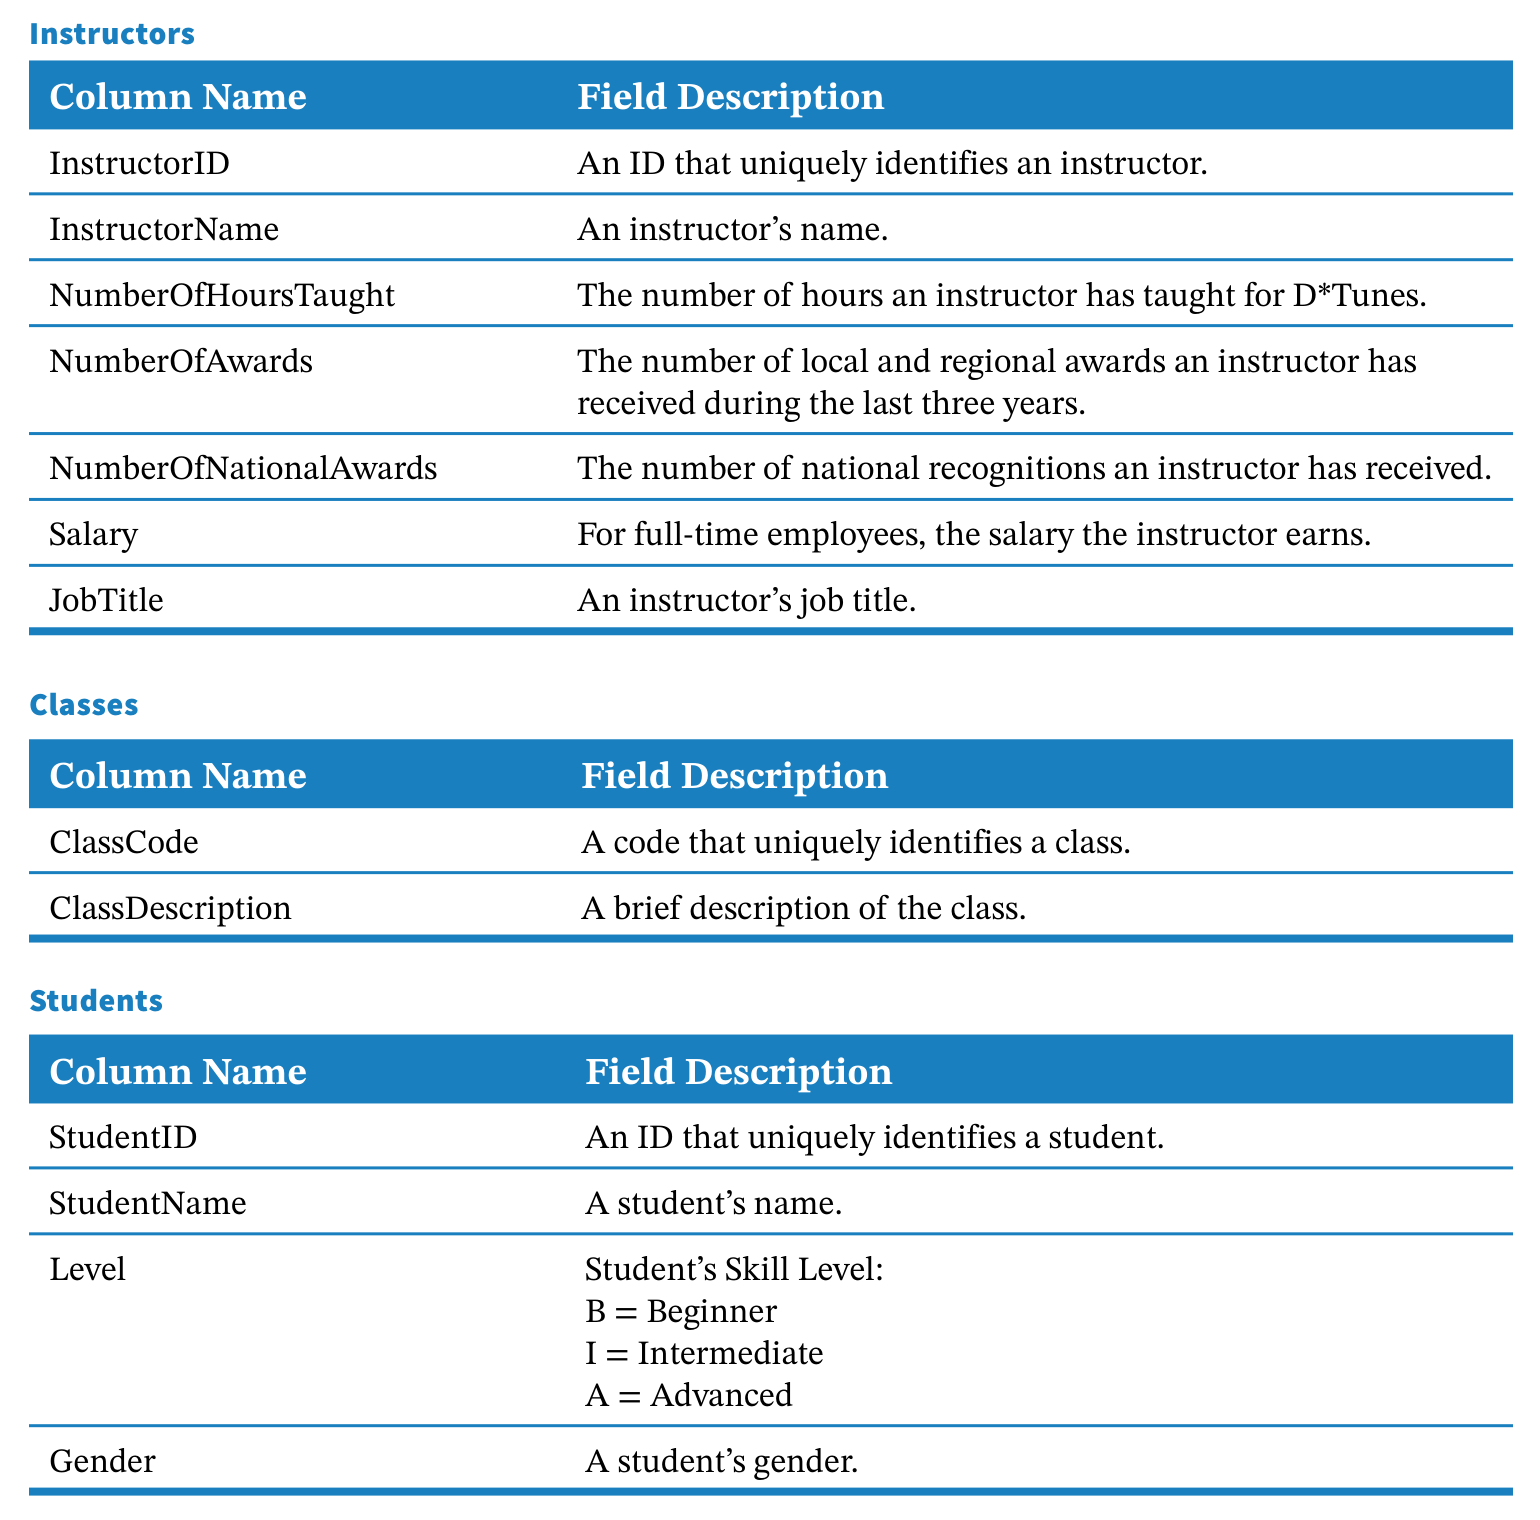
\includegraphics[width=0.95\textwidth,height=0.75\textheight,keepaspectratio]{../textbookForPractice/Figures/Ch_06/DTunes data dictionary 6.0.png}
    \end{figure}
\end{frame}

\begin{frame}{Fig 6.0}

    \begin{figure}[h]
        \centering
        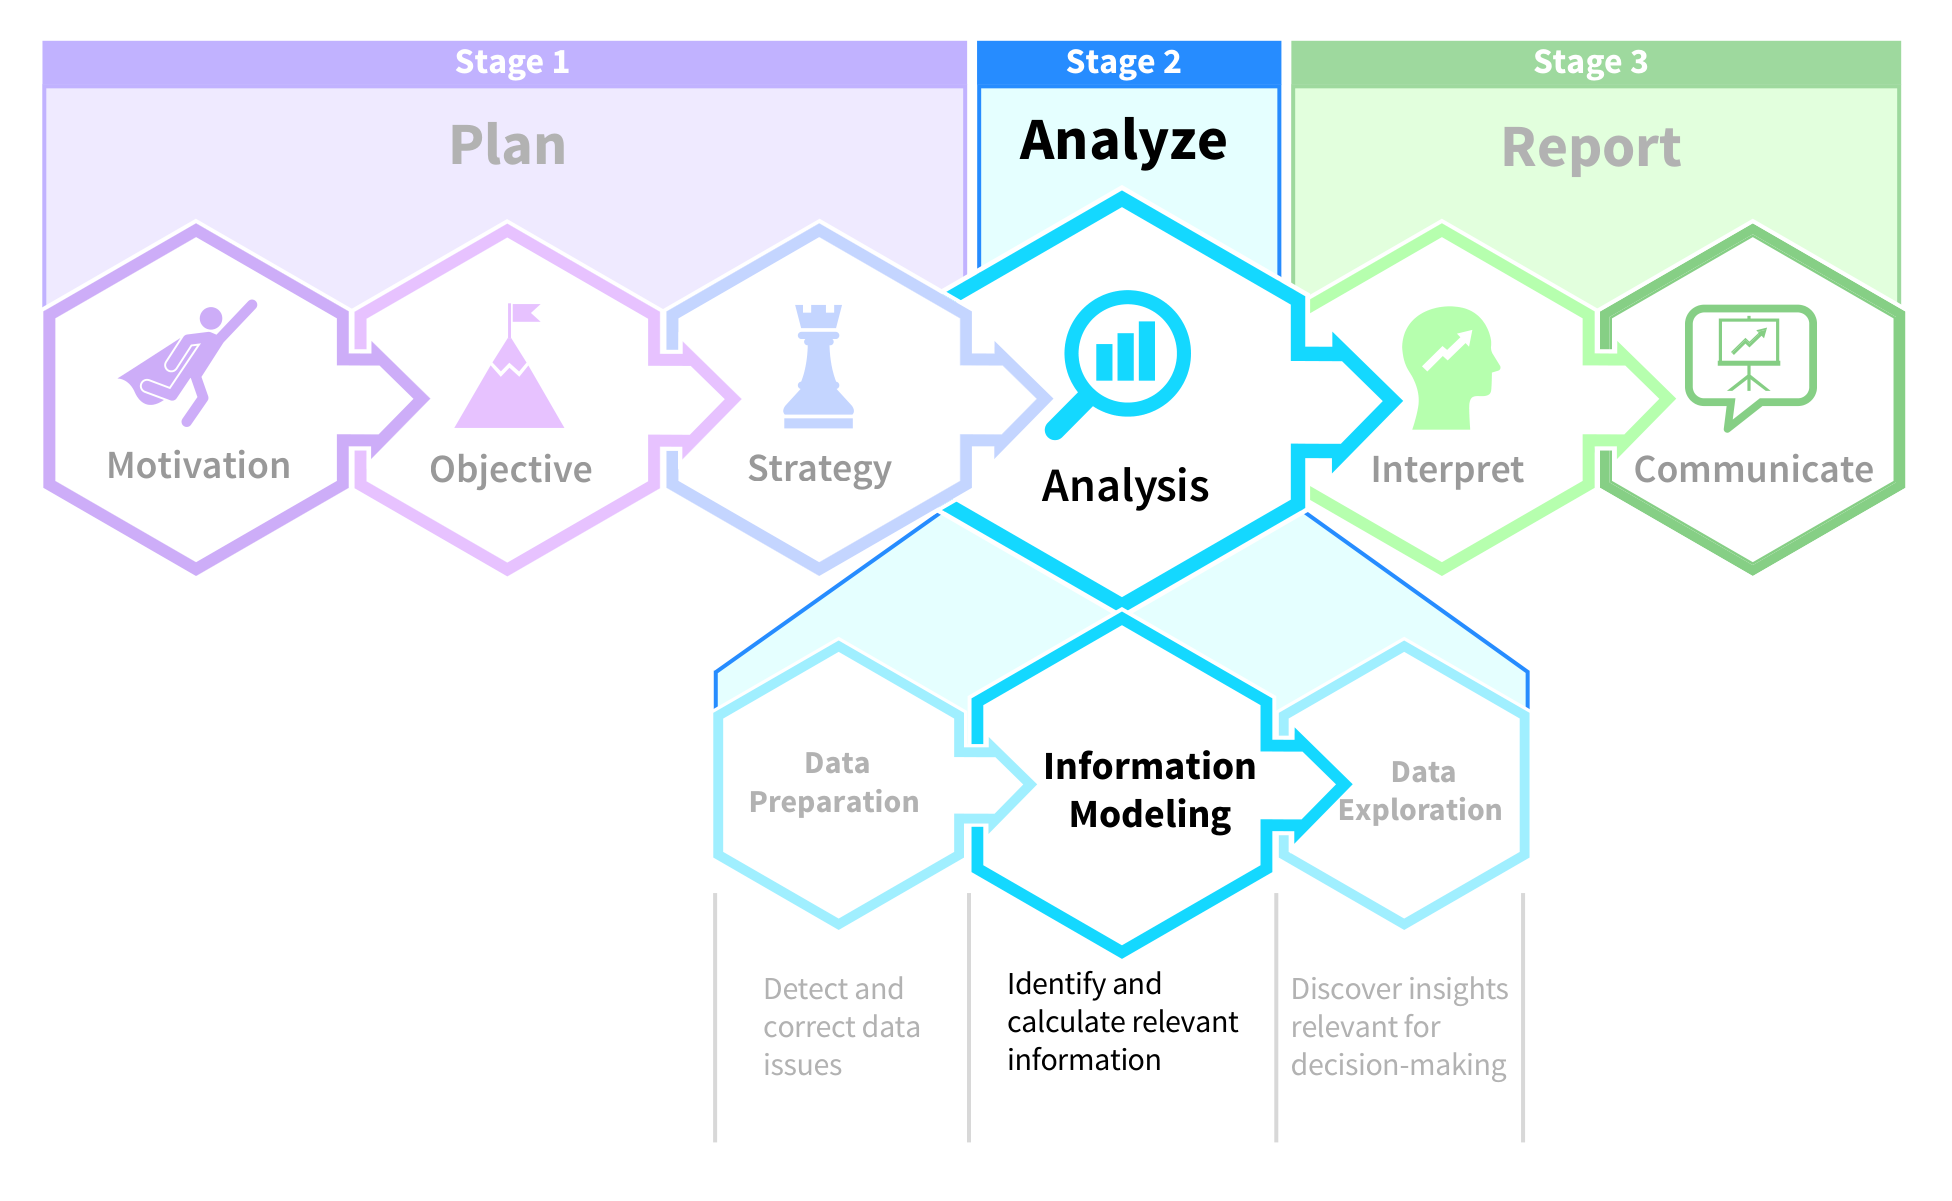
\includegraphics[width=0.95\textwidth,height=0.75\textheight,keepaspectratio]{../textbookForPractice/Figures/Ch_06/Fig 6.0.png}
    \end{figure}
\end{frame}

\begin{frame}{Apply It 6.1}

    \begin{figure}[h]
        \centering
        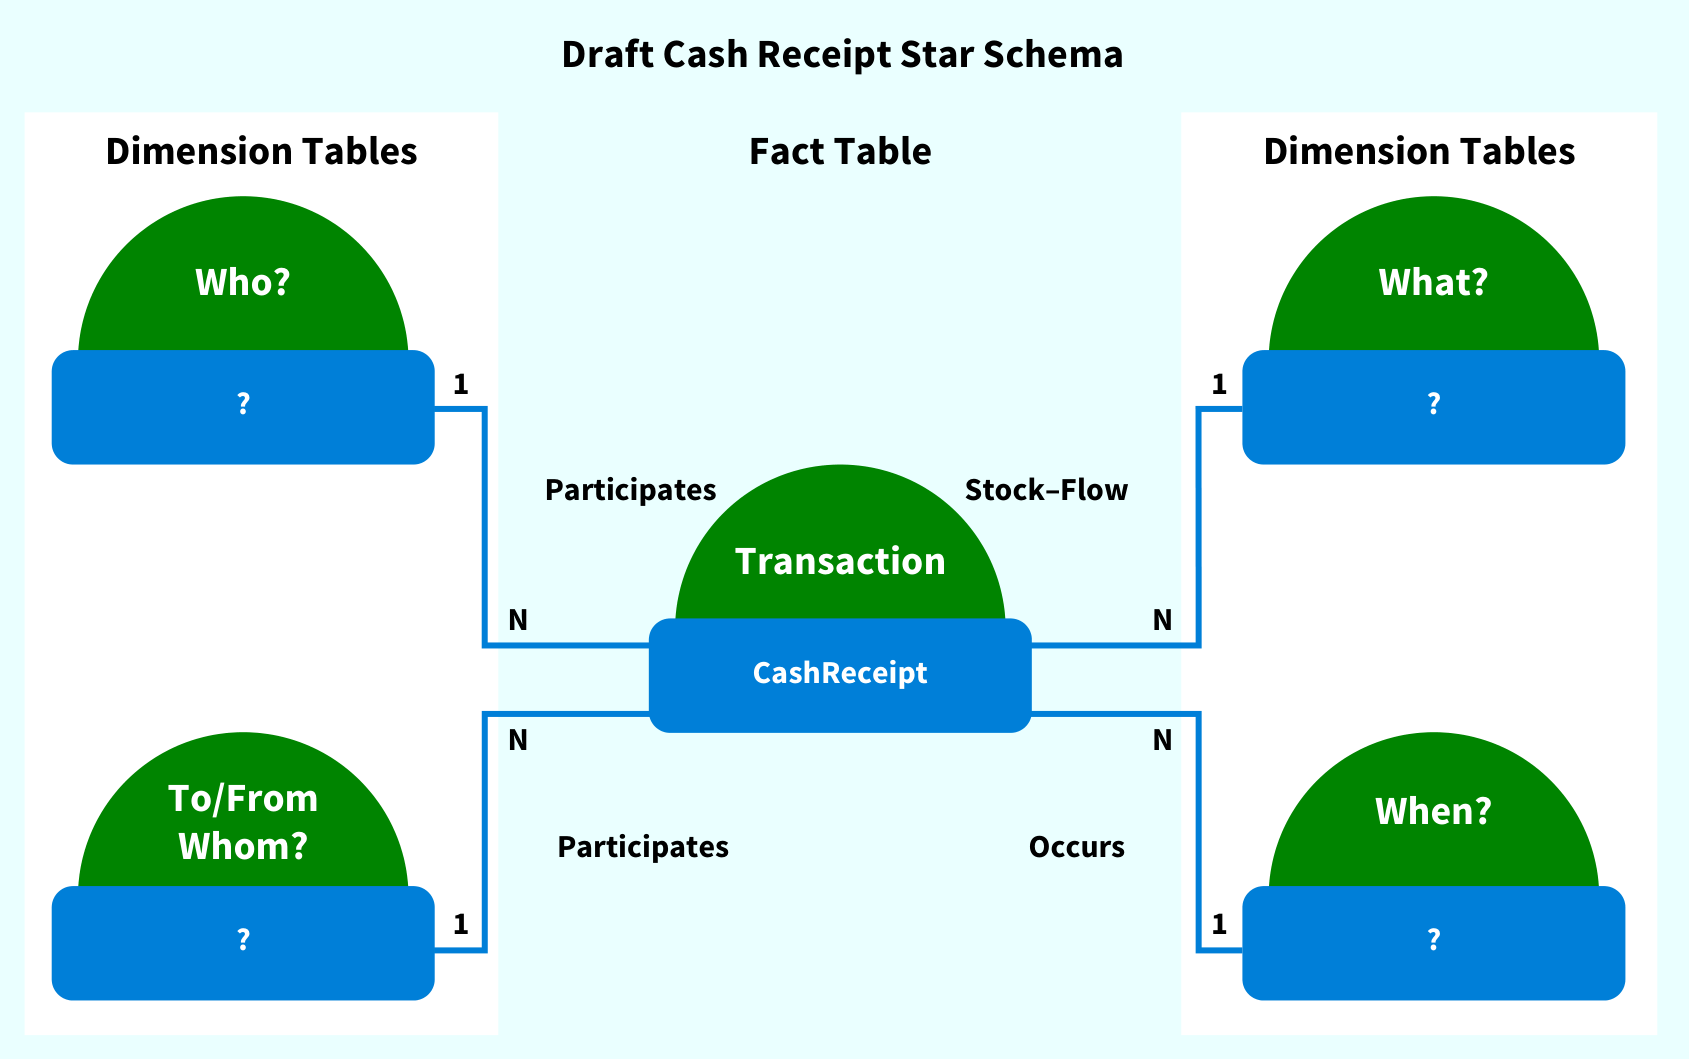
\includegraphics[width=0.95\textwidth,height=0.75\textheight,keepaspectratio]{../textbookForPractice/Figures/Ch_06/Apply It 6.1.png}
    \end{figure}
\end{frame}

\begin{frame}{DTunes data dictionary 6.1}

    \begin{figure}[h]
        \centering
        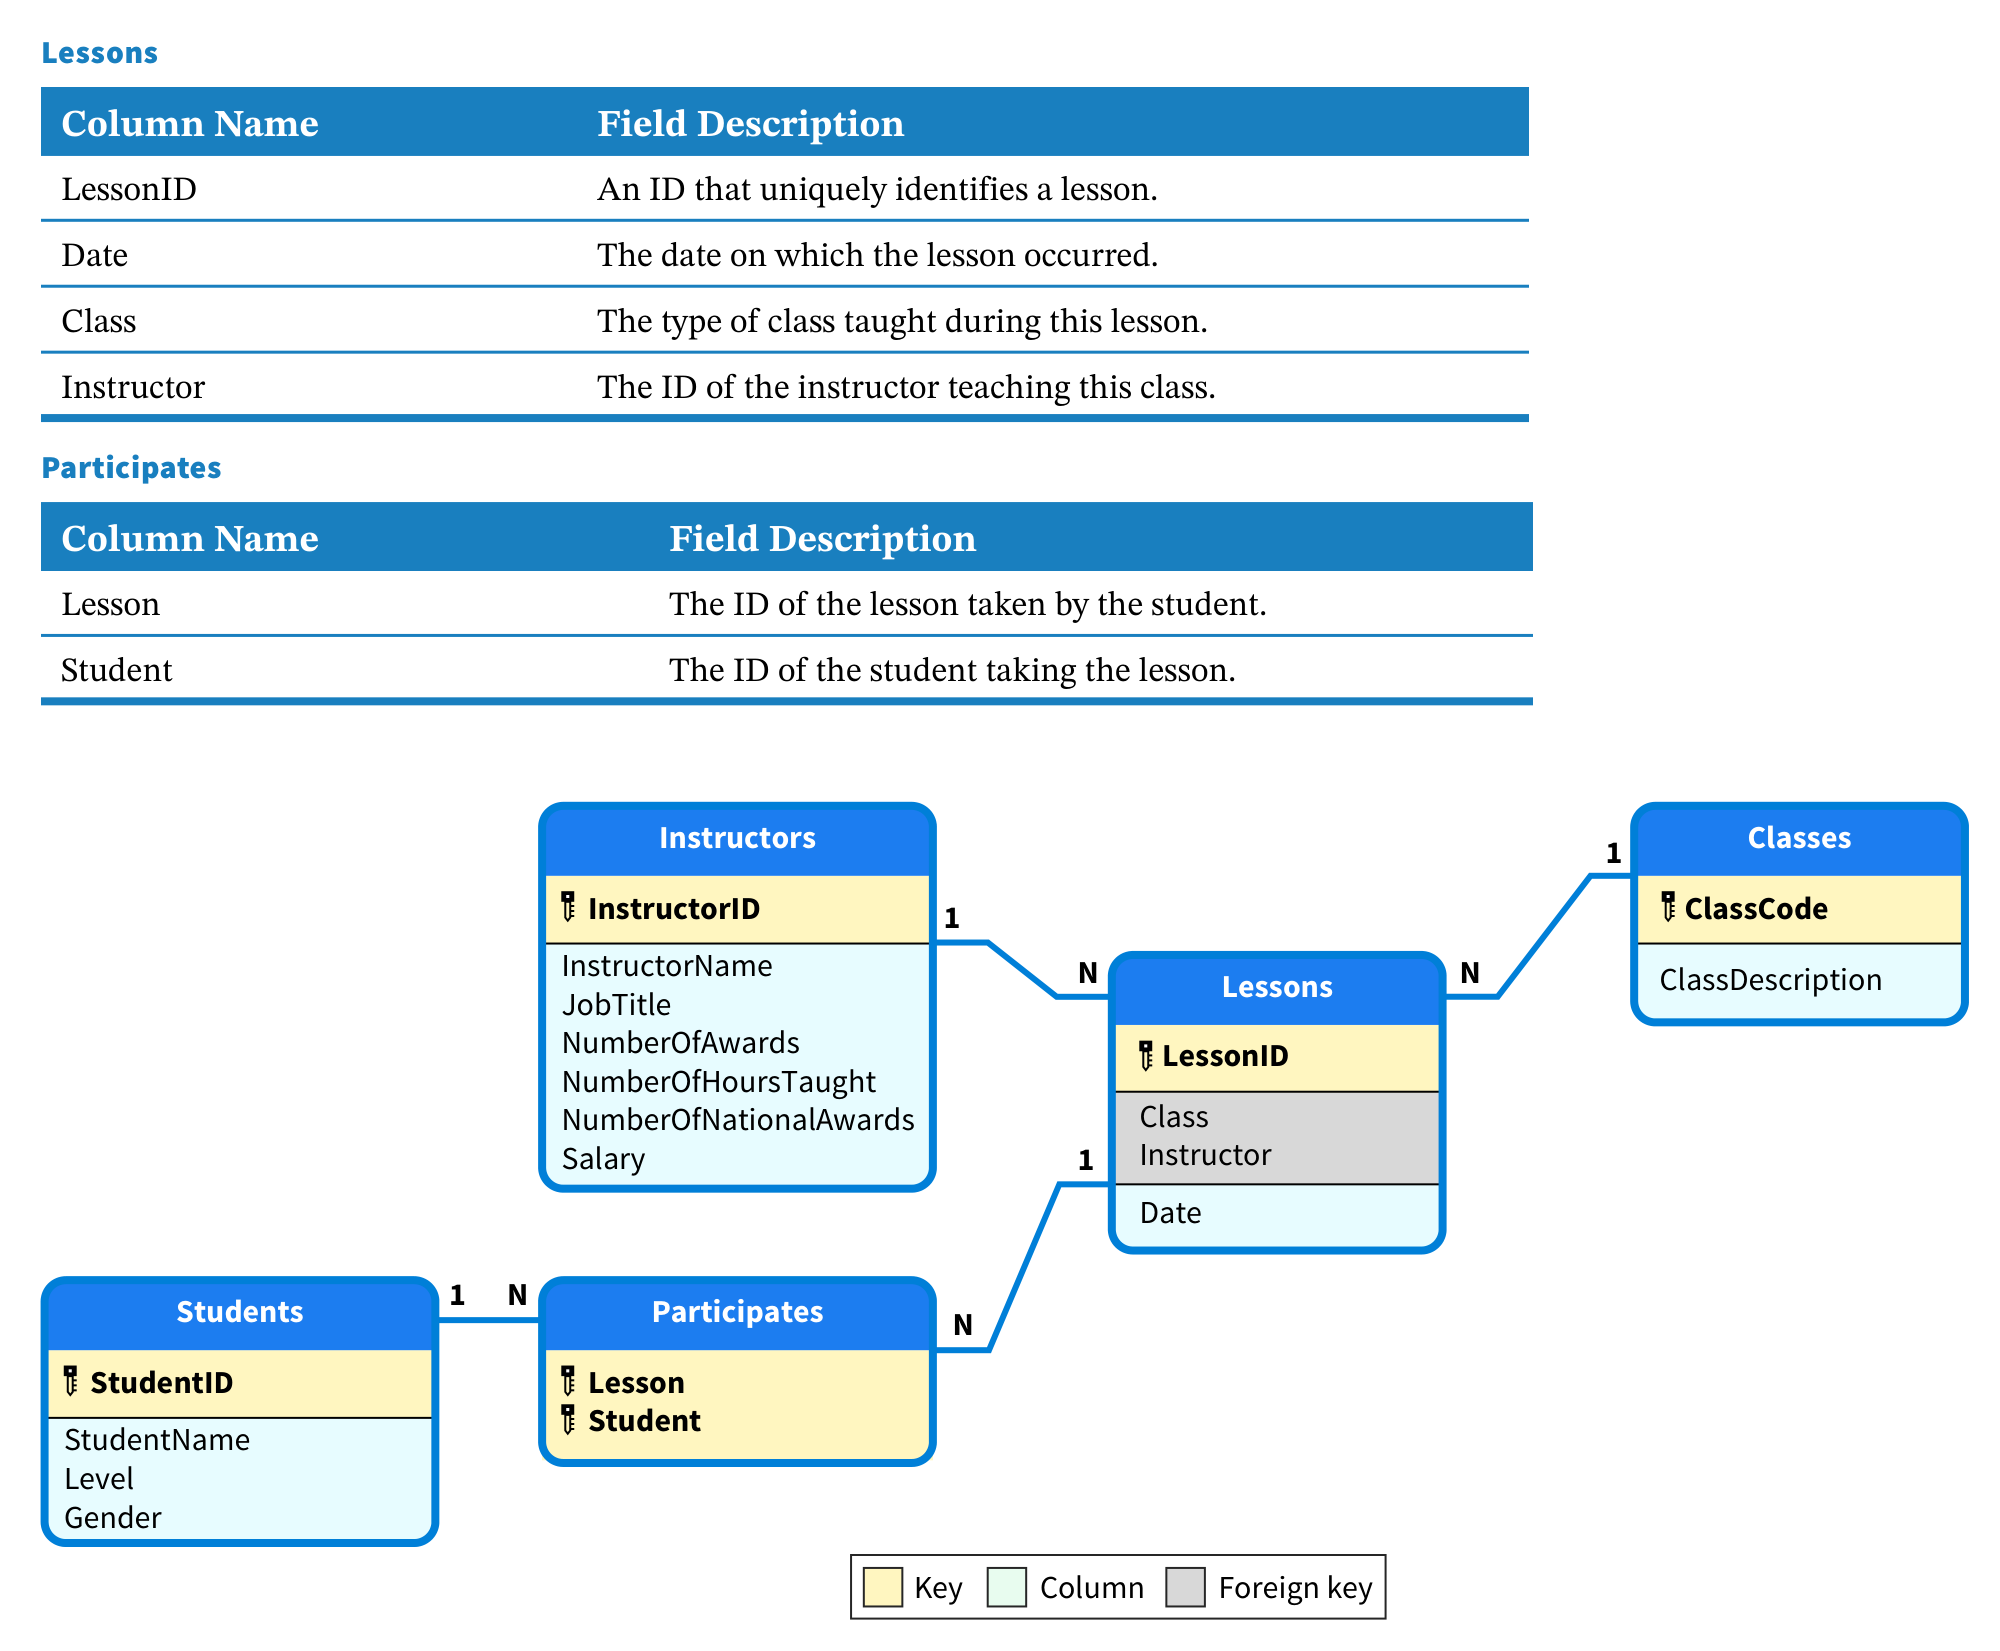
\includegraphics[width=0.95\textwidth,height=0.75\textheight,keepaspectratio]{../textbookForPractice/Figures/Ch_06/DTunes data dictionary 6.1.png}
    \end{figure}
\end{frame}

\begin{frame}{Apply It 6.2}

    \begin{figure}[h]
        \centering
        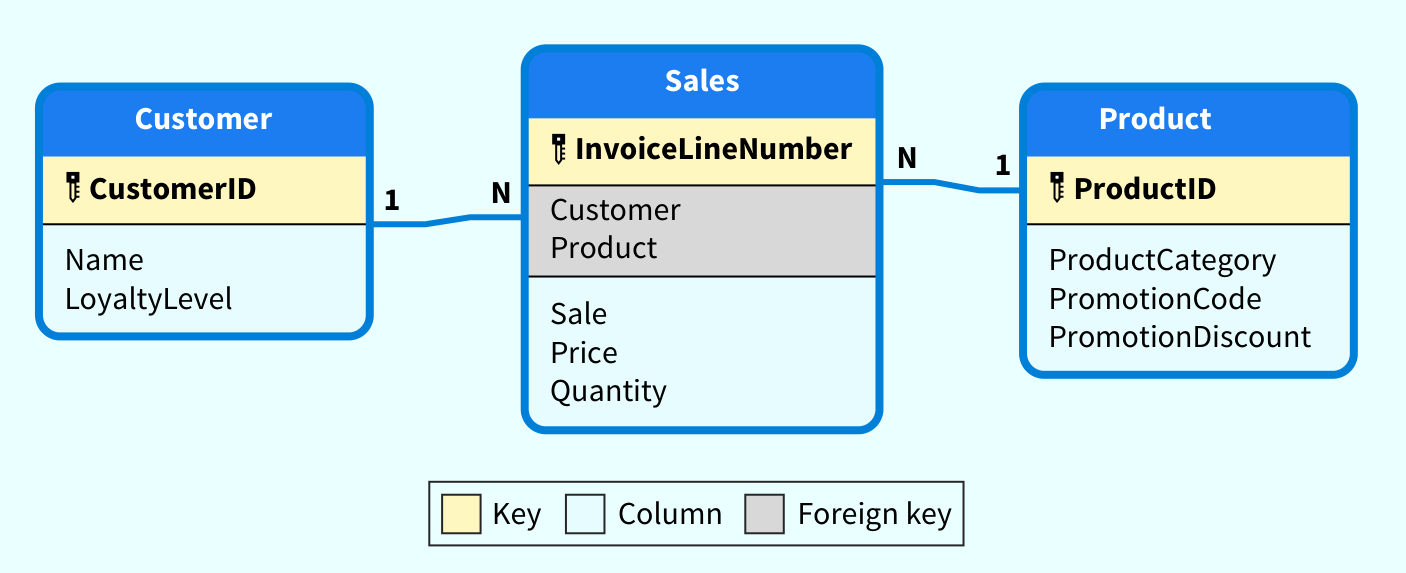
\includegraphics[width=0.95\textwidth,height=0.75\textheight,keepaspectratio]{../textbookForPractice/Figures/Ch_06/Apply It 6.2.png}
    \end{figure}
\end{frame}

\begin{frame}{Apply It 6.3}

    \begin{figure}[h]
        \centering
        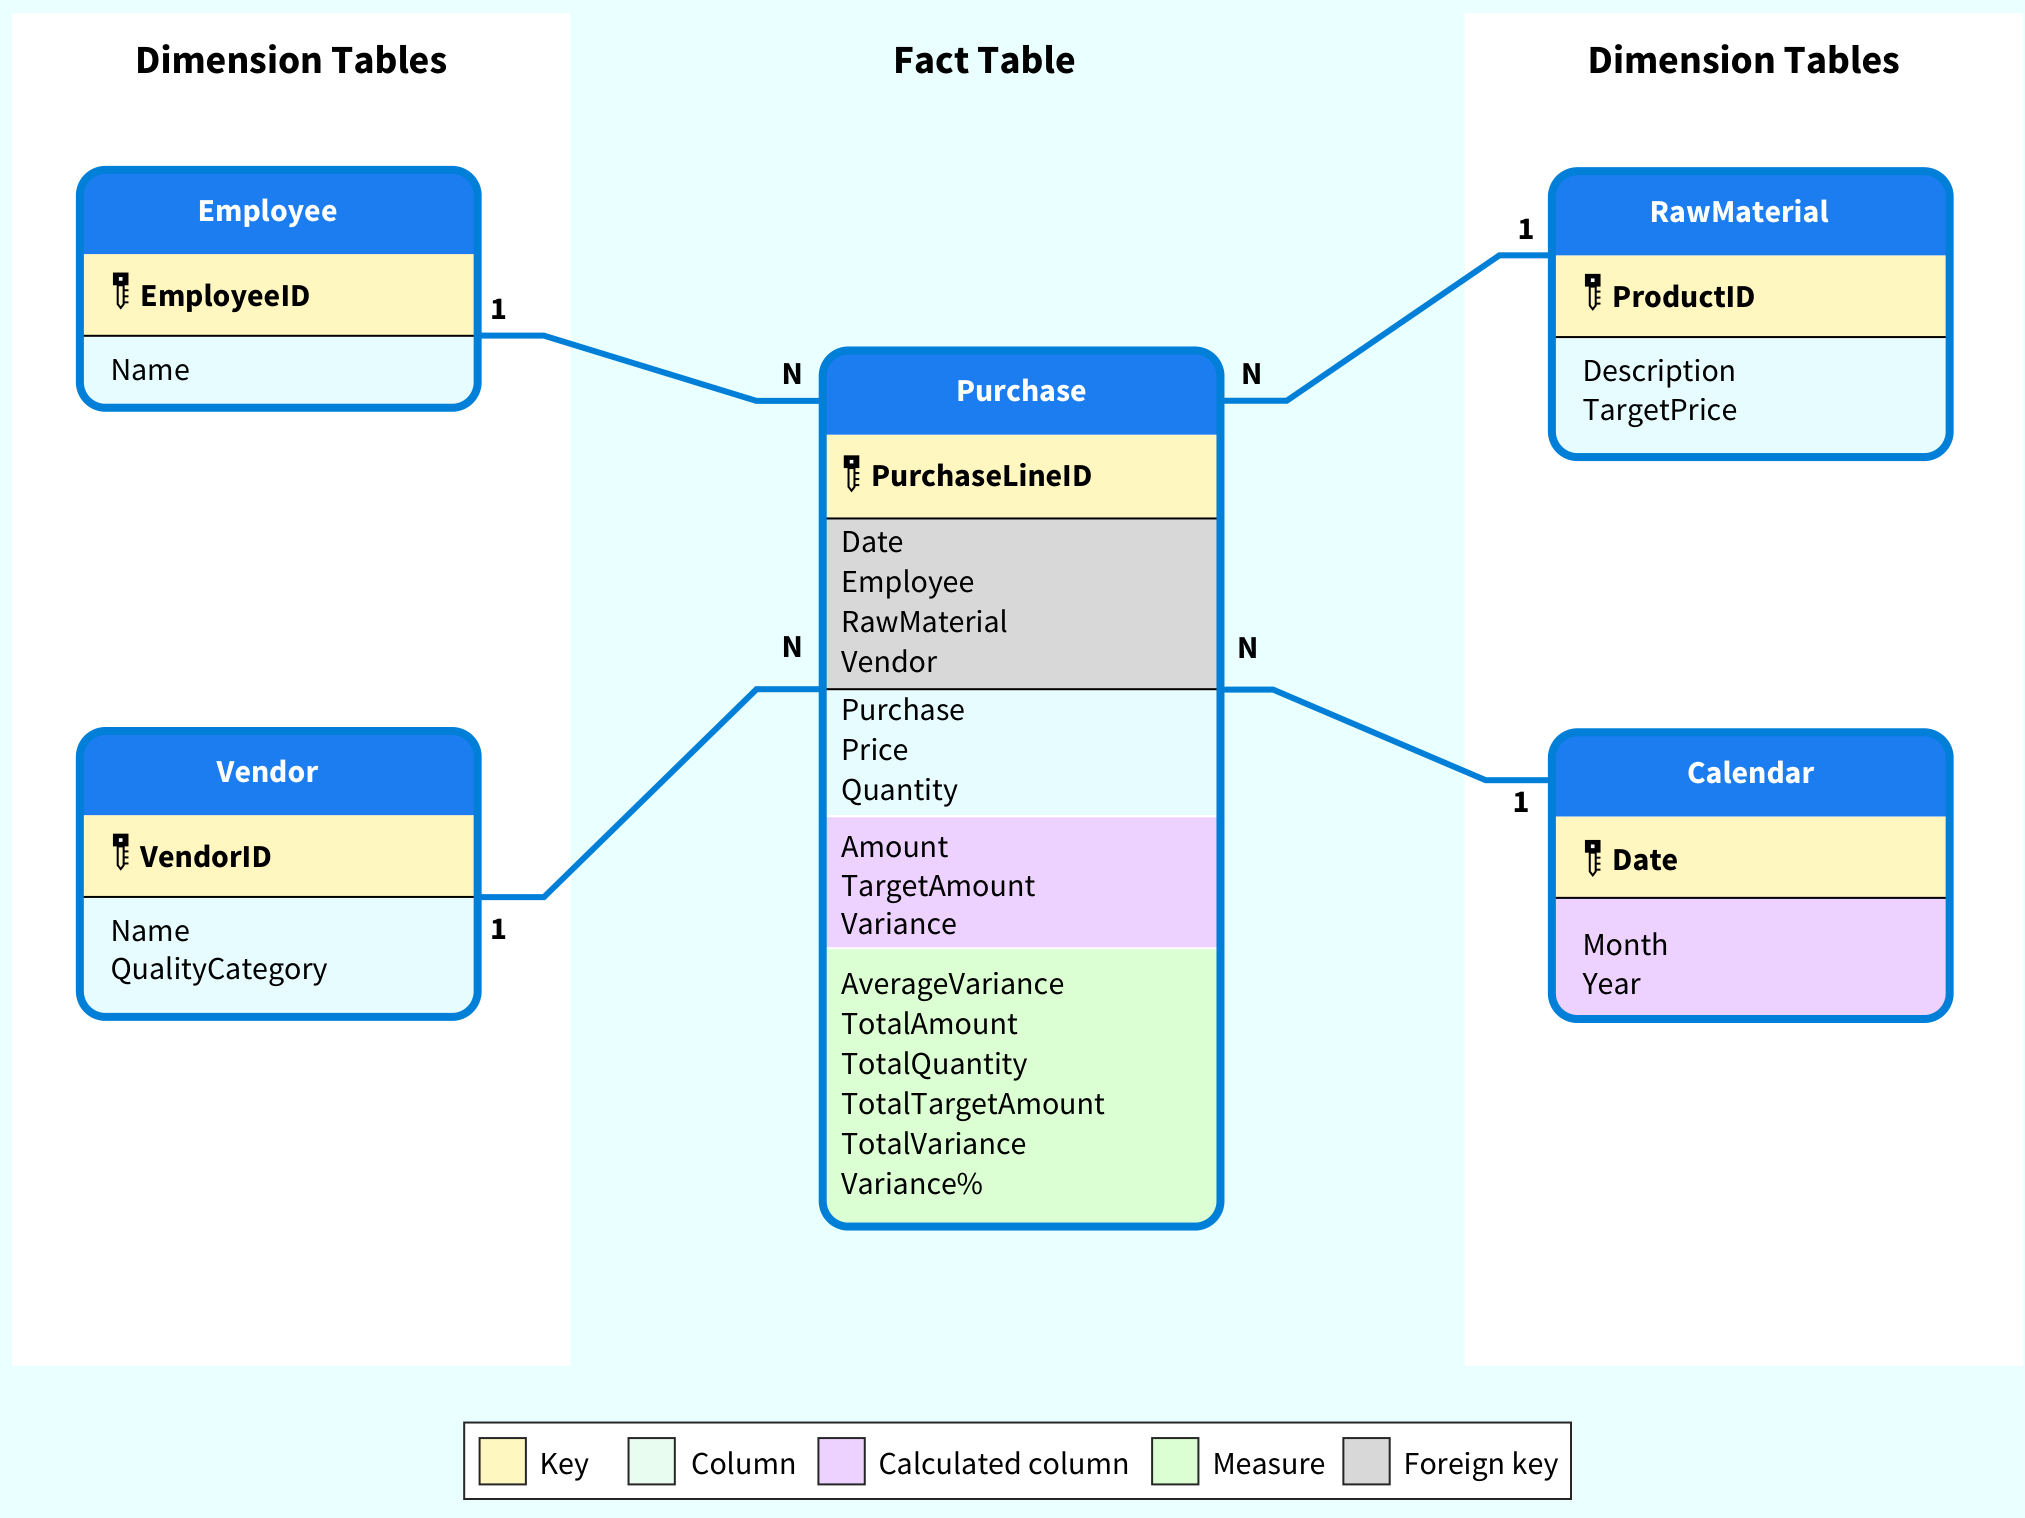
\includegraphics[width=0.95\textwidth,height=0.75\textheight,keepaspectratio]{../textbookForPractice/Figures/Ch_06/Apply It 6.3.png}
    \end{figure}
\end{frame}

\begin{frame}{Kết thúc}
    \begin{center}
        \Huge \textbf{Hỏi \& Đáp} \\
        \vspace{1cm}
        \Large Cảm ơn các bạn đã lắng nghe!
    \end{center}
\end{frame}

\end{document}
